\documentclass[twoside]{book}

% Packages required by doxygen
\usepackage{fixltx2e}
\usepackage{calc}
\usepackage{doxygen}
\usepackage[export]{adjustbox} % also loads graphicx
\usepackage{graphicx}
\usepackage[utf8]{inputenc}
\usepackage{makeidx}
\usepackage{multicol}
\usepackage{multirow}
\PassOptionsToPackage{warn}{textcomp}
\usepackage{textcomp}
\usepackage[nointegrals]{wasysym}
\usepackage[table]{xcolor}

% NLS support packages
\usepackage[french]{babel}

% Font selection
\usepackage[T1]{fontenc}
\usepackage[scaled=.90]{helvet}
\usepackage{courier}
\usepackage{amssymb}
\usepackage{sectsty}
\renewcommand{\familydefault}{\sfdefault}
\allsectionsfont{%
  \fontseries{bc}\selectfont%
  \color{darkgray}%
}
\renewcommand{\DoxyLabelFont}{%
  \fontseries{bc}\selectfont%
  \color{darkgray}%
}
\newcommand{\+}{\discretionary{\mbox{\scriptsize$\hookleftarrow$}}{}{}}

% Page & text layout
\usepackage{geometry}
\geometry{%
  a4paper,%
  top=2.5cm,%
  bottom=2.5cm,%
  left=2.5cm,%
  right=2.5cm%
}
\tolerance=750
\hfuzz=15pt
\hbadness=750
\setlength{\emergencystretch}{15pt}
\setlength{\parindent}{0cm}
\setlength{\parskip}{3ex plus 2ex minus 2ex}
\makeatletter
\renewcommand{\paragraph}{%
  \@startsection{paragraph}{4}{0ex}{-1.0ex}{1.0ex}{%
    \normalfont\normalsize\bfseries\SS@parafont%
  }%
}
\renewcommand{\subparagraph}{%
  \@startsection{subparagraph}{5}{0ex}{-1.0ex}{1.0ex}{%
    \normalfont\normalsize\bfseries\SS@subparafont%
  }%
}
\makeatother

% Headers & footers
\usepackage{fancyhdr}
\pagestyle{fancyplain}
\fancyhead[LE]{\fancyplain{}{\bfseries\thepage}}
\fancyhead[CE]{\fancyplain{}{}}
\fancyhead[RE]{\fancyplain{}{\bfseries\leftmark}}
\fancyhead[LO]{\fancyplain{}{\bfseries\rightmark}}
\fancyhead[CO]{\fancyplain{}{}}
\fancyhead[RO]{\fancyplain{}{\bfseries\thepage}}
\fancyfoot[LE]{\fancyplain{}{}}
\fancyfoot[CE]{\fancyplain{}{}}
\fancyfoot[RE]{\fancyplain{}{\bfseries\scriptsize Généré par Doxygen }}
\fancyfoot[LO]{\fancyplain{}{\bfseries\scriptsize Généré par Doxygen }}
\fancyfoot[CO]{\fancyplain{}{}}
\fancyfoot[RO]{\fancyplain{}{}}
\renewcommand{\footrulewidth}{0.4pt}
\renewcommand{\chaptermark}[1]{%
  \markboth{#1}{}%
}
\renewcommand{\sectionmark}[1]{%
  \markright{\thesection\ #1}%
}

% Indices & bibliography
\usepackage{natbib}
\usepackage[titles]{tocloft}
\setcounter{tocdepth}{3}
\setcounter{secnumdepth}{5}
\makeindex

% Hyperlinks (required, but should be loaded last)
\usepackage{ifpdf}
\ifpdf
  \usepackage[pdftex,pagebackref=true]{hyperref}
\else
  \usepackage[ps2pdf,pagebackref=true]{hyperref}
\fi
\hypersetup{%
  colorlinks=true,%
  linkcolor=blue,%
  citecolor=blue,%
  unicode%
}

% Custom commands
\newcommand{\clearemptydoublepage}{%
  \newpage{\pagestyle{empty}\cleardoublepage}%
}

\usepackage{caption}
\captionsetup{labelsep=space,justification=centering,font={bf},singlelinecheck=off,skip=4pt,position=top}

%===== C O N T E N T S =====

\begin{document}

% Titlepage & ToC
\hypersetup{pageanchor=false,
             bookmarksnumbered=true,
             pdfencoding=unicode
            }
\pagenumbering{roman}
\begin{titlepage}
\vspace*{7cm}
\begin{center}%
{\Large My Project }\\
\vspace*{1cm}
{\large Généré par Doxygen 1.8.11}\\
\end{center}
\end{titlepage}
\clearemptydoublepage
\tableofcontents
\clearemptydoublepage
\pagenumbering{arabic}
\hypersetup{pageanchor=true}

%--- Begin generated contents ---
\chapter{T\+HE Monopoly}
\label{index}\hypertarget{index}{}\hypertarget{index_intro_sec}{}\section{Introduction}\label{index_intro_sec}
Le projet T\+HE Monopoly concu dans le cadre de l\textquotesingle{}UE L\+I\+F\+A\+P4. ~\newline
 Code ecrit en C/\+C++.\hypertarget{index_compile_sec}{}\section{Pour compiler, ouvrir un terminal}\label{index_compile_sec}
a la racine et ecrire \char`\"{}make\char`\"{}.\hypertarget{index_exec_sec}{}\section{Pour executer, apres la compilation,}\label{index_exec_sec}
ouvrir un terminal dans le dossier \char`\"{}bin\char`\"{} et ecrire \+: \char`\"{}./monopoly\+\_\+txt\char`\"{} pour le mode texte ~\newline
 \char`\"{}./monopoly\+\_\+sdl\char`\"{} pour la version graphique.

Generer la documentation du code. Taper \char`\"{}doxygen -\/g doc/image.\+doxy\char`\"{} puis \char`\"{}doxygen doc/image.\+doxy\char`\"{} dans un terminal ouvert a la racine. ~\newline
 Ensuite ecrire \char`\"{}firefox html/index.\+html\char`\"{} dans le dossier \char`\"{}doc\char`\"{} ou alors \char`\"{}firefox doc/html/index.\+html\char`\"{} à la racine. 
\chapter{Index des classes}
\section{Liste des classes}
Liste des classes, structures, unions et interfaces avec une brève description \+:\begin{DoxyCompactList}
\item\contentsline{section}{\hyperlink{classCarte}{Carte} }{\pageref{classCarte}}{}
\item\contentsline{section}{\hyperlink{classCase}{Case} }{\pageref{classCase}}{}
\item\contentsline{section}{\hyperlink{structPaquetCaisseComm_1_1Cellule}{Paquet\+Caisse\+Comm\+::\+Cellule} }{\pageref{structPaquetCaisseComm_1_1Cellule}}{}
\item\contentsline{section}{\hyperlink{structPaquetChance_1_1Cellule}{Paquet\+Chance\+::\+Cellule} }{\pageref{structPaquetChance_1_1Cellule}}{}
\item\contentsline{section}{\hyperlink{classCouleur}{Couleur} }{\pageref{classCouleur}}{}
\item\contentsline{section}{\hyperlink{classDe}{De} }{\pageref{classDe}}{}
\item\contentsline{section}{\hyperlink{classImage}{Image} \\*Pour g�rer une image avec S\+D\+L2 }{\pageref{classImage}}{}
\item\contentsline{section}{\hyperlink{classJeu}{Jeu} }{\pageref{classJeu}}{}
\item\contentsline{section}{\hyperlink{classJoueur}{Joueur} }{\pageref{classJoueur}}{}
\item\contentsline{section}{\hyperlink{classPaquetCaisseComm}{Paquet\+Caisse\+Comm} }{\pageref{classPaquetCaisseComm}}{}
\item\contentsline{section}{\hyperlink{classPaquetChance}{Paquet\+Chance} }{\pageref{classPaquetChance}}{}
\item\contentsline{section}{\hyperlink{classPlateau}{Plateau} }{\pageref{classPlateau}}{}
\item\contentsline{section}{\hyperlink{classPropriete}{Propriete} }{\pageref{classPropriete}}{}
\item\contentsline{section}{\hyperlink{classsdlJeu}{sdl\+Jeu} }{\pageref{classsdlJeu}}{}
\end{DoxyCompactList}

\chapter{Index des fichiers}
\section{Liste des fichiers}
Liste de tous les fichiers documentés avec une brève description \+:\begin{DoxyCompactList}
\item\contentsline{section}{src/sdl2/\hyperlink{main__sdl_8cpp}{main\+\_\+sdl.\+cpp} \\*Ce fichier contient le programme principal de T\+HE monopoly en S\+D\+L2 }{\pageref{main__sdl_8cpp}}{}
\item\contentsline{section}{src/sdl2/\hyperlink{sdlJeu_8cpp}{sdl\+Jeu.\+cpp} \\*Ce fichier contient les fonctions relatives a la gestion de l\textquotesingle{}affichage sdl ainsi qu\textquotesingle{}a la gestion des images }{\pageref{sdlJeu_8cpp}}{}
\item\contentsline{section}{src/sdl2/\hyperlink{sdlJeu_8h}{sdl\+Jeu.\+h} \\*Ce fichier contient les en-\/tetes des fonctions relatives a la gestion de l\textquotesingle{}affichage sdl ainsi qu\textquotesingle{}a la gestion des images }{\pageref{sdlJeu_8h}}{}
\item\contentsline{section}{src/txt/\hyperlink{Carte_8cpp}{Carte.\+cpp} \\*Ce fichier contient les fonctions relatives a la gestion des cartes }{\pageref{Carte_8cpp}}{}
\item\contentsline{section}{src/txt/\hyperlink{Carte_8h}{Carte.\+h} \\*Ce fichier contient les en-\/tetes des fonctions relatives a la gestion des cartes }{\pageref{Carte_8h}}{}
\item\contentsline{section}{src/txt/\hyperlink{Case_8cpp}{Case.\+cpp} \\*Ce fichier contient les fonctions relatives a la gestion des cases }{\pageref{Case_8cpp}}{}
\item\contentsline{section}{src/txt/\hyperlink{Case_8h}{Case.\+h} \\*Ce fichier contient les en-\/tetes des fonctions relatives a la gestion des cases }{\pageref{Case_8h}}{}
\item\contentsline{section}{src/txt/\hyperlink{Couleur_8cpp}{Couleur.\+cpp} \\*Ce fichier contient les fonctions relatives a la gestion des couleurs }{\pageref{Couleur_8cpp}}{}
\item\contentsline{section}{src/txt/\hyperlink{Couleur_8h}{Couleur.\+h} \\*Ce fichier contient les en-\/tetes des fonctions relatives a la gestion des couleurs }{\pageref{Couleur_8h}}{}
\item\contentsline{section}{src/txt/\hyperlink{De_8cpp}{De.\+cpp} \\*Ce fichier contient les fonctions relatives a la gestion des d��s }{\pageref{De_8cpp}}{}
\item\contentsline{section}{src/txt/\hyperlink{De_8h}{De.\+h} \\*Ce fichier contient les en-\/tetes des fonctions relatives a la gestion des d��s }{\pageref{De_8h}}{}
\item\contentsline{section}{src/txt/\hyperlink{Jeu_8cpp}{Jeu.\+cpp} \\*Ce fichier contient les fonctions pour initialiser et gerer le jeu }{\pageref{Jeu_8cpp}}{}
\item\contentsline{section}{src/txt/\hyperlink{Jeu_8h}{Jeu.\+h} \\*Ce fichier contient les en-\/tetes des fonctions pour initialiser et gerer le jeu }{\pageref{Jeu_8h}}{}
\item\contentsline{section}{src/txt/\hyperlink{Joueur_8cpp}{Joueur.\+cpp} \\*Ce fichier gere les caracteristiques des joueurs ainsi que leurs actions }{\pageref{Joueur_8cpp}}{}
\item\contentsline{section}{src/txt/\hyperlink{Joueur_8h}{Joueur.\+h} \\*Ce fichier gere les en-\/tetes des fonctions caracteristiques des joueurs ainsi que leurs actions }{\pageref{Joueur_8h}}{}
\item\contentsline{section}{src/txt/\hyperlink{main_8cpp}{main.\+cpp} \\*Ce fichier est le main, le programme principal de T\+HE Monopoly }{\pageref{main_8cpp}}{}
\item\contentsline{section}{src/txt/\hyperlink{PaquetCaisseComm_8cpp}{Paquet\+Caisse\+Comm.\+cpp} \\*Ce fichier contient les fonctions relatives a la gestion des files des cartes caisse de communaute }{\pageref{PaquetCaisseComm_8cpp}}{}
\item\contentsline{section}{src/txt/\hyperlink{PaquetCaisseComm_8h}{Paquet\+Caisse\+Comm.\+h} \\*Ce fichier contient les en-\/tetes des fonctions relatives a la gestion des files des cartes caisse de communaute }{\pageref{PaquetCaisseComm_8h}}{}
\item\contentsline{section}{src/txt/\hyperlink{PaquetChance_8cpp}{Paquet\+Chance.\+cpp} \\*Ce fichier contient les fonctions relatives a la gestion des files des cartes chance }{\pageref{PaquetChance_8cpp}}{}
\item\contentsline{section}{src/txt/\hyperlink{PaquetChance_8h}{Paquet\+Chance.\+h} \\*Ce fichier contient les en-\/tetes des fonctions relatives a la gestion des files des cartes chance }{\pageref{PaquetChance_8h}}{}
\item\contentsline{section}{src/txt/\hyperlink{Plateau_8cpp}{Plateau.\+cpp} \\*Ce fichier contient les fonctions relatives a la gestion du plateau }{\pageref{Plateau_8cpp}}{}
\item\contentsline{section}{src/txt/\hyperlink{Plateau_8h}{Plateau.\+h} \\*Ce fichier contient les en-\/tetes des fonctions relatives a la gestion du plateau }{\pageref{Plateau_8h}}{}
\item\contentsline{section}{src/txt/\hyperlink{Propriete_8cpp}{Propriete.\+cpp} \\*Ce fichier contient les fonctions relatives a la gestion des proprietes (cases) du plateau }{\pageref{Propriete_8cpp}}{}
\item\contentsline{section}{src/txt/\hyperlink{Propriete_8h}{Propriete.\+h} \\*Ce fichier contient les en-\/tetes des fonctions relatives a la gestion des proprietes (cases) du plateau }{\pageref{Propriete_8h}}{}
\end{DoxyCompactList}

\chapter{Documentation des classes}
\hypertarget{classCarte}{}\section{Référence de la classe Carte}
\label{classCarte}\index{Carte@{Carte}}


{\ttfamily \#include $<$Carte.\+h$>$}

\subsection*{Fonctions membres publiques}
\begin{DoxyCompactItemize}
\item 
\hyperlink{classCarte_ae01a8e9e22e8c69efadac3ec3b9cd185}{Carte} (int id, string desc, bool ch, int Cat\+Effet)
\begin{DoxyCompactList}\small\item\em Constructeur par parametre de la classe \hyperlink{classCarte}{Carte} qui cree une carte. \end{DoxyCompactList}\item 
\hyperlink{classCarte_afe56c0ec89cb3cf0332755204b576a2d}{Carte} (const \hyperlink{classCarte}{Carte} \&c)
\begin{DoxyCompactList}\small\item\em Constructeur par copie de la classe \hyperlink{classCarte}{Carte} qui cree une carte. \end{DoxyCompactList}\item 
\hyperlink{classCarte_a63300ff55c58b5d5b1674a3fc8f25910}{$\sim$\+Carte} ()
\begin{DoxyCompactList}\small\item\em Destructeur de la classe \hyperlink{classCarte}{Carte} qui detruit une carte. \end{DoxyCompactList}\item 
int \hyperlink{classCarte_a04e3f529f748d73709a8bd55a4c5f4ca}{get\+Id\+Carte} () const 
\begin{DoxyCompactList}\small\item\em obtenir l\textquotesingle{}id d\textquotesingle{}une carte \end{DoxyCompactList}\item 
string \hyperlink{classCarte_a27c07b0be984dad02eea7350fc2b0c96}{get\+Description} () const 
\begin{DoxyCompactList}\small\item\em obtenir la description d\textquotesingle{}une carte \end{DoxyCompactList}\item 
bool \hyperlink{classCarte_aa058159c23995d0b6141b5980cb447bd}{get\+Chance} () const 
\begin{DoxyCompactList}\small\item\em permet de savoir si c\textquotesingle{}est une carte chance (true) ou caisse communaute (false) \end{DoxyCompactList}\item 
int \hyperlink{classCarte_afc964f1d9217dd904eebae13f49d518f}{get\+Categorie\+Effet} () const 
\begin{DoxyCompactList}\small\item\em obtenir la categorie de l\textquotesingle{}effet d\textquotesingle{}une carte \end{DoxyCompactList}\item 
void \hyperlink{classCarte_a3205ffb970d4aa96f50177a3cb2d2de0}{set\+Id\+Carte} (int x)
\begin{DoxyCompactList}\small\item\em modifier l\textquotesingle{}id d\textquotesingle{}une carte \end{DoxyCompactList}\item 
void \hyperlink{classCarte_aef1ba13573f1a362e436374c108b0406}{set\+Description} (string x)
\begin{DoxyCompactList}\small\item\em modifier la description d\textquotesingle{}une carte \end{DoxyCompactList}\item 
void \hyperlink{classCarte_a4c279260ee15a36b5eaea52df019c824}{set\+Chance} (bool x)
\begin{DoxyCompactList}\small\item\em modifier le booleen chance d\textquotesingle{}une carte (si elle est de type chance ou caisse communaute) \end{DoxyCompactList}\item 
void \hyperlink{classCarte_a7a32ab198e3f73c0b12f891779fd1424}{set\+Categorie\+Effet} (int x)
\begin{DoxyCompactList}\small\item\em modifier la categorie de l\textquotesingle{}effet d\textquotesingle{}une carte \end{DoxyCompactList}\item 
void \hyperlink{classCarte_a9597726842b3f036d37febbe2a94171d}{Effet\+Carte} (\hyperlink{classJoueur}{Joueur} $\ast$numJ, \hyperlink{classJeu}{Jeu} $\ast$jeu)
\begin{DoxyCompactList}\small\item\em Applique l\textquotesingle{}effet d\textquotesingle{}une carte au(x) joueur(s) \end{DoxyCompactList}\end{DoxyCompactItemize}


\subsection{Description détaillée}
la classe qui permet de generer une carte 

\subsection{Documentation des constructeurs et destructeur}
\index{Carte@{Carte}!Carte@{Carte}}
\index{Carte@{Carte}!Carte@{Carte}}
\subsubsection[{\texorpdfstring{Carte(int id, string desc, bool ch, int Cat\+Effet)}{Carte(int id, string desc, bool ch, int CatEffet)}}]{\setlength{\rightskip}{0pt plus 5cm}Carte\+::\+Carte (
\begin{DoxyParamCaption}
\item[{int}]{id, }
\item[{string}]{desc, }
\item[{bool}]{ch, }
\item[{int}]{Cat\+Effet}
\end{DoxyParamCaption}
)}\hypertarget{classCarte_ae01a8e9e22e8c69efadac3ec3b9cd185}{}\label{classCarte_ae01a8e9e22e8c69efadac3ec3b9cd185}


Constructeur par parametre de la classe \hyperlink{classCarte}{Carte} qui cree une carte. 


\begin{DoxyParams}{Paramètres}
{\em id} & entier, desc\+: string, ch\+: bool, Cat\+Effet\+: int \\
\hline
\end{DoxyParams}
\begin{DoxyReturn}{Renvoie}
retourne une carte 
\end{DoxyReturn}
\index{Carte@{Carte}!Carte@{Carte}}
\index{Carte@{Carte}!Carte@{Carte}}
\subsubsection[{\texorpdfstring{Carte(const Carte \&c)}{Carte(const Carte &c)}}]{\setlength{\rightskip}{0pt plus 5cm}Carte\+::\+Carte (
\begin{DoxyParamCaption}
\item[{const {\bf Carte} \&}]{c}
\end{DoxyParamCaption}
)}\hypertarget{classCarte_afe56c0ec89cb3cf0332755204b576a2d}{}\label{classCarte_afe56c0ec89cb3cf0332755204b576a2d}


Constructeur par copie de la classe \hyperlink{classCarte}{Carte} qui cree une carte. 


\begin{DoxyParams}{Paramètres}
{\em c} & \hyperlink{classCarte}{Carte} \\
\hline
\end{DoxyParams}
\begin{DoxyReturn}{Renvoie}
retourne une carte 
\end{DoxyReturn}
\index{Carte@{Carte}!````~Carte@{$\sim$\+Carte}}
\index{````~Carte@{$\sim$\+Carte}!Carte@{Carte}}
\subsubsection[{\texorpdfstring{$\sim$\+Carte()}{~Carte()}}]{\setlength{\rightskip}{0pt plus 5cm}Carte\+::$\sim$\+Carte (
\begin{DoxyParamCaption}
{}
\end{DoxyParamCaption}
)}\hypertarget{classCarte_a63300ff55c58b5d5b1674a3fc8f25910}{}\label{classCarte_a63300ff55c58b5d5b1674a3fc8f25910}


Destructeur de la classe \hyperlink{classCarte}{Carte} qui detruit une carte. 


\begin{DoxyParams}{Paramètres}
{\em pas} & d\textquotesingle{}argument \\
\hline
\end{DoxyParams}
\begin{DoxyReturn}{Renvoie}
pas de valeur retounee 
\end{DoxyReturn}


\subsection{Documentation des fonctions membres}
\index{Carte@{Carte}!Effet\+Carte@{Effet\+Carte}}
\index{Effet\+Carte@{Effet\+Carte}!Carte@{Carte}}
\subsubsection[{\texorpdfstring{Effet\+Carte(\+Joueur $\ast$num\+J, Jeu $\ast$jeu)}{EffetCarte(Joueur *numJ, Jeu *jeu)}}]{\setlength{\rightskip}{0pt plus 5cm}void Carte\+::\+Effet\+Carte (
\begin{DoxyParamCaption}
\item[{{\bf Joueur} $\ast$}]{numJ, }
\item[{{\bf Jeu} $\ast$}]{jeu}
\end{DoxyParamCaption}
)}\hypertarget{classCarte_a9597726842b3f036d37febbe2a94171d}{}\label{classCarte_a9597726842b3f036d37febbe2a94171d}


Applique l\textquotesingle{}effet d\textquotesingle{}une carte au(x) joueur(s) 


\begin{DoxyParams}{Paramètres}
{\em $\ast$numJ} & \hyperlink{classJoueur}{Joueur}, $\ast$jeu\+: \hyperlink{classJeu}{Jeu} \\
\hline
\end{DoxyParams}
\begin{DoxyReturn}{Renvoie}
pas de valeur retournee 
\end{DoxyReturn}
\index{Carte@{Carte}!get\+Categorie\+Effet@{get\+Categorie\+Effet}}
\index{get\+Categorie\+Effet@{get\+Categorie\+Effet}!Carte@{Carte}}
\subsubsection[{\texorpdfstring{get\+Categorie\+Effet() const }{getCategorieEffet() const }}]{\setlength{\rightskip}{0pt plus 5cm}int Carte\+::get\+Categorie\+Effet (
\begin{DoxyParamCaption}
{}
\end{DoxyParamCaption}
) const}\hypertarget{classCarte_afc964f1d9217dd904eebae13f49d518f}{}\label{classCarte_afc964f1d9217dd904eebae13f49d518f}


obtenir la categorie de l\textquotesingle{}effet d\textquotesingle{}une carte 


\begin{DoxyParams}{Paramètres}
{\em pas} & d\textquotesingle{}argument \\
\hline
\end{DoxyParams}
\begin{DoxyReturn}{Renvoie}
retourne un entier 
\end{DoxyReturn}
\index{Carte@{Carte}!get\+Chance@{get\+Chance}}
\index{get\+Chance@{get\+Chance}!Carte@{Carte}}
\subsubsection[{\texorpdfstring{get\+Chance() const }{getChance() const }}]{\setlength{\rightskip}{0pt plus 5cm}bool Carte\+::get\+Chance (
\begin{DoxyParamCaption}
{}
\end{DoxyParamCaption}
) const}\hypertarget{classCarte_aa058159c23995d0b6141b5980cb447bd}{}\label{classCarte_aa058159c23995d0b6141b5980cb447bd}


permet de savoir si c\textquotesingle{}est une carte chance (true) ou caisse communaute (false) 


\begin{DoxyParams}{Paramètres}
{\em pas} & d\textquotesingle{}argument \\
\hline
\end{DoxyParams}
\begin{DoxyReturn}{Renvoie}
retourne un booleen 
\end{DoxyReturn}
\index{Carte@{Carte}!get\+Description@{get\+Description}}
\index{get\+Description@{get\+Description}!Carte@{Carte}}
\subsubsection[{\texorpdfstring{get\+Description() const }{getDescription() const }}]{\setlength{\rightskip}{0pt plus 5cm}string Carte\+::get\+Description (
\begin{DoxyParamCaption}
{}
\end{DoxyParamCaption}
) const}\hypertarget{classCarte_a27c07b0be984dad02eea7350fc2b0c96}{}\label{classCarte_a27c07b0be984dad02eea7350fc2b0c96}


obtenir la description d\textquotesingle{}une carte 


\begin{DoxyParams}{Paramètres}
{\em pas} & d\textquotesingle{}argument \\
\hline
\end{DoxyParams}
\begin{DoxyReturn}{Renvoie}
retourne une chaine de caractere 
\end{DoxyReturn}
\index{Carte@{Carte}!get\+Id\+Carte@{get\+Id\+Carte}}
\index{get\+Id\+Carte@{get\+Id\+Carte}!Carte@{Carte}}
\subsubsection[{\texorpdfstring{get\+Id\+Carte() const }{getIdCarte() const }}]{\setlength{\rightskip}{0pt plus 5cm}int Carte\+::get\+Id\+Carte (
\begin{DoxyParamCaption}
{}
\end{DoxyParamCaption}
) const}\hypertarget{classCarte_a04e3f529f748d73709a8bd55a4c5f4ca}{}\label{classCarte_a04e3f529f748d73709a8bd55a4c5f4ca}


obtenir l\textquotesingle{}id d\textquotesingle{}une carte 


\begin{DoxyParams}{Paramètres}
{\em pas} & d\textquotesingle{}argument \\
\hline
\end{DoxyParams}
\begin{DoxyReturn}{Renvoie}
retourne un entier 
\end{DoxyReturn}
\index{Carte@{Carte}!set\+Categorie\+Effet@{set\+Categorie\+Effet}}
\index{set\+Categorie\+Effet@{set\+Categorie\+Effet}!Carte@{Carte}}
\subsubsection[{\texorpdfstring{set\+Categorie\+Effet(int x)}{setCategorieEffet(int x)}}]{\setlength{\rightskip}{0pt plus 5cm}void Carte\+::set\+Categorie\+Effet (
\begin{DoxyParamCaption}
\item[{int}]{x}
\end{DoxyParamCaption}
)}\hypertarget{classCarte_a7a32ab198e3f73c0b12f891779fd1424}{}\label{classCarte_a7a32ab198e3f73c0b12f891779fd1424}


modifier la categorie de l\textquotesingle{}effet d\textquotesingle{}une carte 


\begin{DoxyParams}{Paramètres}
{\em x} & entier \\
\hline
\end{DoxyParams}
\begin{DoxyReturn}{Renvoie}
pas de valeur retournee 
\end{DoxyReturn}
\index{Carte@{Carte}!set\+Chance@{set\+Chance}}
\index{set\+Chance@{set\+Chance}!Carte@{Carte}}
\subsubsection[{\texorpdfstring{set\+Chance(bool x)}{setChance(bool x)}}]{\setlength{\rightskip}{0pt plus 5cm}void Carte\+::set\+Chance (
\begin{DoxyParamCaption}
\item[{bool}]{x}
\end{DoxyParamCaption}
)}\hypertarget{classCarte_a4c279260ee15a36b5eaea52df019c824}{}\label{classCarte_a4c279260ee15a36b5eaea52df019c824}


modifier le booleen chance d\textquotesingle{}une carte (si elle est de type chance ou caisse communaute) 


\begin{DoxyParams}{Paramètres}
{\em x} & booleen \\
\hline
\end{DoxyParams}
\begin{DoxyReturn}{Renvoie}
pas de valeur retournee 
\end{DoxyReturn}
\index{Carte@{Carte}!set\+Description@{set\+Description}}
\index{set\+Description@{set\+Description}!Carte@{Carte}}
\subsubsection[{\texorpdfstring{set\+Description(string x)}{setDescription(string x)}}]{\setlength{\rightskip}{0pt plus 5cm}void Carte\+::set\+Description (
\begin{DoxyParamCaption}
\item[{string}]{x}
\end{DoxyParamCaption}
)}\hypertarget{classCarte_aef1ba13573f1a362e436374c108b0406}{}\label{classCarte_aef1ba13573f1a362e436374c108b0406}


modifier la description d\textquotesingle{}une carte 


\begin{DoxyParams}{Paramètres}
{\em x} & chaine de caracteres \\
\hline
\end{DoxyParams}
\begin{DoxyReturn}{Renvoie}
pas de valeur retournee 
\end{DoxyReturn}
\index{Carte@{Carte}!set\+Id\+Carte@{set\+Id\+Carte}}
\index{set\+Id\+Carte@{set\+Id\+Carte}!Carte@{Carte}}
\subsubsection[{\texorpdfstring{set\+Id\+Carte(int x)}{setIdCarte(int x)}}]{\setlength{\rightskip}{0pt plus 5cm}void Carte\+::set\+Id\+Carte (
\begin{DoxyParamCaption}
\item[{int}]{x}
\end{DoxyParamCaption}
)}\hypertarget{classCarte_a3205ffb970d4aa96f50177a3cb2d2de0}{}\label{classCarte_a3205ffb970d4aa96f50177a3cb2d2de0}


modifier l\textquotesingle{}id d\textquotesingle{}une carte 


\begin{DoxyParams}{Paramètres}
{\em x} & entier \\
\hline
\end{DoxyParams}
\begin{DoxyReturn}{Renvoie}
pas de valeur retournee 
\end{DoxyReturn}


La documentation de cette classe a été générée à partir des fichiers suivants \+:\begin{DoxyCompactItemize}
\item 
src/txt/\hyperlink{Carte_8h}{Carte.\+h}\item 
src/txt/\hyperlink{Carte_8cpp}{Carte.\+cpp}\end{DoxyCompactItemize}

\hypertarget{classCase}{}\section{Référence de la classe Case}
\label{classCase}\index{Case@{Case}}


{\ttfamily \#include $<$Case.\+h$>$}

\subsection*{Fonctions membres publiques}
\begin{DoxyCompactItemize}
\item 
int \hyperlink{classCase_a680ba46223bfc211c3c8d4393d829685}{get\+Numero\+Case} () const 
\begin{DoxyCompactList}\small\item\em obtenir le numero d\textquotesingle{}une case \end{DoxyCompactList}\item 
bool \hyperlink{classCase_aa417d2219ab48229e0632ccad977d15a}{get\+Parc\+Gratuit} () const 
\begin{DoxyCompactList}\small\item\em pour savoir si une case est un parc gratuit ou non \end{DoxyCompactList}\item 
bool \hyperlink{classCase_aafee1cdcc373c578d83e0e3bdc1c89ea}{get\+Aller\+En\+Prison} () const 
\begin{DoxyCompactList}\small\item\em pour savoir si une case est une case \char`\"{}allez en prison\char`\"{} ou non \end{DoxyCompactList}\item 
bool \hyperlink{classCase_af68aa1113d232ec3c73aa60e36cf842c}{get\+Visite\+Prison} () const 
\begin{DoxyCompactList}\small\item\em pour savoir si une case est une case \char`\"{}simple visite\char`\"{} ou non \end{DoxyCompactList}\item 
\hyperlink{classPropriete}{Propriete} $\ast$ \hyperlink{classCase_acaf2cc4372def79a29ada8fa1b6e7dbe}{get\+Propriete} () const 
\begin{DoxyCompactList}\small\item\em obtenir la propriete d\textquotesingle{}une case \end{DoxyCompactList}\item 
bool \hyperlink{classCase_a6171b96839d47668e22f4533a2d80865}{get\+Case\+Depart} () const 
\begin{DoxyCompactList}\small\item\em pour savoir si une case est une case depart ou non \end{DoxyCompactList}\item 
bool \hyperlink{classCase_aabe2bfd6e95b2fa1bc072ae3a81484ce}{get\+Caisse\+Communaute} () const 
\begin{DoxyCompactList}\small\item\em pour savoir si une case permet de piocher une carte caisse de communaute ou non \end{DoxyCompactList}\item 
bool \hyperlink{classCase_a3b92aa372686f8fa11301bfbeee29339}{get\+Chance} () const 
\begin{DoxyCompactList}\small\item\em pour savoir si une case permet de piocher une carte chance ou non \end{DoxyCompactList}\item 
void \hyperlink{classCase_a34aa38e3569eec7807bea8ba4bada141}{set\+Numero\+Case} (int x)
\begin{DoxyCompactList}\small\item\em modifier le numero d\textquotesingle{}une case \end{DoxyCompactList}\item 
void \hyperlink{classCase_a642ea3922d7870bef55f60a84721e0e3}{set\+Parc\+Gratuit} (bool x)
\begin{DoxyCompactList}\small\item\em faire d\textquotesingle{}une case un parc gratuit ou non \end{DoxyCompactList}\item 
void \hyperlink{classCase_ab5a2876f04132597d649e5d42e00a126}{set\+Aller\+En\+Prison} (bool x)
\begin{DoxyCompactList}\small\item\em faire d\textquotesingle{}une case un \char`\"{}allez en prison\char`\"{} ou non \end{DoxyCompactList}\item 
void \hyperlink{classCase_a927af019e34de03bf2c1cab5359dea44}{set\+Visite\+Prison} (bool x)
\begin{DoxyCompactList}\small\item\em faire d\textquotesingle{}une case un \char`\"{}simple visite\char`\"{} ou non \end{DoxyCompactList}\item 
void \hyperlink{classCase_acc784453c20a6f7816da47e7b3d2441c}{setpropriete} (\hyperlink{classPropriete}{Propriete} $\ast$p)
\begin{DoxyCompactList}\small\item\em modifier une propriete \end{DoxyCompactList}\item 
void \hyperlink{classCase_a524646e72a6eecbf98a26cc7c34bc644}{set\+Case\+Depart} (bool x)
\begin{DoxyCompactList}\small\item\em faire d\textquotesingle{}une case une case depart ou non \end{DoxyCompactList}\item 
void \hyperlink{classCase_a52c2c78379efcd1d9b33b05c1b34a186}{set\+Caisse\+Communaute} (bool x)
\begin{DoxyCompactList}\small\item\em faire d\textquotesingle{}une case un \char`\"{}piocher une carte caisse communaute\char`\"{} ou non \end{DoxyCompactList}\item 
void \hyperlink{classCase_a24250d3057e9e7405de58ef4851cd030}{set\+Chance} (bool x)
\begin{DoxyCompactList}\small\item\em faire d\textquotesingle{}une case un \char`\"{}piochez une carte chance\char`\"{} ou non \end{DoxyCompactList}\item 
void \hyperlink{classCase_a06c30f3212045e598dcdf9abc3c87f3d}{Effet\+Case} (\hyperlink{classJoueur}{Joueur} $\ast$j, \hyperlink{classPaquetCaisseComm}{Paquet\+Caisse\+Comm} \&communaute, \hyperlink{classPaquetChance}{Paquet\+Chance} \&chance, \hyperlink{classJeu}{Jeu} $\ast$jeu, \hyperlink{classJoueur}{Joueur} \&receveur)
\begin{DoxyCompactList}\small\item\em Permet d\textquotesingle{}appliquer l\textquotesingle{}effet d\textquotesingle{}une case sur un joueur. \end{DoxyCompactList}\end{DoxyCompactItemize}


\subsection{Description détaillée}
la classe qui permet de generer une case 

\subsection{Documentation des fonctions membres}
\index{Case@{Case}!Effet\+Case@{Effet\+Case}}
\index{Effet\+Case@{Effet\+Case}!Case@{Case}}
\subsubsection[{\texorpdfstring{Effet\+Case(\+Joueur $\ast$j, Paquet\+Caisse\+Comm \&communaute, Paquet\+Chance \&chance, Jeu $\ast$jeu, Joueur \&receveur)}{EffetCase(Joueur *j, PaquetCaisseComm &communaute, PaquetChance &chance, Jeu *jeu, Joueur &receveur)}}]{\setlength{\rightskip}{0pt plus 5cm}void Case\+::\+Effet\+Case (
\begin{DoxyParamCaption}
\item[{{\bf Joueur} $\ast$}]{j, }
\item[{{\bf Paquet\+Caisse\+Comm} \&}]{communaute, }
\item[{{\bf Paquet\+Chance} \&}]{chance, }
\item[{{\bf Jeu} $\ast$}]{jeu, }
\item[{{\bf Joueur} \&}]{receveur}
\end{DoxyParamCaption}
)}\hypertarget{classCase_a06c30f3212045e598dcdf9abc3c87f3d}{}\label{classCase_a06c30f3212045e598dcdf9abc3c87f3d}


Permet d\textquotesingle{}appliquer l\textquotesingle{}effet d\textquotesingle{}une case sur un joueur. 


\begin{DoxyParams}{Paramètres}
{\em $\ast$j} & \hyperlink{classJoueur}{Joueur}, communaute\+: \hyperlink{classPaquetCaisseComm}{Paquet\+Caisse\+Comm}, chance\+: \hyperlink{classPaquetChance}{Paquet\+Chance}, $\ast$jeu\+: \hyperlink{classJeu}{Jeu}, receveur\+: \hyperlink{classJoueur}{Joueur} \\
\hline
\end{DoxyParams}
\begin{DoxyReturn}{Renvoie}
pas de valeur retournee 
\end{DoxyReturn}
\index{Case@{Case}!get\+Aller\+En\+Prison@{get\+Aller\+En\+Prison}}
\index{get\+Aller\+En\+Prison@{get\+Aller\+En\+Prison}!Case@{Case}}
\subsubsection[{\texorpdfstring{get\+Aller\+En\+Prison() const }{getAllerEnPrison() const }}]{\setlength{\rightskip}{0pt plus 5cm}bool Case\+::get\+Aller\+En\+Prison (
\begin{DoxyParamCaption}
{}
\end{DoxyParamCaption}
) const}\hypertarget{classCase_aafee1cdcc373c578d83e0e3bdc1c89ea}{}\label{classCase_aafee1cdcc373c578d83e0e3bdc1c89ea}


pour savoir si une case est une case \char`\"{}allez en prison\char`\"{} ou non 


\begin{DoxyParams}{Paramètres}
{\em pas} & d\textquotesingle{}argument \\
\hline
\end{DoxyParams}
\begin{DoxyReturn}{Renvoie}
retourne un booleen 
\end{DoxyReturn}
\index{Case@{Case}!get\+Caisse\+Communaute@{get\+Caisse\+Communaute}}
\index{get\+Caisse\+Communaute@{get\+Caisse\+Communaute}!Case@{Case}}
\subsubsection[{\texorpdfstring{get\+Caisse\+Communaute() const }{getCaisseCommunaute() const }}]{\setlength{\rightskip}{0pt plus 5cm}bool Case\+::get\+Caisse\+Communaute (
\begin{DoxyParamCaption}
{}
\end{DoxyParamCaption}
) const}\hypertarget{classCase_aabe2bfd6e95b2fa1bc072ae3a81484ce}{}\label{classCase_aabe2bfd6e95b2fa1bc072ae3a81484ce}


pour savoir si une case permet de piocher une carte caisse de communaute ou non 


\begin{DoxyParams}{Paramètres}
{\em pas} & d\textquotesingle{}argument \\
\hline
\end{DoxyParams}
\begin{DoxyReturn}{Renvoie}
retourne un booleen 
\end{DoxyReturn}
\index{Case@{Case}!get\+Case\+Depart@{get\+Case\+Depart}}
\index{get\+Case\+Depart@{get\+Case\+Depart}!Case@{Case}}
\subsubsection[{\texorpdfstring{get\+Case\+Depart() const }{getCaseDepart() const }}]{\setlength{\rightskip}{0pt plus 5cm}bool Case\+::get\+Case\+Depart (
\begin{DoxyParamCaption}
{}
\end{DoxyParamCaption}
) const}\hypertarget{classCase_a6171b96839d47668e22f4533a2d80865}{}\label{classCase_a6171b96839d47668e22f4533a2d80865}


pour savoir si une case est une case depart ou non 


\begin{DoxyParams}{Paramètres}
{\em pas} & d\textquotesingle{}argument \\
\hline
\end{DoxyParams}
\begin{DoxyReturn}{Renvoie}
retourne un booleen 
\end{DoxyReturn}
\index{Case@{Case}!get\+Chance@{get\+Chance}}
\index{get\+Chance@{get\+Chance}!Case@{Case}}
\subsubsection[{\texorpdfstring{get\+Chance() const }{getChance() const }}]{\setlength{\rightskip}{0pt plus 5cm}bool Case\+::get\+Chance (
\begin{DoxyParamCaption}
{}
\end{DoxyParamCaption}
) const}\hypertarget{classCase_a3b92aa372686f8fa11301bfbeee29339}{}\label{classCase_a3b92aa372686f8fa11301bfbeee29339}


pour savoir si une case permet de piocher une carte chance ou non 


\begin{DoxyParams}{Paramètres}
{\em pas} & d\textquotesingle{}argument \\
\hline
\end{DoxyParams}
\begin{DoxyReturn}{Renvoie}
retourne un booleen 
\end{DoxyReturn}
\index{Case@{Case}!get\+Numero\+Case@{get\+Numero\+Case}}
\index{get\+Numero\+Case@{get\+Numero\+Case}!Case@{Case}}
\subsubsection[{\texorpdfstring{get\+Numero\+Case() const }{getNumeroCase() const }}]{\setlength{\rightskip}{0pt plus 5cm}int Case\+::get\+Numero\+Case (
\begin{DoxyParamCaption}
{}
\end{DoxyParamCaption}
) const}\hypertarget{classCase_a680ba46223bfc211c3c8d4393d829685}{}\label{classCase_a680ba46223bfc211c3c8d4393d829685}


obtenir le numero d\textquotesingle{}une case 


\begin{DoxyParams}{Paramètres}
{\em pas} & d\textquotesingle{}argument \\
\hline
\end{DoxyParams}
\begin{DoxyReturn}{Renvoie}
retourne un entier 
\end{DoxyReturn}
\index{Case@{Case}!get\+Parc\+Gratuit@{get\+Parc\+Gratuit}}
\index{get\+Parc\+Gratuit@{get\+Parc\+Gratuit}!Case@{Case}}
\subsubsection[{\texorpdfstring{get\+Parc\+Gratuit() const }{getParcGratuit() const }}]{\setlength{\rightskip}{0pt plus 5cm}bool Case\+::get\+Parc\+Gratuit (
\begin{DoxyParamCaption}
{}
\end{DoxyParamCaption}
) const}\hypertarget{classCase_aa417d2219ab48229e0632ccad977d15a}{}\label{classCase_aa417d2219ab48229e0632ccad977d15a}


pour savoir si une case est un parc gratuit ou non 


\begin{DoxyParams}{Paramètres}
{\em pas} & d\textquotesingle{}argument \\
\hline
\end{DoxyParams}
\begin{DoxyReturn}{Renvoie}
retourne un booleen 
\end{DoxyReturn}
\index{Case@{Case}!get\+Propriete@{get\+Propriete}}
\index{get\+Propriete@{get\+Propriete}!Case@{Case}}
\subsubsection[{\texorpdfstring{get\+Propriete() const }{getPropriete() const }}]{\setlength{\rightskip}{0pt plus 5cm}{\bf Propriete} $\ast$ Case\+::get\+Propriete (
\begin{DoxyParamCaption}
{}
\end{DoxyParamCaption}
) const}\hypertarget{classCase_acaf2cc4372def79a29ada8fa1b6e7dbe}{}\label{classCase_acaf2cc4372def79a29ada8fa1b6e7dbe}


obtenir la propriete d\textquotesingle{}une case 


\begin{DoxyParams}{Paramètres}
{\em pas} & d\textquotesingle{}argument \\
\hline
\end{DoxyParams}
\begin{DoxyReturn}{Renvoie}
retourne une propriete 
\end{DoxyReturn}
\index{Case@{Case}!get\+Visite\+Prison@{get\+Visite\+Prison}}
\index{get\+Visite\+Prison@{get\+Visite\+Prison}!Case@{Case}}
\subsubsection[{\texorpdfstring{get\+Visite\+Prison() const }{getVisitePrison() const }}]{\setlength{\rightskip}{0pt plus 5cm}bool Case\+::get\+Visite\+Prison (
\begin{DoxyParamCaption}
{}
\end{DoxyParamCaption}
) const}\hypertarget{classCase_af68aa1113d232ec3c73aa60e36cf842c}{}\label{classCase_af68aa1113d232ec3c73aa60e36cf842c}


pour savoir si une case est une case \char`\"{}simple visite\char`\"{} ou non 


\begin{DoxyParams}{Paramètres}
{\em pas} & d\textquotesingle{}argument \\
\hline
\end{DoxyParams}
\begin{DoxyReturn}{Renvoie}
retourne un booleen 
\end{DoxyReturn}
\index{Case@{Case}!set\+Aller\+En\+Prison@{set\+Aller\+En\+Prison}}
\index{set\+Aller\+En\+Prison@{set\+Aller\+En\+Prison}!Case@{Case}}
\subsubsection[{\texorpdfstring{set\+Aller\+En\+Prison(bool x)}{setAllerEnPrison(bool x)}}]{\setlength{\rightskip}{0pt plus 5cm}void Case\+::set\+Aller\+En\+Prison (
\begin{DoxyParamCaption}
\item[{bool}]{x}
\end{DoxyParamCaption}
)}\hypertarget{classCase_ab5a2876f04132597d649e5d42e00a126}{}\label{classCase_ab5a2876f04132597d649e5d42e00a126}


faire d\textquotesingle{}une case un \char`\"{}allez en prison\char`\"{} ou non 


\begin{DoxyParams}{Paramètres}
{\em x} & booleen \\
\hline
\end{DoxyParams}
\begin{DoxyReturn}{Renvoie}
pas de valeur retournee 
\end{DoxyReturn}
\index{Case@{Case}!set\+Caisse\+Communaute@{set\+Caisse\+Communaute}}
\index{set\+Caisse\+Communaute@{set\+Caisse\+Communaute}!Case@{Case}}
\subsubsection[{\texorpdfstring{set\+Caisse\+Communaute(bool x)}{setCaisseCommunaute(bool x)}}]{\setlength{\rightskip}{0pt plus 5cm}void Case\+::set\+Caisse\+Communaute (
\begin{DoxyParamCaption}
\item[{bool}]{x}
\end{DoxyParamCaption}
)}\hypertarget{classCase_a52c2c78379efcd1d9b33b05c1b34a186}{}\label{classCase_a52c2c78379efcd1d9b33b05c1b34a186}


faire d\textquotesingle{}une case un \char`\"{}piocher une carte caisse communaute\char`\"{} ou non 


\begin{DoxyParams}{Paramètres}
{\em x} & booleen \\
\hline
\end{DoxyParams}
\begin{DoxyReturn}{Renvoie}
pas de valeur retournee 
\end{DoxyReturn}
\index{Case@{Case}!set\+Case\+Depart@{set\+Case\+Depart}}
\index{set\+Case\+Depart@{set\+Case\+Depart}!Case@{Case}}
\subsubsection[{\texorpdfstring{set\+Case\+Depart(bool x)}{setCaseDepart(bool x)}}]{\setlength{\rightskip}{0pt plus 5cm}void Case\+::set\+Case\+Depart (
\begin{DoxyParamCaption}
\item[{bool}]{x}
\end{DoxyParamCaption}
)}\hypertarget{classCase_a524646e72a6eecbf98a26cc7c34bc644}{}\label{classCase_a524646e72a6eecbf98a26cc7c34bc644}


faire d\textquotesingle{}une case une case depart ou non 


\begin{DoxyParams}{Paramètres}
{\em x} & booleen \\
\hline
\end{DoxyParams}
\begin{DoxyReturn}{Renvoie}
pas de valeur retournee 
\end{DoxyReturn}
\index{Case@{Case}!set\+Chance@{set\+Chance}}
\index{set\+Chance@{set\+Chance}!Case@{Case}}
\subsubsection[{\texorpdfstring{set\+Chance(bool x)}{setChance(bool x)}}]{\setlength{\rightskip}{0pt plus 5cm}void Case\+::set\+Chance (
\begin{DoxyParamCaption}
\item[{bool}]{x}
\end{DoxyParamCaption}
)}\hypertarget{classCase_a24250d3057e9e7405de58ef4851cd030}{}\label{classCase_a24250d3057e9e7405de58ef4851cd030}


faire d\textquotesingle{}une case un \char`\"{}piochez une carte chance\char`\"{} ou non 


\begin{DoxyParams}{Paramètres}
{\em x} & booleen \\
\hline
\end{DoxyParams}
\begin{DoxyReturn}{Renvoie}
pas de valeur retournee 
\end{DoxyReturn}
\index{Case@{Case}!set\+Numero\+Case@{set\+Numero\+Case}}
\index{set\+Numero\+Case@{set\+Numero\+Case}!Case@{Case}}
\subsubsection[{\texorpdfstring{set\+Numero\+Case(int x)}{setNumeroCase(int x)}}]{\setlength{\rightskip}{0pt plus 5cm}void Case\+::set\+Numero\+Case (
\begin{DoxyParamCaption}
\item[{int}]{x}
\end{DoxyParamCaption}
)}\hypertarget{classCase_a34aa38e3569eec7807bea8ba4bada141}{}\label{classCase_a34aa38e3569eec7807bea8ba4bada141}


modifier le numero d\textquotesingle{}une case 


\begin{DoxyParams}{Paramètres}
{\em x} & entier \\
\hline
\end{DoxyParams}
\begin{DoxyReturn}{Renvoie}
pas de valeur retournee 
\end{DoxyReturn}
\index{Case@{Case}!set\+Parc\+Gratuit@{set\+Parc\+Gratuit}}
\index{set\+Parc\+Gratuit@{set\+Parc\+Gratuit}!Case@{Case}}
\subsubsection[{\texorpdfstring{set\+Parc\+Gratuit(bool x)}{setParcGratuit(bool x)}}]{\setlength{\rightskip}{0pt plus 5cm}void Case\+::set\+Parc\+Gratuit (
\begin{DoxyParamCaption}
\item[{bool}]{x}
\end{DoxyParamCaption}
)}\hypertarget{classCase_a642ea3922d7870bef55f60a84721e0e3}{}\label{classCase_a642ea3922d7870bef55f60a84721e0e3}


faire d\textquotesingle{}une case un parc gratuit ou non 


\begin{DoxyParams}{Paramètres}
{\em x} & booleen \\
\hline
\end{DoxyParams}
\begin{DoxyReturn}{Renvoie}
pas de valeur retournee 
\end{DoxyReturn}
\index{Case@{Case}!setpropriete@{setpropriete}}
\index{setpropriete@{setpropriete}!Case@{Case}}
\subsubsection[{\texorpdfstring{setpropriete(\+Propriete $\ast$p)}{setpropriete(Propriete *p)}}]{\setlength{\rightskip}{0pt plus 5cm}void Case\+::setpropriete (
\begin{DoxyParamCaption}
\item[{{\bf Propriete} $\ast$}]{p}
\end{DoxyParamCaption}
)}\hypertarget{classCase_acc784453c20a6f7816da47e7b3d2441c}{}\label{classCase_acc784453c20a6f7816da47e7b3d2441c}


modifier une propriete 


\begin{DoxyParams}{Paramètres}
{\em $\ast$p} & \hyperlink{classPropriete}{Propriete} \\
\hline
\end{DoxyParams}
\begin{DoxyReturn}{Renvoie}
pas de valeur retournee 
\end{DoxyReturn}
\index{Case@{Case}!set\+Visite\+Prison@{set\+Visite\+Prison}}
\index{set\+Visite\+Prison@{set\+Visite\+Prison}!Case@{Case}}
\subsubsection[{\texorpdfstring{set\+Visite\+Prison(bool x)}{setVisitePrison(bool x)}}]{\setlength{\rightskip}{0pt plus 5cm}void Case\+::set\+Visite\+Prison (
\begin{DoxyParamCaption}
\item[{bool}]{x}
\end{DoxyParamCaption}
)}\hypertarget{classCase_a927af019e34de03bf2c1cab5359dea44}{}\label{classCase_a927af019e34de03bf2c1cab5359dea44}


faire d\textquotesingle{}une case un \char`\"{}simple visite\char`\"{} ou non 


\begin{DoxyParams}{Paramètres}
{\em x} & booleen \\
\hline
\end{DoxyParams}
\begin{DoxyReturn}{Renvoie}
pas de valeur retournee 
\end{DoxyReturn}


La documentation de cette classe a été générée à partir des fichiers suivants \+:\begin{DoxyCompactItemize}
\item 
src/txt/\hyperlink{Case_8h}{Case.\+h}\item 
src/txt/\hyperlink{Case_8cpp}{Case.\+cpp}\end{DoxyCompactItemize}

\hypertarget{structPaquetCaisseComm_1_1Cellule}{}\section{Référence de la structure Paquet\+Caisse\+Comm\+:\+:Cellule}
\label{structPaquetCaisseComm_1_1Cellule}\index{Paquet\+Caisse\+Comm\+::\+Cellule@{Paquet\+Caisse\+Comm\+::\+Cellule}}


Graphe de collaboration de Paquet\+Caisse\+Comm\+:\+:Cellule\+:
\nopagebreak
\begin{figure}[H]
\begin{center}
\leavevmode
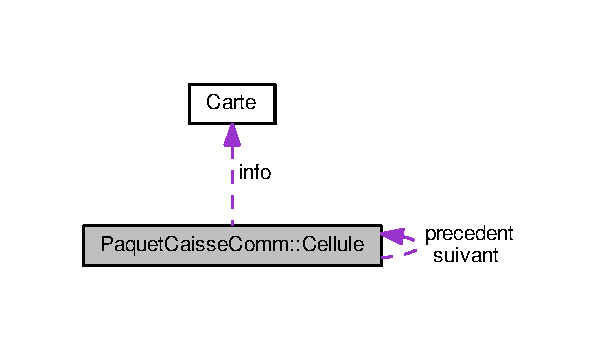
\includegraphics[width=287pt]{structPaquetCaisseComm_1_1Cellule__coll__graph}
\end{center}
\end{figure}
\subsection*{Attributs publics}
\begin{DoxyCompactItemize}
\item 
\hyperlink{classCarte}{Carte} $\ast$ {\bfseries info}\hypertarget{structPaquetCaisseComm_1_1Cellule_a2daf292d52bc4be1c5f9b21e5ca62a70}{}\label{structPaquetCaisseComm_1_1Cellule_a2daf292d52bc4be1c5f9b21e5ca62a70}

\item 
\hyperlink{structPaquetCaisseComm_1_1Cellule}{Cellule} $\ast$ {\bfseries suivant}\hypertarget{structPaquetCaisseComm_1_1Cellule_a95717e932cf65ea9029dad23110de9c7}{}\label{structPaquetCaisseComm_1_1Cellule_a95717e932cf65ea9029dad23110de9c7}

\item 
\hyperlink{structPaquetCaisseComm_1_1Cellule}{Cellule} $\ast$ {\bfseries precedent}\hypertarget{structPaquetCaisseComm_1_1Cellule_af3b6d3460c1e11968739a1f6fb8d845f}{}\label{structPaquetCaisseComm_1_1Cellule_af3b6d3460c1e11968739a1f6fb8d845f}

\end{DoxyCompactItemize}


La documentation de cette structure a été générée à partir du fichier suivant \+:\begin{DoxyCompactItemize}
\item 
src/txt/\hyperlink{PaquetCaisseComm_8h}{Paquet\+Caisse\+Comm.\+h}\end{DoxyCompactItemize}

\hypertarget{structPaquetChance_1_1Cellule}{}\section{Référence de la structure Paquet\+Chance\+:\+:Cellule}
\label{structPaquetChance_1_1Cellule}\index{Paquet\+Chance\+::\+Cellule@{Paquet\+Chance\+::\+Cellule}}


Graphe de collaboration de Paquet\+Chance\+:\+:Cellule\+:
\nopagebreak
\begin{figure}[H]
\begin{center}
\leavevmode
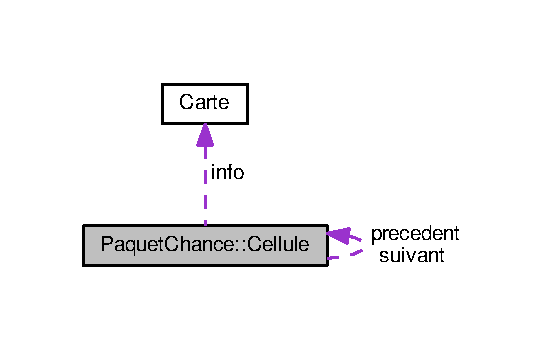
\includegraphics[width=261pt]{structPaquetChance_1_1Cellule__coll__graph}
\end{center}
\end{figure}
\subsection*{Attributs publics}
\begin{DoxyCompactItemize}
\item 
\hyperlink{classCarte}{Carte} $\ast$ {\bfseries info}\hypertarget{structPaquetChance_1_1Cellule_a869e37179243ec2b6056f8a83a8e270e}{}\label{structPaquetChance_1_1Cellule_a869e37179243ec2b6056f8a83a8e270e}

\item 
\hyperlink{structPaquetChance_1_1Cellule}{Cellule} $\ast$ {\bfseries suivant}\hypertarget{structPaquetChance_1_1Cellule_a1e2292d5d6cfbc4377a4a7b0b3a9c6f4}{}\label{structPaquetChance_1_1Cellule_a1e2292d5d6cfbc4377a4a7b0b3a9c6f4}

\item 
\hyperlink{structPaquetChance_1_1Cellule}{Cellule} $\ast$ {\bfseries precedent}\hypertarget{structPaquetChance_1_1Cellule_a7f9c2860bbc80e0be45c3b280cda7730}{}\label{structPaquetChance_1_1Cellule_a7f9c2860bbc80e0be45c3b280cda7730}

\end{DoxyCompactItemize}


La documentation de cette structure a été générée à partir du fichier suivant \+:\begin{DoxyCompactItemize}
\item 
src/txt/\hyperlink{PaquetChance_8h}{Paquet\+Chance.\+h}\end{DoxyCompactItemize}

\hypertarget{classCouleur}{}\section{Référence de la classe Couleur}
\label{classCouleur}\index{Couleur@{Couleur}}


{\ttfamily \#include $<$Couleur.\+h$>$}

\subsection*{Fonctions membres publiques}
\begin{DoxyCompactItemize}
\item 
\hyperlink{classCouleur_a687a457edb08b51dbcd0299bb0b6a882}{Couleur} ()
\begin{DoxyCompactList}\small\item\em Constructeur par defaut de la classe \hyperlink{classCouleur}{Couleur} qui cree une couleur. \end{DoxyCompactList}\item 
\hyperlink{classCouleur_abde5d698dd2ba93ccd9f8fc2c672737d}{Couleur} (unsigned char r, unsigned char v, unsigned char b, string nom)
\begin{DoxyCompactList}\small\item\em Constructeur par parametre de la classe \hyperlink{classCouleur}{Couleur} qui cree une couleur. \end{DoxyCompactList}\item 
bool \hyperlink{classCouleur_a668ffa78890f16427cf7e14dd24ee2f5}{operator==} (\hyperlink{classCouleur}{Couleur} Couleur\+Droite)
\begin{DoxyCompactList}\small\item\em Surcharge de l\textquotesingle{}operateur \char`\"{}==\char`\"{}. \end{DoxyCompactList}\item 
\hyperlink{classCouleur}{Couleur} \& \hyperlink{classCouleur_a9d7642de6177a296f44ad70a8724523c}{operator=} (\hyperlink{classCouleur}{Couleur} Couleur\+Droite)
\begin{DoxyCompactList}\small\item\em Surcharge de l\textquotesingle{}operateur \char`\"{}=\char`\"{}. \end{DoxyCompactList}\item 
unsigned char \hyperlink{classCouleur_a59a0b12ab9cdbff4e2619d97e4cedb97}{get\+Rouge} ()
\begin{DoxyCompactList}\small\item\em obtenir le taux de rouge d\textquotesingle{}une couleur \end{DoxyCompactList}\item 
unsigned char \hyperlink{classCouleur_a165899bdcc10fa60c10eed596ebcb682}{get\+Vert} ()
\begin{DoxyCompactList}\small\item\em obtenir le taux de vert d\textquotesingle{}une couleur \end{DoxyCompactList}\item 
unsigned char \hyperlink{classCouleur_aef20822658bc4a2fd3756b8ed15e02b7}{get\+Bleu} ()
\begin{DoxyCompactList}\small\item\em obtenir le taux de bleu d\textquotesingle{}une couleur \end{DoxyCompactList}\item 
string \hyperlink{classCouleur_a28d35bd6349451ced6b27b06d2a4d429}{get\+Nom\+Couleur} ()
\begin{DoxyCompactList}\small\item\em obtenir le nom d\textquotesingle{}une couleur \end{DoxyCompactList}\item 
void \hyperlink{classCouleur_a8cc9d92d1bf32803c04f5e4ebf314ab4}{set\+Rouge} (unsigned char rouge)
\begin{DoxyCompactList}\small\item\em modifie le taux de rouge d\textquotesingle{}une couleur \end{DoxyCompactList}\item 
void \hyperlink{classCouleur_a7b147a8bf7661866053918c2d4d3cf60}{set\+Vert} (unsigned char vert)
\begin{DoxyCompactList}\small\item\em modifie le taux de vert d\textquotesingle{}une couleur \end{DoxyCompactList}\item 
void \hyperlink{classCouleur_a639e3e3a6b86ed8e2e9ab0e73bff23fe}{set\+Bleu} (unsigned char bleu)
\begin{DoxyCompactList}\small\item\em modifie le taux de bleu d\textquotesingle{}une couleur \end{DoxyCompactList}\item 
void \hyperlink{classCouleur_a92ac934fb56448af9d2ddba17e23ec13}{set\+Nom\+Couleur} (string nom)
\begin{DoxyCompactList}\small\item\em modifie le nom d\textquotesingle{}une couleur \end{DoxyCompactList}\end{DoxyCompactItemize}


\subsection{Description détaillée}
la classe qui permet de generer une case 

\subsection{Documentation des constructeurs et destructeur}
\index{Couleur@{Couleur}!Couleur@{Couleur}}
\index{Couleur@{Couleur}!Couleur@{Couleur}}
\subsubsection[{\texorpdfstring{Couleur()}{Couleur()}}]{\setlength{\rightskip}{0pt plus 5cm}Couleur\+::\+Couleur (
\begin{DoxyParamCaption}
{}
\end{DoxyParamCaption}
)}\hypertarget{classCouleur_a687a457edb08b51dbcd0299bb0b6a882}{}\label{classCouleur_a687a457edb08b51dbcd0299bb0b6a882}


Constructeur par defaut de la classe \hyperlink{classCouleur}{Couleur} qui cree une couleur. 


\begin{DoxyParams}{Paramètres}
{\em pas} & d\textquotesingle{}argument \\
\hline
\end{DoxyParams}
\begin{DoxyReturn}{Renvoie}
retourne une couleur 
\end{DoxyReturn}
\index{Couleur@{Couleur}!Couleur@{Couleur}}
\index{Couleur@{Couleur}!Couleur@{Couleur}}
\subsubsection[{\texorpdfstring{Couleur(unsigned char r, unsigned char v, unsigned char b, string nom)}{Couleur(unsigned char r, unsigned char v, unsigned char b, string nom)}}]{\setlength{\rightskip}{0pt plus 5cm}Couleur\+::\+Couleur (
\begin{DoxyParamCaption}
\item[{unsigned char}]{rouge, }
\item[{unsigned char}]{vert, }
\item[{unsigned char}]{bleu, }
\item[{string}]{nom}
\end{DoxyParamCaption}
)}\hypertarget{classCouleur_abde5d698dd2ba93ccd9f8fc2c672737d}{}\label{classCouleur_abde5d698dd2ba93ccd9f8fc2c672737d}


Constructeur par parametre de la classe \hyperlink{classCouleur}{Couleur} qui cree une couleur. 


\begin{DoxyParams}{Paramètres}
{\em rouge} & chaine de caractere(unsigned char), vert\+: chaine de caractere(unsigned char), bleu\+: chaine de caractere(unsigned char), nom\+: chaine de caractere \\
\hline
\end{DoxyParams}
\begin{DoxyReturn}{Renvoie}
retourne une couleur 
\end{DoxyReturn}


\subsection{Documentation des fonctions membres}
\index{Couleur@{Couleur}!get\+Bleu@{get\+Bleu}}
\index{get\+Bleu@{get\+Bleu}!Couleur@{Couleur}}
\subsubsection[{\texorpdfstring{get\+Bleu()}{getBleu()}}]{\setlength{\rightskip}{0pt plus 5cm}unsigned char Couleur\+::get\+Bleu (
\begin{DoxyParamCaption}
{}
\end{DoxyParamCaption}
)}\hypertarget{classCouleur_aef20822658bc4a2fd3756b8ed15e02b7}{}\label{classCouleur_aef20822658bc4a2fd3756b8ed15e02b7}


obtenir le taux de bleu d\textquotesingle{}une couleur 


\begin{DoxyParams}{Paramètres}
{\em pas} & d\textquotesingle{}argument \\
\hline
\end{DoxyParams}
\begin{DoxyReturn}{Renvoie}
retourne une chaine de caractere (unsigned char) 
\end{DoxyReturn}
\index{Couleur@{Couleur}!get\+Nom\+Couleur@{get\+Nom\+Couleur}}
\index{get\+Nom\+Couleur@{get\+Nom\+Couleur}!Couleur@{Couleur}}
\subsubsection[{\texorpdfstring{get\+Nom\+Couleur()}{getNomCouleur()}}]{\setlength{\rightskip}{0pt plus 5cm}string Couleur\+::get\+Nom\+Couleur (
\begin{DoxyParamCaption}
{}
\end{DoxyParamCaption}
)}\hypertarget{classCouleur_a28d35bd6349451ced6b27b06d2a4d429}{}\label{classCouleur_a28d35bd6349451ced6b27b06d2a4d429}


obtenir le nom d\textquotesingle{}une couleur 


\begin{DoxyParams}{Paramètres}
{\em pas} & d\textquotesingle{}argument \\
\hline
\end{DoxyParams}
\begin{DoxyReturn}{Renvoie}
retourne une chaine de caractere 
\end{DoxyReturn}
\index{Couleur@{Couleur}!get\+Rouge@{get\+Rouge}}
\index{get\+Rouge@{get\+Rouge}!Couleur@{Couleur}}
\subsubsection[{\texorpdfstring{get\+Rouge()}{getRouge()}}]{\setlength{\rightskip}{0pt plus 5cm}unsigned char Couleur\+::get\+Rouge (
\begin{DoxyParamCaption}
{}
\end{DoxyParamCaption}
)}\hypertarget{classCouleur_a59a0b12ab9cdbff4e2619d97e4cedb97}{}\label{classCouleur_a59a0b12ab9cdbff4e2619d97e4cedb97}


obtenir le taux de rouge d\textquotesingle{}une couleur 


\begin{DoxyParams}{Paramètres}
{\em pas} & d\textquotesingle{}argument \\
\hline
\end{DoxyParams}
\begin{DoxyReturn}{Renvoie}
retourne une chaine de caractere (unsigned char) 
\end{DoxyReturn}
\index{Couleur@{Couleur}!get\+Vert@{get\+Vert}}
\index{get\+Vert@{get\+Vert}!Couleur@{Couleur}}
\subsubsection[{\texorpdfstring{get\+Vert()}{getVert()}}]{\setlength{\rightskip}{0pt plus 5cm}unsigned char Couleur\+::get\+Vert (
\begin{DoxyParamCaption}
{}
\end{DoxyParamCaption}
)}\hypertarget{classCouleur_a165899bdcc10fa60c10eed596ebcb682}{}\label{classCouleur_a165899bdcc10fa60c10eed596ebcb682}


obtenir le taux de vert d\textquotesingle{}une couleur 


\begin{DoxyParams}{Paramètres}
{\em pas} & d\textquotesingle{}argument \\
\hline
\end{DoxyParams}
\begin{DoxyReturn}{Renvoie}
retourne une chaine de caractere (unsigned char) 
\end{DoxyReturn}
\index{Couleur@{Couleur}!operator=@{operator=}}
\index{operator=@{operator=}!Couleur@{Couleur}}
\subsubsection[{\texorpdfstring{operator=(\+Couleur Couleur\+Droite)}{operator=(Couleur CouleurDroite)}}]{\setlength{\rightskip}{0pt plus 5cm}{\bf Couleur} \& Couleur\+::operator= (
\begin{DoxyParamCaption}
\item[{{\bf Couleur}}]{Couleur\+Droite}
\end{DoxyParamCaption}
)}\hypertarget{classCouleur_a9d7642de6177a296f44ad70a8724523c}{}\label{classCouleur_a9d7642de6177a296f44ad70a8724523c}


Surcharge de l\textquotesingle{}operateur \char`\"{}=\char`\"{}. 


\begin{DoxyParams}{Paramètres}
{\em Couleur\+Droite} & \hyperlink{classCouleur}{Couleur} \\
\hline
\end{DoxyParams}
\begin{DoxyReturn}{Renvoie}
retourne une couleur 
\end{DoxyReturn}
\index{Couleur@{Couleur}!operator==@{operator==}}
\index{operator==@{operator==}!Couleur@{Couleur}}
\subsubsection[{\texorpdfstring{operator==(\+Couleur Couleur\+Droite)}{operator==(Couleur CouleurDroite)}}]{\setlength{\rightskip}{0pt plus 5cm}bool Couleur\+::operator== (
\begin{DoxyParamCaption}
\item[{{\bf Couleur}}]{Couleur\+Droite}
\end{DoxyParamCaption}
)}\hypertarget{classCouleur_a668ffa78890f16427cf7e14dd24ee2f5}{}\label{classCouleur_a668ffa78890f16427cf7e14dd24ee2f5}


Surcharge de l\textquotesingle{}operateur \char`\"{}==\char`\"{}. 


\begin{DoxyParams}{Paramètres}
{\em Couleur\+Droite} & \hyperlink{classCouleur}{Couleur} \\
\hline
\end{DoxyParams}
\begin{DoxyReturn}{Renvoie}
retourne un booleen 
\end{DoxyReturn}
\index{Couleur@{Couleur}!set\+Bleu@{set\+Bleu}}
\index{set\+Bleu@{set\+Bleu}!Couleur@{Couleur}}
\subsubsection[{\texorpdfstring{set\+Bleu(unsigned char bleu)}{setBleu(unsigned char bleu)}}]{\setlength{\rightskip}{0pt plus 5cm}void Couleur\+::set\+Bleu (
\begin{DoxyParamCaption}
\item[{unsigned char}]{bleu}
\end{DoxyParamCaption}
)}\hypertarget{classCouleur_a639e3e3a6b86ed8e2e9ab0e73bff23fe}{}\label{classCouleur_a639e3e3a6b86ed8e2e9ab0e73bff23fe}


modifie le taux de bleu d\textquotesingle{}une couleur 


\begin{DoxyParams}{Paramètres}
{\em bleu} & chaine de caractere (unsigned char) \\
\hline
\end{DoxyParams}
\begin{DoxyReturn}{Renvoie}
pas de valeur retournee 
\end{DoxyReturn}
\index{Couleur@{Couleur}!set\+Nom\+Couleur@{set\+Nom\+Couleur}}
\index{set\+Nom\+Couleur@{set\+Nom\+Couleur}!Couleur@{Couleur}}
\subsubsection[{\texorpdfstring{set\+Nom\+Couleur(string nom)}{setNomCouleur(string nom)}}]{\setlength{\rightskip}{0pt plus 5cm}void Couleur\+::set\+Nom\+Couleur (
\begin{DoxyParamCaption}
\item[{string}]{nom}
\end{DoxyParamCaption}
)}\hypertarget{classCouleur_a92ac934fb56448af9d2ddba17e23ec13}{}\label{classCouleur_a92ac934fb56448af9d2ddba17e23ec13}


modifie le nom d\textquotesingle{}une couleur 


\begin{DoxyParams}{Paramètres}
{\em bleu} & chaine de caractere (unsigned char) \\
\hline
\end{DoxyParams}
\begin{DoxyReturn}{Renvoie}
pas de valeur retournee 
\end{DoxyReturn}
\index{Couleur@{Couleur}!set\+Rouge@{set\+Rouge}}
\index{set\+Rouge@{set\+Rouge}!Couleur@{Couleur}}
\subsubsection[{\texorpdfstring{set\+Rouge(unsigned char rouge)}{setRouge(unsigned char rouge)}}]{\setlength{\rightskip}{0pt plus 5cm}void Couleur\+::set\+Rouge (
\begin{DoxyParamCaption}
\item[{unsigned char}]{rouge}
\end{DoxyParamCaption}
)}\hypertarget{classCouleur_a8cc9d92d1bf32803c04f5e4ebf314ab4}{}\label{classCouleur_a8cc9d92d1bf32803c04f5e4ebf314ab4}


modifie le taux de rouge d\textquotesingle{}une couleur 


\begin{DoxyParams}{Paramètres}
{\em bleu} & chaine de caractere (unsigned char) \\
\hline
\end{DoxyParams}
\begin{DoxyReturn}{Renvoie}
pas de valeur retournee 
\end{DoxyReturn}
\index{Couleur@{Couleur}!set\+Vert@{set\+Vert}}
\index{set\+Vert@{set\+Vert}!Couleur@{Couleur}}
\subsubsection[{\texorpdfstring{set\+Vert(unsigned char vert)}{setVert(unsigned char vert)}}]{\setlength{\rightskip}{0pt plus 5cm}void Couleur\+::set\+Vert (
\begin{DoxyParamCaption}
\item[{unsigned char}]{vert}
\end{DoxyParamCaption}
)}\hypertarget{classCouleur_a7b147a8bf7661866053918c2d4d3cf60}{}\label{classCouleur_a7b147a8bf7661866053918c2d4d3cf60}


modifie le taux de vert d\textquotesingle{}une couleur 


\begin{DoxyParams}{Paramètres}
{\em bleu} & chaine de caractere (unsigned char) \\
\hline
\end{DoxyParams}
\begin{DoxyReturn}{Renvoie}
pas de valeur retournee 
\end{DoxyReturn}


La documentation de cette classe a été générée à partir des fichiers suivants \+:\begin{DoxyCompactItemize}
\item 
src/txt/\hyperlink{Couleur_8h}{Couleur.\+h}\item 
src/txt/\hyperlink{Couleur_8cpp}{Couleur.\+cpp}\end{DoxyCompactItemize}

\hypertarget{classDe}{}\section{Référence de la classe De}
\label{classDe}\index{De@{De}}


{\ttfamily \#include $<$De.\+h$>$}

\subsection*{Fonctions membres publiques}
\begin{DoxyCompactItemize}
\item 
\hyperlink{classDe_ae6ca2b7255a0bf6dabf745f1f7ca7b40}{De} ()
\begin{DoxyCompactList}\small\item\em Constructeur par defaut de la classe \hyperlink{classDe}{De} qui cree un de. \end{DoxyCompactList}\item 
int \hyperlink{classDe_ae12aeb8230c70da587b5c9087e186871}{Get\+Valeur\+De1} () const 
\begin{DoxyCompactList}\small\item\em obtenir la valeur du premier de \end{DoxyCompactList}\item 
int \hyperlink{classDe_af52bedc1c245414ce82e26a7d5ec10db}{Get\+Valeur\+De2} () const 
\begin{DoxyCompactList}\small\item\em obtenir la valeur du deuxieme de \end{DoxyCompactList}\item 
int \hyperlink{classDe_a2cc67911a29115a7631ca549f4a275a8}{Get\+Serie\+Double} () const 
\begin{DoxyCompactList}\small\item\em obtenir la valeur des des en cas de double \end{DoxyCompactList}\item 
void \hyperlink{classDe_a8b105bd1a2cb4357da368cdf744b058d}{Set\+Valeur\+De1} (int valeur)
\begin{DoxyCompactList}\small\item\em modifier la valeur du premier de \end{DoxyCompactList}\item 
void \hyperlink{classDe_a5f2ec1f957e50b5a1ad677e91835de5e}{Set\+Valeur\+De2} (int valeur)
\begin{DoxyCompactList}\small\item\em modifier la valeur du deuxieme de \end{DoxyCompactList}\item 
void \hyperlink{classDe_ad519be0ea4b6d13f146a2618ad7cecdb}{Set\+Serie\+Double} (int valeur)
\begin{DoxyCompactList}\small\item\em modifier la valeur des des en cas de double \end{DoxyCompactList}\item 
void \hyperlink{classDe_ace08336775f19ffc7b08efd617c22d3e}{Lancer\+De} ()
\begin{DoxyCompactList}\small\item\em la fonction genere aleatoirement deux valeurs pour les deux des \end{DoxyCompactList}\end{DoxyCompactItemize}


\subsection{Description détaillée}
la classe qui permet de generer une case 

\subsection{Documentation des constructeurs et destructeur}
\index{De@{De}!De@{De}}
\index{De@{De}!De@{De}}
\subsubsection[{\texorpdfstring{De()}{De()}}]{\setlength{\rightskip}{0pt plus 5cm}De\+::\+De (
\begin{DoxyParamCaption}
{}
\end{DoxyParamCaption}
)}\hypertarget{classDe_ae6ca2b7255a0bf6dabf745f1f7ca7b40}{}\label{classDe_ae6ca2b7255a0bf6dabf745f1f7ca7b40}


Constructeur par defaut de la classe \hyperlink{classDe}{De} qui cree un de. 


\begin{DoxyParams}{Paramètres}
{\em pas} & d\textquotesingle{}argument \\
\hline
\end{DoxyParams}
\begin{DoxyReturn}{Renvoie}
retourne un de 
\end{DoxyReturn}


\subsection{Documentation des fonctions membres}
\index{De@{De}!Get\+Serie\+Double@{Get\+Serie\+Double}}
\index{Get\+Serie\+Double@{Get\+Serie\+Double}!De@{De}}
\subsubsection[{\texorpdfstring{Get\+Serie\+Double() const }{GetSerieDouble() const }}]{\setlength{\rightskip}{0pt plus 5cm}int De\+::\+Get\+Serie\+Double (
\begin{DoxyParamCaption}
{}
\end{DoxyParamCaption}
) const}\hypertarget{classDe_a2cc67911a29115a7631ca549f4a275a8}{}\label{classDe_a2cc67911a29115a7631ca549f4a275a8}


obtenir la valeur des des en cas de double 


\begin{DoxyParams}{Paramètres}
{\em pas} & d\textquotesingle{}argument \\
\hline
\end{DoxyParams}
\begin{DoxyReturn}{Renvoie}
retourne un entier 
\end{DoxyReturn}
\index{De@{De}!Get\+Valeur\+De1@{Get\+Valeur\+De1}}
\index{Get\+Valeur\+De1@{Get\+Valeur\+De1}!De@{De}}
\subsubsection[{\texorpdfstring{Get\+Valeur\+De1() const }{GetValeurDe1() const }}]{\setlength{\rightskip}{0pt plus 5cm}int De\+::\+Get\+Valeur\+De1 (
\begin{DoxyParamCaption}
{}
\end{DoxyParamCaption}
) const}\hypertarget{classDe_ae12aeb8230c70da587b5c9087e186871}{}\label{classDe_ae12aeb8230c70da587b5c9087e186871}


obtenir la valeur du premier de 


\begin{DoxyParams}{Paramètres}
{\em pas} & d\textquotesingle{}argument \\
\hline
\end{DoxyParams}
\begin{DoxyReturn}{Renvoie}
retourne un entier 
\end{DoxyReturn}
\index{De@{De}!Get\+Valeur\+De2@{Get\+Valeur\+De2}}
\index{Get\+Valeur\+De2@{Get\+Valeur\+De2}!De@{De}}
\subsubsection[{\texorpdfstring{Get\+Valeur\+De2() const }{GetValeurDe2() const }}]{\setlength{\rightskip}{0pt plus 5cm}int De\+::\+Get\+Valeur\+De2 (
\begin{DoxyParamCaption}
{}
\end{DoxyParamCaption}
) const}\hypertarget{classDe_af52bedc1c245414ce82e26a7d5ec10db}{}\label{classDe_af52bedc1c245414ce82e26a7d5ec10db}


obtenir la valeur du deuxieme de 


\begin{DoxyParams}{Paramètres}
{\em pas} & d\textquotesingle{}argument \\
\hline
\end{DoxyParams}
\begin{DoxyReturn}{Renvoie}
retourne un entier 
\end{DoxyReturn}
\index{De@{De}!Lancer\+De@{Lancer\+De}}
\index{Lancer\+De@{Lancer\+De}!De@{De}}
\subsubsection[{\texorpdfstring{Lancer\+De()}{LancerDe()}}]{\setlength{\rightskip}{0pt plus 5cm}void De\+::\+Lancer\+De (
\begin{DoxyParamCaption}
{}
\end{DoxyParamCaption}
)}\hypertarget{classDe_ace08336775f19ffc7b08efd617c22d3e}{}\label{classDe_ace08336775f19ffc7b08efd617c22d3e}


la fonction genere aleatoirement deux valeurs pour les deux des 


\begin{DoxyParams}{Paramètres}
{\em pas} & d\textquotesingle{}argument \\
\hline
\end{DoxyParams}
\begin{DoxyReturn}{Renvoie}
pas de valeur retournee 
\end{DoxyReturn}
\index{De@{De}!Set\+Serie\+Double@{Set\+Serie\+Double}}
\index{Set\+Serie\+Double@{Set\+Serie\+Double}!De@{De}}
\subsubsection[{\texorpdfstring{Set\+Serie\+Double(int valeur)}{SetSerieDouble(int valeur)}}]{\setlength{\rightskip}{0pt plus 5cm}void De\+::\+Set\+Serie\+Double (
\begin{DoxyParamCaption}
\item[{int}]{valeur}
\end{DoxyParamCaption}
)}\hypertarget{classDe_ad519be0ea4b6d13f146a2618ad7cecdb}{}\label{classDe_ad519be0ea4b6d13f146a2618ad7cecdb}


modifier la valeur des des en cas de double 


\begin{DoxyParams}{Paramètres}
{\em valeur} & entier \\
\hline
\end{DoxyParams}
\begin{DoxyReturn}{Renvoie}
pas de valeur retournee 
\end{DoxyReturn}
\index{De@{De}!Set\+Valeur\+De1@{Set\+Valeur\+De1}}
\index{Set\+Valeur\+De1@{Set\+Valeur\+De1}!De@{De}}
\subsubsection[{\texorpdfstring{Set\+Valeur\+De1(int valeur)}{SetValeurDe1(int valeur)}}]{\setlength{\rightskip}{0pt plus 5cm}void De\+::\+Set\+Valeur\+De1 (
\begin{DoxyParamCaption}
\item[{int}]{valeur}
\end{DoxyParamCaption}
)}\hypertarget{classDe_a8b105bd1a2cb4357da368cdf744b058d}{}\label{classDe_a8b105bd1a2cb4357da368cdf744b058d}


modifier la valeur du premier de 


\begin{DoxyParams}{Paramètres}
{\em valeur} & entier \\
\hline
\end{DoxyParams}
\begin{DoxyReturn}{Renvoie}
pas de valeur retournee 
\end{DoxyReturn}
\index{De@{De}!Set\+Valeur\+De2@{Set\+Valeur\+De2}}
\index{Set\+Valeur\+De2@{Set\+Valeur\+De2}!De@{De}}
\subsubsection[{\texorpdfstring{Set\+Valeur\+De2(int valeur)}{SetValeurDe2(int valeur)}}]{\setlength{\rightskip}{0pt plus 5cm}void De\+::\+Set\+Valeur\+De2 (
\begin{DoxyParamCaption}
\item[{int}]{valeur}
\end{DoxyParamCaption}
)}\hypertarget{classDe_a5f2ec1f957e50b5a1ad677e91835de5e}{}\label{classDe_a5f2ec1f957e50b5a1ad677e91835de5e}


modifier la valeur du deuxieme de 


\begin{DoxyParams}{Paramètres}
{\em valeur} & entier \\
\hline
\end{DoxyParams}
\begin{DoxyReturn}{Renvoie}
pas de valeur retournee 
\end{DoxyReturn}


La documentation de cette classe a été générée à partir des fichiers suivants \+:\begin{DoxyCompactItemize}
\item 
src/txt/\hyperlink{De_8h}{De.\+h}\item 
src/txt/\hyperlink{De_8cpp}{De.\+cpp}\end{DoxyCompactItemize}

\hypertarget{classImage}{}\section{Référence de la classe Image}
\label{classImage}\index{Image@{Image}}


Pour g�rer une image avec S\+D\+L2.  




{\ttfamily \#include $<$sdl\+Jeu.\+h$>$}

\subsection*{Fonctions membres publiques}
\begin{DoxyCompactItemize}
\item 
\hyperlink{classImage_a58edd1c45b4faeb5f789b0d036d02313}{Image} ()
\begin{DoxyCompactList}\small\item\em Constructeur par defaut de la classe \hyperlink{classImage}{Image} qui cree une image. \end{DoxyCompactList}\item 
void \hyperlink{classImage_aa276b5183099671ddeaf8f083068046c}{load\+From\+File} (const char $\ast$filename, S\+D\+L\+\_\+\+Renderer $\ast$renderer)
\begin{DoxyCompactList}\small\item\em charge une image depuis un fichier \end{DoxyCompactList}\item 
void \hyperlink{classImage_a82d6936d466ba0161d8b9cbacf613de5}{draw} (S\+D\+L\+\_\+\+Renderer $\ast$renderer, int x, int y, int w=-\/1, int h=-\/1)
\begin{DoxyCompactList}\small\item\em dessine une image a l\textquotesingle{}ecran \end{DoxyCompactList}\end{DoxyCompactItemize}
\subsection*{Attributs publics}
\begin{DoxyCompactItemize}
\item 
S\+D\+L\+\_\+\+Surface $\ast$ {\bfseries surface}\hypertarget{classImage_ac1d365143f4f5ee59f318977ad6d798b}{}\label{classImage_ac1d365143f4f5ee59f318977ad6d798b}

\item 
S\+D\+L\+\_\+\+Texture $\ast$ {\bfseries texture}\hypertarget{classImage_a4f44588a7d341e02dae82e2de94dfad6}{}\label{classImage_a4f44588a7d341e02dae82e2de94dfad6}

\item 
bool {\bfseries has\+\_\+changed}\hypertarget{classImage_ab4cb83faeecef0cfb2773813c4757b45}{}\label{classImage_ab4cb83faeecef0cfb2773813c4757b45}

\end{DoxyCompactItemize}


\subsection{Description détaillée}
Pour g�rer une image avec S\+D\+L2. 

\subsection{Documentation des constructeurs et destructeur}
\index{Image@{Image}!Image@{Image}}
\index{Image@{Image}!Image@{Image}}
\subsubsection[{\texorpdfstring{Image()}{Image()}}]{\setlength{\rightskip}{0pt plus 5cm}Image\+::\+Image (
\begin{DoxyParamCaption}
{}
\end{DoxyParamCaption}
)}\hypertarget{classImage_a58edd1c45b4faeb5f789b0d036d02313}{}\label{classImage_a58edd1c45b4faeb5f789b0d036d02313}


Constructeur par defaut de la classe \hyperlink{classImage}{Image} qui cree une image. 


\begin{DoxyParams}{Paramètres}
{\em pas} & d\textquotesingle{}argument \\
\hline
\end{DoxyParams}
\begin{DoxyReturn}{Renvoie}
retourne une image 
\end{DoxyReturn}


\subsection{Documentation des fonctions membres}
\index{Image@{Image}!draw@{draw}}
\index{draw@{draw}!Image@{Image}}
\subsubsection[{\texorpdfstring{draw(\+S\+D\+L\+\_\+\+Renderer $\ast$renderer, int x, int y, int w=-\/1, int h=-\/1)}{draw(SDL_Renderer *renderer, int x, int y, int w=-1, int h=-1)}}]{\setlength{\rightskip}{0pt plus 5cm}void Image\+::draw (
\begin{DoxyParamCaption}
\item[{S\+D\+L\+\_\+\+Renderer $\ast$}]{renderer, }
\item[{int}]{x, }
\item[{int}]{y, }
\item[{int}]{w = {\ttfamily -\/1}, }
\item[{int}]{h = {\ttfamily -\/1}}
\end{DoxyParamCaption}
)}\hypertarget{classImage_a82d6936d466ba0161d8b9cbacf613de5}{}\label{classImage_a82d6936d466ba0161d8b9cbacf613de5}


dessine une image a l\textquotesingle{}ecran 


\begin{DoxyParams}{Paramètres}
{\em renderer} & S\+D\+L\+\_\+\+Renderer $\ast$, x\+: int, y\+: int, w\+: int, h\+: int \\
\hline
\end{DoxyParams}
\begin{DoxyReturn}{Renvoie}
pas de valeur retournee 
\end{DoxyReturn}
\index{Image@{Image}!load\+From\+File@{load\+From\+File}}
\index{load\+From\+File@{load\+From\+File}!Image@{Image}}
\subsubsection[{\texorpdfstring{load\+From\+File(const char $\ast$filename, S\+D\+L\+\_\+\+Renderer $\ast$renderer)}{loadFromFile(const char *filename, SDL_Renderer *renderer)}}]{\setlength{\rightskip}{0pt plus 5cm}void Image\+::load\+From\+File (
\begin{DoxyParamCaption}
\item[{const char $\ast$}]{filename, }
\item[{S\+D\+L\+\_\+\+Renderer $\ast$}]{renderer}
\end{DoxyParamCaption}
)}\hypertarget{classImage_aa276b5183099671ddeaf8f083068046c}{}\label{classImage_aa276b5183099671ddeaf8f083068046c}


charge une image depuis un fichier 


\begin{DoxyParams}{Paramètres}
{\em filename} & const char$\ast$, renderer\+: S\+D\+L\+\_\+\+Renderer $\ast$ \\
\hline
\end{DoxyParams}
\begin{DoxyReturn}{Renvoie}
pas de valeur retournee 
\end{DoxyReturn}


La documentation de cette classe a été générée à partir des fichiers suivants \+:\begin{DoxyCompactItemize}
\item 
src/sdl2/\hyperlink{sdlJeu_8h}{sdl\+Jeu.\+h}\item 
src/sdl2/\hyperlink{sdlJeu_8cpp}{sdl\+Jeu.\+cpp}\end{DoxyCompactItemize}

\hypertarget{classJeu}{}\section{Référence de la classe Jeu}
\label{classJeu}\index{Jeu@{Jeu}}


{\ttfamily \#include $<$Jeu.\+h$>$}

\subsection*{Fonctions membres publiques}
\begin{DoxyCompactItemize}
\item 
void \hyperlink{classJeu_a437282d939ce54d7f3e2eeb56dc0fce7}{initialiser\+Jeu} ()
\begin{DoxyCompactList}\small\item\em la fonction cree les cases du plateau, les cartes, et les joueurs \end{DoxyCompactList}\item 
\hyperlink{classJeu_a9cd19e73df169d7f09397be61ba8548c}{$\sim$\+Jeu} ()
\begin{DoxyCompactList}\small\item\em le destructeur de la classe \hyperlink{classJeu}{Jeu} \end{DoxyCompactList}\item 
\hyperlink{classJoueur}{Joueur} \hyperlink{classJeu_a0b91f25bdd13913a49d73f4a4f30fa10}{Get\+Joueur} (int num) const 
\begin{DoxyCompactList}\small\item\em Renvoie un joueur a partir de son numero. \end{DoxyCompactList}\item 
const \hyperlink{classPaquetChance}{Paquet\+Chance} \& {\bfseries Get\+Chance} () const \hypertarget{classJeu_a66c298cd9ce97d8c24fbb4109a880e4c}{}\label{classJeu_a66c298cd9ce97d8c24fbb4109a880e4c}

\item 
const \hyperlink{classPaquetCaisseComm}{Paquet\+Caisse\+Comm} \& {\bfseries Get\+Commu} () const \hypertarget{classJeu_a538b9fc6dc3ccaa6a2adb7be6cb039a3}{}\label{classJeu_a538b9fc6dc3ccaa6a2adb7be6cb039a3}

\item 
const \hyperlink{classDe}{De} \& {\bfseries Get\+De} () const \hypertarget{classJeu_a371fdcc4ce95122aedaa4011f6a84dd8}{}\label{classJeu_a371fdcc4ce95122aedaa4011f6a84dd8}

\item 
int \hyperlink{classJeu_addcdf6347e6c0a409bc385ced6965f56}{get\+Nb\+Joueurs} () const 
\begin{DoxyCompactList}\small\item\em Obtenir le nombre de joueurs. \end{DoxyCompactList}\item 
int \hyperlink{classJeu_ad9afa609474f21234d2c78643dfb4bdc}{Nb\+Joueurs\+Restants} ()
\begin{DoxyCompactList}\small\item\em Renvoie le nombre de joueurs restants (non elimines) \end{DoxyCompactList}\item 
void \hyperlink{classJeu_a3f52f74bdf70e7395c65910ab577ff4d}{Tour} (const \hyperlink{classPlateau}{Plateau} \&p, \hyperlink{classPaquetChance}{Paquet\+Chance} \&chance, \hyperlink{classPaquetCaisseComm}{Paquet\+Caisse\+Comm} \&commu, \hyperlink{classDe}{De} des, \hyperlink{classJoueur}{Joueur} $\ast$joueur)
\begin{DoxyCompactList}\small\item\em Gere les tours entre tous les joueurs, propose les actions possibles et prend en compte leurs reponses. \end{DoxyCompactList}\item 
void {\bfseries Enchere} (\hyperlink{classPropriete}{Propriete} \&\hyperlink{classPropriete}{Propriete})\hypertarget{classJeu_ac2bb145d9a3e0b37686a6167ae8028fa}{}\label{classJeu_ac2bb145d9a3e0b37686a6167ae8028fa}

\item 
void \hyperlink{classJeu_a347c8cfc514cdf3e38a9aed2d9af5619}{Prison} (\hyperlink{classPaquetCaisseComm}{Paquet\+Caisse\+Comm} \&commu, \hyperlink{classPaquetChance}{Paquet\+Chance} \&chance, \hyperlink{classDe}{De} Paire\+De, \hyperlink{classJoueur}{Joueur} $\ast$Prisonnier)
\begin{DoxyCompactList}\small\item\em La procedure qui gere les actions d\textquotesingle{}un joueur actuellement en prison. \end{DoxyCompactList}\item 
void {\bfseries Faillite} (\hyperlink{classJoueur}{Joueur} $\ast$joueur)\hypertarget{classJeu_a92d118fa02f22692a5add86578e8f426}{}\label{classJeu_a92d118fa02f22692a5add86578e8f426}

\end{DoxyCompactItemize}


\subsection{Description détaillée}
la classe qui permet de generer une case 

\subsection{Documentation des constructeurs et destructeur}
\index{Jeu@{Jeu}!````~Jeu@{$\sim$\+Jeu}}
\index{````~Jeu@{$\sim$\+Jeu}!Jeu@{Jeu}}
\subsubsection[{\texorpdfstring{$\sim$\+Jeu()}{~Jeu()}}]{\setlength{\rightskip}{0pt plus 5cm}Jeu\+::$\sim$\+Jeu (
\begin{DoxyParamCaption}
{}
\end{DoxyParamCaption}
)}\hypertarget{classJeu_a9cd19e73df169d7f09397be61ba8548c}{}\label{classJeu_a9cd19e73df169d7f09397be61ba8548c}


le destructeur de la classe \hyperlink{classJeu}{Jeu} 


\begin{DoxyParams}{Paramètres}
{\em pas} & d\textquotesingle{}argument \\
\hline
\end{DoxyParams}
\begin{DoxyReturn}{Renvoie}
pas de valeur retournee 
\end{DoxyReturn}


\subsection{Documentation des fonctions membres}
\index{Jeu@{Jeu}!Get\+Joueur@{Get\+Joueur}}
\index{Get\+Joueur@{Get\+Joueur}!Jeu@{Jeu}}
\subsubsection[{\texorpdfstring{Get\+Joueur(int num) const }{GetJoueur(int num) const }}]{\setlength{\rightskip}{0pt plus 5cm}{\bf Joueur} Jeu\+::\+Get\+Joueur (
\begin{DoxyParamCaption}
\item[{int}]{num}
\end{DoxyParamCaption}
) const}\hypertarget{classJeu_a0b91f25bdd13913a49d73f4a4f30fa10}{}\label{classJeu_a0b91f25bdd13913a49d73f4a4f30fa10}


Renvoie un joueur a partir de son numero. 


\begin{DoxyParams}{Paramètres}
{\em num} & entier \\
\hline
\end{DoxyParams}
\begin{DoxyReturn}{Renvoie}
retourne un booleen 
\end{DoxyReturn}
\index{Jeu@{Jeu}!get\+Nb\+Joueurs@{get\+Nb\+Joueurs}}
\index{get\+Nb\+Joueurs@{get\+Nb\+Joueurs}!Jeu@{Jeu}}
\subsubsection[{\texorpdfstring{get\+Nb\+Joueurs() const }{getNbJoueurs() const }}]{\setlength{\rightskip}{0pt plus 5cm}int Jeu\+::get\+Nb\+Joueurs (
\begin{DoxyParamCaption}
{}
\end{DoxyParamCaption}
) const}\hypertarget{classJeu_addcdf6347e6c0a409bc385ced6965f56}{}\label{classJeu_addcdf6347e6c0a409bc385ced6965f56}


Obtenir le nombre de joueurs. 


\begin{DoxyParams}{Paramètres}
{\em pas} & d\textquotesingle{}argument \\
\hline
\end{DoxyParams}
\begin{DoxyReturn}{Renvoie}
retourne un entier 
\end{DoxyReturn}
\index{Jeu@{Jeu}!initialiser\+Jeu@{initialiser\+Jeu}}
\index{initialiser\+Jeu@{initialiser\+Jeu}!Jeu@{Jeu}}
\subsubsection[{\texorpdfstring{initialiser\+Jeu()}{initialiserJeu()}}]{\setlength{\rightskip}{0pt plus 5cm}void Jeu\+::initialiser\+Jeu (
\begin{DoxyParamCaption}
{}
\end{DoxyParamCaption}
)}\hypertarget{classJeu_a437282d939ce54d7f3e2eeb56dc0fce7}{}\label{classJeu_a437282d939ce54d7f3e2eeb56dc0fce7}


la fonction cree les cases du plateau, les cartes, et les joueurs 


\begin{DoxyParams}{Paramètres}
{\em pas} & d\textquotesingle{}argument \\
\hline
\end{DoxyParams}
\begin{DoxyReturn}{Renvoie}
pas de valeur retournee 
\end{DoxyReturn}
\index{Jeu@{Jeu}!Nb\+Joueurs\+Restants@{Nb\+Joueurs\+Restants}}
\index{Nb\+Joueurs\+Restants@{Nb\+Joueurs\+Restants}!Jeu@{Jeu}}
\subsubsection[{\texorpdfstring{Nb\+Joueurs\+Restants()}{NbJoueursRestants()}}]{\setlength{\rightskip}{0pt plus 5cm}int Jeu\+::\+Nb\+Joueurs\+Restants (
\begin{DoxyParamCaption}
{}
\end{DoxyParamCaption}
)}\hypertarget{classJeu_ad9afa609474f21234d2c78643dfb4bdc}{}\label{classJeu_ad9afa609474f21234d2c78643dfb4bdc}


Renvoie le nombre de joueurs restants (non elimines) 


\begin{DoxyParams}{Paramètres}
{\em pas} & d\textquotesingle{}argument \\
\hline
\end{DoxyParams}
\begin{DoxyReturn}{Renvoie}
retourne un entier 
\end{DoxyReturn}
\index{Jeu@{Jeu}!Prison@{Prison}}
\index{Prison@{Prison}!Jeu@{Jeu}}
\subsubsection[{\texorpdfstring{Prison(\+Paquet\+Caisse\+Comm \&commu, Paquet\+Chance \&chance, De Paire\+De, Joueur $\ast$\+Prisonnier)}{Prison(PaquetCaisseComm &commu, PaquetChance &chance, De PaireDe, Joueur *Prisonnier)}}]{\setlength{\rightskip}{0pt plus 5cm}void Jeu\+::\+Prison (
\begin{DoxyParamCaption}
\item[{{\bf Paquet\+Caisse\+Comm} \&}]{commu, }
\item[{{\bf Paquet\+Chance} \&}]{chance, }
\item[{{\bf De}}]{Paire\+De, }
\item[{{\bf Joueur} $\ast$}]{Prisonnier}
\end{DoxyParamCaption}
)}\hypertarget{classJeu_a347c8cfc514cdf3e38a9aed2d9af5619}{}\label{classJeu_a347c8cfc514cdf3e38a9aed2d9af5619}


La procedure qui gere les actions d\textquotesingle{}un joueur actuellement en prison. 


\begin{DoxyParams}{Paramètres}
{\em commu} & \hyperlink{classPaquetCaisseComm}{Paquet\+Caisse\+Comm}, chance\+: \hyperlink{classPaquetChance}{Paquet\+Chance}, Paire\+De\+: \hyperlink{classDe}{De}, Prisonnier\+: \hyperlink{classJoueur}{Joueur} \\
\hline
\end{DoxyParams}
\begin{DoxyReturn}{Renvoie}
pas de valeur retournee 
\end{DoxyReturn}
\index{Jeu@{Jeu}!Tour@{Tour}}
\index{Tour@{Tour}!Jeu@{Jeu}}
\subsubsection[{\texorpdfstring{Tour(const Plateau \&p, Paquet\+Chance \&chance, Paquet\+Caisse\+Comm \&commu, De des, Joueur $\ast$joueur)}{Tour(const Plateau &p, PaquetChance &chance, PaquetCaisseComm &commu, De des, Joueur *joueur)}}]{\setlength{\rightskip}{0pt plus 5cm}void Jeu\+::\+Tour (
\begin{DoxyParamCaption}
\item[{const {\bf Plateau} \&}]{p, }
\item[{{\bf Paquet\+Chance} \&}]{chance, }
\item[{{\bf Paquet\+Caisse\+Comm} \&}]{commu, }
\item[{{\bf De}}]{des, }
\item[{{\bf Joueur} $\ast$}]{joueur}
\end{DoxyParamCaption}
)}\hypertarget{classJeu_a3f52f74bdf70e7395c65910ab577ff4d}{}\label{classJeu_a3f52f74bdf70e7395c65910ab577ff4d}


Gere les tours entre tous les joueurs, propose les actions possibles et prend en compte leurs reponses. 


\begin{DoxyParams}{Paramètres}
{\em p} & \hyperlink{classPlateau}{Plateau}, chance\+: \hyperlink{classPaquetChance}{Paquet\+Chance}, commu\+: \hyperlink{classPaquetCaisseComm}{Paquet\+Caisse\+Comm}, des\+: \hyperlink{classDe}{De}, joueur\+: \hyperlink{classJoueur}{Joueur} \\
\hline
\end{DoxyParams}
\begin{DoxyReturn}{Renvoie}
pas de valeur retournee 
\end{DoxyReturn}


La documentation de cette classe a été générée à partir des fichiers suivants \+:\begin{DoxyCompactItemize}
\item 
src/txt/\hyperlink{Jeu_8h}{Jeu.\+h}\item 
src/txt/\hyperlink{Jeu_8cpp}{Jeu.\+cpp}\end{DoxyCompactItemize}

\hypertarget{classJoueur}{}\section{Référence de la classe Joueur}
\label{classJoueur}\index{Joueur@{Joueur}}


{\ttfamily \#include $<$Joueur.\+h$>$}

\subsection*{Fonctions membres publiques}
\begin{DoxyCompactItemize}
\item 
\hyperlink{classJoueur_add6c98be3020651d84f6d75ccc1d867e}{Joueur} ()
\begin{DoxyCompactList}\small\item\em constructeur par defaut de joueur \end{DoxyCompactList}\item 
\hyperlink{classJoueur_a6b021071dbc36373e27aeefe46b2f3a5}{Joueur} (string Nom, int Numero, const \hyperlink{classCouleur}{Couleur} \&couleur\+Joueur1, const \hyperlink{classCouleur}{Couleur} \&couleur\+Joueur2, const \hyperlink{classCouleur}{Couleur} \&couleur\+Joueur3, const \hyperlink{classCouleur}{Couleur} \&couleur\+Joueur4)
\begin{DoxyCompactList}\small\item\em constructeur par parametre de joueur \end{DoxyCompactList}\item 
\hyperlink{classJoueur}{Joueur} \& \hyperlink{classJoueur_a0a90bcc7315b9756bd7326a3576e03e2}{operator=} (\hyperlink{classJoueur}{Joueur} Joueur\+Droite)
\begin{DoxyCompactList}\small\item\em surcharge de l\textquotesingle{}operateur \char`\"{}=\char`\"{} entre deux joueurs \end{DoxyCompactList}\item 
string \hyperlink{classJoueur_a73a200ab69c2d527a63140e1cf03a5a6}{get\+Nom\+Joueur} () const 
\begin{DoxyCompactList}\small\item\em obtenir le nom d\textquotesingle{}un joueur \end{DoxyCompactList}\item 
int \hyperlink{classJoueur_ae786e53b4e6f69cac8469e03eae0ae8e}{get\+Numero\+Joueur} () const 
\begin{DoxyCompactList}\small\item\em obtenir le numero d\textquotesingle{}un joueur \end{DoxyCompactList}\item 
int \hyperlink{classJoueur_a4fda33fe1f3ee3c79441db3aa108351a}{get\+Cagnotte\+Joueur} () const 
\begin{DoxyCompactList}\small\item\em obtenir la cagnotte d\textquotesingle{}un joueur (l\textquotesingle{}argent qu\textquotesingle{}il a en reserve) \end{DoxyCompactList}\item 
Tableau\+Dynamique \hyperlink{classJoueur_a2526f4cea8724f3ea6b6433a7c5d6737}{get\+Liste\+Proprietes\+Joueur} () const 
\begin{DoxyCompactList}\small\item\em obtenir la liste des proprietes d\textquotesingle{}un joueur \end{DoxyCompactList}\item 
int \hyperlink{classJoueur_aba03f85caafa2ab3ce52d3769845c972}{get\+Position\+Joueur} () const 
\begin{DoxyCompactList}\small\item\em obtenir la position d\textquotesingle{}un joueur \end{DoxyCompactList}\item 
\hyperlink{classCouleur}{Couleur} \hyperlink{classJoueur_abfac9cbad12a4bb882156e75dbbad07f}{get\+Couleur\+Joueur} () const 
\begin{DoxyCompactList}\small\item\em obtenir la couleur d\textquotesingle{}un joueur \end{DoxyCompactList}\item 
int \hyperlink{classJoueur_a9e1ae8232cf4d458c81bcde1cf6cac9d}{get\+Nb\+Carte\+Libre\+Prison} () const 
\begin{DoxyCompactList}\small\item\em obtenir le nombre de cartes \char`\"{}libere de prison\char`\"{} d\textquotesingle{}un joueur \end{DoxyCompactList}\item 
bool \hyperlink{classJoueur_a50562fb939c041ace1822b49cdf5fb1c}{get\+En\+Prison} () const 
\begin{DoxyCompactList}\small\item\em savoir si un joueur est en prison (true) ou non \end{DoxyCompactList}\item 
int \hyperlink{classJoueur_a2875776408bb1a52062ef4403f9ac830}{get\+Nb\+Gare} () const 
\begin{DoxyCompactList}\small\item\em obtenir le nombre de gares d\textquotesingle{}un joueur \end{DoxyCompactList}\item 
int \hyperlink{classJoueur_a92e50af7b49e96d048b75a3114a16f87}{get\+Nb\+Service\+Public} () const 
\begin{DoxyCompactList}\small\item\em obtenir le nombre de services publics d\textquotesingle{}un joueur \end{DoxyCompactList}\item 
bool \hyperlink{classJoueur_a84ce42b1f0c45d71de434de8923318e7}{get\+Encore\+En\+Jeu} () const 
\begin{DoxyCompactList}\small\item\em savoir si un joueur est encore en jeu (true) ou non \end{DoxyCompactList}\item 
int \hyperlink{classJoueur_a2c72233b506965c4725d9941b60a6f6a}{get\+Tour\+Prison} () const 
\begin{DoxyCompactList}\small\item\em obtenir le nombre de tours passes en prison \end{DoxyCompactList}\item 
int \hyperlink{classJoueur_aa9ecdb286b9a2c293fb65f20c169c1c8}{Nb\+Maisons\+Joueur} ()
\begin{DoxyCompactList}\small\item\em obtenir le nombre de maisons d\textquotesingle{}un joueur \end{DoxyCompactList}\item 
int \hyperlink{classJoueur_a42907f6de094a06ced56018c48389d2c}{Nb\+Terrains\+Non\+Hypotheques} ()
\begin{DoxyCompactList}\small\item\em obtenir le nombre de terrains non hypotheques \end{DoxyCompactList}\item 
void \hyperlink{classJoueur_a621f031b62d9a5a2360c7ecbe87963e8}{set\+Nom\+Joueur} (string Nom\+Joueur)
\begin{DoxyCompactList}\small\item\em modifier le nom d\textquotesingle{}un joueur \end{DoxyCompactList}\item 
void \hyperlink{classJoueur_a50820633156f35216a2591f66bab2f7b}{set\+Numero\+Joueur} (int Numero\+Joueur)
\begin{DoxyCompactList}\small\item\em modifier le numero d\textquotesingle{}un joueur \end{DoxyCompactList}\item 
void \hyperlink{classJoueur_a94c32aa334fd5bb3e4ddc96f5b77e1b6}{set\+Cagnotte\+Joueur} (int Cagnotte\+Joueur)
\begin{DoxyCompactList}\small\item\em modifier la cagnotte d\textquotesingle{}un joueur \end{DoxyCompactList}\item 
void \hyperlink{classJoueur_a18c5e436eb68fc995a32c27928e0966a}{set\+Liste\+Proprietes\+Joueur} (\hyperlink{classPropriete}{Propriete} $\ast$e)
\begin{DoxyCompactList}\small\item\em modifier la liste des proprietes d\textquotesingle{}un joueur \end{DoxyCompactList}\item 
void \hyperlink{classJoueur_a16ae199ab457026815521c0cd1e2cd9a}{set\+Position\+Joueur} (int Position\+Joueur)
\begin{DoxyCompactList}\small\item\em modifier la position d\textquotesingle{}un joueur \end{DoxyCompactList}\item 
void \hyperlink{classJoueur_a783f97724d36879e869bbbed3da7df1a}{set\+Couleur\+Joueur} (\hyperlink{classCouleur}{Couleur} Couleur\+Joueur)
\begin{DoxyCompactList}\small\item\em modifier la couleur d\textquotesingle{}un joueur \end{DoxyCompactList}\item 
void \hyperlink{classJoueur_ace62506abea09f7ce35ddf608faf3bf5}{set\+Nb\+Carte\+Libre\+Prison} (int Nb\+Carte\+Libre\+Prison)
\begin{DoxyCompactList}\small\item\em modifier le nombre de cartes \char`\"{}libere de prison\char`\"{} d\textquotesingle{}un joueur \end{DoxyCompactList}\item 
void \hyperlink{classJoueur_a44836db8ee97b5a43d9babd0601c66cf}{set\+En\+Prison} (bool En\+Prison)
\begin{DoxyCompactList}\small\item\em placer un joueur en prison (true) ou l\textquotesingle{}en sortir (false) \end{DoxyCompactList}\item 
void \hyperlink{classJoueur_a1cda809f3eb87380361472541e94ad72}{set\+Nb\+Gare} (int Nb\+Gare)
\begin{DoxyCompactList}\small\item\em modifier le nombre de gares possedees par un joueur \end{DoxyCompactList}\item 
void \hyperlink{classJoueur_ae3d9c066fa56dfbdc93eebd2ffb14f53}{set\+Nb\+Service\+Public} (int Nb\+Service\+Public)
\begin{DoxyCompactList}\small\item\em modifier le nombre de services publics possedes par un joueur \end{DoxyCompactList}\item 
void \hyperlink{classJoueur_a019e018f64e0ece74ce0133e394c9da7}{set\+Encore\+En\+Jeu} (bool x)
\begin{DoxyCompactList}\small\item\em mettre un joueur hors-\/jeu (true) ou non (false) \end{DoxyCompactList}\item 
void \hyperlink{classJoueur_ad27c6fe263fbbcc37f506af658820c66}{set\+Tour\+Prison} (int x)
\begin{DoxyCompactList}\small\item\em modifier le nombre de tours passes en prison \end{DoxyCompactList}\item 
void \hyperlink{classJoueur_a261fbab4596ebac8171122ebab8238d8}{Diminuer\+Argent} (int Somme)
\begin{DoxyCompactList}\small\item\em modifier la cagnotte d\textquotesingle{}un joueur \end{DoxyCompactList}\item 
void \hyperlink{classJoueur_aee0a14e1fcbf775925c2345bb0cc7294}{Augmenter\+Argent} (int Somme)
\begin{DoxyCompactList}\small\item\em modifier la cagnotte d\textquotesingle{}un joueur \end{DoxyCompactList}\item 
void \hyperlink{classJoueur_a88a74f33436855d7068afc8571371f2b}{Avancer} (\hyperlink{classDe}{De} \&Paire\+De)
\begin{DoxyCompactList}\small\item\em faire avancer un joueur au moyen d\textquotesingle{}un lancer de dés \end{DoxyCompactList}\item 
void \hyperlink{classJoueur_ab3f96bf4e675c0424e1910ad0b426fc5}{Avancer\+Case} (int Destination)
\begin{DoxyCompactList}\small\item\em faire avancer un joueur sur une case en particulier \end{DoxyCompactList}\item 
void \hyperlink{classJoueur_a47025d23d2da18cd3fae89a1aa8abffb}{Payer} (int valeur, \hyperlink{classJoueur}{Joueur} \&receveur)
\begin{DoxyCompactList}\small\item\em Oblige un joueur a verser une partie de sa cagnotte a un autre joueur. \end{DoxyCompactList}\item 
void \hyperlink{classJoueur_a3068f8138b55313c8939717b8dcc26bf}{affecter\+Couleur\+Joueur} (\hyperlink{classCouleur}{Couleur} c)
\begin{DoxyCompactList}\small\item\em affecte une couleur a un joueur \end{DoxyCompactList}\item 
void {\bfseries Test\+Regression} ()\hypertarget{classJoueur_aa2bf55ddb18c9addf1418c615f608bec}{}\label{classJoueur_aa2bf55ddb18c9addf1418c615f608bec}

\end{DoxyCompactItemize}


\subsection{Description détaillée}
la classe qui permet de generer une case 

\subsection{Documentation des constructeurs et destructeur}
\index{Joueur@{Joueur}!Joueur@{Joueur}}
\index{Joueur@{Joueur}!Joueur@{Joueur}}
\subsubsection[{\texorpdfstring{Joueur()}{Joueur()}}]{\setlength{\rightskip}{0pt plus 5cm}Joueur\+::\+Joueur (
\begin{DoxyParamCaption}
{}
\end{DoxyParamCaption}
)}\hypertarget{classJoueur_add6c98be3020651d84f6d75ccc1d867e}{}\label{classJoueur_add6c98be3020651d84f6d75ccc1d867e}


constructeur par defaut de joueur 


\begin{DoxyParams}{Paramètres}
{\em pas} & d\textquotesingle{}argument \\
\hline
\end{DoxyParams}
\begin{DoxyReturn}{Renvoie}
retourne un joueur 
\end{DoxyReturn}
\index{Joueur@{Joueur}!Joueur@{Joueur}}
\index{Joueur@{Joueur}!Joueur@{Joueur}}
\subsubsection[{\texorpdfstring{Joueur(string Nom, int Numero, const Couleur \&couleur\+Joueur1, const Couleur \&couleur\+Joueur2, const Couleur \&couleur\+Joueur3, const Couleur \&couleur\+Joueur4)}{Joueur(string Nom, int Numero, const Couleur &couleurJoueur1, const Couleur &couleurJoueur2, const Couleur &couleurJoueur3, const Couleur &couleurJoueur4)}}]{\setlength{\rightskip}{0pt plus 5cm}Joueur\+::\+Joueur (
\begin{DoxyParamCaption}
\item[{string}]{Nom, }
\item[{int}]{Numero, }
\item[{const {\bf Couleur} \&}]{couleur\+Joueur1, }
\item[{const {\bf Couleur} \&}]{couleur\+Joueur2, }
\item[{const {\bf Couleur} \&}]{couleur\+Joueur3, }
\item[{const {\bf Couleur} \&}]{couleur\+Joueur4}
\end{DoxyParamCaption}
)}\hypertarget{classJoueur_a6b021071dbc36373e27aeefe46b2f3a5}{}\label{classJoueur_a6b021071dbc36373e27aeefe46b2f3a5}


constructeur par parametre de joueur 


\begin{DoxyParams}{Paramètres}
{\em Nom} & chaine de caractere, Numero\+: entier, couleur\+Joueur1\+: \hyperlink{classCouleur}{Couleur}, couleur\+Joueur2\+: \hyperlink{classCouleur}{Couleur}, couleur\+Joueur3\+: \hyperlink{classCouleur}{Couleur}, couleur\+Joueur4\+: \hyperlink{classCouleur}{Couleur} \\
\hline
\end{DoxyParams}
\begin{DoxyReturn}{Renvoie}
retourne un joueur 
\end{DoxyReturn}


\subsection{Documentation des fonctions membres}
\index{Joueur@{Joueur}!affecter\+Couleur\+Joueur@{affecter\+Couleur\+Joueur}}
\index{affecter\+Couleur\+Joueur@{affecter\+Couleur\+Joueur}!Joueur@{Joueur}}
\subsubsection[{\texorpdfstring{affecter\+Couleur\+Joueur(\+Couleur c)}{affecterCouleurJoueur(Couleur c)}}]{\setlength{\rightskip}{0pt plus 5cm}void Joueur\+::affecter\+Couleur\+Joueur (
\begin{DoxyParamCaption}
\item[{{\bf Couleur}}]{c}
\end{DoxyParamCaption}
)}\hypertarget{classJoueur_a3068f8138b55313c8939717b8dcc26bf}{}\label{classJoueur_a3068f8138b55313c8939717b8dcc26bf}


affecte une couleur a un joueur 


\begin{DoxyParams}{Paramètres}
{\em c} & \hyperlink{classCouleur}{Couleur} \\
\hline
\end{DoxyParams}
\begin{DoxyReturn}{Renvoie}
pas de valeur retournee 
\end{DoxyReturn}
\index{Joueur@{Joueur}!Augmenter\+Argent@{Augmenter\+Argent}}
\index{Augmenter\+Argent@{Augmenter\+Argent}!Joueur@{Joueur}}
\subsubsection[{\texorpdfstring{Augmenter\+Argent(int Somme)}{AugmenterArgent(int Somme)}}]{\setlength{\rightskip}{0pt plus 5cm}void Joueur\+::\+Augmenter\+Argent (
\begin{DoxyParamCaption}
\item[{int}]{Somme}
\end{DoxyParamCaption}
)}\hypertarget{classJoueur_aee0a14e1fcbf775925c2345bb0cc7294}{}\label{classJoueur_aee0a14e1fcbf775925c2345bb0cc7294}


modifier la cagnotte d\textquotesingle{}un joueur 


\begin{DoxyParams}{Paramètres}
{\em Somme} & entier \\
\hline
\end{DoxyParams}
\begin{DoxyReturn}{Renvoie}
pas de valeur retournee 
\end{DoxyReturn}
\index{Joueur@{Joueur}!Avancer@{Avancer}}
\index{Avancer@{Avancer}!Joueur@{Joueur}}
\subsubsection[{\texorpdfstring{Avancer(\+De \&\+Paire\+De)}{Avancer(De &PaireDe)}}]{\setlength{\rightskip}{0pt plus 5cm}void Joueur\+::\+Avancer (
\begin{DoxyParamCaption}
\item[{{\bf De} \&}]{Paire\+De}
\end{DoxyParamCaption}
)}\hypertarget{classJoueur_a88a74f33436855d7068afc8571371f2b}{}\label{classJoueur_a88a74f33436855d7068afc8571371f2b}


faire avancer un joueur au moyen d\textquotesingle{}un lancer de dés 


\begin{DoxyParams}{Paramètres}
{\em Paire\+De} & entier \\
\hline
\end{DoxyParams}
\begin{DoxyReturn}{Renvoie}
pas de valeur retournee 
\end{DoxyReturn}
\index{Joueur@{Joueur}!Avancer\+Case@{Avancer\+Case}}
\index{Avancer\+Case@{Avancer\+Case}!Joueur@{Joueur}}
\subsubsection[{\texorpdfstring{Avancer\+Case(int Destination)}{AvancerCase(int Destination)}}]{\setlength{\rightskip}{0pt plus 5cm}void Joueur\+::\+Avancer\+Case (
\begin{DoxyParamCaption}
\item[{int}]{Destination}
\end{DoxyParamCaption}
)}\hypertarget{classJoueur_ab3f96bf4e675c0424e1910ad0b426fc5}{}\label{classJoueur_ab3f96bf4e675c0424e1910ad0b426fc5}


faire avancer un joueur sur une case en particulier 


\begin{DoxyParams}{Paramètres}
{\em Destination} & entier \\
\hline
\end{DoxyParams}
\begin{DoxyReturn}{Renvoie}
pas de valeur retournee 
\end{DoxyReturn}
\index{Joueur@{Joueur}!Diminuer\+Argent@{Diminuer\+Argent}}
\index{Diminuer\+Argent@{Diminuer\+Argent}!Joueur@{Joueur}}
\subsubsection[{\texorpdfstring{Diminuer\+Argent(int Somme)}{DiminuerArgent(int Somme)}}]{\setlength{\rightskip}{0pt plus 5cm}void Joueur\+::\+Diminuer\+Argent (
\begin{DoxyParamCaption}
\item[{int}]{Somme}
\end{DoxyParamCaption}
)}\hypertarget{classJoueur_a261fbab4596ebac8171122ebab8238d8}{}\label{classJoueur_a261fbab4596ebac8171122ebab8238d8}


modifier la cagnotte d\textquotesingle{}un joueur 


\begin{DoxyParams}{Paramètres}
{\em Somme} & entier \\
\hline
\end{DoxyParams}
\begin{DoxyReturn}{Renvoie}
pas de valeur retournee 
\end{DoxyReturn}
\index{Joueur@{Joueur}!get\+Cagnotte\+Joueur@{get\+Cagnotte\+Joueur}}
\index{get\+Cagnotte\+Joueur@{get\+Cagnotte\+Joueur}!Joueur@{Joueur}}
\subsubsection[{\texorpdfstring{get\+Cagnotte\+Joueur() const }{getCagnotteJoueur() const }}]{\setlength{\rightskip}{0pt plus 5cm}int Joueur\+::get\+Cagnotte\+Joueur (
\begin{DoxyParamCaption}
{}
\end{DoxyParamCaption}
) const}\hypertarget{classJoueur_a4fda33fe1f3ee3c79441db3aa108351a}{}\label{classJoueur_a4fda33fe1f3ee3c79441db3aa108351a}


obtenir la cagnotte d\textquotesingle{}un joueur (l\textquotesingle{}argent qu\textquotesingle{}il a en reserve) 


\begin{DoxyParams}{Paramètres}
{\em pas} & d\textquotesingle{}argument \\
\hline
\end{DoxyParams}
\begin{DoxyReturn}{Renvoie}
retourne un entier 
\end{DoxyReturn}
\index{Joueur@{Joueur}!get\+Couleur\+Joueur@{get\+Couleur\+Joueur}}
\index{get\+Couleur\+Joueur@{get\+Couleur\+Joueur}!Joueur@{Joueur}}
\subsubsection[{\texorpdfstring{get\+Couleur\+Joueur() const }{getCouleurJoueur() const }}]{\setlength{\rightskip}{0pt plus 5cm}{\bf Couleur} Joueur\+::get\+Couleur\+Joueur (
\begin{DoxyParamCaption}
{}
\end{DoxyParamCaption}
) const}\hypertarget{classJoueur_abfac9cbad12a4bb882156e75dbbad07f}{}\label{classJoueur_abfac9cbad12a4bb882156e75dbbad07f}


obtenir la couleur d\textquotesingle{}un joueur 


\begin{DoxyParams}{Paramètres}
{\em pas} & d\textquotesingle{}argument \\
\hline
\end{DoxyParams}
\begin{DoxyReturn}{Renvoie}
retourne une couleur 
\end{DoxyReturn}
\index{Joueur@{Joueur}!get\+Encore\+En\+Jeu@{get\+Encore\+En\+Jeu}}
\index{get\+Encore\+En\+Jeu@{get\+Encore\+En\+Jeu}!Joueur@{Joueur}}
\subsubsection[{\texorpdfstring{get\+Encore\+En\+Jeu() const }{getEncoreEnJeu() const }}]{\setlength{\rightskip}{0pt plus 5cm}bool Joueur\+::get\+Encore\+En\+Jeu (
\begin{DoxyParamCaption}
{}
\end{DoxyParamCaption}
) const}\hypertarget{classJoueur_a84ce42b1f0c45d71de434de8923318e7}{}\label{classJoueur_a84ce42b1f0c45d71de434de8923318e7}


savoir si un joueur est encore en jeu (true) ou non 


\begin{DoxyParams}{Paramètres}
{\em pas} & d\textquotesingle{}argument \\
\hline
\end{DoxyParams}
\begin{DoxyReturn}{Renvoie}
retourne un booleen 
\end{DoxyReturn}
\index{Joueur@{Joueur}!get\+En\+Prison@{get\+En\+Prison}}
\index{get\+En\+Prison@{get\+En\+Prison}!Joueur@{Joueur}}
\subsubsection[{\texorpdfstring{get\+En\+Prison() const }{getEnPrison() const }}]{\setlength{\rightskip}{0pt plus 5cm}bool Joueur\+::get\+En\+Prison (
\begin{DoxyParamCaption}
{}
\end{DoxyParamCaption}
) const}\hypertarget{classJoueur_a50562fb939c041ace1822b49cdf5fb1c}{}\label{classJoueur_a50562fb939c041ace1822b49cdf5fb1c}


savoir si un joueur est en prison (true) ou non 


\begin{DoxyParams}{Paramètres}
{\em pas} & d\textquotesingle{}argument \\
\hline
\end{DoxyParams}
\begin{DoxyReturn}{Renvoie}
retourne un booleen 
\end{DoxyReturn}
\index{Joueur@{Joueur}!get\+Liste\+Proprietes\+Joueur@{get\+Liste\+Proprietes\+Joueur}}
\index{get\+Liste\+Proprietes\+Joueur@{get\+Liste\+Proprietes\+Joueur}!Joueur@{Joueur}}
\subsubsection[{\texorpdfstring{get\+Liste\+Proprietes\+Joueur() const }{getListeProprietesJoueur() const }}]{\setlength{\rightskip}{0pt plus 5cm}Tableau\+Dynamique Joueur\+::get\+Liste\+Proprietes\+Joueur (
\begin{DoxyParamCaption}
{}
\end{DoxyParamCaption}
) const}\hypertarget{classJoueur_a2526f4cea8724f3ea6b6433a7c5d6737}{}\label{classJoueur_a2526f4cea8724f3ea6b6433a7c5d6737}


obtenir la liste des proprietes d\textquotesingle{}un joueur 


\begin{DoxyParams}{Paramètres}
{\em pas} & d\textquotesingle{}argument \\
\hline
\end{DoxyParams}
\begin{DoxyReturn}{Renvoie}
retourne un tableau dynamique 
\end{DoxyReturn}
\index{Joueur@{Joueur}!get\+Nb\+Carte\+Libre\+Prison@{get\+Nb\+Carte\+Libre\+Prison}}
\index{get\+Nb\+Carte\+Libre\+Prison@{get\+Nb\+Carte\+Libre\+Prison}!Joueur@{Joueur}}
\subsubsection[{\texorpdfstring{get\+Nb\+Carte\+Libre\+Prison() const }{getNbCarteLibrePrison() const }}]{\setlength{\rightskip}{0pt plus 5cm}int Joueur\+::get\+Nb\+Carte\+Libre\+Prison (
\begin{DoxyParamCaption}
{}
\end{DoxyParamCaption}
) const}\hypertarget{classJoueur_a9e1ae8232cf4d458c81bcde1cf6cac9d}{}\label{classJoueur_a9e1ae8232cf4d458c81bcde1cf6cac9d}


obtenir le nombre de cartes \char`\"{}libere de prison\char`\"{} d\textquotesingle{}un joueur 


\begin{DoxyParams}{Paramètres}
{\em pas} & d\textquotesingle{}argument \\
\hline
\end{DoxyParams}
\begin{DoxyReturn}{Renvoie}
retourne un entier 
\end{DoxyReturn}
\index{Joueur@{Joueur}!get\+Nb\+Gare@{get\+Nb\+Gare}}
\index{get\+Nb\+Gare@{get\+Nb\+Gare}!Joueur@{Joueur}}
\subsubsection[{\texorpdfstring{get\+Nb\+Gare() const }{getNbGare() const }}]{\setlength{\rightskip}{0pt plus 5cm}int Joueur\+::get\+Nb\+Gare (
\begin{DoxyParamCaption}
{}
\end{DoxyParamCaption}
) const}\hypertarget{classJoueur_a2875776408bb1a52062ef4403f9ac830}{}\label{classJoueur_a2875776408bb1a52062ef4403f9ac830}


obtenir le nombre de gares d\textquotesingle{}un joueur 


\begin{DoxyParams}{Paramètres}
{\em pas} & d\textquotesingle{}argument \\
\hline
\end{DoxyParams}
\begin{DoxyReturn}{Renvoie}
retourne un entier 
\end{DoxyReturn}
\index{Joueur@{Joueur}!get\+Nb\+Service\+Public@{get\+Nb\+Service\+Public}}
\index{get\+Nb\+Service\+Public@{get\+Nb\+Service\+Public}!Joueur@{Joueur}}
\subsubsection[{\texorpdfstring{get\+Nb\+Service\+Public() const }{getNbServicePublic() const }}]{\setlength{\rightskip}{0pt plus 5cm}int Joueur\+::get\+Nb\+Service\+Public (
\begin{DoxyParamCaption}
{}
\end{DoxyParamCaption}
) const}\hypertarget{classJoueur_a92e50af7b49e96d048b75a3114a16f87}{}\label{classJoueur_a92e50af7b49e96d048b75a3114a16f87}


obtenir le nombre de services publics d\textquotesingle{}un joueur 


\begin{DoxyParams}{Paramètres}
{\em pas} & d\textquotesingle{}argument \\
\hline
\end{DoxyParams}
\begin{DoxyReturn}{Renvoie}
retourne un entier 
\end{DoxyReturn}
\index{Joueur@{Joueur}!get\+Nom\+Joueur@{get\+Nom\+Joueur}}
\index{get\+Nom\+Joueur@{get\+Nom\+Joueur}!Joueur@{Joueur}}
\subsubsection[{\texorpdfstring{get\+Nom\+Joueur() const }{getNomJoueur() const }}]{\setlength{\rightskip}{0pt plus 5cm}string Joueur\+::get\+Nom\+Joueur (
\begin{DoxyParamCaption}
{}
\end{DoxyParamCaption}
) const}\hypertarget{classJoueur_a73a200ab69c2d527a63140e1cf03a5a6}{}\label{classJoueur_a73a200ab69c2d527a63140e1cf03a5a6}


obtenir le nom d\textquotesingle{}un joueur 


\begin{DoxyParams}{Paramètres}
{\em pas} & d\textquotesingle{}argument \\
\hline
\end{DoxyParams}
\begin{DoxyReturn}{Renvoie}
retourne une chaine de caractere 
\end{DoxyReturn}
\index{Joueur@{Joueur}!get\+Numero\+Joueur@{get\+Numero\+Joueur}}
\index{get\+Numero\+Joueur@{get\+Numero\+Joueur}!Joueur@{Joueur}}
\subsubsection[{\texorpdfstring{get\+Numero\+Joueur() const }{getNumeroJoueur() const }}]{\setlength{\rightskip}{0pt plus 5cm}int Joueur\+::get\+Numero\+Joueur (
\begin{DoxyParamCaption}
{}
\end{DoxyParamCaption}
) const}\hypertarget{classJoueur_ae786e53b4e6f69cac8469e03eae0ae8e}{}\label{classJoueur_ae786e53b4e6f69cac8469e03eae0ae8e}


obtenir le numero d\textquotesingle{}un joueur 


\begin{DoxyParams}{Paramètres}
{\em pas} & d\textquotesingle{}argument \\
\hline
\end{DoxyParams}
\begin{DoxyReturn}{Renvoie}
retourne un entier 
\end{DoxyReturn}
\index{Joueur@{Joueur}!get\+Position\+Joueur@{get\+Position\+Joueur}}
\index{get\+Position\+Joueur@{get\+Position\+Joueur}!Joueur@{Joueur}}
\subsubsection[{\texorpdfstring{get\+Position\+Joueur() const }{getPositionJoueur() const }}]{\setlength{\rightskip}{0pt plus 5cm}int Joueur\+::get\+Position\+Joueur (
\begin{DoxyParamCaption}
{}
\end{DoxyParamCaption}
) const}\hypertarget{classJoueur_aba03f85caafa2ab3ce52d3769845c972}{}\label{classJoueur_aba03f85caafa2ab3ce52d3769845c972}


obtenir la position d\textquotesingle{}un joueur 


\begin{DoxyParams}{Paramètres}
{\em pas} & d\textquotesingle{}argument \\
\hline
\end{DoxyParams}
\begin{DoxyReturn}{Renvoie}
retourne un entier 
\end{DoxyReturn}
\index{Joueur@{Joueur}!get\+Tour\+Prison@{get\+Tour\+Prison}}
\index{get\+Tour\+Prison@{get\+Tour\+Prison}!Joueur@{Joueur}}
\subsubsection[{\texorpdfstring{get\+Tour\+Prison() const }{getTourPrison() const }}]{\setlength{\rightskip}{0pt plus 5cm}int Joueur\+::get\+Tour\+Prison (
\begin{DoxyParamCaption}
{}
\end{DoxyParamCaption}
) const}\hypertarget{classJoueur_a2c72233b506965c4725d9941b60a6f6a}{}\label{classJoueur_a2c72233b506965c4725d9941b60a6f6a}


obtenir le nombre de tours passes en prison 


\begin{DoxyParams}{Paramètres}
{\em pas} & d\textquotesingle{}argument \\
\hline
\end{DoxyParams}
\begin{DoxyReturn}{Renvoie}
retourne un entier 
\end{DoxyReturn}
\index{Joueur@{Joueur}!Nb\+Maisons\+Joueur@{Nb\+Maisons\+Joueur}}
\index{Nb\+Maisons\+Joueur@{Nb\+Maisons\+Joueur}!Joueur@{Joueur}}
\subsubsection[{\texorpdfstring{Nb\+Maisons\+Joueur()}{NbMaisonsJoueur()}}]{\setlength{\rightskip}{0pt plus 5cm}int Joueur\+::\+Nb\+Maisons\+Joueur (
\begin{DoxyParamCaption}
{}
\end{DoxyParamCaption}
)}\hypertarget{classJoueur_aa9ecdb286b9a2c293fb65f20c169c1c8}{}\label{classJoueur_aa9ecdb286b9a2c293fb65f20c169c1c8}


obtenir le nombre de maisons d\textquotesingle{}un joueur 


\begin{DoxyParams}{Paramètres}
{\em pas} & d\textquotesingle{}argument \\
\hline
\end{DoxyParams}
\begin{DoxyReturn}{Renvoie}
renvoie un entier 
\end{DoxyReturn}
\index{Joueur@{Joueur}!Nb\+Terrains\+Non\+Hypotheques@{Nb\+Terrains\+Non\+Hypotheques}}
\index{Nb\+Terrains\+Non\+Hypotheques@{Nb\+Terrains\+Non\+Hypotheques}!Joueur@{Joueur}}
\subsubsection[{\texorpdfstring{Nb\+Terrains\+Non\+Hypotheques()}{NbTerrainsNonHypotheques()}}]{\setlength{\rightskip}{0pt plus 5cm}int Joueur\+::\+Nb\+Terrains\+Non\+Hypotheques (
\begin{DoxyParamCaption}
{}
\end{DoxyParamCaption}
)}\hypertarget{classJoueur_a42907f6de094a06ced56018c48389d2c}{}\label{classJoueur_a42907f6de094a06ced56018c48389d2c}


obtenir le nombre de terrains non hypotheques 


\begin{DoxyParams}{Paramètres}
{\em pas} & d\textquotesingle{}argument \\
\hline
\end{DoxyParams}
\begin{DoxyReturn}{Renvoie}
renvoie un entier 
\end{DoxyReturn}
\index{Joueur@{Joueur}!operator=@{operator=}}
\index{operator=@{operator=}!Joueur@{Joueur}}
\subsubsection[{\texorpdfstring{operator=(\+Joueur Joueur\+Droite)}{operator=(Joueur JoueurDroite)}}]{\setlength{\rightskip}{0pt plus 5cm}{\bf Joueur} \& Joueur\+::operator= (
\begin{DoxyParamCaption}
\item[{{\bf Joueur}}]{Joueur\+Droite}
\end{DoxyParamCaption}
)}\hypertarget{classJoueur_a0a90bcc7315b9756bd7326a3576e03e2}{}\label{classJoueur_a0a90bcc7315b9756bd7326a3576e03e2}


surcharge de l\textquotesingle{}operateur \char`\"{}=\char`\"{} entre deux joueurs 


\begin{DoxyParams}{Paramètres}
{\em Joueur\+Droite} & \hyperlink{classJoueur}{Joueur} \\
\hline
\end{DoxyParams}
\begin{DoxyReturn}{Renvoie}
retourne un joueur 
\end{DoxyReturn}
\index{Joueur@{Joueur}!Payer@{Payer}}
\index{Payer@{Payer}!Joueur@{Joueur}}
\subsubsection[{\texorpdfstring{Payer(int valeur, Joueur \&receveur)}{Payer(int valeur, Joueur &receveur)}}]{\setlength{\rightskip}{0pt plus 5cm}void Joueur\+::\+Payer (
\begin{DoxyParamCaption}
\item[{int}]{valeur, }
\item[{{\bf Joueur} \&}]{receveur}
\end{DoxyParamCaption}
)}\hypertarget{classJoueur_a47025d23d2da18cd3fae89a1aa8abffb}{}\label{classJoueur_a47025d23d2da18cd3fae89a1aa8abffb}


Oblige un joueur a verser une partie de sa cagnotte a un autre joueur. 


\begin{DoxyParams}{Paramètres}
{\em valeur} & entier, receveur\+: \hyperlink{classJoueur}{Joueur} \\
\hline
\end{DoxyParams}
\begin{DoxyReturn}{Renvoie}
pas de valeur retournee 
\end{DoxyReturn}
\index{Joueur@{Joueur}!set\+Cagnotte\+Joueur@{set\+Cagnotte\+Joueur}}
\index{set\+Cagnotte\+Joueur@{set\+Cagnotte\+Joueur}!Joueur@{Joueur}}
\subsubsection[{\texorpdfstring{set\+Cagnotte\+Joueur(int Cagnotte\+Joueur)}{setCagnotteJoueur(int CagnotteJoueur)}}]{\setlength{\rightskip}{0pt plus 5cm}void Joueur\+::set\+Cagnotte\+Joueur (
\begin{DoxyParamCaption}
\item[{int}]{Cagnotte}
\end{DoxyParamCaption}
)}\hypertarget{classJoueur_a94c32aa334fd5bb3e4ddc96f5b77e1b6}{}\label{classJoueur_a94c32aa334fd5bb3e4ddc96f5b77e1b6}


modifier la cagnotte d\textquotesingle{}un joueur 


\begin{DoxyParams}{Paramètres}
{\em Cagnotte} & entier \\
\hline
\end{DoxyParams}
\begin{DoxyReturn}{Renvoie}
pas de valeur retournee 
\end{DoxyReturn}
\index{Joueur@{Joueur}!set\+Couleur\+Joueur@{set\+Couleur\+Joueur}}
\index{set\+Couleur\+Joueur@{set\+Couleur\+Joueur}!Joueur@{Joueur}}
\subsubsection[{\texorpdfstring{set\+Couleur\+Joueur(\+Couleur Couleur\+Joueur)}{setCouleurJoueur(Couleur CouleurJoueur)}}]{\setlength{\rightskip}{0pt plus 5cm}void Joueur\+::set\+Couleur\+Joueur (
\begin{DoxyParamCaption}
\item[{{\bf Couleur}}]{CouleurJ}
\end{DoxyParamCaption}
)}\hypertarget{classJoueur_a783f97724d36879e869bbbed3da7df1a}{}\label{classJoueur_a783f97724d36879e869bbbed3da7df1a}


modifier la couleur d\textquotesingle{}un joueur 


\begin{DoxyParams}{Paramètres}
{\em CouleurJ} & \hyperlink{classCouleur}{Couleur} \\
\hline
\end{DoxyParams}
\begin{DoxyReturn}{Renvoie}
pas de valeur retournee 
\end{DoxyReturn}
\index{Joueur@{Joueur}!set\+Encore\+En\+Jeu@{set\+Encore\+En\+Jeu}}
\index{set\+Encore\+En\+Jeu@{set\+Encore\+En\+Jeu}!Joueur@{Joueur}}
\subsubsection[{\texorpdfstring{set\+Encore\+En\+Jeu(bool x)}{setEncoreEnJeu(bool x)}}]{\setlength{\rightskip}{0pt plus 5cm}void Joueur\+::set\+Encore\+En\+Jeu (
\begin{DoxyParamCaption}
\item[{bool}]{x}
\end{DoxyParamCaption}
)}\hypertarget{classJoueur_a019e018f64e0ece74ce0133e394c9da7}{}\label{classJoueur_a019e018f64e0ece74ce0133e394c9da7}


mettre un joueur hors-\/jeu (true) ou non (false) 


\begin{DoxyParams}{Paramètres}
{\em x} & booleen \\
\hline
\end{DoxyParams}
\begin{DoxyReturn}{Renvoie}
pas de valeur retournee 
\end{DoxyReturn}
\index{Joueur@{Joueur}!set\+En\+Prison@{set\+En\+Prison}}
\index{set\+En\+Prison@{set\+En\+Prison}!Joueur@{Joueur}}
\subsubsection[{\texorpdfstring{set\+En\+Prison(bool En\+Prison)}{setEnPrison(bool EnPrison)}}]{\setlength{\rightskip}{0pt plus 5cm}void Joueur\+::set\+En\+Prison (
\begin{DoxyParamCaption}
\item[{bool}]{Prison}
\end{DoxyParamCaption}
)}\hypertarget{classJoueur_a44836db8ee97b5a43d9babd0601c66cf}{}\label{classJoueur_a44836db8ee97b5a43d9babd0601c66cf}


placer un joueur en prison (true) ou l\textquotesingle{}en sortir (false) 


\begin{DoxyParams}{Paramètres}
{\em Prison} & booleen \\
\hline
\end{DoxyParams}
\begin{DoxyReturn}{Renvoie}
pas de valeur retournee 
\end{DoxyReturn}
\index{Joueur@{Joueur}!set\+Liste\+Proprietes\+Joueur@{set\+Liste\+Proprietes\+Joueur}}
\index{set\+Liste\+Proprietes\+Joueur@{set\+Liste\+Proprietes\+Joueur}!Joueur@{Joueur}}
\subsubsection[{\texorpdfstring{set\+Liste\+Proprietes\+Joueur(\+Propriete $\ast$e)}{setListeProprietesJoueur(Propriete *e)}}]{\setlength{\rightskip}{0pt plus 5cm}void Joueur\+::set\+Liste\+Proprietes\+Joueur (
\begin{DoxyParamCaption}
\item[{{\bf Propriete} $\ast$}]{e}
\end{DoxyParamCaption}
)}\hypertarget{classJoueur_a18c5e436eb68fc995a32c27928e0966a}{}\label{classJoueur_a18c5e436eb68fc995a32c27928e0966a}


modifier la liste des proprietes d\textquotesingle{}un joueur 


\begin{DoxyParams}{Paramètres}
{\em e} & \hyperlink{classPropriete}{Propriete} \\
\hline
\end{DoxyParams}
\begin{DoxyReturn}{Renvoie}
pas de valeur retournee 
\end{DoxyReturn}
\index{Joueur@{Joueur}!set\+Nb\+Carte\+Libre\+Prison@{set\+Nb\+Carte\+Libre\+Prison}}
\index{set\+Nb\+Carte\+Libre\+Prison@{set\+Nb\+Carte\+Libre\+Prison}!Joueur@{Joueur}}
\subsubsection[{\texorpdfstring{set\+Nb\+Carte\+Libre\+Prison(int Nb\+Carte\+Libre\+Prison)}{setNbCarteLibrePrison(int NbCarteLibrePrison)}}]{\setlength{\rightskip}{0pt plus 5cm}void Joueur\+::set\+Nb\+Carte\+Libre\+Prison (
\begin{DoxyParamCaption}
\item[{int}]{Nb\+Prison}
\end{DoxyParamCaption}
)}\hypertarget{classJoueur_ace62506abea09f7ce35ddf608faf3bf5}{}\label{classJoueur_ace62506abea09f7ce35ddf608faf3bf5}


modifier le nombre de cartes \char`\"{}libere de prison\char`\"{} d\textquotesingle{}un joueur 


\begin{DoxyParams}{Paramètres}
{\em Nb\+Prison} & entier \\
\hline
\end{DoxyParams}
\begin{DoxyReturn}{Renvoie}
pas de valeur retournee 
\end{DoxyReturn}
\index{Joueur@{Joueur}!set\+Nb\+Gare@{set\+Nb\+Gare}}
\index{set\+Nb\+Gare@{set\+Nb\+Gare}!Joueur@{Joueur}}
\subsubsection[{\texorpdfstring{set\+Nb\+Gare(int Nb\+Gare)}{setNbGare(int NbGare)}}]{\setlength{\rightskip}{0pt plus 5cm}void Joueur\+::set\+Nb\+Gare (
\begin{DoxyParamCaption}
\item[{int}]{Gare}
\end{DoxyParamCaption}
)}\hypertarget{classJoueur_a1cda809f3eb87380361472541e94ad72}{}\label{classJoueur_a1cda809f3eb87380361472541e94ad72}


modifier le nombre de gares possedees par un joueur 


\begin{DoxyParams}{Paramètres}
{\em Gare} & entier \\
\hline
\end{DoxyParams}
\begin{DoxyReturn}{Renvoie}
pas de valeur retournee 
\end{DoxyReturn}
\index{Joueur@{Joueur}!set\+Nb\+Service\+Public@{set\+Nb\+Service\+Public}}
\index{set\+Nb\+Service\+Public@{set\+Nb\+Service\+Public}!Joueur@{Joueur}}
\subsubsection[{\texorpdfstring{set\+Nb\+Service\+Public(int Nb\+Service\+Public)}{setNbServicePublic(int NbServicePublic)}}]{\setlength{\rightskip}{0pt plus 5cm}void Joueur\+::set\+Nb\+Service\+Public (
\begin{DoxyParamCaption}
\item[{int}]{Service\+Public}
\end{DoxyParamCaption}
)}\hypertarget{classJoueur_ae3d9c066fa56dfbdc93eebd2ffb14f53}{}\label{classJoueur_ae3d9c066fa56dfbdc93eebd2ffb14f53}


modifier le nombre de services publics possedes par un joueur 


\begin{DoxyParams}{Paramètres}
{\em Service\+Public} & entier \\
\hline
\end{DoxyParams}
\begin{DoxyReturn}{Renvoie}
pas de valeur retournee 
\end{DoxyReturn}
\index{Joueur@{Joueur}!set\+Nom\+Joueur@{set\+Nom\+Joueur}}
\index{set\+Nom\+Joueur@{set\+Nom\+Joueur}!Joueur@{Joueur}}
\subsubsection[{\texorpdfstring{set\+Nom\+Joueur(string Nom\+Joueur)}{setNomJoueur(string NomJoueur)}}]{\setlength{\rightskip}{0pt plus 5cm}void Joueur\+::set\+Nom\+Joueur (
\begin{DoxyParamCaption}
\item[{string}]{Nom}
\end{DoxyParamCaption}
)}\hypertarget{classJoueur_a621f031b62d9a5a2360c7ecbe87963e8}{}\label{classJoueur_a621f031b62d9a5a2360c7ecbe87963e8}


modifier le nom d\textquotesingle{}un joueur 


\begin{DoxyParams}{Paramètres}
{\em Nom} & chaine de caractere \\
\hline
\end{DoxyParams}
\begin{DoxyReturn}{Renvoie}
pas de valeur retournee 
\end{DoxyReturn}
\index{Joueur@{Joueur}!set\+Numero\+Joueur@{set\+Numero\+Joueur}}
\index{set\+Numero\+Joueur@{set\+Numero\+Joueur}!Joueur@{Joueur}}
\subsubsection[{\texorpdfstring{set\+Numero\+Joueur(int Numero\+Joueur)}{setNumeroJoueur(int NumeroJoueur)}}]{\setlength{\rightskip}{0pt plus 5cm}void Joueur\+::set\+Numero\+Joueur (
\begin{DoxyParamCaption}
\item[{int}]{Numero}
\end{DoxyParamCaption}
)}\hypertarget{classJoueur_a50820633156f35216a2591f66bab2f7b}{}\label{classJoueur_a50820633156f35216a2591f66bab2f7b}


modifier le numero d\textquotesingle{}un joueur 


\begin{DoxyParams}{Paramètres}
{\em Numero} & entier \\
\hline
\end{DoxyParams}
\begin{DoxyReturn}{Renvoie}
pas de valeur retournee 
\end{DoxyReturn}
\index{Joueur@{Joueur}!set\+Position\+Joueur@{set\+Position\+Joueur}}
\index{set\+Position\+Joueur@{set\+Position\+Joueur}!Joueur@{Joueur}}
\subsubsection[{\texorpdfstring{set\+Position\+Joueur(int Position\+Joueur)}{setPositionJoueur(int PositionJoueur)}}]{\setlength{\rightskip}{0pt plus 5cm}void Joueur\+::set\+Position\+Joueur (
\begin{DoxyParamCaption}
\item[{int}]{Position}
\end{DoxyParamCaption}
)}\hypertarget{classJoueur_a16ae199ab457026815521c0cd1e2cd9a}{}\label{classJoueur_a16ae199ab457026815521c0cd1e2cd9a}


modifier la position d\textquotesingle{}un joueur 


\begin{DoxyParams}{Paramètres}
{\em Position} & entier \\
\hline
\end{DoxyParams}
\begin{DoxyReturn}{Renvoie}
pas de valeur retournee 
\end{DoxyReturn}
\index{Joueur@{Joueur}!set\+Tour\+Prison@{set\+Tour\+Prison}}
\index{set\+Tour\+Prison@{set\+Tour\+Prison}!Joueur@{Joueur}}
\subsubsection[{\texorpdfstring{set\+Tour\+Prison(int x)}{setTourPrison(int x)}}]{\setlength{\rightskip}{0pt plus 5cm}void Joueur\+::set\+Tour\+Prison (
\begin{DoxyParamCaption}
\item[{int}]{x}
\end{DoxyParamCaption}
)}\hypertarget{classJoueur_ad27c6fe263fbbcc37f506af658820c66}{}\label{classJoueur_ad27c6fe263fbbcc37f506af658820c66}


modifier le nombre de tours passes en prison 


\begin{DoxyParams}{Paramètres}
{\em x} & entier \\
\hline
\end{DoxyParams}
\begin{DoxyReturn}{Renvoie}
pas de valeur retournee 
\end{DoxyReturn}


La documentation de cette classe a été générée à partir des fichiers suivants \+:\begin{DoxyCompactItemize}
\item 
src/txt/\hyperlink{Joueur_8h}{Joueur.\+h}\item 
src/txt/\hyperlink{Joueur_8cpp}{Joueur.\+cpp}\end{DoxyCompactItemize}

\hypertarget{classPaquetCaisseComm}{}\section{Référence de la classe Paquet\+Caisse\+Comm}
\label{classPaquetCaisseComm}\index{Paquet\+Caisse\+Comm@{Paquet\+Caisse\+Comm}}


{\ttfamily \#include $<$Paquet\+Caisse\+Comm.\+h$>$}



Graphe de collaboration de Paquet\+Caisse\+Comm\+:
\nopagebreak
\begin{figure}[H]
\begin{center}
\leavevmode
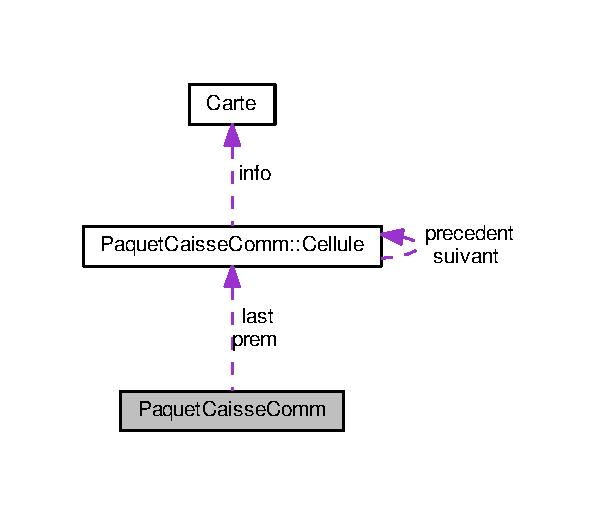
\includegraphics[width=287pt]{classPaquetCaisseComm__coll__graph}
\end{center}
\end{figure}
\subsection*{Classes}
\begin{DoxyCompactItemize}
\item 
struct \hyperlink{structPaquetCaisseComm_1_1Cellule}{Cellule}
\end{DoxyCompactItemize}
\subsection*{Fonctions membres publiques}
\begin{DoxyCompactItemize}
\item 
\hyperlink{classPaquetCaisseComm_aa01ac60f4e3e0ba2ec02402d86432bd8}{Paquet\+Caisse\+Comm} ()
\begin{DoxyCompactList}\small\item\em constructeur par defaut de \hyperlink{classPaquetCaisseComm}{Paquet\+Caisse\+Comm} \end{DoxyCompactList}\item 
\hyperlink{classPaquetCaisseComm_a9ea6dccf1093cdb5807c996745a8ce68}{$\sim$\+Paquet\+Caisse\+Comm} ()
\begin{DoxyCompactList}\small\item\em destructeur de \hyperlink{classPaquetCaisseComm}{Paquet\+Caisse\+Comm} \end{DoxyCompactList}\item 
\hyperlink{classPaquetCaisseComm}{Paquet\+Caisse\+Comm} \& \hyperlink{classPaquetCaisseComm_aca9657c21e06fff1f0ffa3a1030cec27}{operator=} (const \hyperlink{classPaquetCaisseComm}{Paquet\+Caisse\+Comm} \&p)
\begin{DoxyCompactList}\small\item\em surcharge de l\textquotesingle{}operateur \char`\"{}=\char`\"{} entre deux paquets de \char`\"{}caisse communaute\char`\"{} \end{DoxyCompactList}\item 
void \hyperlink{classPaquetCaisseComm_a41f3a14b45c12fa770774c2871a1e257}{vider} ()
\begin{DoxyCompactList}\small\item\em vide la liste \hyperlink{classPaquetCaisseComm}{Paquet\+Caisse\+Comm} de toutes ses cellules (cartes) \end{DoxyCompactList}\item 
bool \hyperlink{classPaquetCaisseComm_a82100c34993a74ad83876a81d8cbd722}{est\+Vide} () const 
\begin{DoxyCompactList}\small\item\em verifie si une file est bien vide (true) ou non (false) \end{DoxyCompactList}\item 
unsigned int \hyperlink{classPaquetCaisseComm_a0ccefaf67a8186a9ff5960eb5b408b22}{nb\+Elements} () const 
\begin{DoxyCompactList}\small\item\em Compte le nombre d\textquotesingle{}elements dans la file. \end{DoxyCompactList}\item 
\hyperlink{classCarte}{Carte} $\ast$ \hyperlink{classPaquetCaisseComm_ac3aa3b696803e1afaf3a978b19c49cd1}{ieme\+Element} (unsigned int indice) const 
\begin{DoxyCompactList}\small\item\em Selectionne la i-\/eme carte de la file. \end{DoxyCompactList}\item 
void \hyperlink{classPaquetCaisseComm_a3754d7aa4b776ea756c48883ae124bf6}{modifier\+Ieme\+Element} (unsigned int indice, \hyperlink{classCarte}{Carte} $\ast$e)
\begin{DoxyCompactList}\small\item\em Remplace le i-\/eme element par une carte passee en parametre. \end{DoxyCompactList}\item 
void \hyperlink{classPaquetCaisseComm_ada42acf9646a98e6fa4231a99c3106ac}{ajouter\+En\+Tete} (\hyperlink{classCarte}{Carte} $\ast$e)
\begin{DoxyCompactList}\small\item\em Ajoute un element passe en parametre au debut de la file. \end{DoxyCompactList}\item 
void \hyperlink{classPaquetCaisseComm_a90365361fe2b32fe7327f5ea081fc859}{ajouter\+En\+Queue} (\hyperlink{classCarte}{Carte} $\ast$e)
\begin{DoxyCompactList}\small\item\em Ajoute un element passe en parametre a la fin de la file. \end{DoxyCompactList}\item 
void \hyperlink{classPaquetCaisseComm_a2327d7c648c57284d7d3d43d497bc707}{supprimer\+Tete} ()
\begin{DoxyCompactList}\small\item\em Supprime le premier element de la file. \end{DoxyCompactList}\item 
void \hyperlink{classPaquetCaisseComm_a7fe35a8526b71bde8c994ecea7c17086}{inserer\+Element} (\hyperlink{classCarte}{Carte} $\ast$e, unsigned int indice)
\begin{DoxyCompactList}\small\item\em Insere une carte a la i-\/eme place de la file. \end{DoxyCompactList}\item 
void \hyperlink{classPaquetCaisseComm_a63bee5d115614b01e31f6adb7ec6059d}{trier} ()
\begin{DoxyCompactList}\small\item\em Trie la file en fonction de l\textquotesingle{}id des cartes. \end{DoxyCompactList}\item 
\hyperlink{classCarte}{Carte} $\ast$ \hyperlink{classPaquetCaisseComm_a672f8287e8e43aad21694d5a26bd7de2}{Piocher\+Carte} ()
\begin{DoxyCompactList}\small\item\em Pioche une carte, execute son effet, et la remet a la fin du paquet. \end{DoxyCompactList}\end{DoxyCompactItemize}
\subsection*{Attributs publics}
\begin{DoxyCompactItemize}
\item 
\hyperlink{structPaquetCaisseComm_1_1Cellule}{Cellule} $\ast$ {\bfseries prem}\hypertarget{classPaquetCaisseComm_a5bf4a1577be9c7b914e6e4c7952d48ab}{}\label{classPaquetCaisseComm_a5bf4a1577be9c7b914e6e4c7952d48ab}

\item 
\hyperlink{structPaquetCaisseComm_1_1Cellule}{Cellule} $\ast$ {\bfseries last}\hypertarget{classPaquetCaisseComm_a9e9398de4eab76c0fa784a1a2be4a6da}{}\label{classPaquetCaisseComm_a9e9398de4eab76c0fa784a1a2be4a6da}

\end{DoxyCompactItemize}


\subsection{Description détaillée}
la classe qui permet de generer une case 

\subsection{Documentation des constructeurs et destructeur}
\index{Paquet\+Caisse\+Comm@{Paquet\+Caisse\+Comm}!Paquet\+Caisse\+Comm@{Paquet\+Caisse\+Comm}}
\index{Paquet\+Caisse\+Comm@{Paquet\+Caisse\+Comm}!Paquet\+Caisse\+Comm@{Paquet\+Caisse\+Comm}}
\subsubsection[{\texorpdfstring{Paquet\+Caisse\+Comm()}{PaquetCaisseComm()}}]{\setlength{\rightskip}{0pt plus 5cm}Paquet\+Caisse\+Comm\+::\+Paquet\+Caisse\+Comm (
\begin{DoxyParamCaption}
{}
\end{DoxyParamCaption}
)}\hypertarget{classPaquetCaisseComm_aa01ac60f4e3e0ba2ec02402d86432bd8}{}\label{classPaquetCaisseComm_aa01ac60f4e3e0ba2ec02402d86432bd8}


constructeur par defaut de \hyperlink{classPaquetCaisseComm}{Paquet\+Caisse\+Comm} 


\begin{DoxyParams}{Paramètres}
{\em pas} & d\textquotesingle{}argument \\
\hline
\end{DoxyParams}
\begin{DoxyReturn}{Renvoie}
retourne une file de cartes \char`\"{}caisse de communaute\char`\"{} 
\end{DoxyReturn}
\index{Paquet\+Caisse\+Comm@{Paquet\+Caisse\+Comm}!````~Paquet\+Caisse\+Comm@{$\sim$\+Paquet\+Caisse\+Comm}}
\index{````~Paquet\+Caisse\+Comm@{$\sim$\+Paquet\+Caisse\+Comm}!Paquet\+Caisse\+Comm@{Paquet\+Caisse\+Comm}}
\subsubsection[{\texorpdfstring{$\sim$\+Paquet\+Caisse\+Comm()}{~PaquetCaisseComm()}}]{\setlength{\rightskip}{0pt plus 5cm}Paquet\+Caisse\+Comm\+::$\sim$\+Paquet\+Caisse\+Comm (
\begin{DoxyParamCaption}
{}
\end{DoxyParamCaption}
)}\hypertarget{classPaquetCaisseComm_a9ea6dccf1093cdb5807c996745a8ce68}{}\label{classPaquetCaisseComm_a9ea6dccf1093cdb5807c996745a8ce68}


destructeur de \hyperlink{classPaquetCaisseComm}{Paquet\+Caisse\+Comm} 


\begin{DoxyParams}{Paramètres}
{\em pas} & d\textquotesingle{}argument \\
\hline
\end{DoxyParams}
\begin{DoxyReturn}{Renvoie}
pas de valeur retournee 
\end{DoxyReturn}


\subsection{Documentation des fonctions membres}
\index{Paquet\+Caisse\+Comm@{Paquet\+Caisse\+Comm}!ajouter\+En\+Queue@{ajouter\+En\+Queue}}
\index{ajouter\+En\+Queue@{ajouter\+En\+Queue}!Paquet\+Caisse\+Comm@{Paquet\+Caisse\+Comm}}
\subsubsection[{\texorpdfstring{ajouter\+En\+Queue(\+Carte $\ast$e)}{ajouterEnQueue(Carte *e)}}]{\setlength{\rightskip}{0pt plus 5cm}void Paquet\+Caisse\+Comm\+::ajouter\+En\+Queue (
\begin{DoxyParamCaption}
\item[{{\bf Carte} $\ast$}]{e}
\end{DoxyParamCaption}
)}\hypertarget{classPaquetCaisseComm_a90365361fe2b32fe7327f5ea081fc859}{}\label{classPaquetCaisseComm_a90365361fe2b32fe7327f5ea081fc859}


Ajoute un element passe en parametre a la fin de la file. 


\begin{DoxyParams}{Paramètres}
{\em $\ast$e} & \hyperlink{classCarte}{Carte} \\
\hline
\end{DoxyParams}
\begin{DoxyReturn}{Renvoie}
pas de valeur retournee 
\end{DoxyReturn}
\index{Paquet\+Caisse\+Comm@{Paquet\+Caisse\+Comm}!ajouter\+En\+Tete@{ajouter\+En\+Tete}}
\index{ajouter\+En\+Tete@{ajouter\+En\+Tete}!Paquet\+Caisse\+Comm@{Paquet\+Caisse\+Comm}}
\subsubsection[{\texorpdfstring{ajouter\+En\+Tete(\+Carte $\ast$e)}{ajouterEnTete(Carte *e)}}]{\setlength{\rightskip}{0pt plus 5cm}void Paquet\+Caisse\+Comm\+::ajouter\+En\+Tete (
\begin{DoxyParamCaption}
\item[{{\bf Carte} $\ast$}]{e}
\end{DoxyParamCaption}
)}\hypertarget{classPaquetCaisseComm_ada42acf9646a98e6fa4231a99c3106ac}{}\label{classPaquetCaisseComm_ada42acf9646a98e6fa4231a99c3106ac}


Ajoute un element passe en parametre au debut de la file. 


\begin{DoxyParams}{Paramètres}
{\em $\ast$e} & \hyperlink{classCarte}{Carte} \\
\hline
\end{DoxyParams}
\begin{DoxyReturn}{Renvoie}
pas de valeur retournee 
\end{DoxyReturn}
\index{Paquet\+Caisse\+Comm@{Paquet\+Caisse\+Comm}!est\+Vide@{est\+Vide}}
\index{est\+Vide@{est\+Vide}!Paquet\+Caisse\+Comm@{Paquet\+Caisse\+Comm}}
\subsubsection[{\texorpdfstring{est\+Vide() const }{estVide() const }}]{\setlength{\rightskip}{0pt plus 5cm}bool Paquet\+Caisse\+Comm\+::est\+Vide (
\begin{DoxyParamCaption}
{}
\end{DoxyParamCaption}
) const}\hypertarget{classPaquetCaisseComm_a82100c34993a74ad83876a81d8cbd722}{}\label{classPaquetCaisseComm_a82100c34993a74ad83876a81d8cbd722}


verifie si une file est bien vide (true) ou non (false) 


\begin{DoxyParams}{Paramètres}
{\em pas} & d\textquotesingle{}argument \\
\hline
\end{DoxyParams}
\begin{DoxyReturn}{Renvoie}
retourne un booleen 
\end{DoxyReturn}
\index{Paquet\+Caisse\+Comm@{Paquet\+Caisse\+Comm}!ieme\+Element@{ieme\+Element}}
\index{ieme\+Element@{ieme\+Element}!Paquet\+Caisse\+Comm@{Paquet\+Caisse\+Comm}}
\subsubsection[{\texorpdfstring{ieme\+Element(unsigned int indice) const }{iemeElement(unsigned int indice) const }}]{\setlength{\rightskip}{0pt plus 5cm}{\bf Carte} $\ast$ Paquet\+Caisse\+Comm\+::ieme\+Element (
\begin{DoxyParamCaption}
\item[{unsigned int}]{i}
\end{DoxyParamCaption}
) const}\hypertarget{classPaquetCaisseComm_ac3aa3b696803e1afaf3a978b19c49cd1}{}\label{classPaquetCaisseComm_ac3aa3b696803e1afaf3a978b19c49cd1}


Selectionne la i-\/eme carte de la file. 


\begin{DoxyParams}{Paramètres}
{\em indice} & entier positif \\
\hline
\end{DoxyParams}
\begin{DoxyReturn}{Renvoie}
retourne une \hyperlink{classCarte}{Carte} 
\end{DoxyReturn}
\index{Paquet\+Caisse\+Comm@{Paquet\+Caisse\+Comm}!inserer\+Element@{inserer\+Element}}
\index{inserer\+Element@{inserer\+Element}!Paquet\+Caisse\+Comm@{Paquet\+Caisse\+Comm}}
\subsubsection[{\texorpdfstring{inserer\+Element(\+Carte $\ast$e, unsigned int indice)}{insererElement(Carte *e, unsigned int indice)}}]{\setlength{\rightskip}{0pt plus 5cm}void Paquet\+Caisse\+Comm\+::inserer\+Element (
\begin{DoxyParamCaption}
\item[{{\bf Carte} $\ast$}]{e, }
\item[{unsigned int}]{position}
\end{DoxyParamCaption}
)}\hypertarget{classPaquetCaisseComm_a7fe35a8526b71bde8c994ecea7c17086}{}\label{classPaquetCaisseComm_a7fe35a8526b71bde8c994ecea7c17086}


Insere une carte a la i-\/eme place de la file. 


\begin{DoxyParams}{Paramètres}
{\em $\ast$e} & \hyperlink{classCarte}{Carte}, indice\+: entier positif \\
\hline
\end{DoxyParams}
\begin{DoxyReturn}{Renvoie}
pas de valeur retournee 
\end{DoxyReturn}
\index{Paquet\+Caisse\+Comm@{Paquet\+Caisse\+Comm}!modifier\+Ieme\+Element@{modifier\+Ieme\+Element}}
\index{modifier\+Ieme\+Element@{modifier\+Ieme\+Element}!Paquet\+Caisse\+Comm@{Paquet\+Caisse\+Comm}}
\subsubsection[{\texorpdfstring{modifier\+Ieme\+Element(unsigned int indice, Carte $\ast$e)}{modifierIemeElement(unsigned int indice, Carte *e)}}]{\setlength{\rightskip}{0pt plus 5cm}void Paquet\+Caisse\+Comm\+::modifier\+Ieme\+Element (
\begin{DoxyParamCaption}
\item[{unsigned int}]{i, }
\item[{{\bf Carte} $\ast$}]{e}
\end{DoxyParamCaption}
)}\hypertarget{classPaquetCaisseComm_a3754d7aa4b776ea756c48883ae124bf6}{}\label{classPaquetCaisseComm_a3754d7aa4b776ea756c48883ae124bf6}


Remplace le i-\/eme element par une carte passee en parametre. 


\begin{DoxyParams}{Paramètres}
{\em indice} & entier positif, $\ast$e\+: \hyperlink{classCarte}{Carte} \\
\hline
\end{DoxyParams}
\begin{DoxyReturn}{Renvoie}
pas de valeur retournee 
\end{DoxyReturn}
\index{Paquet\+Caisse\+Comm@{Paquet\+Caisse\+Comm}!nb\+Elements@{nb\+Elements}}
\index{nb\+Elements@{nb\+Elements}!Paquet\+Caisse\+Comm@{Paquet\+Caisse\+Comm}}
\subsubsection[{\texorpdfstring{nb\+Elements() const }{nbElements() const }}]{\setlength{\rightskip}{0pt plus 5cm}unsigned int Paquet\+Caisse\+Comm\+::nb\+Elements (
\begin{DoxyParamCaption}
{}
\end{DoxyParamCaption}
) const}\hypertarget{classPaquetCaisseComm_a0ccefaf67a8186a9ff5960eb5b408b22}{}\label{classPaquetCaisseComm_a0ccefaf67a8186a9ff5960eb5b408b22}


Compte le nombre d\textquotesingle{}elements dans la file. 


\begin{DoxyParams}{Paramètres}
{\em pas} & d\textquotesingle{}argument \\
\hline
\end{DoxyParams}
\begin{DoxyReturn}{Renvoie}
retourne un entier positif 
\end{DoxyReturn}
\index{Paquet\+Caisse\+Comm@{Paquet\+Caisse\+Comm}!operator=@{operator=}}
\index{operator=@{operator=}!Paquet\+Caisse\+Comm@{Paquet\+Caisse\+Comm}}
\subsubsection[{\texorpdfstring{operator=(const Paquet\+Caisse\+Comm \&p)}{operator=(const PaquetCaisseComm &p)}}]{\setlength{\rightskip}{0pt plus 5cm}{\bf Paquet\+Caisse\+Comm} \& Paquet\+Caisse\+Comm\+::operator= (
\begin{DoxyParamCaption}
\item[{const {\bf Paquet\+Caisse\+Comm} \&}]{l}
\end{DoxyParamCaption}
)}\hypertarget{classPaquetCaisseComm_aca9657c21e06fff1f0ffa3a1030cec27}{}\label{classPaquetCaisseComm_aca9657c21e06fff1f0ffa3a1030cec27}


surcharge de l\textquotesingle{}operateur \char`\"{}=\char`\"{} entre deux paquets de \char`\"{}caisse communaute\char`\"{} 


\begin{DoxyParams}{Paramètres}
{\em p} & \hyperlink{classPaquetCaisseComm}{Paquet\+Caisse\+Comm} \\
\hline
\end{DoxyParams}
\begin{DoxyReturn}{Renvoie}
retourne un paquet de \char`\"{}caisse communaute\char`\"{} 
\end{DoxyReturn}
\index{Paquet\+Caisse\+Comm@{Paquet\+Caisse\+Comm}!Piocher\+Carte@{Piocher\+Carte}}
\index{Piocher\+Carte@{Piocher\+Carte}!Paquet\+Caisse\+Comm@{Paquet\+Caisse\+Comm}}
\subsubsection[{\texorpdfstring{Piocher\+Carte()}{PiocherCarte()}}]{\setlength{\rightskip}{0pt plus 5cm}{\bf Carte} $\ast$ Paquet\+Caisse\+Comm\+::\+Piocher\+Carte (
\begin{DoxyParamCaption}
{}
\end{DoxyParamCaption}
)}\hypertarget{classPaquetCaisseComm_a672f8287e8e43aad21694d5a26bd7de2}{}\label{classPaquetCaisseComm_a672f8287e8e43aad21694d5a26bd7de2}


Pioche une carte, execute son effet, et la remet a la fin du paquet. 


\begin{DoxyParams}{Paramètres}
{\em pas} & d\textquotesingle{}argument \\
\hline
\end{DoxyParams}
\begin{DoxyReturn}{Renvoie}
renvoie une \hyperlink{classCarte}{Carte} 
\end{DoxyReturn}
\index{Paquet\+Caisse\+Comm@{Paquet\+Caisse\+Comm}!supprimer\+Tete@{supprimer\+Tete}}
\index{supprimer\+Tete@{supprimer\+Tete}!Paquet\+Caisse\+Comm@{Paquet\+Caisse\+Comm}}
\subsubsection[{\texorpdfstring{supprimer\+Tete()}{supprimerTete()}}]{\setlength{\rightskip}{0pt plus 5cm}void Paquet\+Caisse\+Comm\+::supprimer\+Tete (
\begin{DoxyParamCaption}
{}
\end{DoxyParamCaption}
)}\hypertarget{classPaquetCaisseComm_a2327d7c648c57284d7d3d43d497bc707}{}\label{classPaquetCaisseComm_a2327d7c648c57284d7d3d43d497bc707}


Supprime le premier element de la file. 


\begin{DoxyParams}{Paramètres}
{\em pas} & d\textquotesingle{}argument \\
\hline
\end{DoxyParams}
\begin{DoxyReturn}{Renvoie}
pas de valeur retournee 
\end{DoxyReturn}
\index{Paquet\+Caisse\+Comm@{Paquet\+Caisse\+Comm}!trier@{trier}}
\index{trier@{trier}!Paquet\+Caisse\+Comm@{Paquet\+Caisse\+Comm}}
\subsubsection[{\texorpdfstring{trier()}{trier()}}]{\setlength{\rightskip}{0pt plus 5cm}void Paquet\+Caisse\+Comm\+::trier (
\begin{DoxyParamCaption}
{}
\end{DoxyParamCaption}
)}\hypertarget{classPaquetCaisseComm_a63bee5d115614b01e31f6adb7ec6059d}{}\label{classPaquetCaisseComm_a63bee5d115614b01e31f6adb7ec6059d}


Trie la file en fonction de l\textquotesingle{}id des cartes. 


\begin{DoxyParams}{Paramètres}
{\em pas} & d\textquotesingle{}argument \\
\hline
\end{DoxyParams}
\begin{DoxyReturn}{Renvoie}
pas de valeur retournee 
\end{DoxyReturn}
\index{Paquet\+Caisse\+Comm@{Paquet\+Caisse\+Comm}!vider@{vider}}
\index{vider@{vider}!Paquet\+Caisse\+Comm@{Paquet\+Caisse\+Comm}}
\subsubsection[{\texorpdfstring{vider()}{vider()}}]{\setlength{\rightskip}{0pt plus 5cm}void Paquet\+Caisse\+Comm\+::vider (
\begin{DoxyParamCaption}
{}
\end{DoxyParamCaption}
)}\hypertarget{classPaquetCaisseComm_a41f3a14b45c12fa770774c2871a1e257}{}\label{classPaquetCaisseComm_a41f3a14b45c12fa770774c2871a1e257}


vide la liste \hyperlink{classPaquetCaisseComm}{Paquet\+Caisse\+Comm} de toutes ses cellules (cartes) 


\begin{DoxyParams}{Paramètres}
{\em pas} & d\textquotesingle{}argument \\
\hline
\end{DoxyParams}
\begin{DoxyReturn}{Renvoie}
pas de valeur retournee 
\end{DoxyReturn}


La documentation de cette classe a été générée à partir des fichiers suivants \+:\begin{DoxyCompactItemize}
\item 
src/txt/\hyperlink{PaquetCaisseComm_8h}{Paquet\+Caisse\+Comm.\+h}\item 
src/txt/\hyperlink{PaquetCaisseComm_8cpp}{Paquet\+Caisse\+Comm.\+cpp}\end{DoxyCompactItemize}

\hypertarget{classPaquetChance}{}\section{Référence de la classe Paquet\+Chance}
\label{classPaquetChance}\index{Paquet\+Chance@{Paquet\+Chance}}


{\ttfamily \#include $<$Paquet\+Chance.\+h$>$}



Graphe de collaboration de Paquet\+Chance\+:
\nopagebreak
\begin{figure}[H]
\begin{center}
\leavevmode
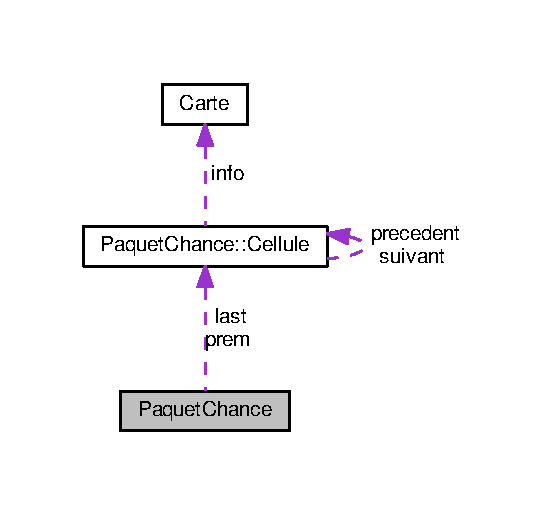
\includegraphics[width=261pt]{classPaquetChance__coll__graph}
\end{center}
\end{figure}
\subsection*{Classes}
\begin{DoxyCompactItemize}
\item 
struct \hyperlink{structPaquetChance_1_1Cellule}{Cellule}
\end{DoxyCompactItemize}
\subsection*{Fonctions membres publiques}
\begin{DoxyCompactItemize}
\item 
\hyperlink{classPaquetChance_a10e2c02b35ae31b7a219b18aa58738af}{Paquet\+Chance} ()
\begin{DoxyCompactList}\small\item\em constructeur par defaut de \hyperlink{classPaquetChance}{Paquet\+Chance} \end{DoxyCompactList}\item 
\hyperlink{classPaquetChance_a70a33d05a371aaa92c9c863f7295cb6c}{$\sim$\+Paquet\+Chance} ()
\begin{DoxyCompactList}\small\item\em destructeur de \hyperlink{classPaquetChance}{Paquet\+Chance} \end{DoxyCompactList}\item 
\hyperlink{classPaquetChance}{Paquet\+Chance} \& \hyperlink{classPaquetChance_aed5ae2e16c0deed0229f8716d77757d5}{operator=} (const \hyperlink{classPaquetChance}{Paquet\+Chance} \&p)
\begin{DoxyCompactList}\small\item\em surcharge de l\textquotesingle{}operateur \char`\"{}=\char`\"{} entre deux paquets de \char`\"{}cartes chance\char`\"{} \end{DoxyCompactList}\item 
void \hyperlink{classPaquetChance_a59f3f6915d1acb57be699275dbb4bd4a}{vider} ()
\begin{DoxyCompactList}\small\item\em vide la liste \hyperlink{classPaquetChance}{Paquet\+Chance} de toutes ses cellules (cartes) \end{DoxyCompactList}\item 
bool \hyperlink{classPaquetChance_a0acfade153190db7e0e78494bb5153cb}{est\+Vide} () const 
\begin{DoxyCompactList}\small\item\em verifie si une file est bien vide (true) ou non (false) \end{DoxyCompactList}\item 
unsigned int \hyperlink{classPaquetChance_aa28685cae7faba322a0feb2cdd5042cd}{nb\+Elements} () const 
\begin{DoxyCompactList}\small\item\em Compte le nombre d\textquotesingle{}elements dans la file. \end{DoxyCompactList}\item 
\hyperlink{classCarte}{Carte} $\ast$ \hyperlink{classPaquetChance_a62c4da96b6b93031f38c3c5a4cd78135}{ieme\+Element} (unsigned int indice) const 
\begin{DoxyCompactList}\small\item\em Selectionne la i-\/eme carte de la file. \end{DoxyCompactList}\item 
void \hyperlink{classPaquetChance_a1c7104a9ff1259cc2a45fdc0b7134819}{modifier\+Ieme\+Element} (unsigned int indice, \hyperlink{classCarte}{Carte} $\ast$e)
\begin{DoxyCompactList}\small\item\em Remplace le i-\/eme element par une carte passee en parametre. \end{DoxyCompactList}\item 
void \hyperlink{classPaquetChance_ab46d1935463a61fc90fc0ae804aace0e}{ajouter\+En\+Tete} (\hyperlink{classCarte}{Carte} $\ast$e)
\begin{DoxyCompactList}\small\item\em Ajoute un element passe en parametre au debut de la file. \end{DoxyCompactList}\item 
void \hyperlink{classPaquetChance_ad4dc4397949178b400a6a3d900901876}{ajouter\+En\+Queue} (\hyperlink{classCarte}{Carte} $\ast$e)
\begin{DoxyCompactList}\small\item\em Ajoute un element passe en parametre a la fin de la file. \end{DoxyCompactList}\item 
void \hyperlink{classPaquetChance_a84fe7a3d65941d9a4b2bb5c11a921447}{supprimer\+Tete} ()
\begin{DoxyCompactList}\small\item\em Supprime le premier element de la file. \end{DoxyCompactList}\item 
void \hyperlink{classPaquetChance_a54a91cae366f6d9d42ca2ab577e4be6c}{inserer\+Element} (\hyperlink{classCarte}{Carte} $\ast$e, unsigned int indice)
\begin{DoxyCompactList}\small\item\em Insere une carte a la i-\/eme place de la file. \end{DoxyCompactList}\item 
void \hyperlink{classPaquetChance_ad40f530029945fe7be21c780af927c12}{trier} ()
\begin{DoxyCompactList}\small\item\em Trie la file en fonction de l\textquotesingle{}id des cartes. \end{DoxyCompactList}\item 
\hyperlink{classCarte}{Carte} $\ast$ \hyperlink{classPaquetChance_ab7c14484bb86c08e665391588f477b59}{Piocher\+Carte} ()
\begin{DoxyCompactList}\small\item\em Pioche une carte, execute son effet, et la remet a la fin du paquet. \end{DoxyCompactList}\end{DoxyCompactItemize}
\subsection*{Attributs publics}
\begin{DoxyCompactItemize}
\item 
\hyperlink{structPaquetChance_1_1Cellule}{Cellule} $\ast$ {\bfseries prem}\hypertarget{classPaquetChance_af9be170835453e4b87b99fa7fc464be2}{}\label{classPaquetChance_af9be170835453e4b87b99fa7fc464be2}

\item 
\hyperlink{structPaquetChance_1_1Cellule}{Cellule} $\ast$ {\bfseries last}\hypertarget{classPaquetChance_a839b9ba922cacea202c635a265746b66}{}\label{classPaquetChance_a839b9ba922cacea202c635a265746b66}

\end{DoxyCompactItemize}


\subsection{Description détaillée}
la classe qui permet de generer une case 

\subsection{Documentation des constructeurs et destructeur}
\index{Paquet\+Chance@{Paquet\+Chance}!Paquet\+Chance@{Paquet\+Chance}}
\index{Paquet\+Chance@{Paquet\+Chance}!Paquet\+Chance@{Paquet\+Chance}}
\subsubsection[{\texorpdfstring{Paquet\+Chance()}{PaquetChance()}}]{\setlength{\rightskip}{0pt plus 5cm}Paquet\+Chance\+::\+Paquet\+Chance (
\begin{DoxyParamCaption}
{}
\end{DoxyParamCaption}
)}\hypertarget{classPaquetChance_a10e2c02b35ae31b7a219b18aa58738af}{}\label{classPaquetChance_a10e2c02b35ae31b7a219b18aa58738af}


constructeur par defaut de \hyperlink{classPaquetChance}{Paquet\+Chance} 


\begin{DoxyParams}{Paramètres}
{\em pas} & d\textquotesingle{}argument \\
\hline
\end{DoxyParams}
\begin{DoxyReturn}{Renvoie}
retourne une file de cartes \char`\"{}caisse de communaute\char`\"{} 
\end{DoxyReturn}
\index{Paquet\+Chance@{Paquet\+Chance}!````~Paquet\+Chance@{$\sim$\+Paquet\+Chance}}
\index{````~Paquet\+Chance@{$\sim$\+Paquet\+Chance}!Paquet\+Chance@{Paquet\+Chance}}
\subsubsection[{\texorpdfstring{$\sim$\+Paquet\+Chance()}{~PaquetChance()}}]{\setlength{\rightskip}{0pt plus 5cm}Paquet\+Chance\+::$\sim$\+Paquet\+Chance (
\begin{DoxyParamCaption}
{}
\end{DoxyParamCaption}
)}\hypertarget{classPaquetChance_a70a33d05a371aaa92c9c863f7295cb6c}{}\label{classPaquetChance_a70a33d05a371aaa92c9c863f7295cb6c}


destructeur de \hyperlink{classPaquetChance}{Paquet\+Chance} 


\begin{DoxyParams}{Paramètres}
{\em pas} & d\textquotesingle{}argument \\
\hline
\end{DoxyParams}
\begin{DoxyReturn}{Renvoie}
pas de valeur retournee 
\end{DoxyReturn}


\subsection{Documentation des fonctions membres}
\index{Paquet\+Chance@{Paquet\+Chance}!ajouter\+En\+Queue@{ajouter\+En\+Queue}}
\index{ajouter\+En\+Queue@{ajouter\+En\+Queue}!Paquet\+Chance@{Paquet\+Chance}}
\subsubsection[{\texorpdfstring{ajouter\+En\+Queue(\+Carte $\ast$e)}{ajouterEnQueue(Carte *e)}}]{\setlength{\rightskip}{0pt plus 5cm}void Paquet\+Chance\+::ajouter\+En\+Queue (
\begin{DoxyParamCaption}
\item[{{\bf Carte} $\ast$}]{e}
\end{DoxyParamCaption}
)}\hypertarget{classPaquetChance_ad4dc4397949178b400a6a3d900901876}{}\label{classPaquetChance_ad4dc4397949178b400a6a3d900901876}


Ajoute un element passe en parametre a la fin de la file. 


\begin{DoxyParams}{Paramètres}
{\em $\ast$e} & \hyperlink{classCarte}{Carte} \\
\hline
\end{DoxyParams}
\begin{DoxyReturn}{Renvoie}
pas de valeur retournee 
\end{DoxyReturn}
\index{Paquet\+Chance@{Paquet\+Chance}!ajouter\+En\+Tete@{ajouter\+En\+Tete}}
\index{ajouter\+En\+Tete@{ajouter\+En\+Tete}!Paquet\+Chance@{Paquet\+Chance}}
\subsubsection[{\texorpdfstring{ajouter\+En\+Tete(\+Carte $\ast$e)}{ajouterEnTete(Carte *e)}}]{\setlength{\rightskip}{0pt plus 5cm}void Paquet\+Chance\+::ajouter\+En\+Tete (
\begin{DoxyParamCaption}
\item[{{\bf Carte} $\ast$}]{e}
\end{DoxyParamCaption}
)}\hypertarget{classPaquetChance_ab46d1935463a61fc90fc0ae804aace0e}{}\label{classPaquetChance_ab46d1935463a61fc90fc0ae804aace0e}


Ajoute un element passe en parametre au debut de la file. 


\begin{DoxyParams}{Paramètres}
{\em $\ast$e} & \hyperlink{classCarte}{Carte} \\
\hline
\end{DoxyParams}
\begin{DoxyReturn}{Renvoie}
pas de valeur retournee 
\end{DoxyReturn}
\index{Paquet\+Chance@{Paquet\+Chance}!est\+Vide@{est\+Vide}}
\index{est\+Vide@{est\+Vide}!Paquet\+Chance@{Paquet\+Chance}}
\subsubsection[{\texorpdfstring{est\+Vide() const }{estVide() const }}]{\setlength{\rightskip}{0pt plus 5cm}bool Paquet\+Chance\+::est\+Vide (
\begin{DoxyParamCaption}
{}
\end{DoxyParamCaption}
) const}\hypertarget{classPaquetChance_a0acfade153190db7e0e78494bb5153cb}{}\label{classPaquetChance_a0acfade153190db7e0e78494bb5153cb}


verifie si une file est bien vide (true) ou non (false) 


\begin{DoxyParams}{Paramètres}
{\em pas} & d\textquotesingle{}argument \\
\hline
\end{DoxyParams}
\begin{DoxyReturn}{Renvoie}
retourne un booleen 
\end{DoxyReturn}
\index{Paquet\+Chance@{Paquet\+Chance}!ieme\+Element@{ieme\+Element}}
\index{ieme\+Element@{ieme\+Element}!Paquet\+Chance@{Paquet\+Chance}}
\subsubsection[{\texorpdfstring{ieme\+Element(unsigned int indice) const }{iemeElement(unsigned int indice) const }}]{\setlength{\rightskip}{0pt plus 5cm}{\bf Carte} $\ast$ Paquet\+Chance\+::ieme\+Element (
\begin{DoxyParamCaption}
\item[{unsigned int}]{i}
\end{DoxyParamCaption}
) const}\hypertarget{classPaquetChance_a62c4da96b6b93031f38c3c5a4cd78135}{}\label{classPaquetChance_a62c4da96b6b93031f38c3c5a4cd78135}


Selectionne la i-\/eme carte de la file. 


\begin{DoxyParams}{Paramètres}
{\em indice} & entier positif \\
\hline
\end{DoxyParams}
\begin{DoxyReturn}{Renvoie}
retourne une \hyperlink{classCarte}{Carte} 
\end{DoxyReturn}
\index{Paquet\+Chance@{Paquet\+Chance}!inserer\+Element@{inserer\+Element}}
\index{inserer\+Element@{inserer\+Element}!Paquet\+Chance@{Paquet\+Chance}}
\subsubsection[{\texorpdfstring{inserer\+Element(\+Carte $\ast$e, unsigned int indice)}{insererElement(Carte *e, unsigned int indice)}}]{\setlength{\rightskip}{0pt plus 5cm}void Paquet\+Chance\+::inserer\+Element (
\begin{DoxyParamCaption}
\item[{{\bf Carte} $\ast$}]{e, }
\item[{unsigned int}]{position}
\end{DoxyParamCaption}
)}\hypertarget{classPaquetChance_a54a91cae366f6d9d42ca2ab577e4be6c}{}\label{classPaquetChance_a54a91cae366f6d9d42ca2ab577e4be6c}


Insere une carte a la i-\/eme place de la file. 


\begin{DoxyParams}{Paramètres}
{\em $\ast$e} & \hyperlink{classCarte}{Carte}, indice\+: entier positif \\
\hline
\end{DoxyParams}
\begin{DoxyReturn}{Renvoie}
pas de valeur retournee 
\end{DoxyReturn}
\index{Paquet\+Chance@{Paquet\+Chance}!modifier\+Ieme\+Element@{modifier\+Ieme\+Element}}
\index{modifier\+Ieme\+Element@{modifier\+Ieme\+Element}!Paquet\+Chance@{Paquet\+Chance}}
\subsubsection[{\texorpdfstring{modifier\+Ieme\+Element(unsigned int indice, Carte $\ast$e)}{modifierIemeElement(unsigned int indice, Carte *e)}}]{\setlength{\rightskip}{0pt plus 5cm}void Paquet\+Chance\+::modifier\+Ieme\+Element (
\begin{DoxyParamCaption}
\item[{unsigned int}]{i, }
\item[{{\bf Carte} $\ast$}]{e}
\end{DoxyParamCaption}
)}\hypertarget{classPaquetChance_a1c7104a9ff1259cc2a45fdc0b7134819}{}\label{classPaquetChance_a1c7104a9ff1259cc2a45fdc0b7134819}


Remplace le i-\/eme element par une carte passee en parametre. 


\begin{DoxyParams}{Paramètres}
{\em indice} & entier positif, $\ast$e\+: \hyperlink{classCarte}{Carte} \\
\hline
\end{DoxyParams}
\begin{DoxyReturn}{Renvoie}
pas de valeur retournee 
\end{DoxyReturn}
\index{Paquet\+Chance@{Paquet\+Chance}!nb\+Elements@{nb\+Elements}}
\index{nb\+Elements@{nb\+Elements}!Paquet\+Chance@{Paquet\+Chance}}
\subsubsection[{\texorpdfstring{nb\+Elements() const }{nbElements() const }}]{\setlength{\rightskip}{0pt plus 5cm}unsigned int Paquet\+Chance\+::nb\+Elements (
\begin{DoxyParamCaption}
{}
\end{DoxyParamCaption}
) const}\hypertarget{classPaquetChance_aa28685cae7faba322a0feb2cdd5042cd}{}\label{classPaquetChance_aa28685cae7faba322a0feb2cdd5042cd}


Compte le nombre d\textquotesingle{}elements dans la file. 


\begin{DoxyParams}{Paramètres}
{\em pas} & d\textquotesingle{}argument \\
\hline
\end{DoxyParams}
\begin{DoxyReturn}{Renvoie}
retourne un entier positif 
\end{DoxyReturn}
\index{Paquet\+Chance@{Paquet\+Chance}!operator=@{operator=}}
\index{operator=@{operator=}!Paquet\+Chance@{Paquet\+Chance}}
\subsubsection[{\texorpdfstring{operator=(const Paquet\+Chance \&p)}{operator=(const PaquetChance &p)}}]{\setlength{\rightskip}{0pt plus 5cm}{\bf Paquet\+Chance} \& Paquet\+Chance\+::operator= (
\begin{DoxyParamCaption}
\item[{const {\bf Paquet\+Chance} \&}]{l}
\end{DoxyParamCaption}
)}\hypertarget{classPaquetChance_aed5ae2e16c0deed0229f8716d77757d5}{}\label{classPaquetChance_aed5ae2e16c0deed0229f8716d77757d5}


surcharge de l\textquotesingle{}operateur \char`\"{}=\char`\"{} entre deux paquets de \char`\"{}cartes chance\char`\"{} 


\begin{DoxyParams}{Paramètres}
{\em p} & \hyperlink{classPaquetCaisseComm}{Paquet\+Caisse\+Comm} \\
\hline
\end{DoxyParams}
\begin{DoxyReturn}{Renvoie}
retourne un paquet de \char`\"{}caisse communaute\char`\"{} 
\end{DoxyReturn}
\index{Paquet\+Chance@{Paquet\+Chance}!Piocher\+Carte@{Piocher\+Carte}}
\index{Piocher\+Carte@{Piocher\+Carte}!Paquet\+Chance@{Paquet\+Chance}}
\subsubsection[{\texorpdfstring{Piocher\+Carte()}{PiocherCarte()}}]{\setlength{\rightskip}{0pt plus 5cm}{\bf Carte} $\ast$ Paquet\+Chance\+::\+Piocher\+Carte (
\begin{DoxyParamCaption}
{}
\end{DoxyParamCaption}
)}\hypertarget{classPaquetChance_ab7c14484bb86c08e665391588f477b59}{}\label{classPaquetChance_ab7c14484bb86c08e665391588f477b59}


Pioche une carte, execute son effet, et la remet a la fin du paquet. 


\begin{DoxyParams}{Paramètres}
{\em pas} & d\textquotesingle{}argument \\
\hline
\end{DoxyParams}
\begin{DoxyReturn}{Renvoie}
renvoie une \hyperlink{classCarte}{Carte} 
\end{DoxyReturn}
\index{Paquet\+Chance@{Paquet\+Chance}!supprimer\+Tete@{supprimer\+Tete}}
\index{supprimer\+Tete@{supprimer\+Tete}!Paquet\+Chance@{Paquet\+Chance}}
\subsubsection[{\texorpdfstring{supprimer\+Tete()}{supprimerTete()}}]{\setlength{\rightskip}{0pt plus 5cm}void Paquet\+Chance\+::supprimer\+Tete (
\begin{DoxyParamCaption}
{}
\end{DoxyParamCaption}
)}\hypertarget{classPaquetChance_a84fe7a3d65941d9a4b2bb5c11a921447}{}\label{classPaquetChance_a84fe7a3d65941d9a4b2bb5c11a921447}


Supprime le premier element de la file. 


\begin{DoxyParams}{Paramètres}
{\em pas} & d\textquotesingle{}argument \\
\hline
\end{DoxyParams}
\begin{DoxyReturn}{Renvoie}
pas de valeur retournee 
\end{DoxyReturn}
\index{Paquet\+Chance@{Paquet\+Chance}!trier@{trier}}
\index{trier@{trier}!Paquet\+Chance@{Paquet\+Chance}}
\subsubsection[{\texorpdfstring{trier()}{trier()}}]{\setlength{\rightskip}{0pt plus 5cm}void Paquet\+Chance\+::trier (
\begin{DoxyParamCaption}
{}
\end{DoxyParamCaption}
)}\hypertarget{classPaquetChance_ad40f530029945fe7be21c780af927c12}{}\label{classPaquetChance_ad40f530029945fe7be21c780af927c12}


Trie la file en fonction de l\textquotesingle{}id des cartes. 


\begin{DoxyParams}{Paramètres}
{\em pas} & d\textquotesingle{}argument \\
\hline
\end{DoxyParams}
\begin{DoxyReturn}{Renvoie}
pas de valeur retournee 
\end{DoxyReturn}
\index{Paquet\+Chance@{Paquet\+Chance}!vider@{vider}}
\index{vider@{vider}!Paquet\+Chance@{Paquet\+Chance}}
\subsubsection[{\texorpdfstring{vider()}{vider()}}]{\setlength{\rightskip}{0pt plus 5cm}void Paquet\+Chance\+::vider (
\begin{DoxyParamCaption}
{}
\end{DoxyParamCaption}
)}\hypertarget{classPaquetChance_a59f3f6915d1acb57be699275dbb4bd4a}{}\label{classPaquetChance_a59f3f6915d1acb57be699275dbb4bd4a}


vide la liste \hyperlink{classPaquetChance}{Paquet\+Chance} de toutes ses cellules (cartes) 


\begin{DoxyParams}{Paramètres}
{\em pas} & d\textquotesingle{}argument \\
\hline
\end{DoxyParams}
\begin{DoxyReturn}{Renvoie}
pas de valeur retournee 
\end{DoxyReturn}


La documentation de cette classe a été générée à partir des fichiers suivants \+:\begin{DoxyCompactItemize}
\item 
src/txt/\hyperlink{PaquetChance_8h}{Paquet\+Chance.\+h}\item 
src/txt/\hyperlink{PaquetChance_8cpp}{Paquet\+Chance.\+cpp}\end{DoxyCompactItemize}

\hypertarget{classPlateau}{}\section{Référence de la classe Plateau}
\label{classPlateau}\index{Plateau@{Plateau}}


{\ttfamily \#include $<$Plateau.\+h$>$}



Graphe de collaboration de Plateau\+:
\nopagebreak
\begin{figure}[H]
\begin{center}
\leavevmode
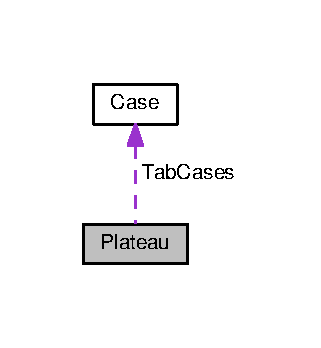
\includegraphics[width=154pt]{classPlateau__coll__graph}
\end{center}
\end{figure}
\subsection*{Fonctions membres publiques}
\begin{DoxyCompactItemize}
\item 
\hyperlink{classPlateau_a07026170529dd928238ee45de0a797d7}{Plateau} ()
\begin{DoxyCompactList}\small\item\em Constructeur par defaut de \hyperlink{classPlateau}{Plateau}. \end{DoxyCompactList}\item 
\hyperlink{classPlateau_a0e6ae72e4d7e9923f996c1247e6a6c8b}{$\sim$\+Plateau} ()
\begin{DoxyCompactList}\small\item\em Destructeur de \hyperlink{classPlateau}{Plateau}. \end{DoxyCompactList}\item 
\hyperlink{classCase}{Case} \hyperlink{classPlateau_a89c2b3450489c02dee04dfeaad576ddd}{get\+Tab\+Cases} (int x) const 
\begin{DoxyCompactList}\small\item\em Cherche la i-\/eme case du tableau de cases. \end{DoxyCompactList}\end{DoxyCompactItemize}
\subsection*{Attributs publics}
\begin{DoxyCompactItemize}
\item 
\hyperlink{classCase}{Case} $\ast$ {\bfseries Tab\+Cases}\hypertarget{classPlateau_a11cb9a16b9e7f696357a4cceac29ca89}{}\label{classPlateau_a11cb9a16b9e7f696357a4cceac29ca89}

\end{DoxyCompactItemize}


\subsection{Description détaillée}
la classe qui permet de generer une case 

\subsection{Documentation des constructeurs et destructeur}
\index{Plateau@{Plateau}!Plateau@{Plateau}}
\index{Plateau@{Plateau}!Plateau@{Plateau}}
\subsubsection[{\texorpdfstring{Plateau()}{Plateau()}}]{\setlength{\rightskip}{0pt plus 5cm}Plateau\+::\+Plateau (
\begin{DoxyParamCaption}
{}
\end{DoxyParamCaption}
)}\hypertarget{classPlateau_a07026170529dd928238ee45de0a797d7}{}\label{classPlateau_a07026170529dd928238ee45de0a797d7}


Constructeur par defaut de \hyperlink{classPlateau}{Plateau}. 


\begin{DoxyParams}{Paramètres}
{\em pas} & d\textquotesingle{}argument \\
\hline
\end{DoxyParams}
\begin{DoxyReturn}{Renvoie}
renvoie un \hyperlink{classPlateau}{Plateau} 
\end{DoxyReturn}
\index{Plateau@{Plateau}!````~Plateau@{$\sim$\+Plateau}}
\index{````~Plateau@{$\sim$\+Plateau}!Plateau@{Plateau}}
\subsubsection[{\texorpdfstring{$\sim$\+Plateau()}{~Plateau()}}]{\setlength{\rightskip}{0pt plus 5cm}Plateau\+::$\sim$\+Plateau (
\begin{DoxyParamCaption}
{}
\end{DoxyParamCaption}
)}\hypertarget{classPlateau_a0e6ae72e4d7e9923f996c1247e6a6c8b}{}\label{classPlateau_a0e6ae72e4d7e9923f996c1247e6a6c8b}


Destructeur de \hyperlink{classPlateau}{Plateau}. 


\begin{DoxyParams}{Paramètres}
{\em pas} & d\textquotesingle{}argument \\
\hline
\end{DoxyParams}
\begin{DoxyReturn}{Renvoie}
pas de valeur retournee 
\end{DoxyReturn}


\subsection{Documentation des fonctions membres}
\index{Plateau@{Plateau}!get\+Tab\+Cases@{get\+Tab\+Cases}}
\index{get\+Tab\+Cases@{get\+Tab\+Cases}!Plateau@{Plateau}}
\subsubsection[{\texorpdfstring{get\+Tab\+Cases(int x) const }{getTabCases(int x) const }}]{\setlength{\rightskip}{0pt plus 5cm}{\bf Case} Plateau\+::get\+Tab\+Cases (
\begin{DoxyParamCaption}
\item[{int}]{x}
\end{DoxyParamCaption}
) const}\hypertarget{classPlateau_a89c2b3450489c02dee04dfeaad576ddd}{}\label{classPlateau_a89c2b3450489c02dee04dfeaad576ddd}


Cherche la i-\/eme case du tableau de cases. 


\begin{DoxyParams}{Paramètres}
{\em x} & entier \\
\hline
\end{DoxyParams}
\begin{DoxyReturn}{Renvoie}
renvoie une \hyperlink{classCase}{Case} 
\end{DoxyReturn}


La documentation de cette classe a été générée à partir des fichiers suivants \+:\begin{DoxyCompactItemize}
\item 
src/txt/\hyperlink{Plateau_8h}{Plateau.\+h}\item 
src/txt/\hyperlink{Plateau_8cpp}{Plateau.\+cpp}\end{DoxyCompactItemize}

\hypertarget{classPropriete}{}\section{Référence de la classe Propriete}
\label{classPropriete}\index{Propriete@{Propriete}}


{\ttfamily \#include $<$Propriete.\+h$>$}

\subsection*{Fonctions membres publiques}
\begin{DoxyCompactItemize}
\item 
\hyperlink{classPropriete_a0ad3dee14b2e7c5c6b0f5e3f9bd6fb69}{Propriete} ()
\begin{DoxyCompactList}\small\item\em Constructeur par defaut de \hyperlink{classPropriete}{Propriete}. \end{DoxyCompactList}\item 
\hyperlink{classPropriete_a8a8eba0f92fcc745ca4caf3868a910c1}{Propriete} (string Nom, int Prix\+Terrain\+Nu, int Prix\+Maison, int Val\+Hypotheque, int $\ast$Taxes\+Propriete, int Proprietaire, int Nb\+Maisons, \hyperlink{classCouleur}{Couleur} couleur, bool Hypotheque, int Nb\+Famille)
\begin{DoxyCompactList}\small\item\em Constructeur par parametre de \hyperlink{classPlateau}{Plateau}. \end{DoxyCompactList}\item 
\hyperlink{classPropriete}{Propriete} $\ast$ \hyperlink{classPropriete_a3ba09ae6e32e9010ecc1742e2a0d998a}{operator=} (\hyperlink{classPropriete}{Propriete} $\ast$propriete\+Droite)
\begin{DoxyCompactList}\small\item\em Surcharge de l\textquotesingle{}operateur \char`\"{}=\char`\"{} entre deux \hyperlink{classPropriete}{Propriete}. \end{DoxyCompactList}\item 
bool \hyperlink{classPropriete_a9e0f646038795f211129a3005079523b}{operator==} (\hyperlink{classPropriete}{Propriete} propriete\+Droite)
\begin{DoxyCompactList}\small\item\em Surcharge de l\textquotesingle{}operateur \char`\"{}==\char`\"{} entre deux \hyperlink{classPropriete}{Propriete}. \end{DoxyCompactList}\item 
string \hyperlink{classPropriete_ac2f237f87a384e2c1227b471bbda889c}{get\+Nom} () const 
\begin{DoxyCompactList}\small\item\em obtenir le nom d\textquotesingle{}une propriete \end{DoxyCompactList}\item 
int \hyperlink{classPropriete_a3171ba14fb6df11e6f4cdee179e0311e}{get\+Prix\+Terrain\+Nu} () const 
\begin{DoxyCompactList}\small\item\em obtenir le prix d\textquotesingle{}un terrain nu (sans maison) \end{DoxyCompactList}\item 
int \hyperlink{classPropriete_a0349bbabae125e3ae1868b30a9d83628}{get\+Prix\+Maison} () const 
\begin{DoxyCompactList}\small\item\em obtenir le prix d\textquotesingle{}une maison \end{DoxyCompactList}\item 
int \hyperlink{classPropriete_a818ce7499d6e34c8cba413f4c7fc1980}{get\+Val\+Hypotheque} () const 
\begin{DoxyCompactList}\small\item\em obtenir la valeur de l\textquotesingle{}hypotheque d\textquotesingle{}une maison \end{DoxyCompactList}\item 
int \hyperlink{classPropriete_a3122317d919b87da44ec240aed7dff62}{get\+Taxes\+Propriete} (int i) const 
\begin{DoxyCompactList}\small\item\em obtenir le rang de la taxe d\textquotesingle{}une \hyperlink{classPropriete}{Propriete} \end{DoxyCompactList}\item 
int \hyperlink{classPropriete_a006c7b50d9d7d7da46ba76e43825595e}{get\+Proprietaire} () const 
\begin{DoxyCompactList}\small\item\em Trouver le proprietaire d\textquotesingle{}une \hyperlink{classPropriete}{Propriete}. \end{DoxyCompactList}\item 
int \hyperlink{classPropriete_ac69da1f6e060e536b7f6f0aaee73e1b2}{get\+Nb\+Maisons} () const 
\begin{DoxyCompactList}\small\item\em obtenir le nombre de maison sur une propriete \end{DoxyCompactList}\item 
\hyperlink{classCouleur}{Couleur} \hyperlink{classPropriete_ac0a961266a4a34726fc09706f7ada70c}{get\+Couleur} () const 
\begin{DoxyCompactList}\small\item\em obtenir la couleur d\textquotesingle{}une propriete \end{DoxyCompactList}\item 
bool \hyperlink{classPropriete_ad4c76cf1b1e1e5081b10445f3b2eb3bc}{get\+Hypotheque} () const 
\begin{DoxyCompactList}\small\item\em obtenir le montant de l\textquotesingle{}hypotheque d\textquotesingle{}une \hyperlink{classPropriete}{Propriete} \end{DoxyCompactList}\item 
void \hyperlink{classPropriete_aaa4cb797b5ca4068c3e1154407726566}{set\+Nom} (string nomprop)
\begin{DoxyCompactList}\small\item\em modifier le nom d\textquotesingle{}une \hyperlink{classPropriete}{Propriete} \end{DoxyCompactList}\item 
void \hyperlink{classPropriete_a513be0d07d243282d5f33d72ee478356}{set\+Prix\+Terrain\+Nu} (int x)
\begin{DoxyCompactList}\small\item\em modifier le prix d\textquotesingle{}un terrain nu \end{DoxyCompactList}\item 
void \hyperlink{classPropriete_a43b101d4b05db64c193094dbe0a20d00}{set\+Prix\+Maison} (int x)
\begin{DoxyCompactList}\small\item\em modifier le prix d\textquotesingle{}une maison \end{DoxyCompactList}\item 
void \hyperlink{classPropriete_ab7d23b4a14f650f3540a44fa2c4da922}{set\+Val\+Hypotheque} (int x)
\begin{DoxyCompactList}\small\item\em modifier le prix de la valeur d\textquotesingle{}une hypotheque \end{DoxyCompactList}\item 
void \hyperlink{classPropriete_a4833cafa66f5635ddb8037bc07fe13e2}{set\+Taxes\+Propriete} (int $\ast$tab)
\begin{DoxyCompactList}\small\item\em modifier le tableau qui classe le rang des taxes de la propriete \end{DoxyCompactList}\item 
void \hyperlink{classPropriete_a622ae8f8fbb32d7918d81fa0bc3d8a4e}{set\+Proprietaire} (int j)
\begin{DoxyCompactList}\small\item\em modifier le proprietaire d\textquotesingle{}une \hyperlink{classPropriete}{Propriete} \end{DoxyCompactList}\item 
void \hyperlink{classPropriete_ae947a56ea6c4692e42d0cf8314ccfc62}{set\+Nb\+Maisons} (int x)
\begin{DoxyCompactList}\small\item\em modifier le nombre de maisons d\textquotesingle{}une \hyperlink{classPropriete}{Propriete} \end{DoxyCompactList}\item 
void \hyperlink{classPropriete_a49777433231ed442b660d4af803c01dc}{set\+Couleur} (\hyperlink{classCouleur}{Couleur} c)
\begin{DoxyCompactList}\small\item\em modifier la couleur d\textquotesingle{}une \hyperlink{classPropriete}{Propriete} \end{DoxyCompactList}\item 
void \hyperlink{classPropriete_a68750bee273997b846947afde0021165}{set\+Hypotheque} (bool x)
\begin{DoxyCompactList}\small\item\em modifier la valeur de l\textquotesingle{}hypotheque d\textquotesingle{}une \hyperlink{classPropriete}{Propriete} \end{DoxyCompactList}\item 
void \hyperlink{classPropriete_a265e57e36532f40e69b78566c307e144}{Ajouter\+Maison} (\hyperlink{classJoueur}{Joueur} $\ast$j)
\begin{DoxyCompactList}\small\item\em modifier le prix d\textquotesingle{}une maison \end{DoxyCompactList}\item 
void \hyperlink{classPropriete_aa595e624672da66ea8de9742ab96eccd}{Hypothequer} (\hyperlink{classJoueur}{Joueur} $\ast$j)
\begin{DoxyCompactList}\small\item\em Vend les maisons et place la \hyperlink{classPropriete}{Propriete} en hypotheque. \end{DoxyCompactList}\item 
void \hyperlink{classPropriete_a4fc5e707a9ac2f947dd071198a49960c}{Change\+Proprietaire} (int NouveauP)
\begin{DoxyCompactList}\small\item\em modifier le proprietaire d\textquotesingle{}une \hyperlink{classPropriete}{Propriete} \end{DoxyCompactList}\item 
void \hyperlink{classPropriete_a35edd9b1d8c58376089f1c1cf6139740}{Payer\+Loyer} (\hyperlink{classJoueur}{Joueur} Client)
\begin{DoxyCompactList}\small\item\em Fait payer un joueur non proprietaire lorsqu\textquotesingle{}il passe sur cette \hyperlink{classPropriete}{Propriete}. \end{DoxyCompactList}\item 
void \hyperlink{classPropriete_a0d7831c65ca007d796e5485331195d20}{Vendre\+Maison} (int Nb\+Maison, \hyperlink{classJoueur}{Joueur} $\ast$j)
\begin{DoxyCompactList}\small\item\em Vend un certain nombre de maisons d\textquotesingle{}une \hyperlink{classPropriete}{Propriete}. \end{DoxyCompactList}\end{DoxyCompactItemize}


\subsection{Description détaillée}
la classe qui permet de generer une case 

\subsection{Documentation des constructeurs et destructeur}
\index{Propriete@{Propriete}!Propriete@{Propriete}}
\index{Propriete@{Propriete}!Propriete@{Propriete}}
\subsubsection[{\texorpdfstring{Propriete()}{Propriete()}}]{\setlength{\rightskip}{0pt plus 5cm}Propriete\+::\+Propriete (
\begin{DoxyParamCaption}
{}
\end{DoxyParamCaption}
)}\hypertarget{classPropriete_a0ad3dee14b2e7c5c6b0f5e3f9bd6fb69}{}\label{classPropriete_a0ad3dee14b2e7c5c6b0f5e3f9bd6fb69}


Constructeur par defaut de \hyperlink{classPropriete}{Propriete}. 


\begin{DoxyParams}{Paramètres}
{\em pas} & d\textquotesingle{}argument \\
\hline
\end{DoxyParams}
\begin{DoxyReturn}{Renvoie}
renvoie une \hyperlink{classPropriete}{Propriete} 
\end{DoxyReturn}
\index{Propriete@{Propriete}!Propriete@{Propriete}}
\index{Propriete@{Propriete}!Propriete@{Propriete}}
\subsubsection[{\texorpdfstring{Propriete(string Nom, int Prix\+Terrain\+Nu, int Prix\+Maison, int Val\+Hypotheque, int $\ast$\+Taxes\+Propriete, int Proprietaire, int Nb\+Maisons, Couleur couleur, bool Hypotheque, int Nb\+Famille)}{Propriete(string Nom, int PrixTerrainNu, int PrixMaison, int ValHypotheque, int *TaxesPropriete, int Proprietaire, int NbMaisons, Couleur couleur, bool Hypotheque, int NbFamille)}}]{\setlength{\rightskip}{0pt plus 5cm}Propriete\+::\+Propriete (
\begin{DoxyParamCaption}
\item[{string}]{Nom2, }
\item[{int}]{Prix\+Terrain\+Nu2, }
\item[{int}]{Prix\+Maison2, }
\item[{int}]{Val\+Hypotheque2, }
\item[{int $\ast$}]{Taxes\+Propriete2, }
\item[{int}]{Proprietaire2, }
\item[{int}]{Nb\+Maisons2, }
\item[{{\bf Couleur}}]{couleur2, }
\item[{bool}]{Hypotheque2, }
\item[{int}]{Nb\+Famille2}
\end{DoxyParamCaption}
)}\hypertarget{classPropriete_a8a8eba0f92fcc745ca4caf3868a910c1}{}\label{classPropriete_a8a8eba0f92fcc745ca4caf3868a910c1}


Constructeur par parametre de \hyperlink{classPlateau}{Plateau}. 


\begin{DoxyParams}{Paramètres}
{\em Nom} & chaine de caractere, Prix\+Terrain\+Nu\+: entier, Prix\+Maison\+: entier, Val\+Hypotheque\+: entier, $\ast$\+Taxes\+Propriete\+: entier, Proprietaire\+: entier, Nb\+Maisons\+: entier, couleur\+: \hyperlink{classCouleur}{Couleur}, Hypotheque\+: booleen, Nb\+Famille\+: entier \\
\hline
\end{DoxyParams}
\begin{DoxyReturn}{Renvoie}
renvoie une \hyperlink{classPropriete}{Propriete} 
\end{DoxyReturn}


\subsection{Documentation des fonctions membres}
\index{Propriete@{Propriete}!Ajouter\+Maison@{Ajouter\+Maison}}
\index{Ajouter\+Maison@{Ajouter\+Maison}!Propriete@{Propriete}}
\subsubsection[{\texorpdfstring{Ajouter\+Maison(\+Joueur $\ast$j)}{AjouterMaison(Joueur *j)}}]{\setlength{\rightskip}{0pt plus 5cm}void Propriete\+::\+Ajouter\+Maison (
\begin{DoxyParamCaption}
\item[{{\bf Joueur} $\ast$}]{j}
\end{DoxyParamCaption}
)}\hypertarget{classPropriete_a265e57e36532f40e69b78566c307e144}{}\label{classPropriete_a265e57e36532f40e69b78566c307e144}


modifier le prix d\textquotesingle{}une maison 

Ajoute une maison a la \hyperlink{classPropriete}{Propriete}.


\begin{DoxyParams}{Paramètres}
{\em x\+:entier} & \\
\hline
\end{DoxyParams}
\begin{DoxyReturn}{Renvoie}
pas de valeur retournee Ajoute une maison a la \hyperlink{classPropriete}{Propriete} 
\end{DoxyReturn}

\begin{DoxyParams}{Paramètres}
{\em $\ast$j} & \hyperlink{classJoueur}{Joueur} \\
\hline
\end{DoxyParams}
\begin{DoxyReturn}{Renvoie}
pas de valeur retournee
\end{DoxyReturn}

\begin{DoxyParams}{Paramètres}
{\em $\ast$j} & \hyperlink{classJoueur}{Joueur} \\
\hline
\end{DoxyParams}
\begin{DoxyReturn}{Renvoie}
pas de valeur retournee 
\end{DoxyReturn}
\index{Propriete@{Propriete}!Change\+Proprietaire@{Change\+Proprietaire}}
\index{Change\+Proprietaire@{Change\+Proprietaire}!Propriete@{Propriete}}
\subsubsection[{\texorpdfstring{Change\+Proprietaire(int Nouveau\+P)}{ChangeProprietaire(int NouveauP)}}]{\setlength{\rightskip}{0pt plus 5cm}void Propriete\+::\+Change\+Proprietaire (
\begin{DoxyParamCaption}
\item[{int}]{NouveauP}
\end{DoxyParamCaption}
)}\hypertarget{classPropriete_a4fc5e707a9ac2f947dd071198a49960c}{}\label{classPropriete_a4fc5e707a9ac2f947dd071198a49960c}


modifier le proprietaire d\textquotesingle{}une \hyperlink{classPropriete}{Propriete} 


\begin{DoxyParams}{Paramètres}
{\em NouveauP} & entier \\
\hline
\end{DoxyParams}
\begin{DoxyReturn}{Renvoie}
pas de valeur retournee 
\end{DoxyReturn}
\index{Propriete@{Propriete}!get\+Couleur@{get\+Couleur}}
\index{get\+Couleur@{get\+Couleur}!Propriete@{Propriete}}
\subsubsection[{\texorpdfstring{get\+Couleur() const }{getCouleur() const }}]{\setlength{\rightskip}{0pt plus 5cm}{\bf Couleur} Propriete\+::get\+Couleur (
\begin{DoxyParamCaption}
{}
\end{DoxyParamCaption}
) const}\hypertarget{classPropriete_ac0a961266a4a34726fc09706f7ada70c}{}\label{classPropriete_ac0a961266a4a34726fc09706f7ada70c}


obtenir la couleur d\textquotesingle{}une propriete 


\begin{DoxyParams}{Paramètres}
{\em pas} & d\textquotesingle{}argument \\
\hline
\end{DoxyParams}
\begin{DoxyReturn}{Renvoie}
retourne une \hyperlink{classCouleur}{Couleur} 
\end{DoxyReturn}
\index{Propriete@{Propriete}!get\+Hypotheque@{get\+Hypotheque}}
\index{get\+Hypotheque@{get\+Hypotheque}!Propriete@{Propriete}}
\subsubsection[{\texorpdfstring{get\+Hypotheque() const }{getHypotheque() const }}]{\setlength{\rightskip}{0pt plus 5cm}bool Propriete\+::get\+Hypotheque (
\begin{DoxyParamCaption}
{}
\end{DoxyParamCaption}
) const}\hypertarget{classPropriete_ad4c76cf1b1e1e5081b10445f3b2eb3bc}{}\label{classPropriete_ad4c76cf1b1e1e5081b10445f3b2eb3bc}


obtenir le montant de l\textquotesingle{}hypotheque d\textquotesingle{}une \hyperlink{classPropriete}{Propriete} 


\begin{DoxyParams}{Paramètres}
{\em pas} & d\textquotesingle{}argument \\
\hline
\end{DoxyParams}
\begin{DoxyReturn}{Renvoie}
retourne un booleen 
\end{DoxyReturn}
\index{Propriete@{Propriete}!get\+Nb\+Maisons@{get\+Nb\+Maisons}}
\index{get\+Nb\+Maisons@{get\+Nb\+Maisons}!Propriete@{Propriete}}
\subsubsection[{\texorpdfstring{get\+Nb\+Maisons() const }{getNbMaisons() const }}]{\setlength{\rightskip}{0pt plus 5cm}int Propriete\+::get\+Nb\+Maisons (
\begin{DoxyParamCaption}
{}
\end{DoxyParamCaption}
) const}\hypertarget{classPropriete_ac69da1f6e060e536b7f6f0aaee73e1b2}{}\label{classPropriete_ac69da1f6e060e536b7f6f0aaee73e1b2}


obtenir le nombre de maison sur une propriete 


\begin{DoxyParams}{Paramètres}
{\em pas} & d\textquotesingle{}argument \\
\hline
\end{DoxyParams}
\begin{DoxyReturn}{Renvoie}
retourne un entier 
\end{DoxyReturn}
\index{Propriete@{Propriete}!get\+Nom@{get\+Nom}}
\index{get\+Nom@{get\+Nom}!Propriete@{Propriete}}
\subsubsection[{\texorpdfstring{get\+Nom() const }{getNom() const }}]{\setlength{\rightskip}{0pt plus 5cm}string Propriete\+::get\+Nom (
\begin{DoxyParamCaption}
{}
\end{DoxyParamCaption}
) const}\hypertarget{classPropriete_ac2f237f87a384e2c1227b471bbda889c}{}\label{classPropriete_ac2f237f87a384e2c1227b471bbda889c}


obtenir le nom d\textquotesingle{}une propriete 


\begin{DoxyParams}{Paramètres}
{\em pas} & d\textquotesingle{}argument \\
\hline
\end{DoxyParams}
\begin{DoxyReturn}{Renvoie}
retourne une chaine de caractere 
\end{DoxyReturn}
\index{Propriete@{Propriete}!get\+Prix\+Maison@{get\+Prix\+Maison}}
\index{get\+Prix\+Maison@{get\+Prix\+Maison}!Propriete@{Propriete}}
\subsubsection[{\texorpdfstring{get\+Prix\+Maison() const }{getPrixMaison() const }}]{\setlength{\rightskip}{0pt plus 5cm}int Propriete\+::get\+Prix\+Maison (
\begin{DoxyParamCaption}
{}
\end{DoxyParamCaption}
) const}\hypertarget{classPropriete_a0349bbabae125e3ae1868b30a9d83628}{}\label{classPropriete_a0349bbabae125e3ae1868b30a9d83628}


obtenir le prix d\textquotesingle{}une maison 


\begin{DoxyParams}{Paramètres}
{\em pas} & d\textquotesingle{}argument \\
\hline
\end{DoxyParams}
\begin{DoxyReturn}{Renvoie}
retourne un entier 
\end{DoxyReturn}
\index{Propriete@{Propriete}!get\+Prix\+Terrain\+Nu@{get\+Prix\+Terrain\+Nu}}
\index{get\+Prix\+Terrain\+Nu@{get\+Prix\+Terrain\+Nu}!Propriete@{Propriete}}
\subsubsection[{\texorpdfstring{get\+Prix\+Terrain\+Nu() const }{getPrixTerrainNu() const }}]{\setlength{\rightskip}{0pt plus 5cm}int Propriete\+::get\+Prix\+Terrain\+Nu (
\begin{DoxyParamCaption}
{}
\end{DoxyParamCaption}
) const}\hypertarget{classPropriete_a3171ba14fb6df11e6f4cdee179e0311e}{}\label{classPropriete_a3171ba14fb6df11e6f4cdee179e0311e}


obtenir le prix d\textquotesingle{}un terrain nu (sans maison) 


\begin{DoxyParams}{Paramètres}
{\em pas} & d\textquotesingle{}argument \\
\hline
\end{DoxyParams}
\begin{DoxyReturn}{Renvoie}
retourne un entier 
\end{DoxyReturn}
\index{Propriete@{Propriete}!get\+Proprietaire@{get\+Proprietaire}}
\index{get\+Proprietaire@{get\+Proprietaire}!Propriete@{Propriete}}
\subsubsection[{\texorpdfstring{get\+Proprietaire() const }{getProprietaire() const }}]{\setlength{\rightskip}{0pt plus 5cm}int Propriete\+::get\+Proprietaire (
\begin{DoxyParamCaption}
{}
\end{DoxyParamCaption}
) const}\hypertarget{classPropriete_a006c7b50d9d7d7da46ba76e43825595e}{}\label{classPropriete_a006c7b50d9d7d7da46ba76e43825595e}


Trouver le proprietaire d\textquotesingle{}une \hyperlink{classPropriete}{Propriete}. 


\begin{DoxyParams}{Paramètres}
{\em pas} & d\textquotesingle{}argument \\
\hline
\end{DoxyParams}
\begin{DoxyReturn}{Renvoie}
retourne un entier 
\end{DoxyReturn}
\index{Propriete@{Propriete}!get\+Taxes\+Propriete@{get\+Taxes\+Propriete}}
\index{get\+Taxes\+Propriete@{get\+Taxes\+Propriete}!Propriete@{Propriete}}
\subsubsection[{\texorpdfstring{get\+Taxes\+Propriete(int i) const }{getTaxesPropriete(int i) const }}]{\setlength{\rightskip}{0pt plus 5cm}int Propriete\+::get\+Taxes\+Propriete (
\begin{DoxyParamCaption}
\item[{int}]{i}
\end{DoxyParamCaption}
) const}\hypertarget{classPropriete_a3122317d919b87da44ec240aed7dff62}{}\label{classPropriete_a3122317d919b87da44ec240aed7dff62}


obtenir le rang de la taxe d\textquotesingle{}une \hyperlink{classPropriete}{Propriete} 


\begin{DoxyParams}{Paramètres}
{\em i} & entier \\
\hline
\end{DoxyParams}
\begin{DoxyReturn}{Renvoie}
retourne un entier 
\end{DoxyReturn}
\index{Propriete@{Propriete}!get\+Val\+Hypotheque@{get\+Val\+Hypotheque}}
\index{get\+Val\+Hypotheque@{get\+Val\+Hypotheque}!Propriete@{Propriete}}
\subsubsection[{\texorpdfstring{get\+Val\+Hypotheque() const }{getValHypotheque() const }}]{\setlength{\rightskip}{0pt plus 5cm}int Propriete\+::get\+Val\+Hypotheque (
\begin{DoxyParamCaption}
{}
\end{DoxyParamCaption}
) const}\hypertarget{classPropriete_a818ce7499d6e34c8cba413f4c7fc1980}{}\label{classPropriete_a818ce7499d6e34c8cba413f4c7fc1980}


obtenir la valeur de l\textquotesingle{}hypotheque d\textquotesingle{}une maison 


\begin{DoxyParams}{Paramètres}
{\em pas} & d\textquotesingle{}argument \\
\hline
\end{DoxyParams}
\begin{DoxyReturn}{Renvoie}
retourne un entier 
\end{DoxyReturn}
\index{Propriete@{Propriete}!Hypothequer@{Hypothequer}}
\index{Hypothequer@{Hypothequer}!Propriete@{Propriete}}
\subsubsection[{\texorpdfstring{Hypothequer(\+Joueur $\ast$j)}{Hypothequer(Joueur *j)}}]{\setlength{\rightskip}{0pt plus 5cm}void Propriete\+::\+Hypothequer (
\begin{DoxyParamCaption}
\item[{{\bf Joueur} $\ast$}]{j}
\end{DoxyParamCaption}
)}\hypertarget{classPropriete_aa595e624672da66ea8de9742ab96eccd}{}\label{classPropriete_aa595e624672da66ea8de9742ab96eccd}


Vend les maisons et place la \hyperlink{classPropriete}{Propriete} en hypotheque. 


\begin{DoxyParams}{Paramètres}
{\em $\ast$j} & \hyperlink{classJoueur}{Joueur} \\
\hline
\end{DoxyParams}
\begin{DoxyReturn}{Renvoie}
pas de valeur retournee 
\end{DoxyReturn}
\index{Propriete@{Propriete}!operator=@{operator=}}
\index{operator=@{operator=}!Propriete@{Propriete}}
\subsubsection[{\texorpdfstring{operator=(\+Propriete $\ast$propriete\+Droite)}{operator=(Propriete *proprieteDroite)}}]{\setlength{\rightskip}{0pt plus 5cm}{\bf Propriete} $\ast$ Propriete\+::operator= (
\begin{DoxyParamCaption}
\item[{{\bf Propriete} $\ast$}]{propriete\+Droite}
\end{DoxyParamCaption}
)}\hypertarget{classPropriete_a3ba09ae6e32e9010ecc1742e2a0d998a}{}\label{classPropriete_a3ba09ae6e32e9010ecc1742e2a0d998a}


Surcharge de l\textquotesingle{}operateur \char`\"{}=\char`\"{} entre deux \hyperlink{classPropriete}{Propriete}. 


\begin{DoxyParams}{Paramètres}
{\em $\ast$propriete\+Droite} & \hyperlink{classPropriete}{Propriete} \\
\hline
\end{DoxyParams}
\begin{DoxyReturn}{Renvoie}
renvoie une \hyperlink{classPropriete}{Propriete} 
\end{DoxyReturn}
\index{Propriete@{Propriete}!operator==@{operator==}}
\index{operator==@{operator==}!Propriete@{Propriete}}
\subsubsection[{\texorpdfstring{operator==(\+Propriete propriete\+Droite)}{operator==(Propriete proprieteDroite)}}]{\setlength{\rightskip}{0pt plus 5cm}bool Propriete\+::operator== (
\begin{DoxyParamCaption}
\item[{{\bf Propriete}}]{propriete\+Droite}
\end{DoxyParamCaption}
)}\hypertarget{classPropriete_a9e0f646038795f211129a3005079523b}{}\label{classPropriete_a9e0f646038795f211129a3005079523b}


Surcharge de l\textquotesingle{}operateur \char`\"{}==\char`\"{} entre deux \hyperlink{classPropriete}{Propriete}. 


\begin{DoxyParams}{Paramètres}
{\em propriete\+Droite} & \hyperlink{classPropriete}{Propriete} \\
\hline
\end{DoxyParams}
\begin{DoxyReturn}{Renvoie}
renvoie un booleen 
\end{DoxyReturn}
\index{Propriete@{Propriete}!Payer\+Loyer@{Payer\+Loyer}}
\index{Payer\+Loyer@{Payer\+Loyer}!Propriete@{Propriete}}
\subsubsection[{\texorpdfstring{Payer\+Loyer(\+Joueur Client)}{PayerLoyer(Joueur Client)}}]{\setlength{\rightskip}{0pt plus 5cm}void Propriete\+::\+Payer\+Loyer (
\begin{DoxyParamCaption}
\item[{{\bf Joueur}}]{Client}
\end{DoxyParamCaption}
)}\hypertarget{classPropriete_a35edd9b1d8c58376089f1c1cf6139740}{}\label{classPropriete_a35edd9b1d8c58376089f1c1cf6139740}


Fait payer un joueur non proprietaire lorsqu\textquotesingle{}il passe sur cette \hyperlink{classPropriete}{Propriete}. 


\begin{DoxyParams}{Paramètres}
{\em Client} & \hyperlink{classJoueur}{Joueur} \\
\hline
\end{DoxyParams}
\begin{DoxyReturn}{Renvoie}
pas de valeur retournee 
\end{DoxyReturn}
\index{Propriete@{Propriete}!set\+Couleur@{set\+Couleur}}
\index{set\+Couleur@{set\+Couleur}!Propriete@{Propriete}}
\subsubsection[{\texorpdfstring{set\+Couleur(\+Couleur c)}{setCouleur(Couleur c)}}]{\setlength{\rightskip}{0pt plus 5cm}void Propriete\+::set\+Couleur (
\begin{DoxyParamCaption}
\item[{{\bf Couleur}}]{c}
\end{DoxyParamCaption}
)}\hypertarget{classPropriete_a49777433231ed442b660d4af803c01dc}{}\label{classPropriete_a49777433231ed442b660d4af803c01dc}


modifier la couleur d\textquotesingle{}une \hyperlink{classPropriete}{Propriete} 


\begin{DoxyParams}{Paramètres}
{\em c} & \hyperlink{classCouleur}{Couleur} \\
\hline
\end{DoxyParams}
\begin{DoxyReturn}{Renvoie}
pas de valeur retournee 
\end{DoxyReturn}
\index{Propriete@{Propriete}!set\+Hypotheque@{set\+Hypotheque}}
\index{set\+Hypotheque@{set\+Hypotheque}!Propriete@{Propriete}}
\subsubsection[{\texorpdfstring{set\+Hypotheque(bool x)}{setHypotheque(bool x)}}]{\setlength{\rightskip}{0pt plus 5cm}void Propriete\+::set\+Hypotheque (
\begin{DoxyParamCaption}
\item[{bool}]{x}
\end{DoxyParamCaption}
)}\hypertarget{classPropriete_a68750bee273997b846947afde0021165}{}\label{classPropriete_a68750bee273997b846947afde0021165}


modifier la valeur de l\textquotesingle{}hypotheque d\textquotesingle{}une \hyperlink{classPropriete}{Propriete} 


\begin{DoxyParams}{Paramètres}
{\em x} & booleen \\
\hline
\end{DoxyParams}
\begin{DoxyReturn}{Renvoie}
pas de valeur retournee 
\end{DoxyReturn}
\index{Propriete@{Propriete}!set\+Nb\+Maisons@{set\+Nb\+Maisons}}
\index{set\+Nb\+Maisons@{set\+Nb\+Maisons}!Propriete@{Propriete}}
\subsubsection[{\texorpdfstring{set\+Nb\+Maisons(int x)}{setNbMaisons(int x)}}]{\setlength{\rightskip}{0pt plus 5cm}void Propriete\+::set\+Nb\+Maisons (
\begin{DoxyParamCaption}
\item[{int}]{x}
\end{DoxyParamCaption}
)}\hypertarget{classPropriete_ae947a56ea6c4692e42d0cf8314ccfc62}{}\label{classPropriete_ae947a56ea6c4692e42d0cf8314ccfc62}


modifier le nombre de maisons d\textquotesingle{}une \hyperlink{classPropriete}{Propriete} 


\begin{DoxyParams}{Paramètres}
{\em x} & entier \\
\hline
\end{DoxyParams}
\begin{DoxyReturn}{Renvoie}
pas de valeur retournee 
\end{DoxyReturn}
\index{Propriete@{Propriete}!set\+Nom@{set\+Nom}}
\index{set\+Nom@{set\+Nom}!Propriete@{Propriete}}
\subsubsection[{\texorpdfstring{set\+Nom(string nomprop)}{setNom(string nomprop)}}]{\setlength{\rightskip}{0pt plus 5cm}void Propriete\+::set\+Nom (
\begin{DoxyParamCaption}
\item[{string}]{nomprop}
\end{DoxyParamCaption}
)}\hypertarget{classPropriete_aaa4cb797b5ca4068c3e1154407726566}{}\label{classPropriete_aaa4cb797b5ca4068c3e1154407726566}


modifier le nom d\textquotesingle{}une \hyperlink{classPropriete}{Propriete} 


\begin{DoxyParams}{Paramètres}
{\em nomprop} & chaine de caractere \\
\hline
\end{DoxyParams}
\begin{DoxyReturn}{Renvoie}
pas de valeur retournee 
\end{DoxyReturn}
\index{Propriete@{Propriete}!set\+Prix\+Maison@{set\+Prix\+Maison}}
\index{set\+Prix\+Maison@{set\+Prix\+Maison}!Propriete@{Propriete}}
\subsubsection[{\texorpdfstring{set\+Prix\+Maison(int x)}{setPrixMaison(int x)}}]{\setlength{\rightskip}{0pt plus 5cm}void Propriete\+::set\+Prix\+Maison (
\begin{DoxyParamCaption}
\item[{int}]{x}
\end{DoxyParamCaption}
)}\hypertarget{classPropriete_a43b101d4b05db64c193094dbe0a20d00}{}\label{classPropriete_a43b101d4b05db64c193094dbe0a20d00}


modifier le prix d\textquotesingle{}une maison 


\begin{DoxyParams}{Paramètres}
{\em x} & entier \\
\hline
\end{DoxyParams}
\begin{DoxyReturn}{Renvoie}
pas de valeur retournee 
\end{DoxyReturn}
\index{Propriete@{Propriete}!set\+Prix\+Terrain\+Nu@{set\+Prix\+Terrain\+Nu}}
\index{set\+Prix\+Terrain\+Nu@{set\+Prix\+Terrain\+Nu}!Propriete@{Propriete}}
\subsubsection[{\texorpdfstring{set\+Prix\+Terrain\+Nu(int x)}{setPrixTerrainNu(int x)}}]{\setlength{\rightskip}{0pt plus 5cm}void Propriete\+::set\+Prix\+Terrain\+Nu (
\begin{DoxyParamCaption}
\item[{int}]{x}
\end{DoxyParamCaption}
)}\hypertarget{classPropriete_a513be0d07d243282d5f33d72ee478356}{}\label{classPropriete_a513be0d07d243282d5f33d72ee478356}


modifier le prix d\textquotesingle{}un terrain nu 


\begin{DoxyParams}{Paramètres}
{\em x} & entier \\
\hline
\end{DoxyParams}
\begin{DoxyReturn}{Renvoie}
pas de valeur retournee 
\end{DoxyReturn}
\index{Propriete@{Propriete}!set\+Proprietaire@{set\+Proprietaire}}
\index{set\+Proprietaire@{set\+Proprietaire}!Propriete@{Propriete}}
\subsubsection[{\texorpdfstring{set\+Proprietaire(int j)}{setProprietaire(int j)}}]{\setlength{\rightskip}{0pt plus 5cm}void Propriete\+::set\+Proprietaire (
\begin{DoxyParamCaption}
\item[{int}]{j}
\end{DoxyParamCaption}
)}\hypertarget{classPropriete_a622ae8f8fbb32d7918d81fa0bc3d8a4e}{}\label{classPropriete_a622ae8f8fbb32d7918d81fa0bc3d8a4e}


modifier le proprietaire d\textquotesingle{}une \hyperlink{classPropriete}{Propriete} 


\begin{DoxyParams}{Paramètres}
{\em j} & entier \\
\hline
\end{DoxyParams}
\begin{DoxyReturn}{Renvoie}
pas de valeur retournee 
\end{DoxyReturn}
\index{Propriete@{Propriete}!set\+Taxes\+Propriete@{set\+Taxes\+Propriete}}
\index{set\+Taxes\+Propriete@{set\+Taxes\+Propriete}!Propriete@{Propriete}}
\subsubsection[{\texorpdfstring{set\+Taxes\+Propriete(int $\ast$tab)}{setTaxesPropriete(int *tab)}}]{\setlength{\rightskip}{0pt plus 5cm}void Propriete\+::set\+Taxes\+Propriete (
\begin{DoxyParamCaption}
\item[{int $\ast$}]{tab}
\end{DoxyParamCaption}
)}\hypertarget{classPropriete_a4833cafa66f5635ddb8037bc07fe13e2}{}\label{classPropriete_a4833cafa66f5635ddb8037bc07fe13e2}


modifier le tableau qui classe le rang des taxes de la propriete 


\begin{DoxyParams}{Paramètres}
{\em $\ast$tab} & tableau d\textquotesingle{}entiers \\
\hline
\end{DoxyParams}
\begin{DoxyReturn}{Renvoie}
pas de valeur retournee 
\end{DoxyReturn}
\index{Propriete@{Propriete}!set\+Val\+Hypotheque@{set\+Val\+Hypotheque}}
\index{set\+Val\+Hypotheque@{set\+Val\+Hypotheque}!Propriete@{Propriete}}
\subsubsection[{\texorpdfstring{set\+Val\+Hypotheque(int x)}{setValHypotheque(int x)}}]{\setlength{\rightskip}{0pt plus 5cm}void Propriete\+::set\+Val\+Hypotheque (
\begin{DoxyParamCaption}
\item[{int}]{x}
\end{DoxyParamCaption}
)}\hypertarget{classPropriete_ab7d23b4a14f650f3540a44fa2c4da922}{}\label{classPropriete_ab7d23b4a14f650f3540a44fa2c4da922}


modifier le prix de la valeur d\textquotesingle{}une hypotheque 


\begin{DoxyParams}{Paramètres}
{\em x} & entier \\
\hline
\end{DoxyParams}
\begin{DoxyReturn}{Renvoie}
pas de valeur retournee 
\end{DoxyReturn}
\index{Propriete@{Propriete}!Vendre\+Maison@{Vendre\+Maison}}
\index{Vendre\+Maison@{Vendre\+Maison}!Propriete@{Propriete}}
\subsubsection[{\texorpdfstring{Vendre\+Maison(int Nb\+Maison, Joueur $\ast$j)}{VendreMaison(int NbMaison, Joueur *j)}}]{\setlength{\rightskip}{0pt plus 5cm}void Propriete\+::\+Vendre\+Maison (
\begin{DoxyParamCaption}
\item[{int}]{Nb\+Maison, }
\item[{{\bf Joueur} $\ast$}]{j}
\end{DoxyParamCaption}
)}\hypertarget{classPropriete_a0d7831c65ca007d796e5485331195d20}{}\label{classPropriete_a0d7831c65ca007d796e5485331195d20}


Vend un certain nombre de maisons d\textquotesingle{}une \hyperlink{classPropriete}{Propriete}. 


\begin{DoxyParams}{Paramètres}
{\em Nb\+Maison} & entier, $\ast$j\+: \hyperlink{classJoueur}{Joueur} \\
\hline
\end{DoxyParams}
\begin{DoxyReturn}{Renvoie}
pas de valeur retournee 
\end{DoxyReturn}


La documentation de cette classe a été générée à partir des fichiers suivants \+:\begin{DoxyCompactItemize}
\item 
src/txt/\hyperlink{Propriete_8h}{Propriete.\+h}\item 
src/txt/\hyperlink{Propriete_8cpp}{Propriete.\+cpp}\end{DoxyCompactItemize}

\hypertarget{classsdlJeu}{}\section{Référence de la classe sdl\+Jeu}
\label{classsdlJeu}\index{sdl\+Jeu@{sdl\+Jeu}}


{\ttfamily \#include $<$sdl\+Jeu.\+h$>$}

\subsection*{Fonctions membres publiques}
\begin{DoxyCompactItemize}
\item 
\hyperlink{classsdlJeu_a06ba2075a4b592f6d0a2e268c29a044e}{sdl\+Jeu} ()
\begin{DoxyCompactList}\small\item\em Constructeur par defaut de la classe \hyperlink{classsdlJeu}{sdl\+Jeu} qui initialise l\textquotesingle{}affichage. \end{DoxyCompactList}\item 
\hyperlink{classsdlJeu_a5bcd8f5ed17a2cea2ad2fc633415cbcc}{$\sim$sdl\+Jeu} ()
\begin{DoxyCompactList}\small\item\em Destructeur de la classe \hyperlink{classsdlJeu}{sdl\+Jeu}. \end{DoxyCompactList}\item 
void \hyperlink{classsdlJeu_a5628835d7efcab056985c3aa3de56836}{sdl\+Boucle} ()
\begin{DoxyCompactList}\small\item\em boucle d\textquotesingle{}evenement \end{DoxyCompactList}\item 
void \hyperlink{classsdlJeu_aedada55e3f96ba37493664d358dc7b60}{sdl\+Aff} ()
\begin{DoxyCompactList}\small\item\em affichage de tous les elements de base a l\textquotesingle{}ecran \end{DoxyCompactList}\item 
void {\bfseries sdl\+Init} ()\hypertarget{classsdlJeu_a89c72a786f10e4e794365094fbb70d4f}{}\label{classsdlJeu_a89c72a786f10e4e794365094fbb70d4f}

\item 
void \hyperlink{classsdlJeu_a5d4e5e67c8049b9c603a23e889920ddd}{affiche\+Joueur1} (int argent, int prison, S\+D\+L\+\_\+\+Renderer $\ast$renderer, S\+D\+L\+\_\+\+Color couleur, S\+D\+L\+\_\+\+Color couleurbg)
\begin{DoxyCompactList}\small\item\em affiche les donnees du joueur 1 (argent, carte libere prison) \end{DoxyCompactList}\item 
void \hyperlink{classsdlJeu_abbab72b3546c723725bf58441e44b4d1}{affiche\+Joueur2} (int argent, int prison, S\+D\+L\+\_\+\+Renderer $\ast$renderer, S\+D\+L\+\_\+\+Color couleur, S\+D\+L\+\_\+\+Color couleurbg)
\begin{DoxyCompactList}\small\item\em affiche les donnees du joueur 2 (argent, carte libere prison) \end{DoxyCompactList}\item 
void \hyperlink{classsdlJeu_a8d3ced721c9a382aa41ff58d5ee8b184}{affiche\+Joueur3} (int argent, int prison, S\+D\+L\+\_\+\+Renderer $\ast$renderer, S\+D\+L\+\_\+\+Color couleur, S\+D\+L\+\_\+\+Color couleurbg)
\begin{DoxyCompactList}\small\item\em affiche les donnees du joueur 3 (argent, carte libere prison) \end{DoxyCompactList}\item 
void \hyperlink{classsdlJeu_a517d7dff75b6bd6c4d0feed943dd4897}{affiche\+Joueur4} (int argent, int prison, S\+D\+L\+\_\+\+Renderer $\ast$renderer, S\+D\+L\+\_\+\+Color couleur, S\+D\+L\+\_\+\+Color couleurbg)
\begin{DoxyCompactList}\small\item\em affiche les donnees du joueur 4 (argent, carte libere prison) \end{DoxyCompactList}\item 
void \hyperlink{classsdlJeu_a4f777328ce3e0c2e123d7b0910b179b7}{deplacer\+Joueur} (int numcase, int numJ)
\begin{DoxyCompactList}\small\item\em modifie la position d\textquotesingle{}un joueur \end{DoxyCompactList}\end{DoxyCompactItemize}


\subsection{Description détaillée}
La classe g�rant le jeu avec un affichage S\+DL 

\subsection{Documentation des constructeurs et destructeur}
\index{sdl\+Jeu@{sdl\+Jeu}!sdl\+Jeu@{sdl\+Jeu}}
\index{sdl\+Jeu@{sdl\+Jeu}!sdl\+Jeu@{sdl\+Jeu}}
\subsubsection[{\texorpdfstring{sdl\+Jeu()}{sdlJeu()}}]{\setlength{\rightskip}{0pt plus 5cm}sdl\+Jeu\+::sdl\+Jeu (
\begin{DoxyParamCaption}
{}
\end{DoxyParamCaption}
)}\hypertarget{classsdlJeu_a06ba2075a4b592f6d0a2e268c29a044e}{}\label{classsdlJeu_a06ba2075a4b592f6d0a2e268c29a044e}


Constructeur par defaut de la classe \hyperlink{classsdlJeu}{sdl\+Jeu} qui initialise l\textquotesingle{}affichage. 


\begin{DoxyParams}{Paramètres}
{\em pas} & d\textquotesingle{}argument \\
\hline
\end{DoxyParams}
\begin{DoxyReturn}{Renvoie}
pas de valeur retournee 
\end{DoxyReturn}
\index{sdl\+Jeu@{sdl\+Jeu}!````~sdl\+Jeu@{$\sim$sdl\+Jeu}}
\index{````~sdl\+Jeu@{$\sim$sdl\+Jeu}!sdl\+Jeu@{sdl\+Jeu}}
\subsubsection[{\texorpdfstring{$\sim$sdl\+Jeu()}{~sdlJeu()}}]{\setlength{\rightskip}{0pt plus 5cm}sdl\+Jeu\+::$\sim$sdl\+Jeu (
\begin{DoxyParamCaption}
{}
\end{DoxyParamCaption}
)}\hypertarget{classsdlJeu_a5bcd8f5ed17a2cea2ad2fc633415cbcc}{}\label{classsdlJeu_a5bcd8f5ed17a2cea2ad2fc633415cbcc}


Destructeur de la classe \hyperlink{classsdlJeu}{sdl\+Jeu}. 


\begin{DoxyParams}{Paramètres}
{\em pas} & d\textquotesingle{}argument \\
\hline
\end{DoxyParams}
\begin{DoxyReturn}{Renvoie}
pas de valeur retournee 
\end{DoxyReturn}


\subsection{Documentation des fonctions membres}
\index{sdl\+Jeu@{sdl\+Jeu}!affiche\+Joueur1@{affiche\+Joueur1}}
\index{affiche\+Joueur1@{affiche\+Joueur1}!sdl\+Jeu@{sdl\+Jeu}}
\subsubsection[{\texorpdfstring{affiche\+Joueur1(int argent, int prison, S\+D\+L\+\_\+\+Renderer $\ast$renderer, S\+D\+L\+\_\+\+Color couleur, S\+D\+L\+\_\+\+Color couleurbg)}{afficheJoueur1(int argent, int prison, SDL_Renderer *renderer, SDL_Color couleur, SDL_Color couleurbg)}}]{\setlength{\rightskip}{0pt plus 5cm}void sdl\+Jeu\+::affiche\+Joueur1 (
\begin{DoxyParamCaption}
\item[{int}]{argent, }
\item[{int}]{prison, }
\item[{S\+D\+L\+\_\+\+Renderer $\ast$}]{renderer, }
\item[{S\+D\+L\+\_\+\+Color}]{couleur, }
\item[{S\+D\+L\+\_\+\+Color}]{couleurbg}
\end{DoxyParamCaption}
)}\hypertarget{classsdlJeu_a5d4e5e67c8049b9c603a23e889920ddd}{}\label{classsdlJeu_a5d4e5e67c8049b9c603a23e889920ddd}


affiche les donnees du joueur 1 (argent, carte libere prison) 


\begin{DoxyParams}{Paramètres}
{\em argent} & int,prison\+: int,renderer\+: S\+D\+L\+\_\+\+Renderer $\ast$,couleur\+: S\+D\+L\+\_\+\+Color,couleurbg\+: S\+D\+L\+\_\+\+Color \\
\hline
\end{DoxyParams}
\begin{DoxyReturn}{Renvoie}
pas de valeur retournee 
\end{DoxyReturn}
\index{sdl\+Jeu@{sdl\+Jeu}!affiche\+Joueur2@{affiche\+Joueur2}}
\index{affiche\+Joueur2@{affiche\+Joueur2}!sdl\+Jeu@{sdl\+Jeu}}
\subsubsection[{\texorpdfstring{affiche\+Joueur2(int argent, int prison, S\+D\+L\+\_\+\+Renderer $\ast$renderer, S\+D\+L\+\_\+\+Color couleur, S\+D\+L\+\_\+\+Color couleurbg)}{afficheJoueur2(int argent, int prison, SDL_Renderer *renderer, SDL_Color couleur, SDL_Color couleurbg)}}]{\setlength{\rightskip}{0pt plus 5cm}void sdl\+Jeu\+::affiche\+Joueur2 (
\begin{DoxyParamCaption}
\item[{int}]{argent, }
\item[{int}]{prison, }
\item[{S\+D\+L\+\_\+\+Renderer $\ast$}]{renderer, }
\item[{S\+D\+L\+\_\+\+Color}]{couleur, }
\item[{S\+D\+L\+\_\+\+Color}]{couleurbg}
\end{DoxyParamCaption}
)}\hypertarget{classsdlJeu_abbab72b3546c723725bf58441e44b4d1}{}\label{classsdlJeu_abbab72b3546c723725bf58441e44b4d1}


affiche les donnees du joueur 2 (argent, carte libere prison) 


\begin{DoxyParams}{Paramètres}
{\em argent} & int,prison\+: int,renderer\+: S\+D\+L\+\_\+\+Renderer $\ast$,couleur\+: S\+D\+L\+\_\+\+Color,couleurbg\+: S\+D\+L\+\_\+\+Color \\
\hline
\end{DoxyParams}
\begin{DoxyReturn}{Renvoie}
pas de valeur retournee 
\end{DoxyReturn}
\index{sdl\+Jeu@{sdl\+Jeu}!affiche\+Joueur3@{affiche\+Joueur3}}
\index{affiche\+Joueur3@{affiche\+Joueur3}!sdl\+Jeu@{sdl\+Jeu}}
\subsubsection[{\texorpdfstring{affiche\+Joueur3(int argent, int prison, S\+D\+L\+\_\+\+Renderer $\ast$renderer, S\+D\+L\+\_\+\+Color couleur, S\+D\+L\+\_\+\+Color couleurbg)}{afficheJoueur3(int argent, int prison, SDL_Renderer *renderer, SDL_Color couleur, SDL_Color couleurbg)}}]{\setlength{\rightskip}{0pt plus 5cm}void sdl\+Jeu\+::affiche\+Joueur3 (
\begin{DoxyParamCaption}
\item[{int}]{argent, }
\item[{int}]{prison, }
\item[{S\+D\+L\+\_\+\+Renderer $\ast$}]{renderer, }
\item[{S\+D\+L\+\_\+\+Color}]{couleur, }
\item[{S\+D\+L\+\_\+\+Color}]{couleurbg}
\end{DoxyParamCaption}
)}\hypertarget{classsdlJeu_a8d3ced721c9a382aa41ff58d5ee8b184}{}\label{classsdlJeu_a8d3ced721c9a382aa41ff58d5ee8b184}


affiche les donnees du joueur 3 (argent, carte libere prison) 


\begin{DoxyParams}{Paramètres}
{\em argent} & int,prison\+: int,renderer\+: S\+D\+L\+\_\+\+Renderer $\ast$,couleur\+: S\+D\+L\+\_\+\+Color,couleurbg\+: S\+D\+L\+\_\+\+Color \\
\hline
\end{DoxyParams}
\begin{DoxyReturn}{Renvoie}
pas de valeur retournee 
\end{DoxyReturn}
\index{sdl\+Jeu@{sdl\+Jeu}!affiche\+Joueur4@{affiche\+Joueur4}}
\index{affiche\+Joueur4@{affiche\+Joueur4}!sdl\+Jeu@{sdl\+Jeu}}
\subsubsection[{\texorpdfstring{affiche\+Joueur4(int argent, int prison, S\+D\+L\+\_\+\+Renderer $\ast$renderer, S\+D\+L\+\_\+\+Color couleur, S\+D\+L\+\_\+\+Color couleurbg)}{afficheJoueur4(int argent, int prison, SDL_Renderer *renderer, SDL_Color couleur, SDL_Color couleurbg)}}]{\setlength{\rightskip}{0pt plus 5cm}void sdl\+Jeu\+::affiche\+Joueur4 (
\begin{DoxyParamCaption}
\item[{int}]{argent, }
\item[{int}]{prison, }
\item[{S\+D\+L\+\_\+\+Renderer $\ast$}]{renderer, }
\item[{S\+D\+L\+\_\+\+Color}]{couleur, }
\item[{S\+D\+L\+\_\+\+Color}]{couleurbg}
\end{DoxyParamCaption}
)}\hypertarget{classsdlJeu_a517d7dff75b6bd6c4d0feed943dd4897}{}\label{classsdlJeu_a517d7dff75b6bd6c4d0feed943dd4897}


affiche les donnees du joueur 4 (argent, carte libere prison) 


\begin{DoxyParams}{Paramètres}
{\em argent} & int,prison\+: int,renderer\+: S\+D\+L\+\_\+\+Renderer $\ast$,couleur\+: S\+D\+L\+\_\+\+Color,couleurbg\+: S\+D\+L\+\_\+\+Color \\
\hline
\end{DoxyParams}
\begin{DoxyReturn}{Renvoie}
pas de valeur retournee 
\end{DoxyReturn}
\index{sdl\+Jeu@{sdl\+Jeu}!deplacer\+Joueur@{deplacer\+Joueur}}
\index{deplacer\+Joueur@{deplacer\+Joueur}!sdl\+Jeu@{sdl\+Jeu}}
\subsubsection[{\texorpdfstring{deplacer\+Joueur(int numcase, int num\+J)}{deplacerJoueur(int numcase, int numJ)}}]{\setlength{\rightskip}{0pt plus 5cm}void sdl\+Jeu\+::deplacer\+Joueur (
\begin{DoxyParamCaption}
\item[{int}]{nbcases, }
\item[{int}]{numJ}
\end{DoxyParamCaption}
)}\hypertarget{classsdlJeu_a4f777328ce3e0c2e123d7b0910b179b7}{}\label{classsdlJeu_a4f777328ce3e0c2e123d7b0910b179b7}


modifie la position d\textquotesingle{}un joueur 


\begin{DoxyParams}{Paramètres}
{\em nbcases} & int,numJ\+: int \\
\hline
\end{DoxyParams}
\begin{DoxyReturn}{Renvoie}
pas de valeur retournee 
\end{DoxyReturn}
\index{sdl\+Jeu@{sdl\+Jeu}!sdl\+Aff@{sdl\+Aff}}
\index{sdl\+Aff@{sdl\+Aff}!sdl\+Jeu@{sdl\+Jeu}}
\subsubsection[{\texorpdfstring{sdl\+Aff()}{sdlAff()}}]{\setlength{\rightskip}{0pt plus 5cm}void sdl\+Jeu\+::sdl\+Aff (
\begin{DoxyParamCaption}
{}
\end{DoxyParamCaption}
)}\hypertarget{classsdlJeu_aedada55e3f96ba37493664d358dc7b60}{}\label{classsdlJeu_aedada55e3f96ba37493664d358dc7b60}


affichage de tous les elements de base a l\textquotesingle{}ecran 


\begin{DoxyParams}{Paramètres}
{\em pas} & d\textquotesingle{}argument \\
\hline
\end{DoxyParams}
\begin{DoxyReturn}{Renvoie}
pas de valeur retournee 
\end{DoxyReturn}
\index{sdl\+Jeu@{sdl\+Jeu}!sdl\+Boucle@{sdl\+Boucle}}
\index{sdl\+Boucle@{sdl\+Boucle}!sdl\+Jeu@{sdl\+Jeu}}
\subsubsection[{\texorpdfstring{sdl\+Boucle()}{sdlBoucle()}}]{\setlength{\rightskip}{0pt plus 5cm}void sdl\+Jeu\+::sdl\+Boucle (
\begin{DoxyParamCaption}
{}
\end{DoxyParamCaption}
)}\hypertarget{classsdlJeu_a5628835d7efcab056985c3aa3de56836}{}\label{classsdlJeu_a5628835d7efcab056985c3aa3de56836}


boucle d\textquotesingle{}evenement 


\begin{DoxyParams}{Paramètres}
{\em pas} & d\textquotesingle{}argument \\
\hline
\end{DoxyParams}
\begin{DoxyReturn}{Renvoie}
pas de valeur retournee 
\end{DoxyReturn}


La documentation de cette classe a été générée à partir des fichiers suivants \+:\begin{DoxyCompactItemize}
\item 
src/sdl2/\hyperlink{sdlJeu_8h}{sdl\+Jeu.\+h}\item 
src/sdl2/\hyperlink{sdlJeu_8cpp}{sdl\+Jeu.\+cpp}\end{DoxyCompactItemize}

\chapter{Documentation des fichiers}
\hypertarget{main__sdl_8cpp}{}\section{Référence du fichier src/sdl2/main\+\_\+sdl.cpp}
\label{main__sdl_8cpp}\index{src/sdl2/main\+\_\+sdl.\+cpp@{src/sdl2/main\+\_\+sdl.\+cpp}}


Ce fichier contient le programme principal de T\+HE monopoly en S\+D\+L2.  


{\ttfamily \#include \char`\"{}sdl\+Jeu.\+h\char`\"{}}\\*
Graphe des dépendances par inclusion de main\+\_\+sdl.\+cpp\+:
\nopagebreak
\begin{figure}[H]
\begin{center}
\leavevmode
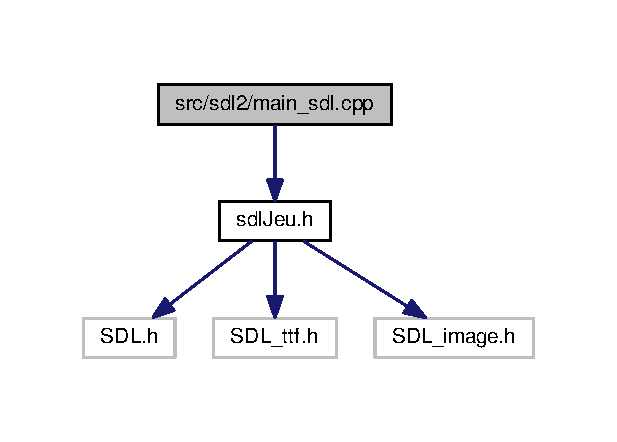
\includegraphics[width=296pt]{main__sdl_8cpp__incl}
\end{center}
\end{figure}
\subsection*{Fonctions}
\begin{DoxyCompactItemize}
\item 
int \hyperlink{main__sdl_8cpp_a3c04138a5bfe5d72780bb7e82a18e627}{main} (int argc, char $\ast$$\ast$argv)
\begin{DoxyCompactList}\small\item\em programme principal pour lancer les fonctions d\textquotesingle{}affichage \end{DoxyCompactList}\end{DoxyCompactItemize}


\subsection{Description détaillée}
Ce fichier contient le programme principal de T\+HE monopoly en S\+D\+L2. 

\begin{DoxyAuthor}{Auteur}
Matthieu Cherrier, Kevin Burdin, Tristan Damian
\end{DoxyAuthor}
\begin{DoxyDate}{Date}
2017/04/20 
\end{DoxyDate}


\subsection{Documentation des fonctions}
\index{main\+\_\+sdl.\+cpp@{main\+\_\+sdl.\+cpp}!main@{main}}
\index{main@{main}!main\+\_\+sdl.\+cpp@{main\+\_\+sdl.\+cpp}}
\subsubsection[{\texorpdfstring{main(int argc, char $\ast$$\ast$argv)}{main(int argc, char **argv)}}]{\setlength{\rightskip}{0pt plus 5cm}int main (
\begin{DoxyParamCaption}
\item[{int}]{argc, }
\item[{char $\ast$$\ast$}]{argv}
\end{DoxyParamCaption}
)}\hypertarget{main__sdl_8cpp_a3c04138a5bfe5d72780bb7e82a18e627}{}\label{main__sdl_8cpp_a3c04138a5bfe5d72780bb7e82a18e627}


programme principal pour lancer les fonctions d\textquotesingle{}affichage 


\begin{DoxyParams}{Paramètres}
{\em argc} & int,argc\+: char$\ast$$\ast$ \\
\hline
\end{DoxyParams}
\begin{DoxyReturn}{Renvoie}
retourne un entier 
\end{DoxyReturn}

\hypertarget{sdlJeu_8cpp}{}\section{Référence du fichier src/sdl2/sdl\+Jeu.cpp}
\label{sdlJeu_8cpp}\index{src/sdl2/sdl\+Jeu.\+cpp@{src/sdl2/sdl\+Jeu.\+cpp}}


Ce fichier contient les fonctions relatives a la gestion de l\textquotesingle{}affichage sdl ainsi qu\textquotesingle{}a la gestion des images.  


{\ttfamily \#include $<$cassert$>$}\\*
{\ttfamily \#include $<$time.\+h$>$}\\*
{\ttfamily \#include \char`\"{}sdl\+Jeu.\+h\char`\"{}}\\*
{\ttfamily \#include $<$stdlib.\+h$>$}\\*
{\ttfamily \#include $<$iostream$>$}\\*
{\ttfamily \#include $<$sstream$>$}\\*
{\ttfamily \#include $<$S\+D\+L.\+h$>$}\\*
{\ttfamily \#include $<$S\+D\+L\+\_\+ttf.\+h$>$}\\*
{\ttfamily \#include $<$S\+D\+L\+\_\+image.\+h$>$}\\*
{\ttfamily \#include $<$S\+D\+L2/\+S\+D\+L\+\_\+image.\+h$>$}\\*
{\ttfamily \#include $<$S\+D\+L2/\+S\+D\+L\+\_\+ttf.\+h$>$}\\*
Graphe des dépendances par inclusion de sdl\+Jeu.\+cpp\+:
\nopagebreak
\begin{figure}[H]
\begin{center}
\leavevmode
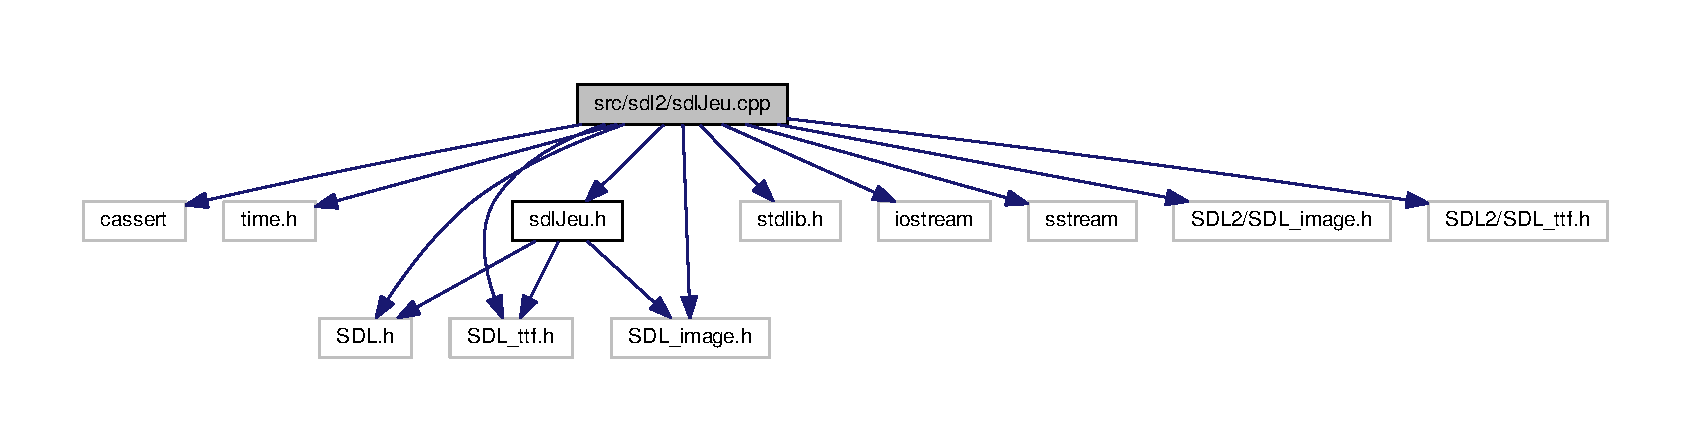
\includegraphics[width=350pt]{sdlJeu_8cpp__incl}
\end{center}
\end{figure}
\subsection*{Fonctions}
\begin{DoxyCompactItemize}
\item 
float {\bfseries temps} ()\hypertarget{sdlJeu_8cpp_a81d5aa8ff5cf87d329a39cb4d2f44c73}{}\label{sdlJeu_8cpp_a81d5aa8ff5cf87d329a39cb4d2f44c73}

\end{DoxyCompactItemize}
\subsection*{Variables}
\begin{DoxyCompactItemize}
\item 
const int {\bfseries T\+A\+I\+L\+L\+E\+\_\+\+S\+P\+R\+I\+TE} = 12\hypertarget{sdlJeu_8cpp_a6c3723683dfe1e0731a0f01ebc2e84f9}{}\label{sdlJeu_8cpp_a6c3723683dfe1e0731a0f01ebc2e84f9}

\item 
const int {\bfseries T\+A\+I\+L\+L\+E\+\_\+\+C\+A\+S\+EX} = 65\hypertarget{sdlJeu_8cpp_af7240774ad5a532b73540a58f40748c7}{}\label{sdlJeu_8cpp_af7240774ad5a532b73540a58f40748c7}

\item 
const int {\bfseries T\+A\+I\+L\+L\+E\+\_\+\+C\+A\+S\+EY} = 58\hypertarget{sdlJeu_8cpp_a06692fce21851180c94be2e116f0fca6}{}\label{sdlJeu_8cpp_a06692fce21851180c94be2e116f0fca6}

\end{DoxyCompactItemize}


\subsection{Description détaillée}
Ce fichier contient les fonctions relatives a la gestion de l\textquotesingle{}affichage sdl ainsi qu\textquotesingle{}a la gestion des images. 

\begin{DoxyAuthor}{Auteur}
Matthieu Cherrier, Kevin Burdin, Tristan Damian
\end{DoxyAuthor}
\begin{DoxyDate}{Date}
2017/04/20 
\end{DoxyDate}

\hypertarget{sdlJeu_8h}{}\section{Référence du fichier src/sdl2/sdl\+Jeu.h}
\label{sdlJeu_8h}\index{src/sdl2/sdl\+Jeu.\+h@{src/sdl2/sdl\+Jeu.\+h}}


Ce fichier contient les en-\/tetes des fonctions relatives a la gestion de l\textquotesingle{}affichage sdl ainsi qu\textquotesingle{}a la gestion des images.  


{\ttfamily \#include $<$S\+D\+L.\+h$>$}\\*
{\ttfamily \#include $<$S\+D\+L\+\_\+ttf.\+h$>$}\\*
{\ttfamily \#include $<$S\+D\+L\+\_\+image.\+h$>$}\\*
Graphe des dépendances par inclusion de sdl\+Jeu.\+h\+:
\nopagebreak
\begin{figure}[H]
\begin{center}
\leavevmode
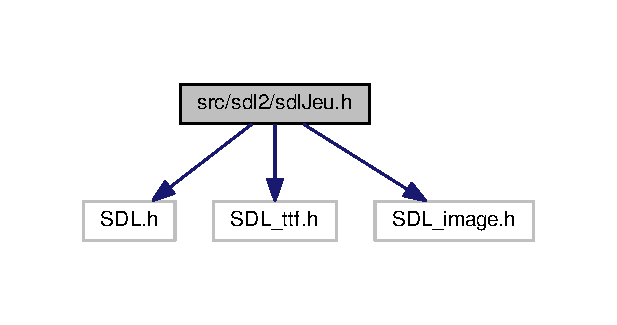
\includegraphics[width=296pt]{sdlJeu_8h__incl}
\end{center}
\end{figure}
Ce graphe montre quels fichiers incluent directement ou indirectement ce fichier \+:
\nopagebreak
\begin{figure}[H]
\begin{center}
\leavevmode
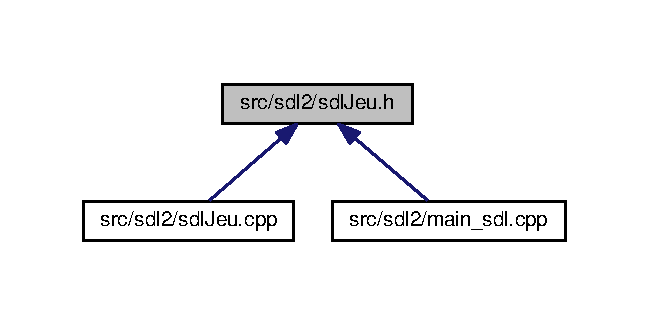
\includegraphics[width=312pt]{sdlJeu_8h__dep__incl}
\end{center}
\end{figure}
\subsection*{Classes}
\begin{DoxyCompactItemize}
\item 
class \hyperlink{classImage}{Image}
\begin{DoxyCompactList}\small\item\em Pour g�rer une image avec S\+D\+L2. \end{DoxyCompactList}\item 
class \hyperlink{classsdlJeu}{sdl\+Jeu}
\end{DoxyCompactItemize}


\subsection{Description détaillée}
Ce fichier contient les en-\/tetes des fonctions relatives a la gestion de l\textquotesingle{}affichage sdl ainsi qu\textquotesingle{}a la gestion des images. 

\begin{DoxyAuthor}{Auteur}
Matthieu Cherrier, Kevin Burdin, Tristan Damian
\end{DoxyAuthor}
\begin{DoxyDate}{Date}
2017/04/20 
\end{DoxyDate}

\hypertarget{Carte_8cpp}{}\section{Référence du fichier src/txt/\+Carte.cpp}
\label{Carte_8cpp}\index{src/txt/\+Carte.\+cpp@{src/txt/\+Carte.\+cpp}}


Ce fichier contient les fonctions relatives a la gestion des cartes.  


{\ttfamily \#include $<$string$>$}\\*
{\ttfamily \#include $<$iostream$>$}\\*
{\ttfamily \#include \char`\"{}Carte.\+h\char`\"{}}\\*
{\ttfamily \#include \char`\"{}Jeu.\+h\char`\"{}}\\*
{\ttfamily \#include \char`\"{}Paquet\+Caisse\+Comm.\+h\char`\"{}}\\*
{\ttfamily \#include \char`\"{}Paquet\+Chance.\+h\char`\"{}}\\*
Graphe des dépendances par inclusion de Carte.\+cpp\+:
\nopagebreak
\begin{figure}[H]
\begin{center}
\leavevmode
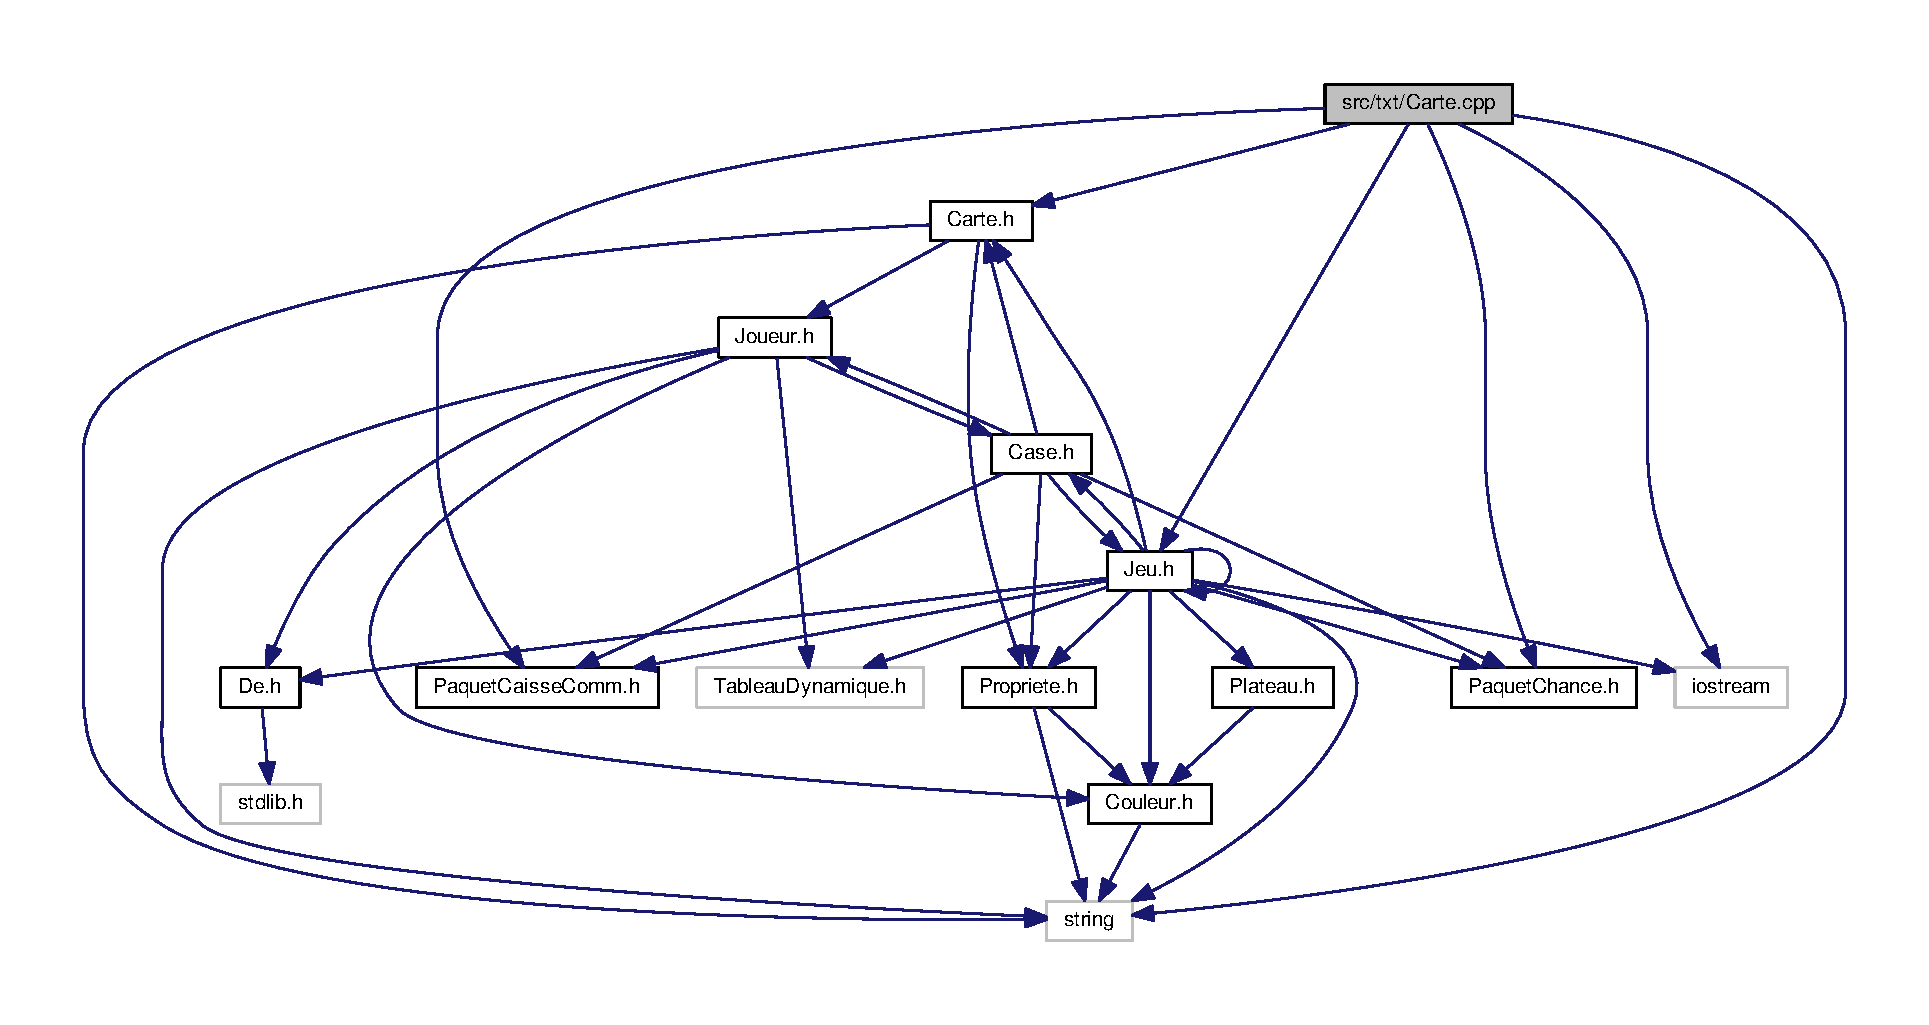
\includegraphics[width=350pt]{Carte_8cpp__incl}
\end{center}
\end{figure}


\subsection{Description détaillée}
Ce fichier contient les fonctions relatives a la gestion des cartes. 

\begin{DoxyAuthor}{Auteur}
Matthieu Cherrier, Kevin Burdin, Tristan Damian
\end{DoxyAuthor}
\begin{DoxyDate}{Date}
2017/04/20 
\end{DoxyDate}

\hypertarget{Carte_8h}{}\section{Référence du fichier src/txt/\+Carte.h}
\label{Carte_8h}\index{src/txt/\+Carte.\+h@{src/txt/\+Carte.\+h}}


Ce fichier contient les en-\/tetes des fonctions relatives a la gestion des cartes.  


{\ttfamily \#include $<$string$>$}\\*
{\ttfamily \#include \char`\"{}Joueur.\+h\char`\"{}}\\*
Graphe des dépendances par inclusion de Carte.\+h\+:
\nopagebreak
\begin{figure}[H]
\begin{center}
\leavevmode
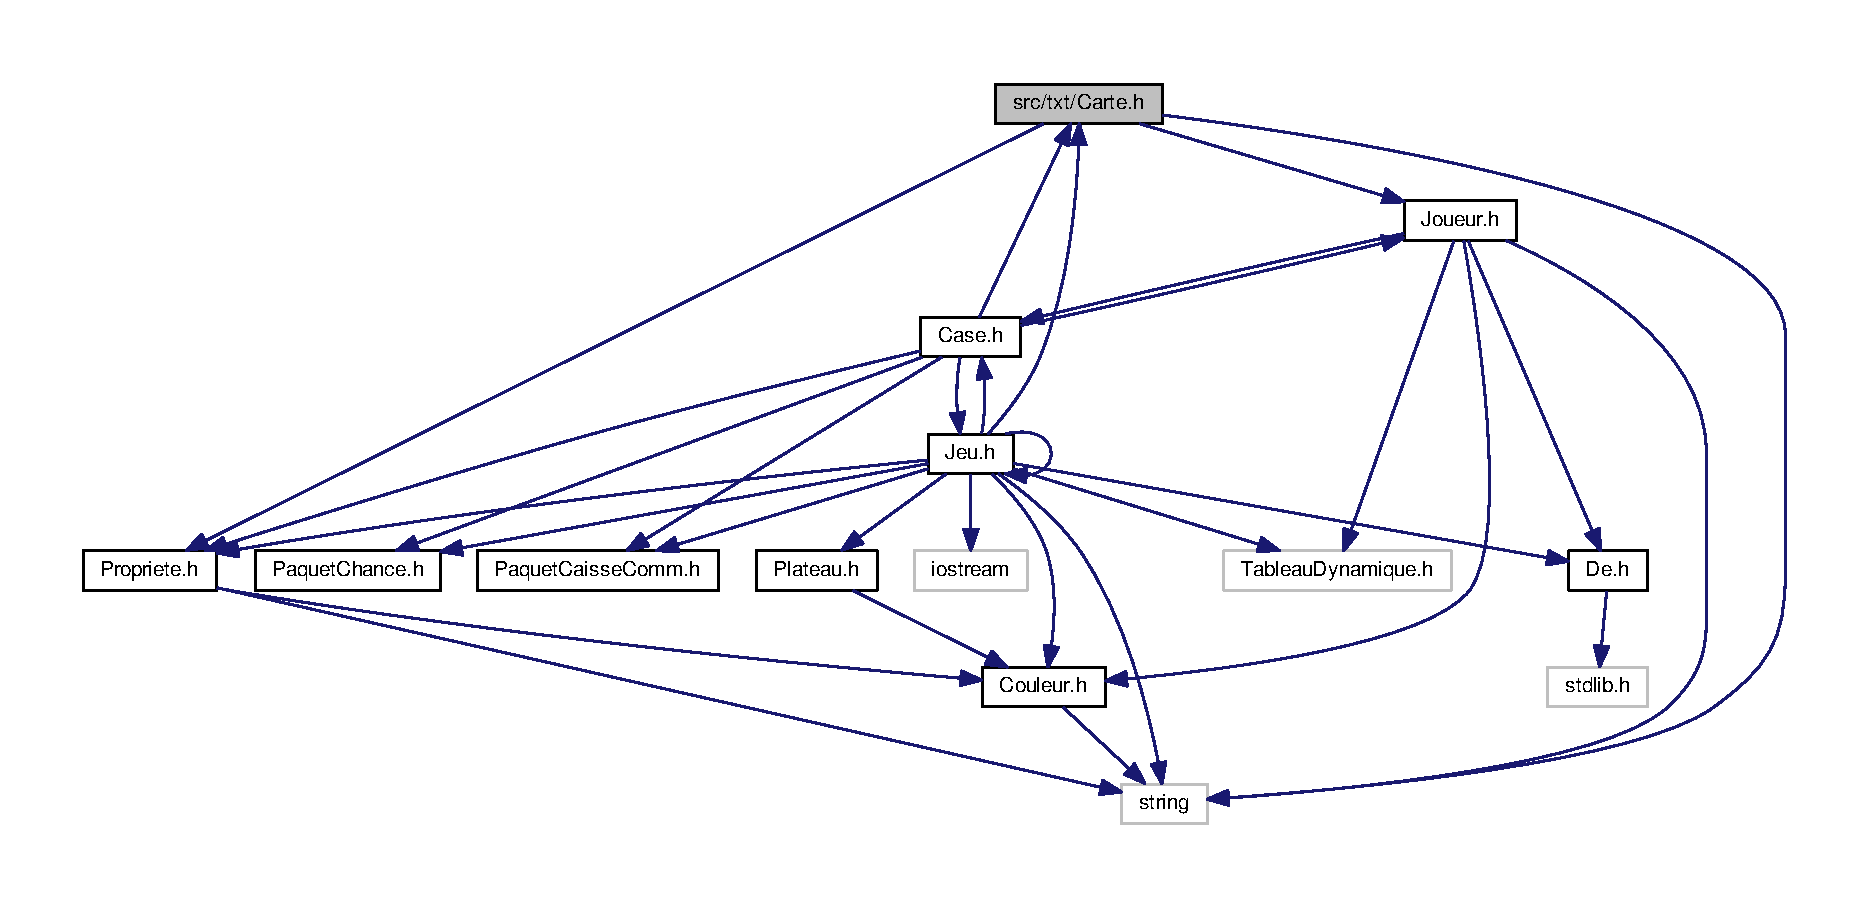
\includegraphics[width=350pt]{Carte_8h__incl}
\end{center}
\end{figure}
Ce graphe montre quels fichiers incluent directement ou indirectement ce fichier \+:
\nopagebreak
\begin{figure}[H]
\begin{center}
\leavevmode
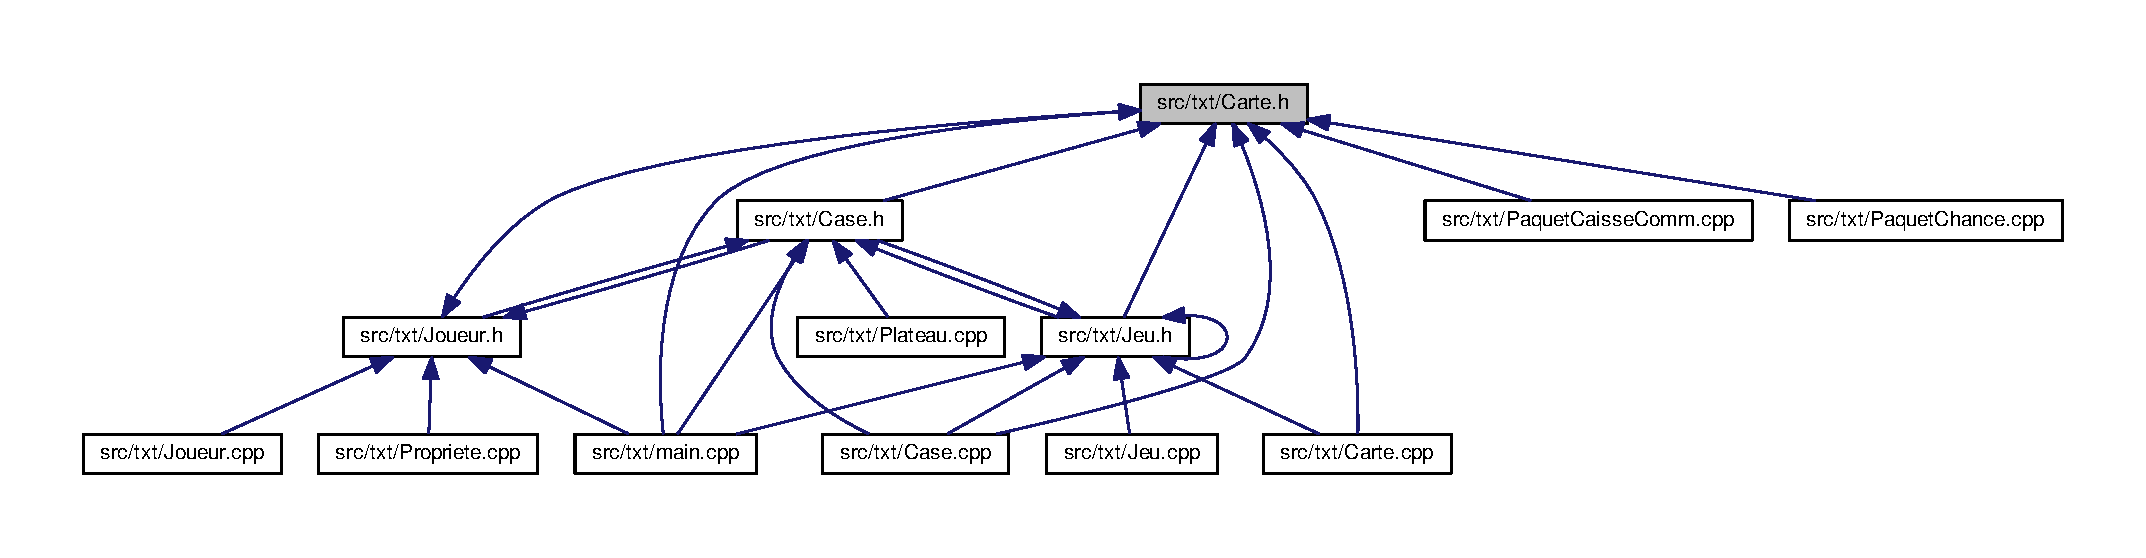
\includegraphics[width=350pt]{Carte_8h__dep__incl}
\end{center}
\end{figure}
\subsection*{Classes}
\begin{DoxyCompactItemize}
\item 
class \hyperlink{classCarte}{Carte}
\end{DoxyCompactItemize}


\subsection{Description détaillée}
Ce fichier contient les en-\/tetes des fonctions relatives a la gestion des cartes. 

\begin{DoxyAuthor}{Auteur}
Matthieu Cherrier, Kevin Burdin, Tristan Damian
\end{DoxyAuthor}
\begin{DoxyDate}{Date}
2017/04/20 
\end{DoxyDate}

\hypertarget{Case_8cpp}{}\section{Référence du fichier src/txt/\+Case.cpp}
\label{Case_8cpp}\index{src/txt/\+Case.\+cpp@{src/txt/\+Case.\+cpp}}


Ce fichier contient les fonctions relatives a la gestion des cases.  


{\ttfamily \#include \char`\"{}Case.\+h\char`\"{}}\\*
{\ttfamily \#include \char`\"{}Carte.\+h\char`\"{}}\\*
{\ttfamily \#include \char`\"{}Paquet\+Caisse\+Comm.\+h\char`\"{}}\\*
{\ttfamily \#include \char`\"{}Paquet\+Chance.\+h\char`\"{}}\\*
{\ttfamily \#include \char`\"{}Jeu.\+h\char`\"{}}\\*
{\ttfamily \#include $<$iostream$>$}\\*
Graphe des dépendances par inclusion de Case.\+cpp\+:
\nopagebreak
\begin{figure}[H]
\begin{center}
\leavevmode
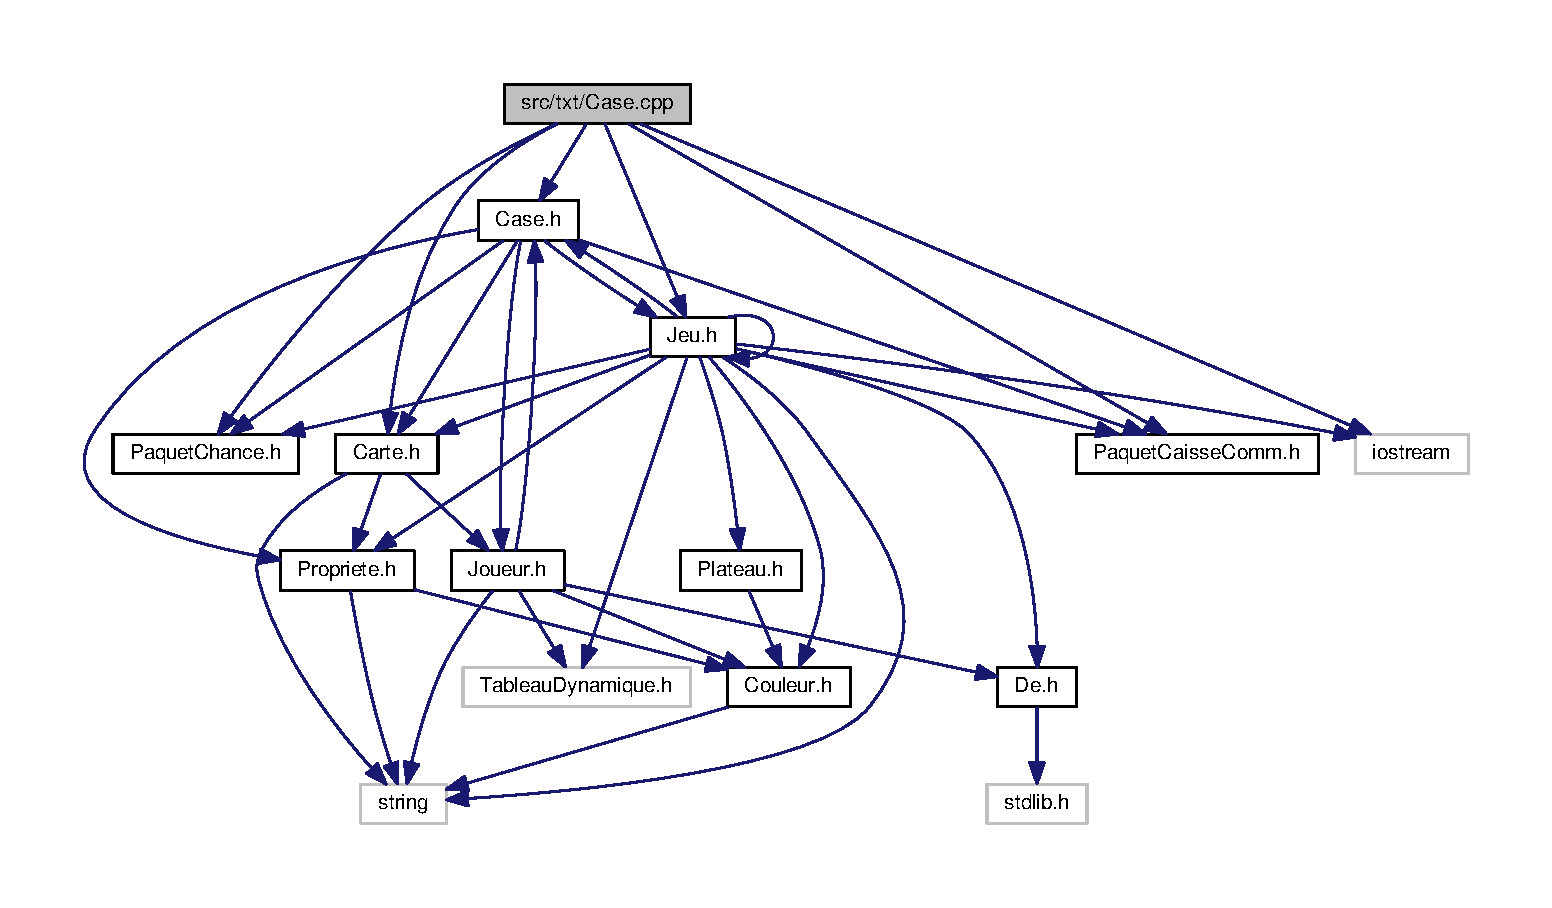
\includegraphics[width=350pt]{Case_8cpp__incl}
\end{center}
\end{figure}


\subsection{Description détaillée}
Ce fichier contient les fonctions relatives a la gestion des cases. 

\begin{DoxyAuthor}{Auteur}
Matthieu Cherrier, Kevin Burdin, Tristan Damian
\end{DoxyAuthor}
\begin{DoxyDate}{Date}
2017/04/20 
\end{DoxyDate}

\hypertarget{Case_8h}{}\section{Référence du fichier src/txt/\+Case.h}
\label{Case_8h}\index{src/txt/\+Case.\+h@{src/txt/\+Case.\+h}}


Ce fichier contient les en-\/tetes des fonctions relatives a la gestion des cases.  


{\ttfamily \#include \char`\"{}Propriete.\+h\char`\"{}}\\*
{\ttfamily \#include \char`\"{}Carte.\+h\char`\"{}}\\*
{\ttfamily \#include \char`\"{}Paquet\+Caisse\+Comm.\+h\char`\"{}}\\*
{\ttfamily \#include \char`\"{}Paquet\+Chance.\+h\char`\"{}}\\*
{\ttfamily \#include \char`\"{}Joueur.\+h\char`\"{}}\\*
{\ttfamily \#include \char`\"{}Jeu.\+h\char`\"{}}\\*
Graphe des dépendances par inclusion de Case.\+h\+:
\nopagebreak
\begin{figure}[H]
\begin{center}
\leavevmode
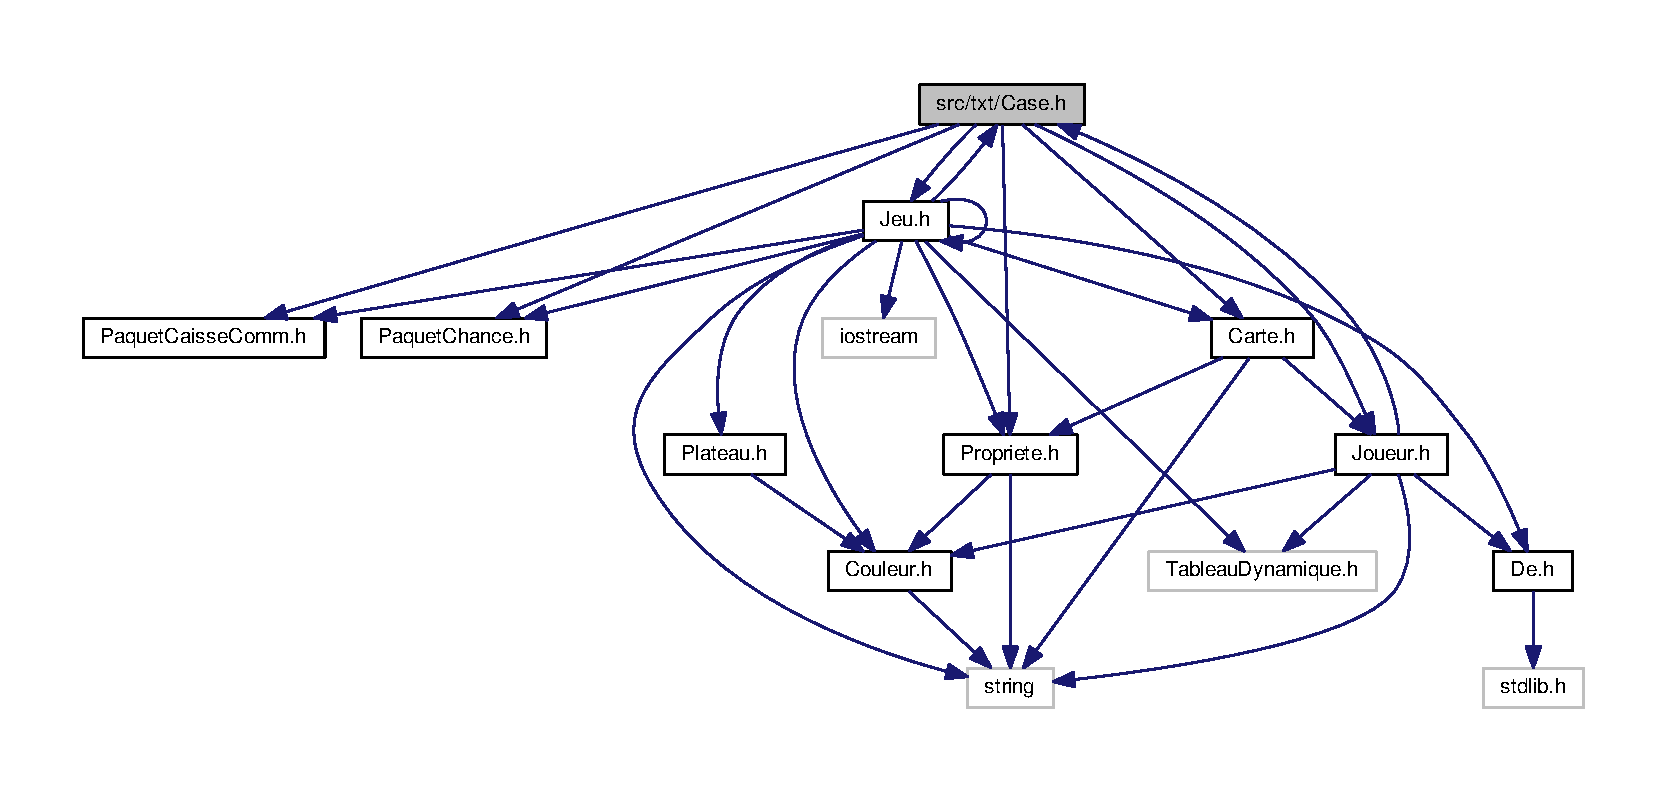
\includegraphics[width=350pt]{Case_8h__incl}
\end{center}
\end{figure}
Ce graphe montre quels fichiers incluent directement ou indirectement ce fichier \+:
\nopagebreak
\begin{figure}[H]
\begin{center}
\leavevmode
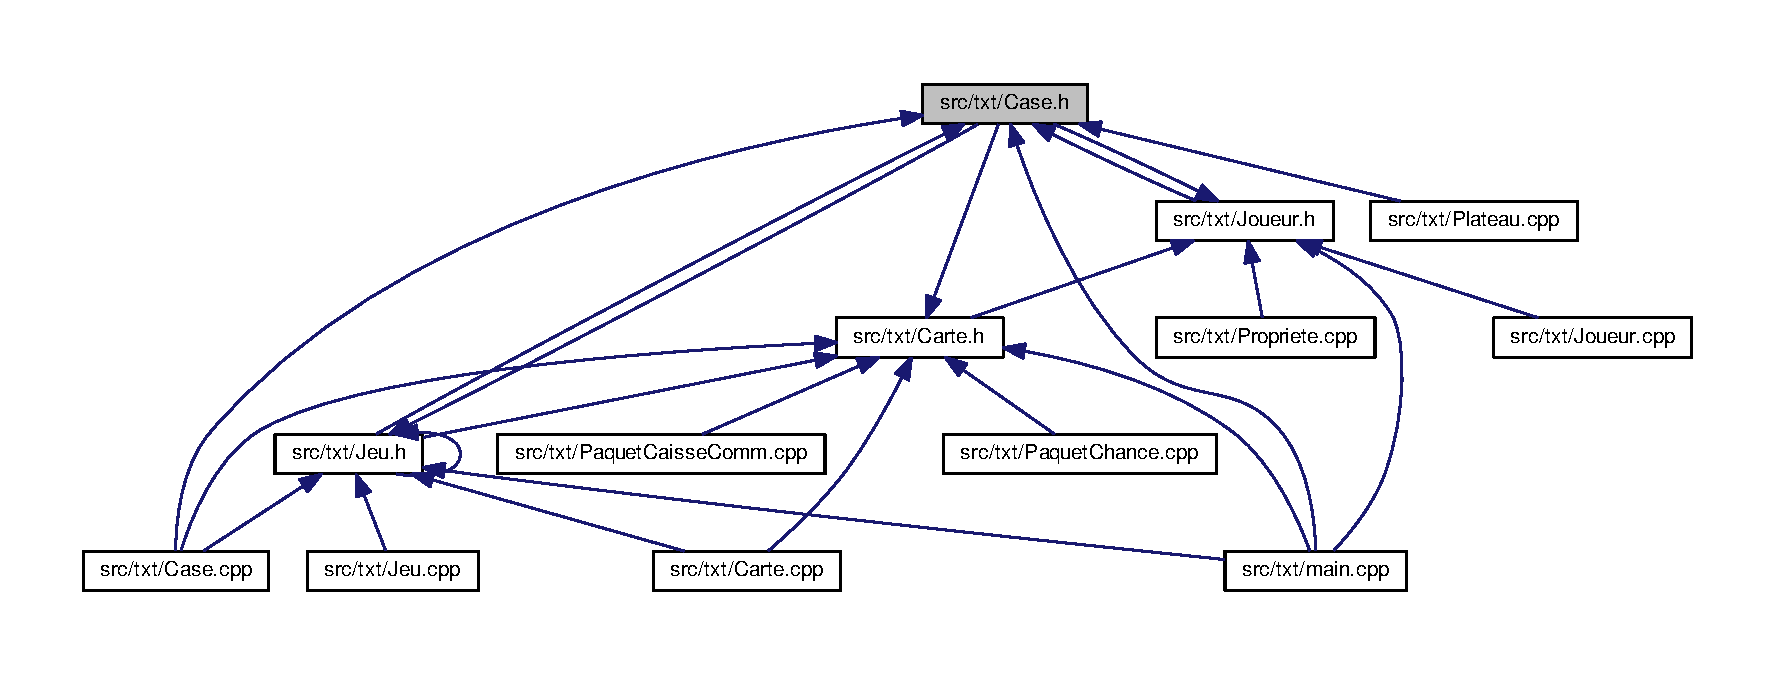
\includegraphics[width=350pt]{Case_8h__dep__incl}
\end{center}
\end{figure}
\subsection*{Classes}
\begin{DoxyCompactItemize}
\item 
class \hyperlink{classCase}{Case}
\end{DoxyCompactItemize}


\subsection{Description détaillée}
Ce fichier contient les en-\/tetes des fonctions relatives a la gestion des cases. 

\begin{DoxyAuthor}{Auteur}
Matthieu Cherrier, Kevin Burdin, Tristan Damian
\end{DoxyAuthor}
\begin{DoxyDate}{Date}
2017/04/20 
\end{DoxyDate}

\hypertarget{Couleur_8cpp}{}\section{Référence du fichier src/txt/\+Couleur.cpp}
\label{Couleur_8cpp}\index{src/txt/\+Couleur.\+cpp@{src/txt/\+Couleur.\+cpp}}


Ce fichier contient les fonctions relatives a la gestion des couleurs.  


{\ttfamily \#include \char`\"{}Couleur.\+h\char`\"{}}\\*
{\ttfamily \#include $<$assert.\+h$>$}\\*
{\ttfamily \#include $<$iostream$>$}\\*
Graphe des dépendances par inclusion de Couleur.\+cpp\+:
\nopagebreak
\begin{figure}[H]
\begin{center}
\leavevmode
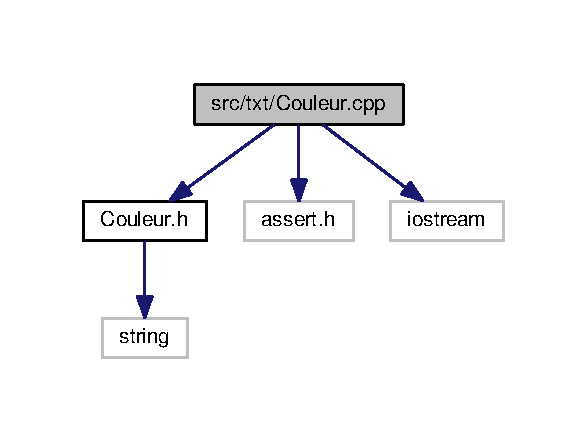
\includegraphics[width=282pt]{Couleur_8cpp__incl}
\end{center}
\end{figure}


\subsection{Description détaillée}
Ce fichier contient les fonctions relatives a la gestion des couleurs. 

\begin{DoxyAuthor}{Auteur}
Matthieu Cherrier, Kevin Burdin, Tristan Damian
\end{DoxyAuthor}
\begin{DoxyDate}{Date}
2017/04/20 
\end{DoxyDate}

\hypertarget{Couleur_8h}{}\section{Référence du fichier src/txt/\+Couleur.h}
\label{Couleur_8h}\index{src/txt/\+Couleur.\+h@{src/txt/\+Couleur.\+h}}


Ce fichier contient les en-\/tetes des fonctions relatives a la gestion des couleurs.  


{\ttfamily \#include $<$string$>$}\\*
Graphe des dépendances par inclusion de Couleur.\+h\+:
\nopagebreak
\begin{figure}[H]
\begin{center}
\leavevmode
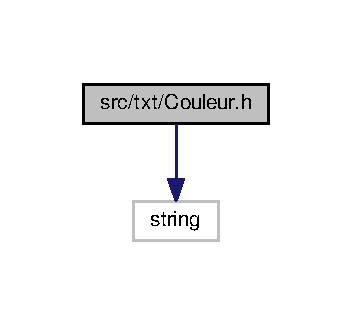
\includegraphics[width=169pt]{Couleur_8h__incl}
\end{center}
\end{figure}
Ce graphe montre quels fichiers incluent directement ou indirectement ce fichier \+:
\nopagebreak
\begin{figure}[H]
\begin{center}
\leavevmode
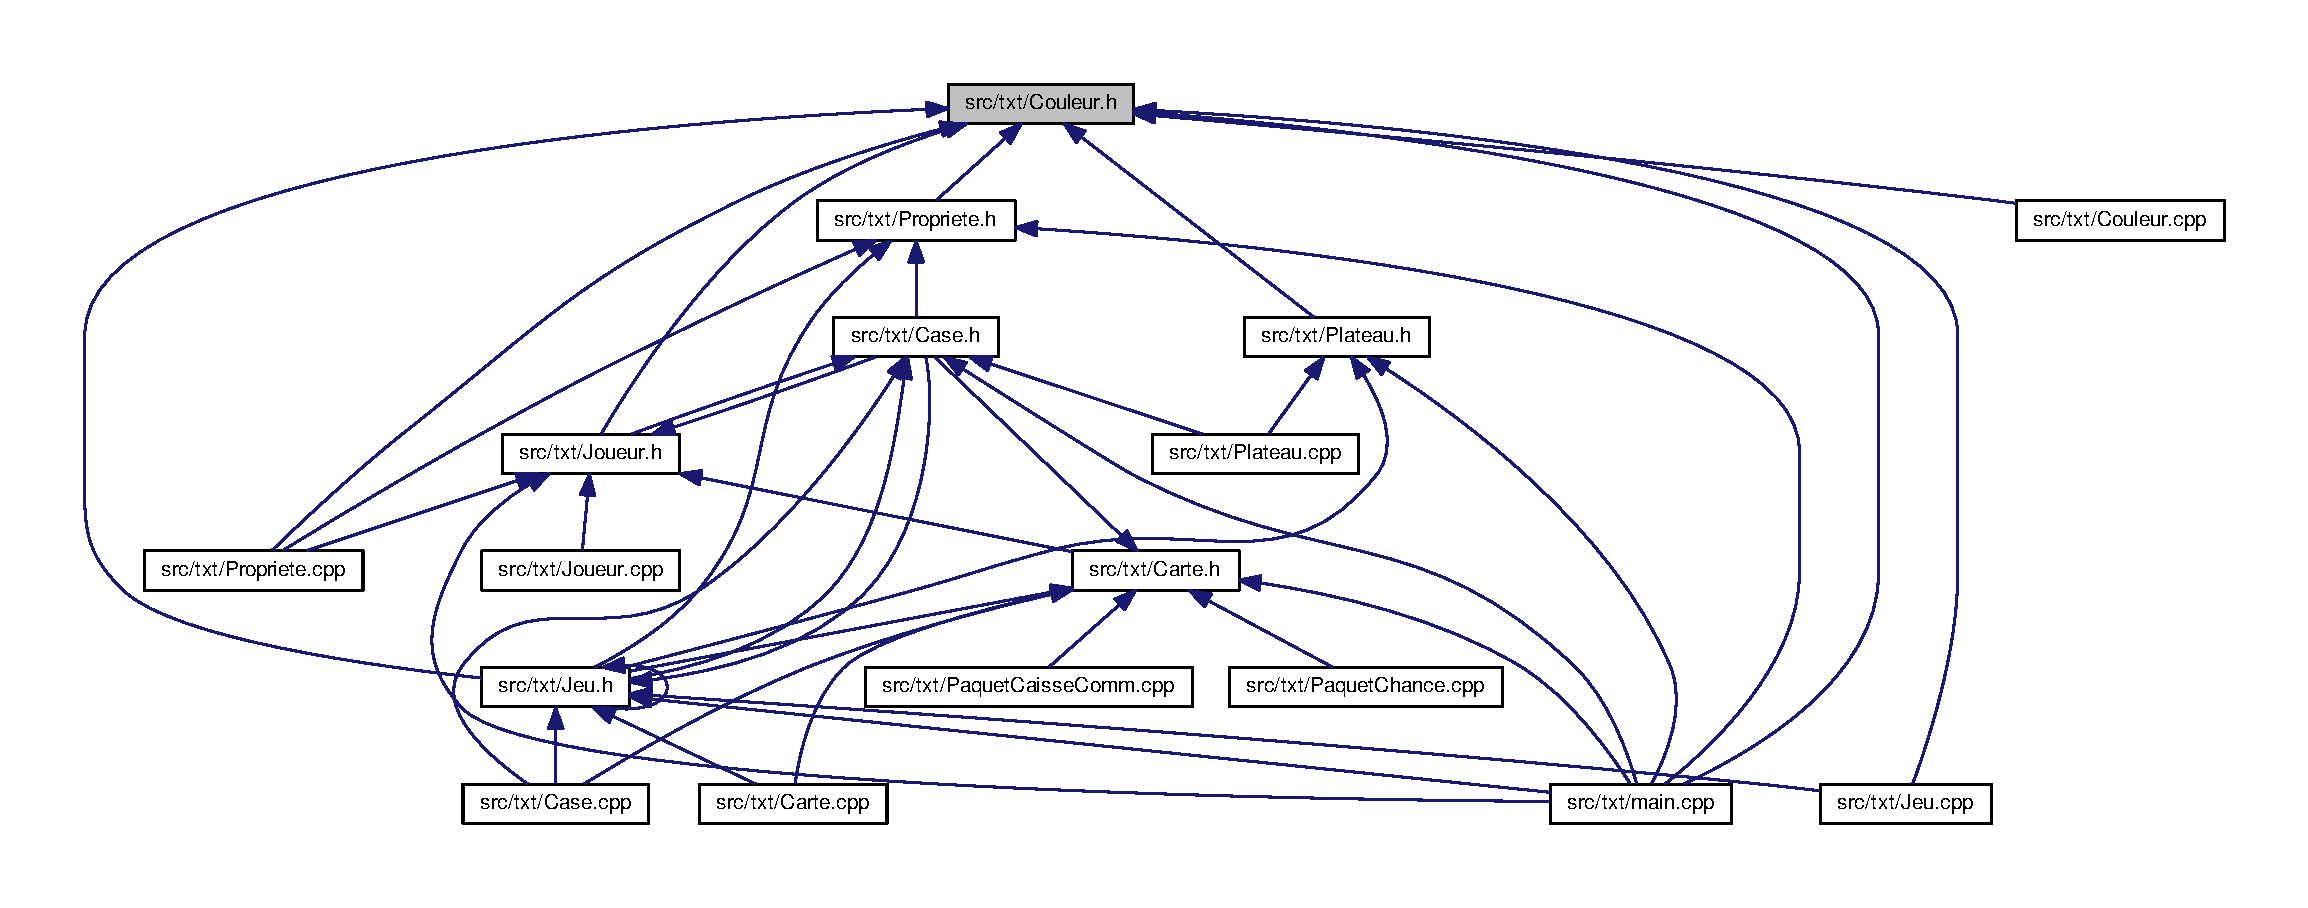
\includegraphics[width=350pt]{Couleur_8h__dep__incl}
\end{center}
\end{figure}
\subsection*{Classes}
\begin{DoxyCompactItemize}
\item 
class \hyperlink{classCouleur}{Couleur}
\end{DoxyCompactItemize}


\subsection{Description détaillée}
Ce fichier contient les en-\/tetes des fonctions relatives a la gestion des couleurs. 

\begin{DoxyAuthor}{Auteur}
Matthieu Cherrier, Kevin Burdin, Tristan Damian
\end{DoxyAuthor}
\begin{DoxyDate}{Date}
2017/04/20 
\end{DoxyDate}

\hypertarget{De_8cpp}{}\section{Référence du fichier src/txt/\+De.cpp}
\label{De_8cpp}\index{src/txt/\+De.\+cpp@{src/txt/\+De.\+cpp}}


Ce fichier contient les fonctions relatives a la gestion des d��s.  


{\ttfamily \#include \char`\"{}De.\+h\char`\"{}}\\*
{\ttfamily \#include $<$cstdlib$>$}\\*
{\ttfamily \#include $<$time.\+h$>$}\\*
{\ttfamily \#include $<$iostream$>$}\\*
Graphe des dépendances par inclusion de De.\+cpp\+:
\nopagebreak
\begin{figure}[H]
\begin{center}
\leavevmode
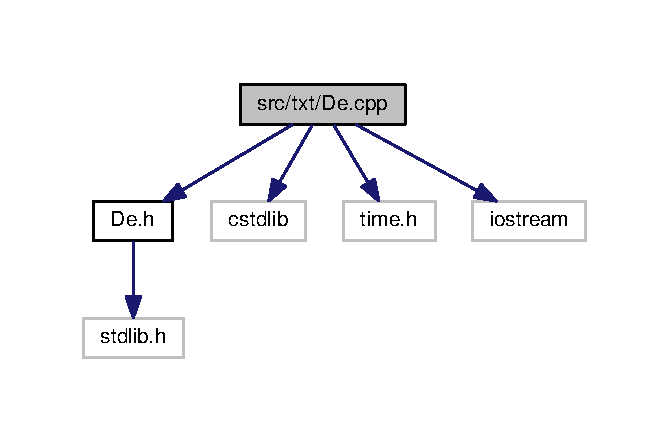
\includegraphics[width=321pt]{De_8cpp__incl}
\end{center}
\end{figure}


\subsection{Description détaillée}
Ce fichier contient les fonctions relatives a la gestion des d��s. 

\begin{DoxyAuthor}{Auteur}
Matthieu Cherrier, Kevin Burdin, Tristan Damian
\end{DoxyAuthor}
\begin{DoxyDate}{Date}
2017/04/20 
\end{DoxyDate}

\hypertarget{De_8h}{}\section{Référence du fichier src/txt/\+De.h}
\label{De_8h}\index{src/txt/\+De.\+h@{src/txt/\+De.\+h}}


Ce fichier contient les en-\/tetes des fonctions relatives a la gestion des d��s.  


{\ttfamily \#include $<$stdlib.\+h$>$}\\*
Graphe des dépendances par inclusion de De.\+h\+:
\nopagebreak
\begin{figure}[H]
\begin{center}
\leavevmode
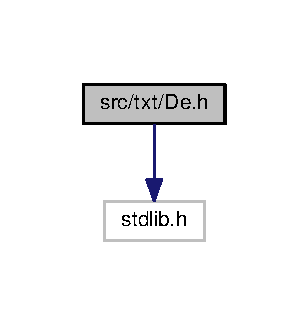
\includegraphics[width=148pt]{De_8h__incl}
\end{center}
\end{figure}
Ce graphe montre quels fichiers incluent directement ou indirectement ce fichier \+:
\nopagebreak
\begin{figure}[H]
\begin{center}
\leavevmode
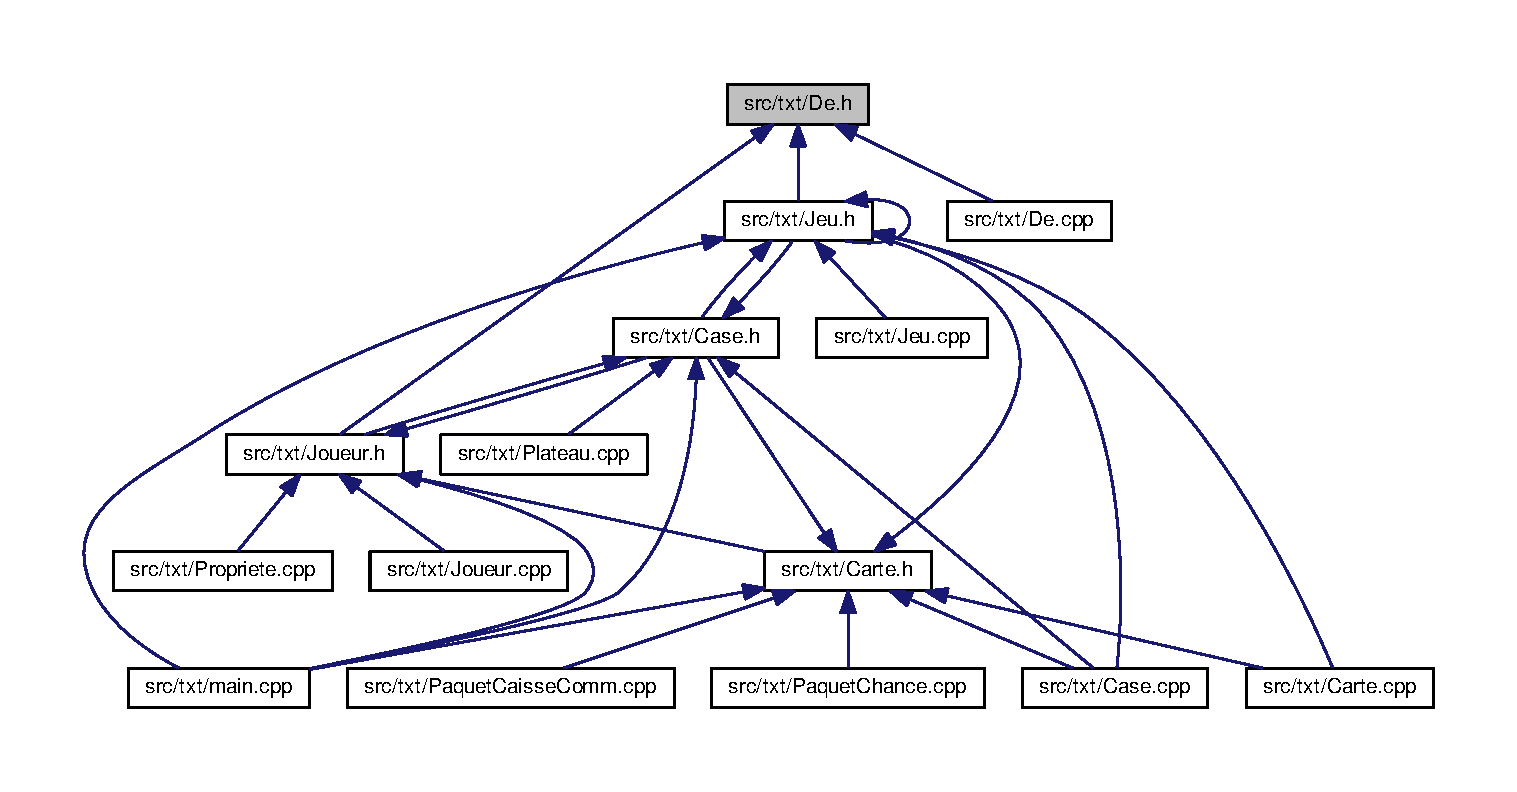
\includegraphics[width=350pt]{De_8h__dep__incl}
\end{center}
\end{figure}
\subsection*{Classes}
\begin{DoxyCompactItemize}
\item 
class \hyperlink{classDe}{De}
\end{DoxyCompactItemize}


\subsection{Description détaillée}
Ce fichier contient les en-\/tetes des fonctions relatives a la gestion des d��s. 

\begin{DoxyAuthor}{Auteur}
Matthieu Cherrier, Kevin Burdin, Tristan Damian
\end{DoxyAuthor}
\begin{DoxyDate}{Date}
2017/04/20 
\end{DoxyDate}

\hypertarget{Jeu_8cpp}{}\section{Référence du fichier src/txt/\+Jeu.cpp}
\label{Jeu_8cpp}\index{src/txt/\+Jeu.\+cpp@{src/txt/\+Jeu.\+cpp}}


Ce fichier contient les fonctions pour initialiser et gerer le jeu.  


{\ttfamily \#include \char`\"{}Jeu.\+h\char`\"{}}\\*
{\ttfamily \#include \char`\"{}Couleur.\+h\char`\"{}}\\*
{\ttfamily \#include $<$typeinfo$>$}\\*
{\ttfamily \#include $<$iostream$>$}\\*
{\ttfamily \#include $<$string$>$}\\*
Graphe des dépendances par inclusion de Jeu.\+cpp\+:
\nopagebreak
\begin{figure}[H]
\begin{center}
\leavevmode
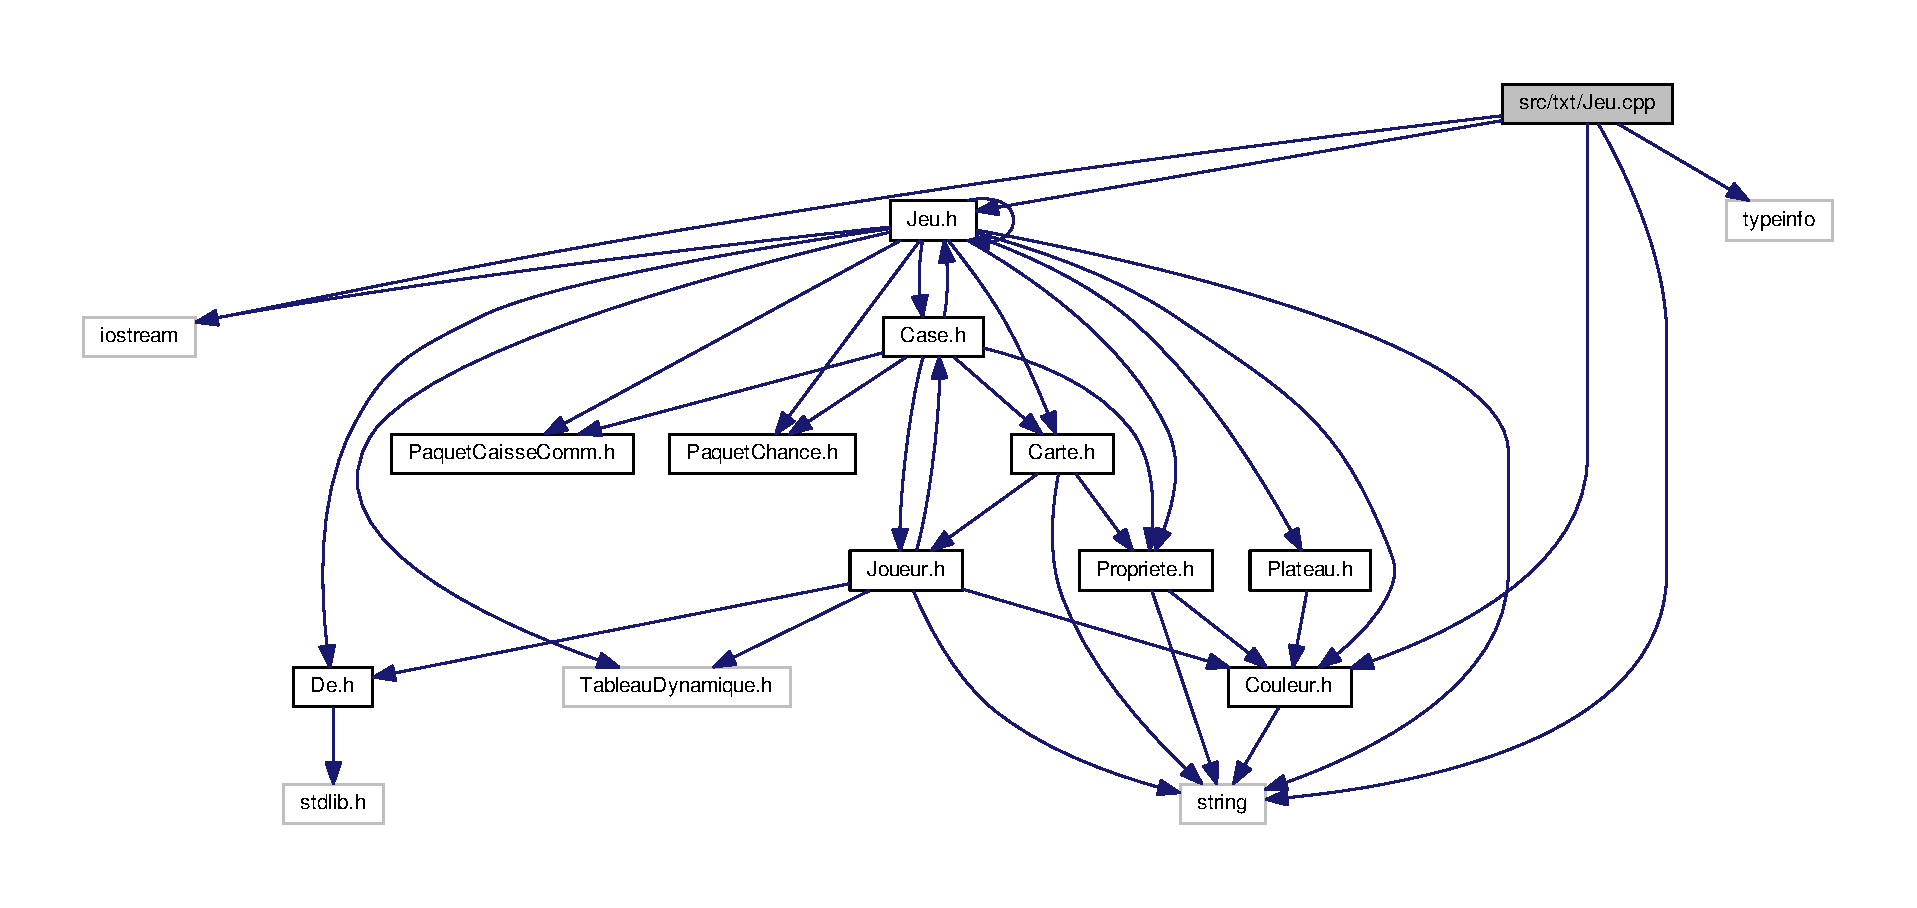
\includegraphics[width=350pt]{Jeu_8cpp__incl}
\end{center}
\end{figure}


\subsection{Description détaillée}
Ce fichier contient les fonctions pour initialiser et gerer le jeu. 

\begin{DoxyAuthor}{Auteur}
Matthieu Cherrier, Kevin Burdin, Tristan Damian
\end{DoxyAuthor}
\begin{DoxyDate}{Date}
2017/04/20 
\end{DoxyDate}

\hypertarget{Jeu_8h}{}\section{Référence du fichier src/txt/\+Jeu.h}
\label{Jeu_8h}\index{src/txt/\+Jeu.\+h@{src/txt/\+Jeu.\+h}}


Ce fichier contient les en-\/tetes des fonctions pour initialiser et gerer le jeu.  


{\ttfamily \#include $<$iostream$>$}\\*
{\ttfamily \#include $<$string$>$}\\*
{\ttfamily \#include \char`\"{}Couleur.\+h\char`\"{}}\\*
{\ttfamily \#include \char`\"{}Case.\+h\char`\"{}}\\*
{\ttfamily \#include \char`\"{}Plateau.\+h\char`\"{}}\\*
{\ttfamily \#include \char`\"{}Propriete.\+h\char`\"{}}\\*
{\ttfamily \#include \char`\"{}Carte.\+h\char`\"{}}\\*
{\ttfamily \#include \char`\"{}Jeu.\+h\char`\"{}}\\*
{\ttfamily \#include \char`\"{}Paquet\+Chance.\+h\char`\"{}}\\*
{\ttfamily \#include \char`\"{}Paquet\+Caisse\+Comm.\+h\char`\"{}}\\*
{\ttfamily \#include \char`\"{}De.\+h\char`\"{}}\\*
{\ttfamily \#include \char`\"{}Tableau\+Dynamique.\+h\char`\"{}}\\*
Graphe des dépendances par inclusion de Jeu.\+h\+:
\nopagebreak
\begin{figure}[H]
\begin{center}
\leavevmode
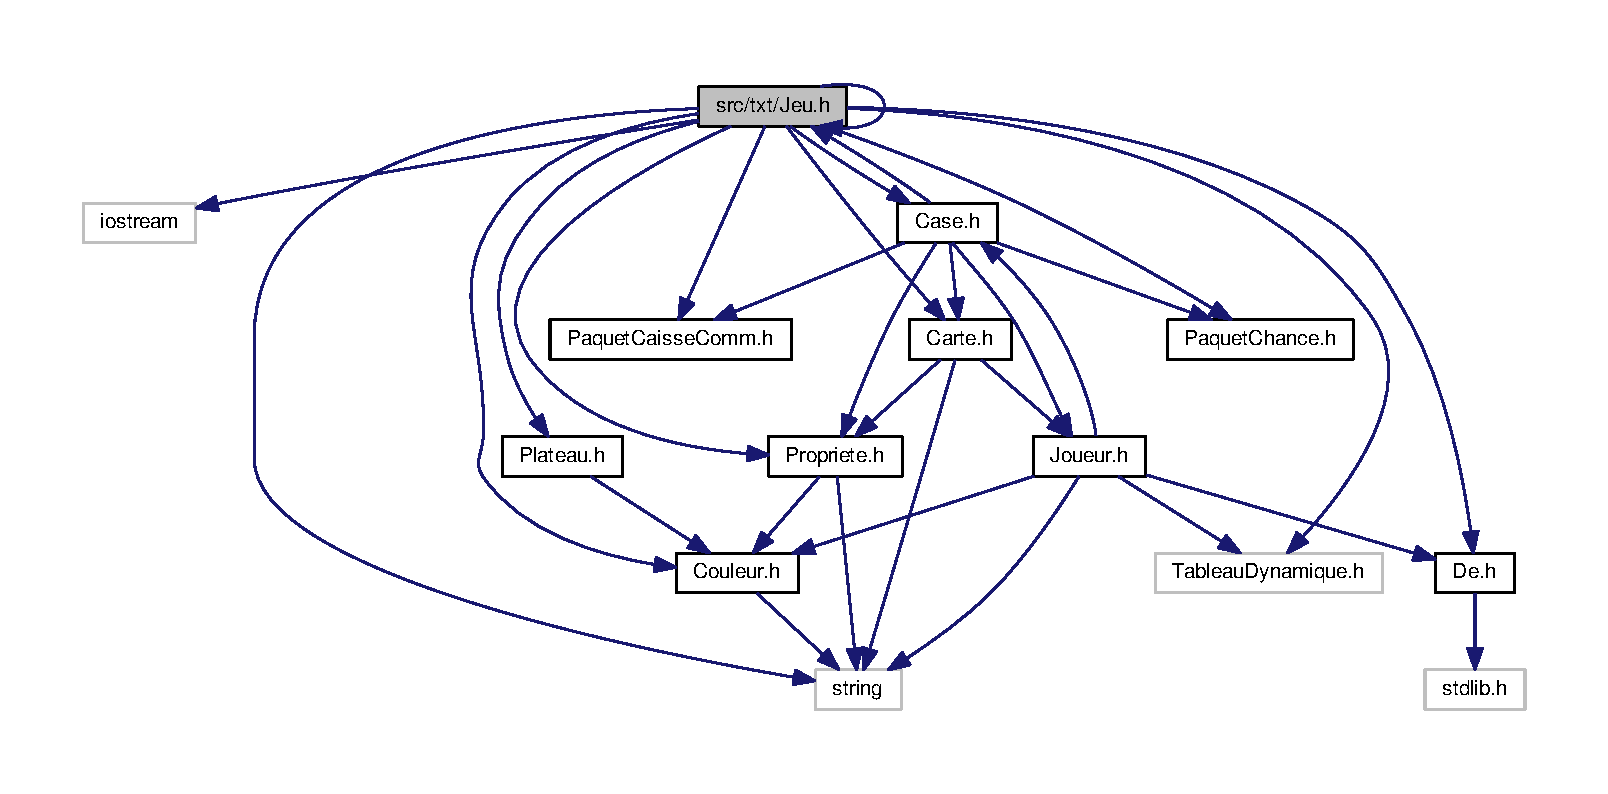
\includegraphics[width=350pt]{Jeu_8h__incl}
\end{center}
\end{figure}
Ce graphe montre quels fichiers incluent directement ou indirectement ce fichier \+:
\nopagebreak
\begin{figure}[H]
\begin{center}
\leavevmode
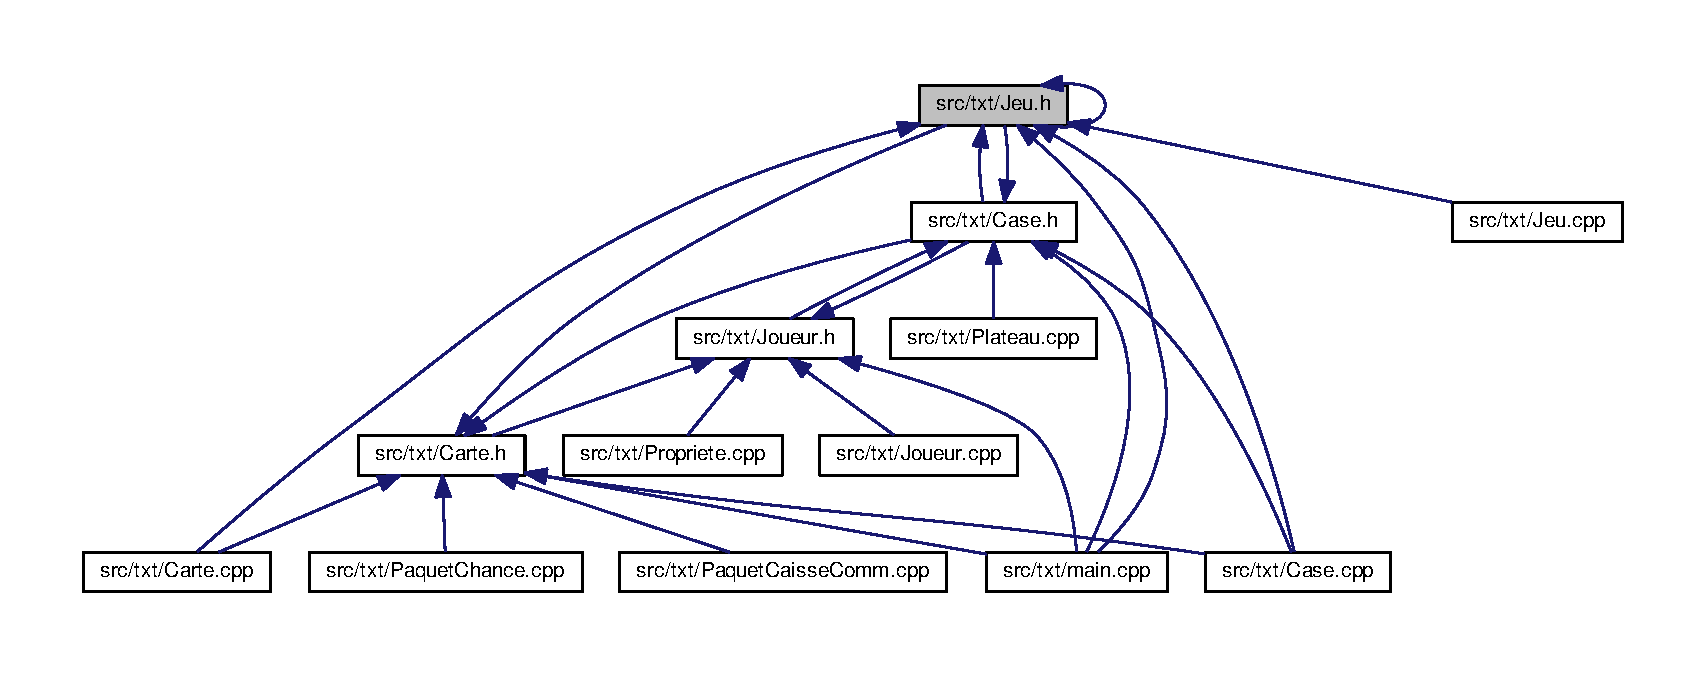
\includegraphics[width=350pt]{Jeu_8h__dep__incl}
\end{center}
\end{figure}
\subsection*{Classes}
\begin{DoxyCompactItemize}
\item 
class \hyperlink{classJeu}{Jeu}
\end{DoxyCompactItemize}


\subsection{Description détaillée}
Ce fichier contient les en-\/tetes des fonctions pour initialiser et gerer le jeu. 

\begin{DoxyAuthor}{Auteur}
Matthieu Cherrier, Kevin Burdin, Tristan Damian
\end{DoxyAuthor}
\begin{DoxyDate}{Date}
2017/04/20 
\end{DoxyDate}

\hypertarget{Joueur_8cpp}{}\section{Référence du fichier src/txt/\+Joueur.cpp}
\label{Joueur_8cpp}\index{src/txt/\+Joueur.\+cpp@{src/txt/\+Joueur.\+cpp}}


Ce fichier gere les caracteristiques des joueurs ainsi que leurs actions.  


{\ttfamily \#include \char`\"{}Joueur.\+h\char`\"{}}\\*
{\ttfamily \#include $<$string$>$}\\*
{\ttfamily \#include $<$iostream$>$}\\*
{\ttfamily \#include $<$typeinfo$>$}\\*
{\ttfamily \#include $<$assert.\+h$>$}\\*
{\ttfamily \#include \char`\"{}Tableau\+Dynamique.\+h\char`\"{}}\\*
Graphe des dépendances par inclusion de Joueur.\+cpp\+:
\nopagebreak
\begin{figure}[H]
\begin{center}
\leavevmode
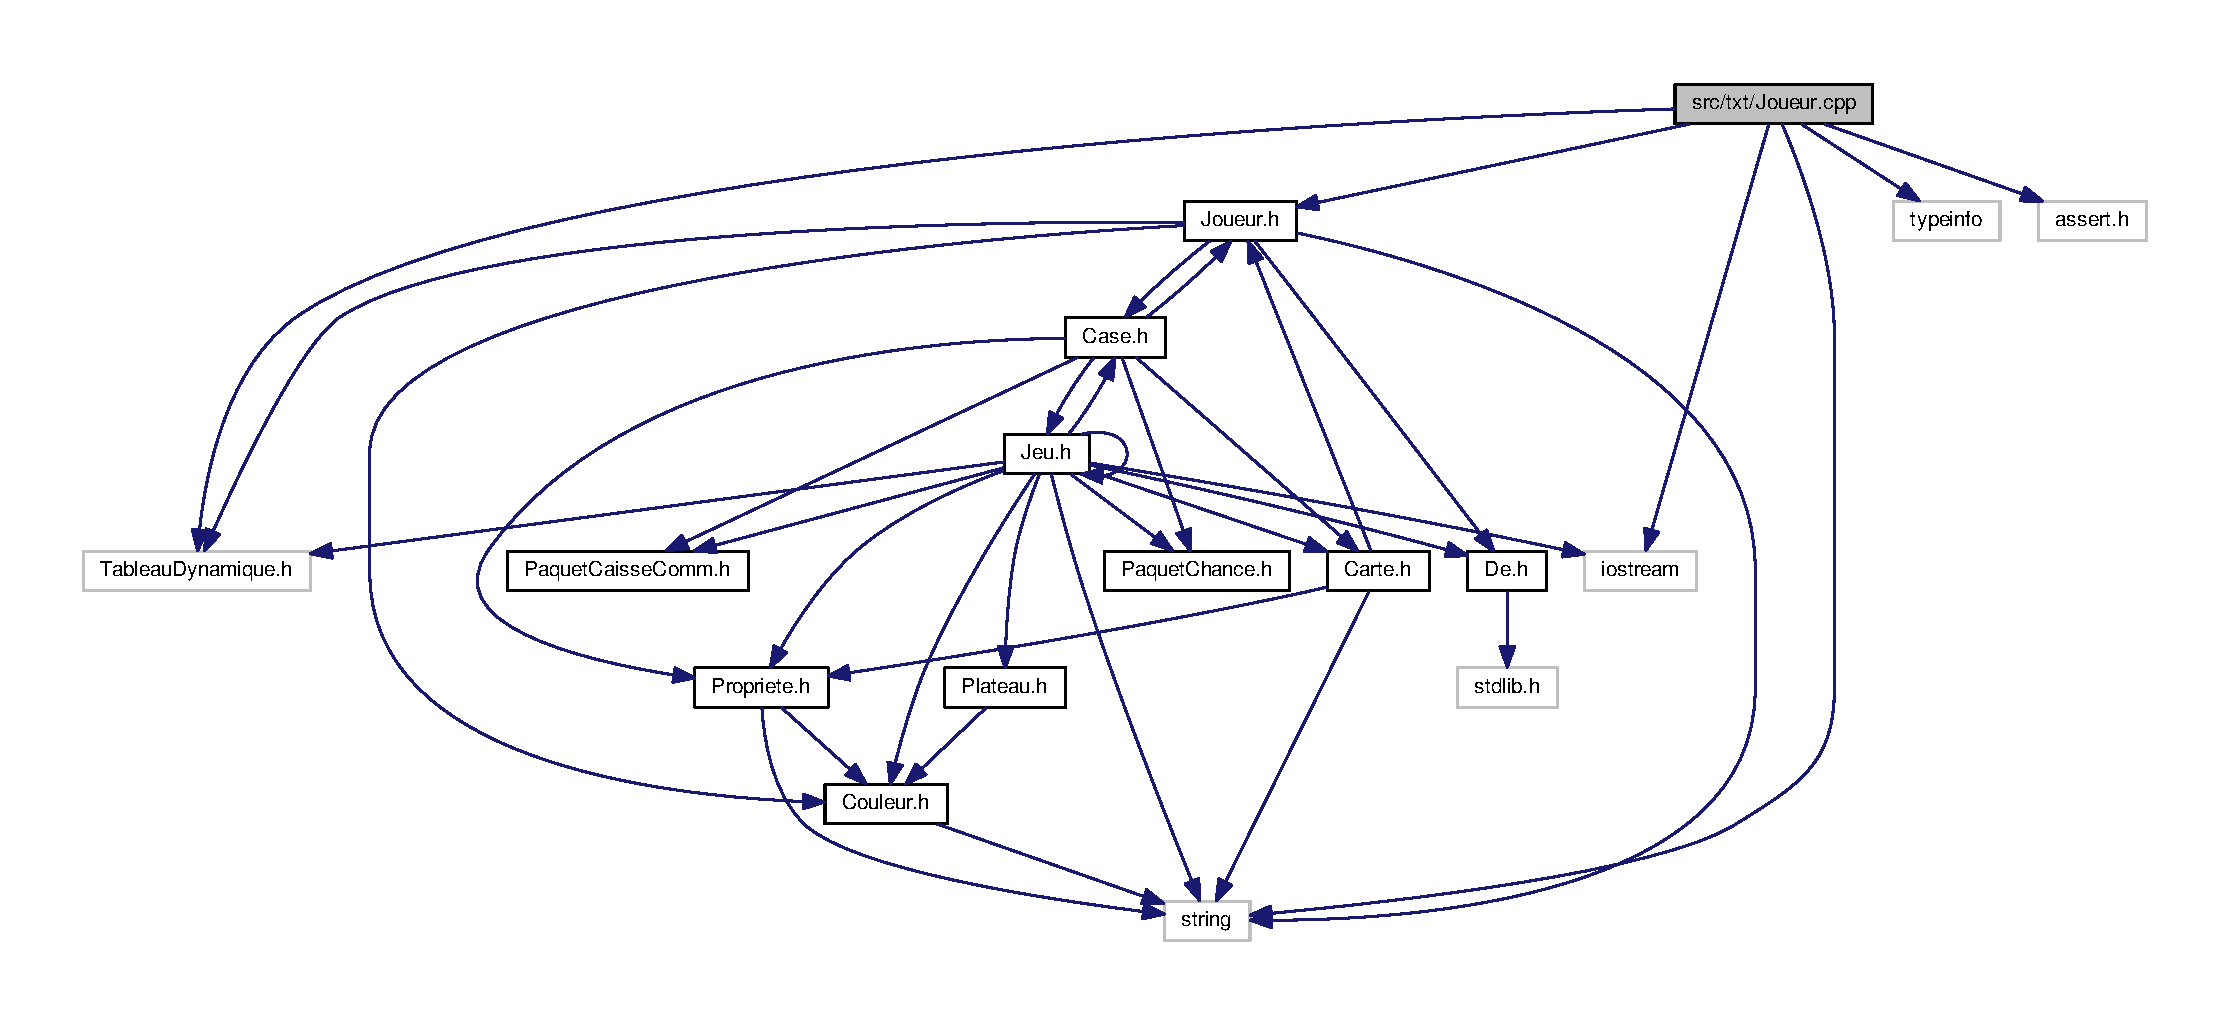
\includegraphics[width=350pt]{Joueur_8cpp__incl}
\end{center}
\end{figure}


\subsection{Description détaillée}
Ce fichier gere les caracteristiques des joueurs ainsi que leurs actions. 

\begin{DoxyAuthor}{Auteur}
Matthieu Cherrier, Kevin Burdin, Tristan Damian
\end{DoxyAuthor}
\begin{DoxyDate}{Date}
2017/04/20 
\end{DoxyDate}

\hypertarget{Joueur_8h}{}\section{Référence du fichier src/txt/\+Joueur.h}
\label{Joueur_8h}\index{src/txt/\+Joueur.\+h@{src/txt/\+Joueur.\+h}}


Ce fichier gere les en-\/tetes des fonctions caracteristiques des joueurs ainsi que leurs actions.  


{\ttfamily \#include $<$string$>$}\\*
{\ttfamily \#include \char`\"{}Case.\+h\char`\"{}}\\*
{\ttfamily \#include \char`\"{}Tableau\+Dynamique.\+h\char`\"{}}\\*
{\ttfamily \#include \char`\"{}Couleur.\+h\char`\"{}}\\*
{\ttfamily \#include \char`\"{}De.\+h\char`\"{}}\\*
Graphe des dépendances par inclusion de Joueur.\+h\+:
\nopagebreak
\begin{figure}[H]
\begin{center}
\leavevmode
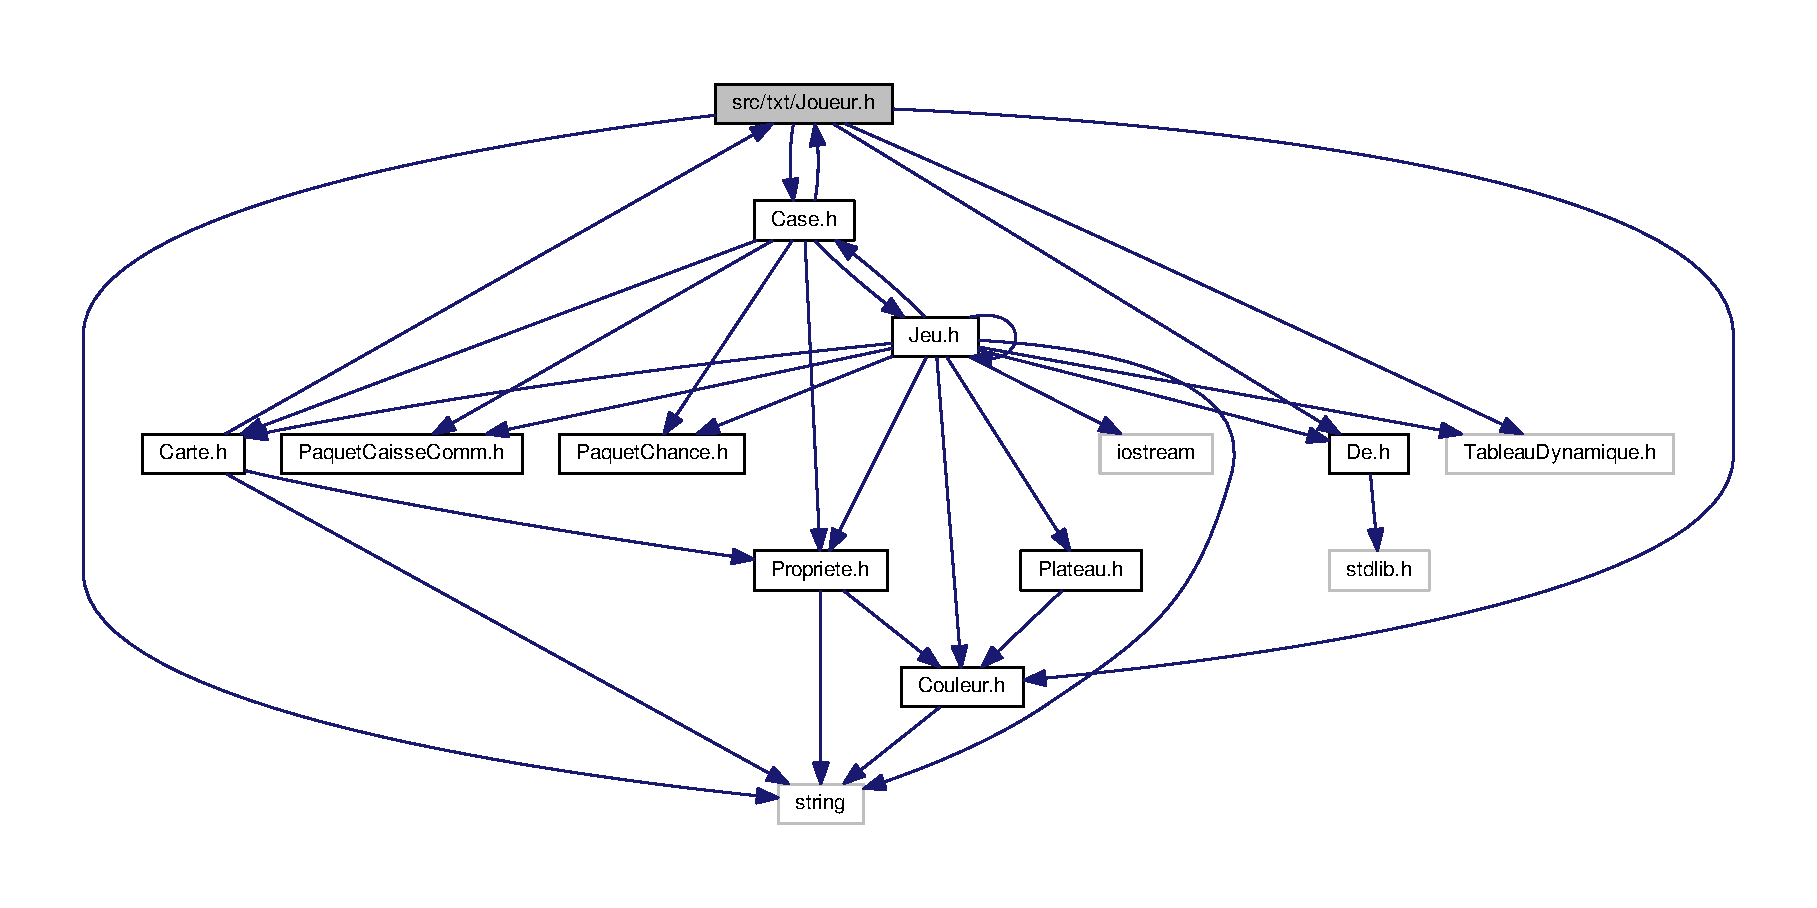
\includegraphics[width=350pt]{Joueur_8h__incl}
\end{center}
\end{figure}
Ce graphe montre quels fichiers incluent directement ou indirectement ce fichier \+:
\nopagebreak
\begin{figure}[H]
\begin{center}
\leavevmode
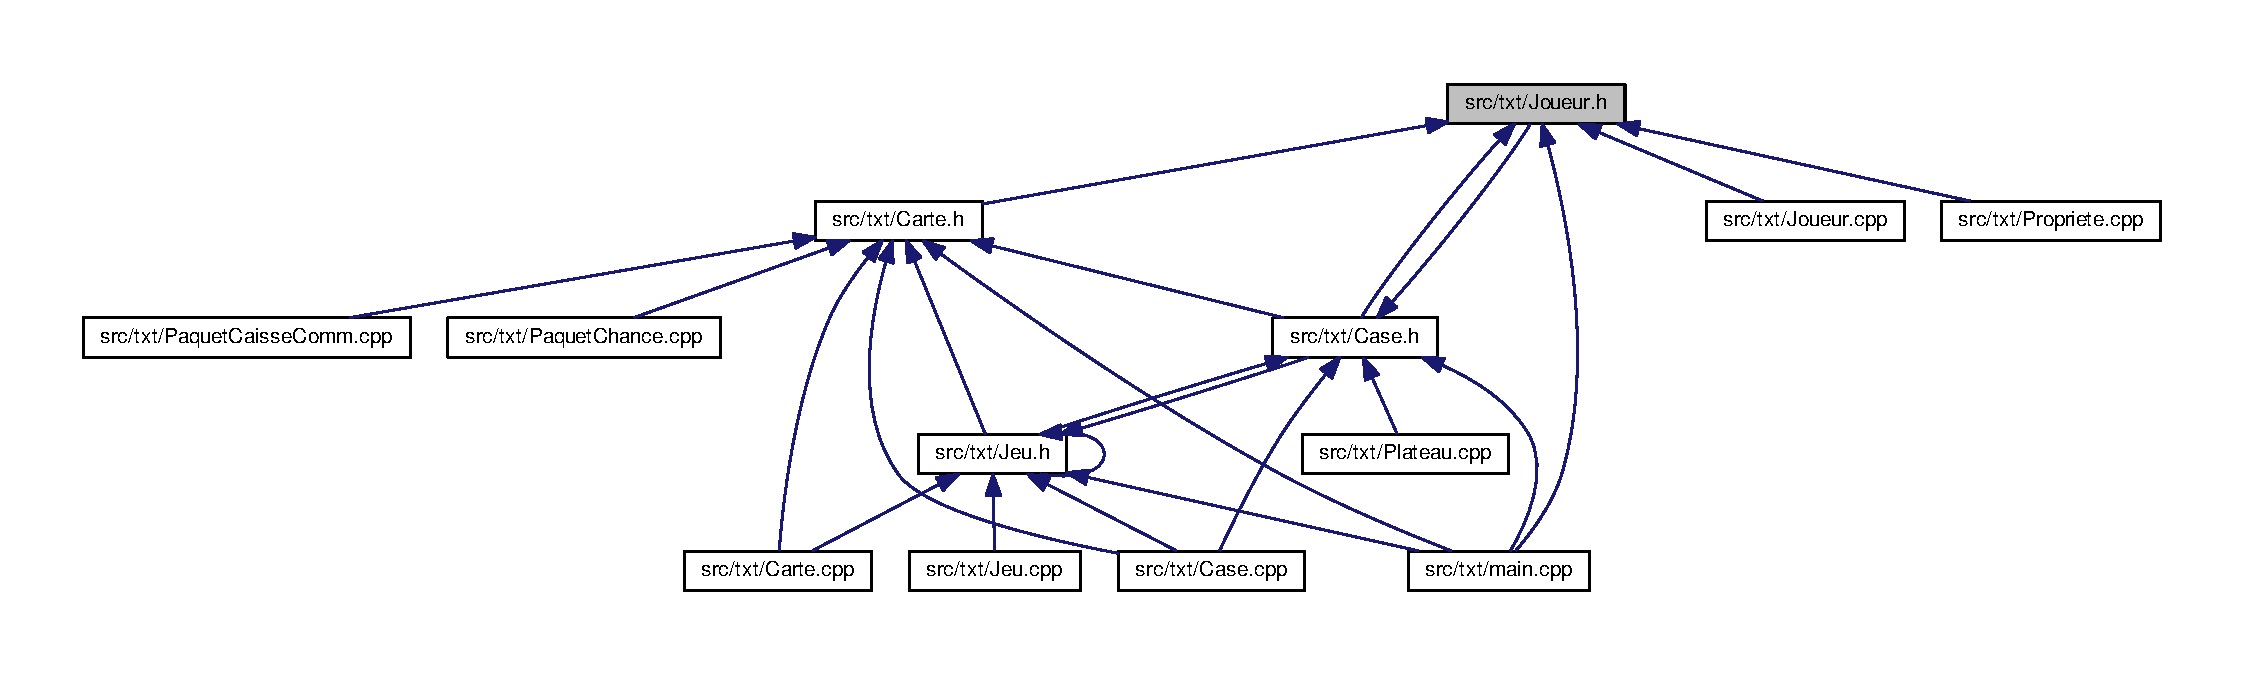
\includegraphics[width=350pt]{Joueur_8h__dep__incl}
\end{center}
\end{figure}
\subsection*{Classes}
\begin{DoxyCompactItemize}
\item 
class \hyperlink{classJoueur}{Joueur}
\end{DoxyCompactItemize}


\subsection{Description détaillée}
Ce fichier gere les en-\/tetes des fonctions caracteristiques des joueurs ainsi que leurs actions. 

\begin{DoxyAuthor}{Auteur}
Matthieu Cherrier, Kevin Burdin, Tristan Damian
\end{DoxyAuthor}
\begin{DoxyDate}{Date}
2017/04/20 
\end{DoxyDate}

\hypertarget{main_8cpp}{}\section{Référence du fichier src/txt/main.cpp}
\label{main_8cpp}\index{src/txt/main.\+cpp@{src/txt/main.\+cpp}}


Ce fichier est le main, le programme principal de T\+HE Monopoly.  


{\ttfamily \#include $<$iostream$>$}\\*
{\ttfamily \#include $<$string$>$}\\*
{\ttfamily \#include \char`\"{}Joueur.\+h\char`\"{}}\\*
{\ttfamily \#include \char`\"{}Couleur.\+h\char`\"{}}\\*
{\ttfamily \#include \char`\"{}Case.\+h\char`\"{}}\\*
{\ttfamily \#include \char`\"{}Plateau.\+h\char`\"{}}\\*
{\ttfamily \#include \char`\"{}Propriete.\+h\char`\"{}}\\*
{\ttfamily \#include \char`\"{}Carte.\+h\char`\"{}}\\*
{\ttfamily \#include \char`\"{}Jeu.\+h\char`\"{}}\\*
{\ttfamily \#include \char`\"{}Paquet\+Chance.\+h\char`\"{}}\\*
{\ttfamily \#include \char`\"{}Paquet\+Caisse\+Comm.\+h\char`\"{}}\\*
{\ttfamily \#include \char`\"{}Tableau\+Dynamique.\+h\char`\"{}}\\*
Graphe des dépendances par inclusion de main.\+cpp\+:
\nopagebreak
\begin{figure}[H]
\begin{center}
\leavevmode
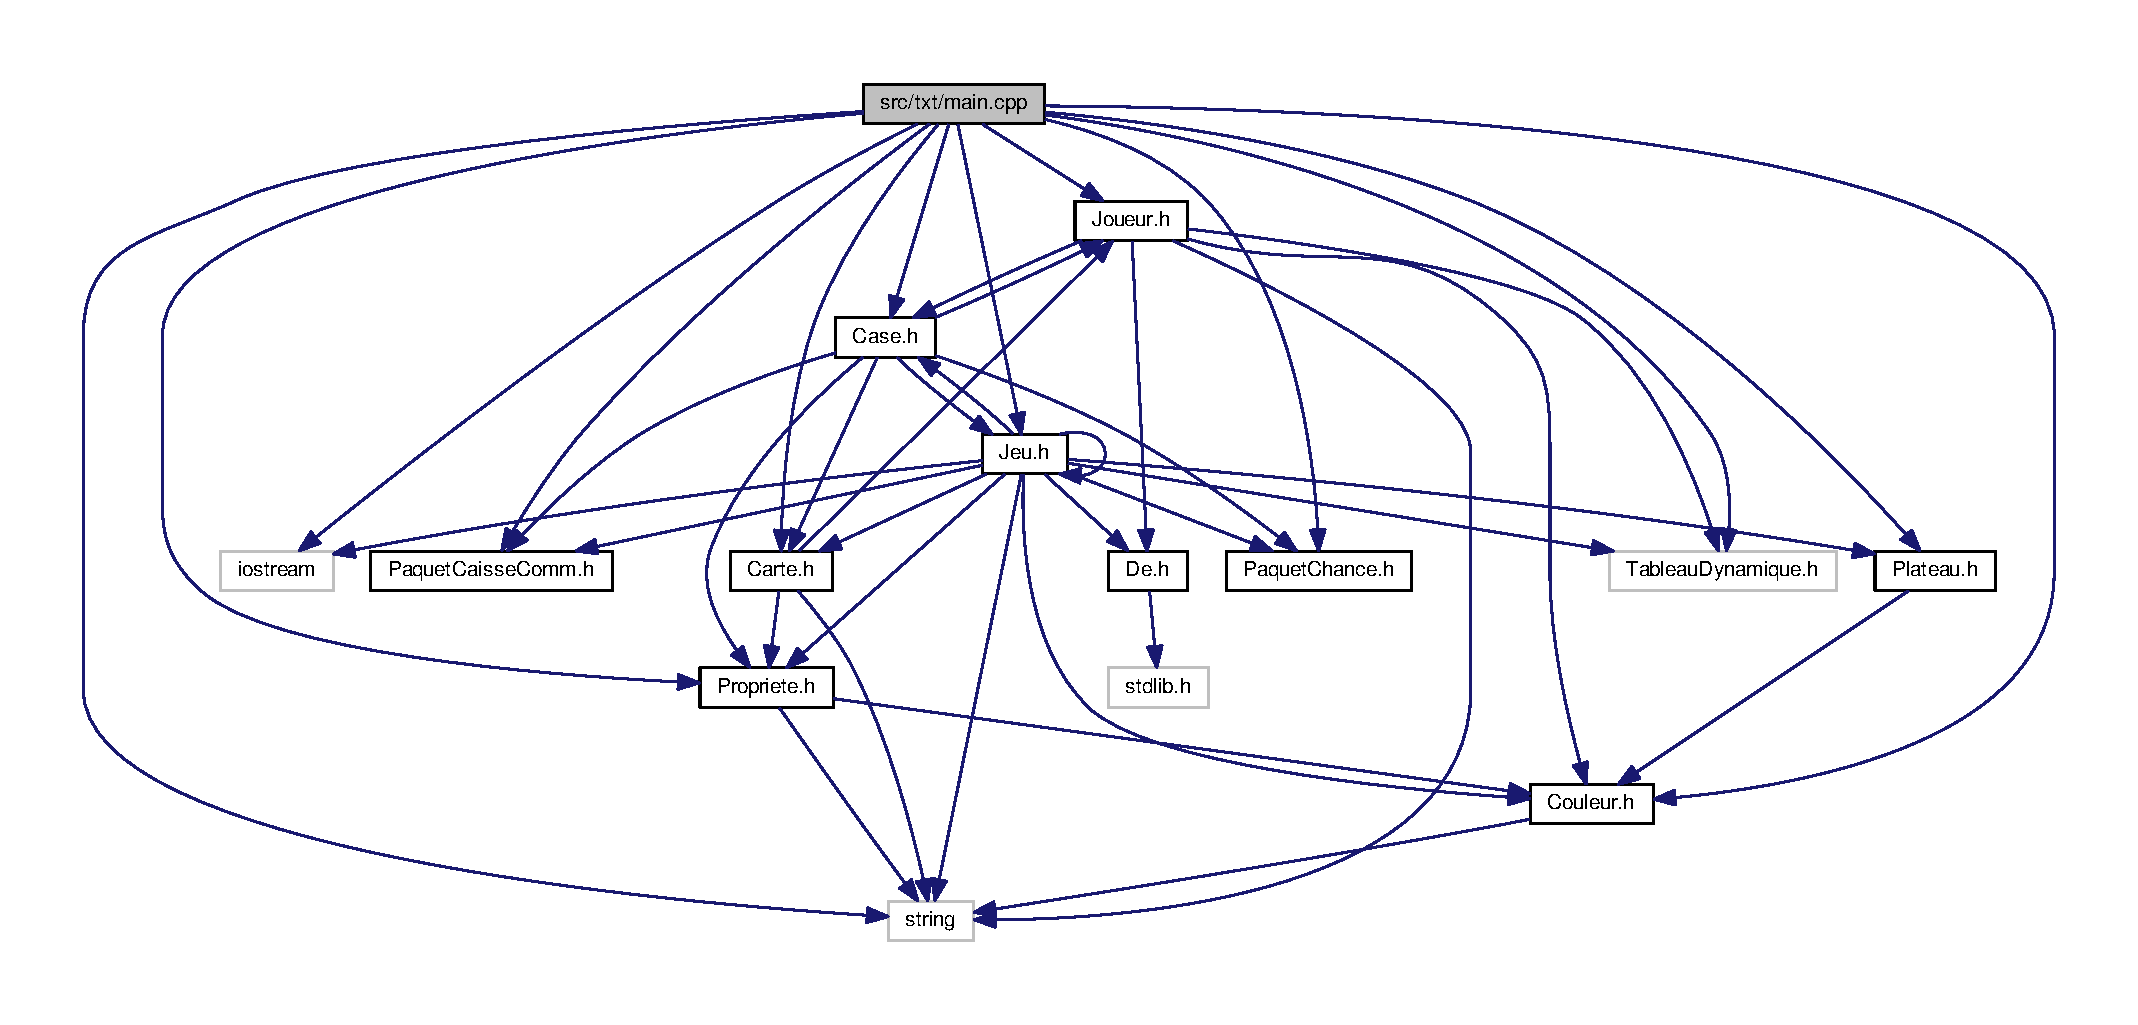
\includegraphics[width=350pt]{main_8cpp__incl}
\end{center}
\end{figure}
\subsection*{Fonctions}
\begin{DoxyCompactItemize}
\item 
int {\bfseries main} (void)\hypertarget{main_8cpp_a840291bc02cba5474a4cb46a9b9566fe}{}\label{main_8cpp_a840291bc02cba5474a4cb46a9b9566fe}

\end{DoxyCompactItemize}


\subsection{Description détaillée}
Ce fichier est le main, le programme principal de T\+HE Monopoly. 

\begin{DoxyAuthor}{Auteur}
Matthieu Cherrier, Kevin Burdin, Tristan Damian
\end{DoxyAuthor}
\begin{DoxyDate}{Date}
2017/04/20 
\end{DoxyDate}

\hypertarget{PaquetCaisseComm_8cpp}{}\section{Référence du fichier src/txt/\+Paquet\+Caisse\+Comm.cpp}
\label{PaquetCaisseComm_8cpp}\index{src/txt/\+Paquet\+Caisse\+Comm.\+cpp@{src/txt/\+Paquet\+Caisse\+Comm.\+cpp}}


Ce fichier contient les fonctions relatives a la gestion des files des cartes caisse de communaute.  


{\ttfamily \#include \char`\"{}Carte.\+h\char`\"{}}\\*
{\ttfamily \#include \char`\"{}Paquet\+Caisse\+Comm.\+h\char`\"{}}\\*
{\ttfamily \#include $<$iostream$>$}\\*
{\ttfamily \#include $<$stdlib.\+h$>$}\\*
{\ttfamily \#include $<$string$>$}\\*
Graphe des dépendances par inclusion de Paquet\+Caisse\+Comm.\+cpp\+:
\nopagebreak
\begin{figure}[H]
\begin{center}
\leavevmode
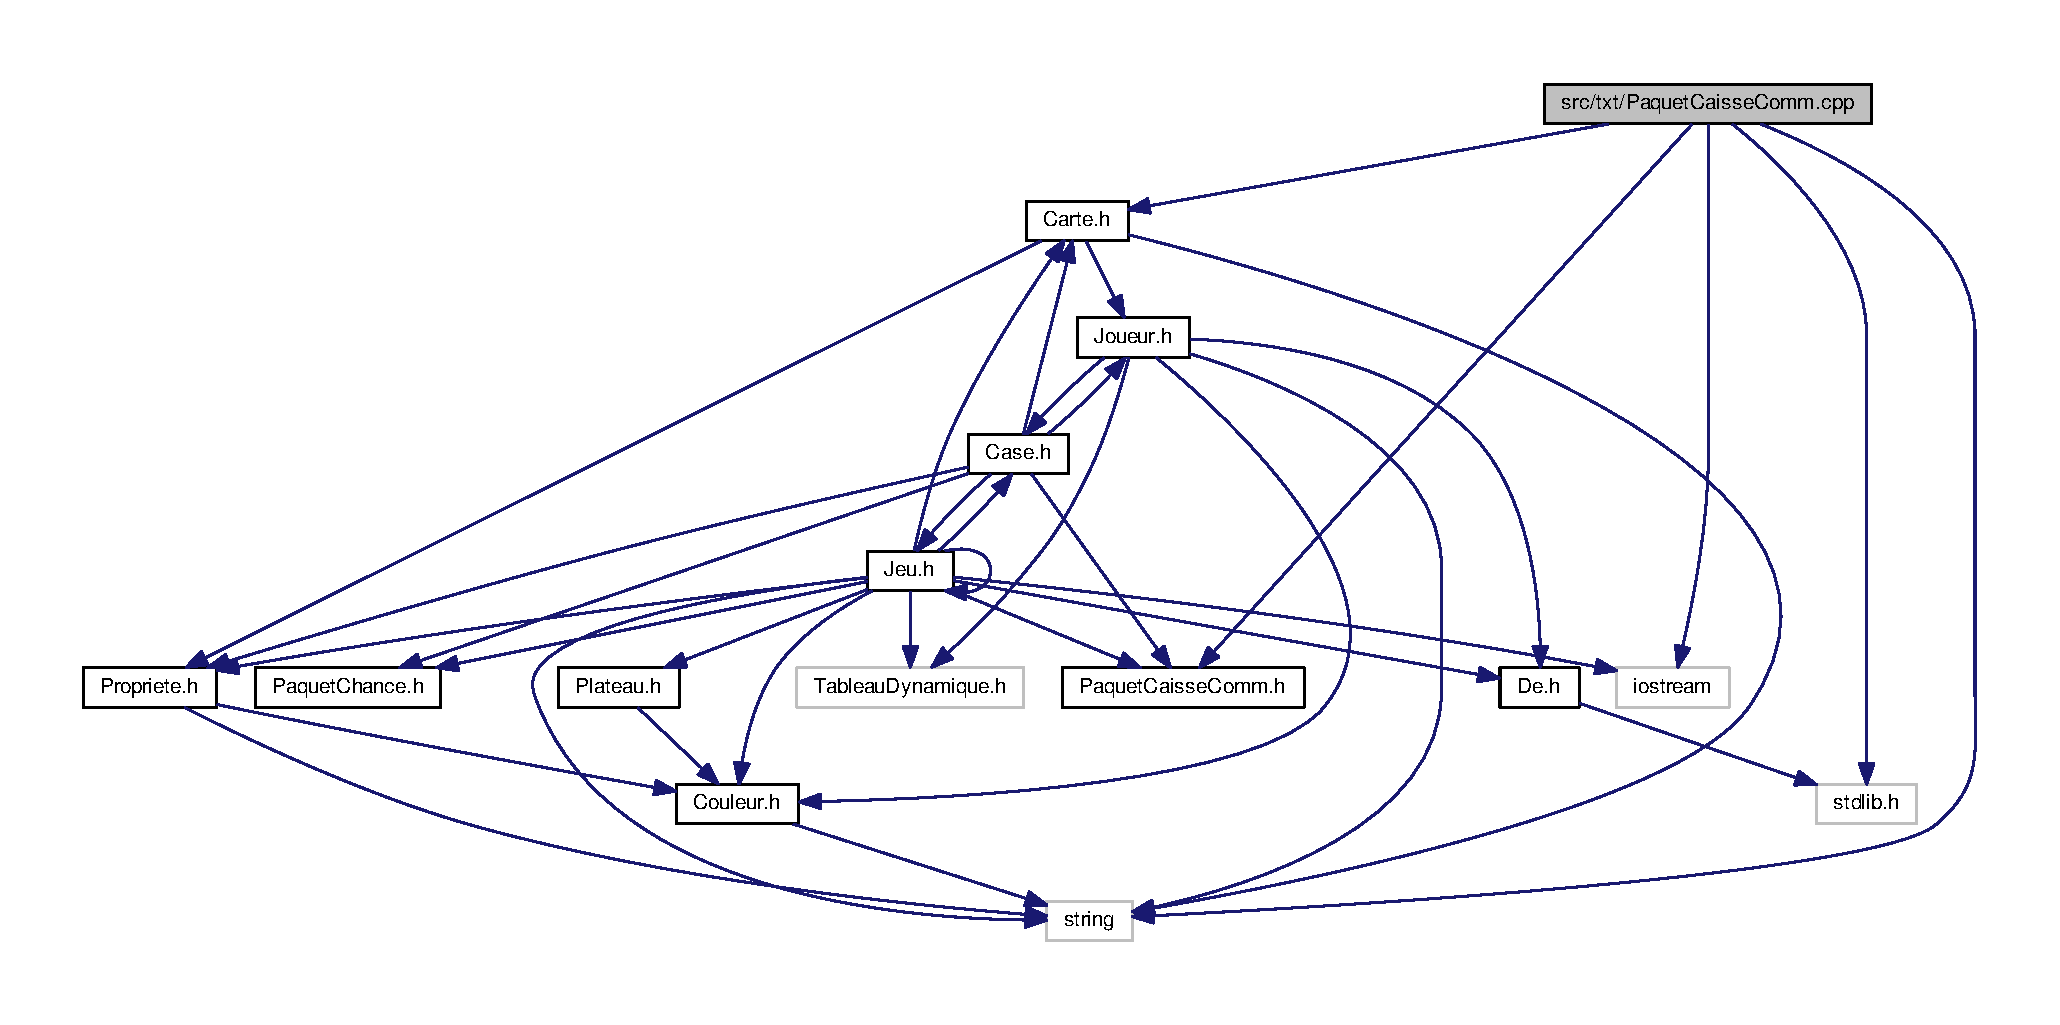
\includegraphics[width=350pt]{PaquetCaisseComm_8cpp__incl}
\end{center}
\end{figure}


\subsection{Description détaillée}
Ce fichier contient les fonctions relatives a la gestion des files des cartes caisse de communaute. 

\begin{DoxyAuthor}{Auteur}
Matthieu Cherrier, Kevin Burdin, Tristan Damian
\end{DoxyAuthor}
\begin{DoxyDate}{Date}
2017/04/20 
\end{DoxyDate}

\hypertarget{PaquetCaisseComm_8h}{}\section{Référence du fichier src/txt/\+Paquet\+Caisse\+Comm.h}
\label{PaquetCaisseComm_8h}\index{src/txt/\+Paquet\+Caisse\+Comm.\+h@{src/txt/\+Paquet\+Caisse\+Comm.\+h}}


Ce fichier contient les en-\/tetes des fonctions relatives a la gestion des files des cartes caisse de communaute.  


Ce graphe montre quels fichiers incluent directement ou indirectement ce fichier \+:
\nopagebreak
\begin{figure}[H]
\begin{center}
\leavevmode
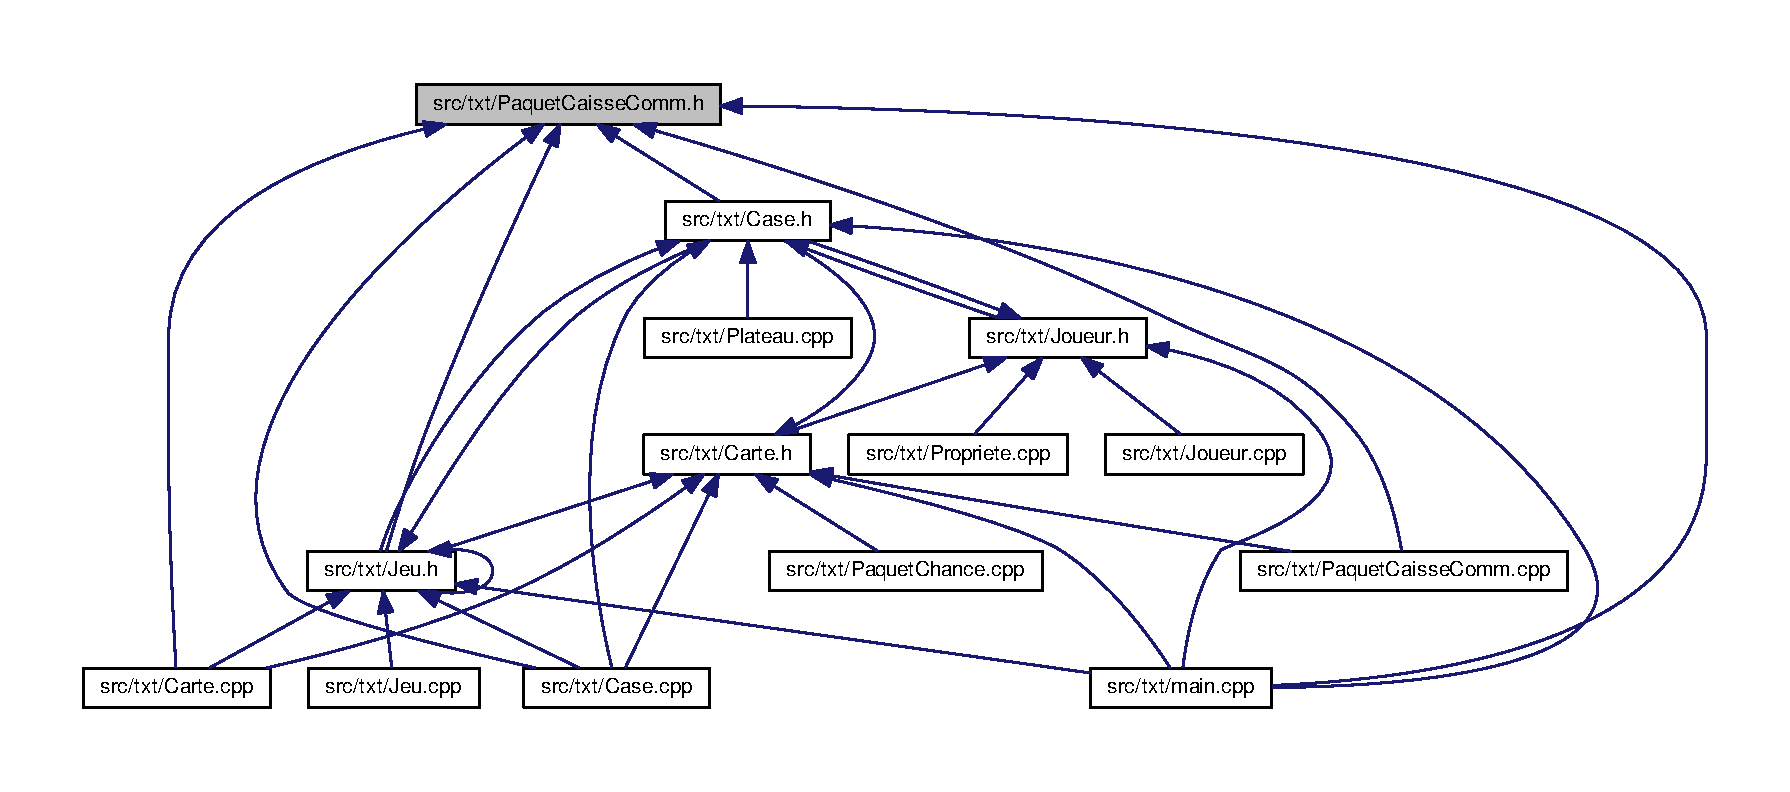
\includegraphics[width=350pt]{PaquetCaisseComm_8h__dep__incl}
\end{center}
\end{figure}
\subsection*{Classes}
\begin{DoxyCompactItemize}
\item 
class \hyperlink{classPaquetCaisseComm}{Paquet\+Caisse\+Comm}
\item 
struct \hyperlink{structPaquetCaisseComm_1_1Cellule}{Paquet\+Caisse\+Comm\+::\+Cellule}
\end{DoxyCompactItemize}


\subsection{Description détaillée}
Ce fichier contient les en-\/tetes des fonctions relatives a la gestion des files des cartes caisse de communaute. 

\begin{DoxyAuthor}{Auteur}
Matthieu Cherrier, Kevin Burdin, Tristan Damian
\end{DoxyAuthor}
\begin{DoxyDate}{Date}
2017/04/20 
\end{DoxyDate}

\hypertarget{PaquetChance_8cpp}{}\section{Référence du fichier src/txt/\+Paquet\+Chance.cpp}
\label{PaquetChance_8cpp}\index{src/txt/\+Paquet\+Chance.\+cpp@{src/txt/\+Paquet\+Chance.\+cpp}}


Ce fichier contient les fonctions relatives a la gestion des files des cartes chance.  


{\ttfamily \#include \char`\"{}Paquet\+Chance.\+h\char`\"{}}\\*
{\ttfamily \#include $<$string$>$}\\*
{\ttfamily \#include \char`\"{}Carte.\+h\char`\"{}}\\*
{\ttfamily \#include $<$iostream$>$}\\*
{\ttfamily \#include $<$stdlib.\+h$>$}\\*
Graphe des dépendances par inclusion de Paquet\+Chance.\+cpp\+:
\nopagebreak
\begin{figure}[H]
\begin{center}
\leavevmode
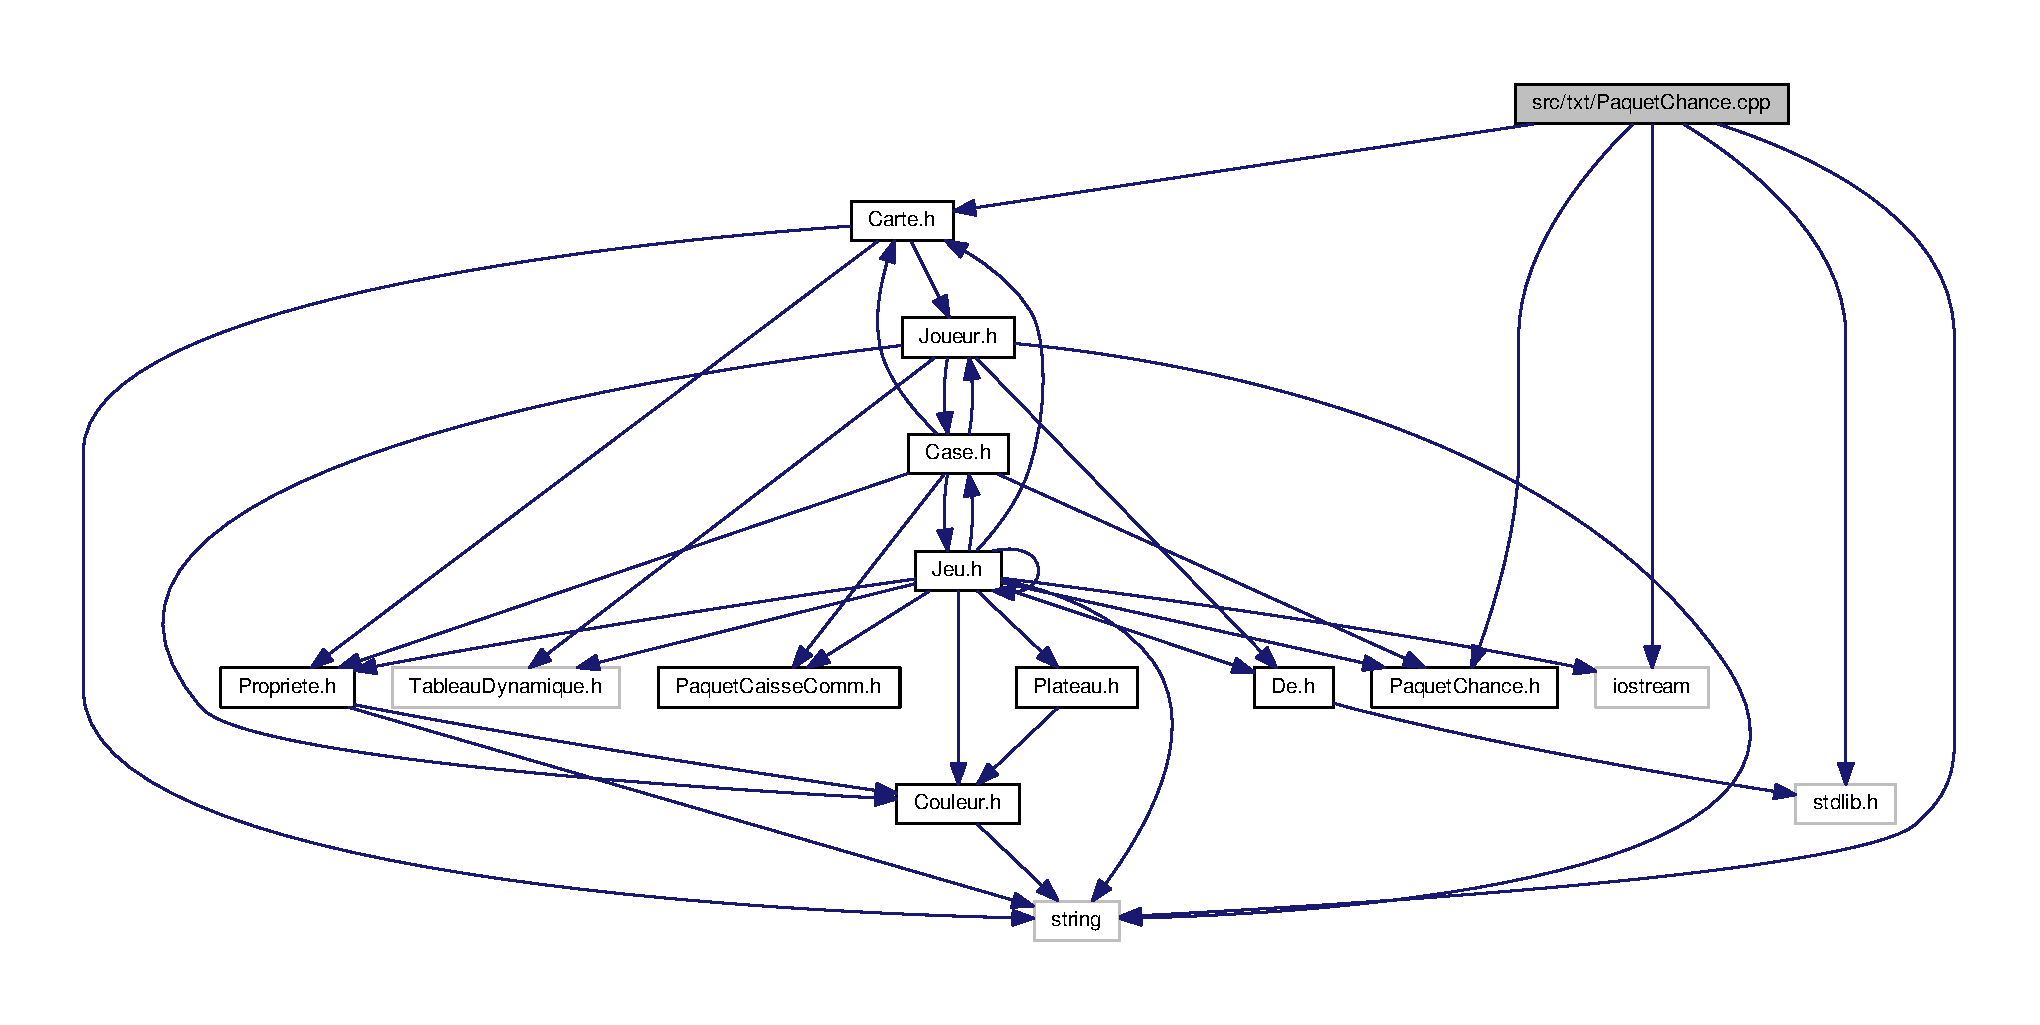
\includegraphics[width=350pt]{PaquetChance_8cpp__incl}
\end{center}
\end{figure}


\subsection{Description détaillée}
Ce fichier contient les fonctions relatives a la gestion des files des cartes chance. 

\begin{DoxyAuthor}{Auteur}
Matthieu Cherrier, Kevin Burdin, Tristan Damian
\end{DoxyAuthor}
\begin{DoxyDate}{Date}
2017/04/20 
\end{DoxyDate}

\hypertarget{PaquetChance_8h}{}\section{Référence du fichier src/txt/\+Paquet\+Chance.h}
\label{PaquetChance_8h}\index{src/txt/\+Paquet\+Chance.\+h@{src/txt/\+Paquet\+Chance.\+h}}


Ce fichier contient les en-\/tetes des fonctions relatives a la gestion des files des cartes chance.  


Ce graphe montre quels fichiers incluent directement ou indirectement ce fichier \+:
\nopagebreak
\begin{figure}[H]
\begin{center}
\leavevmode
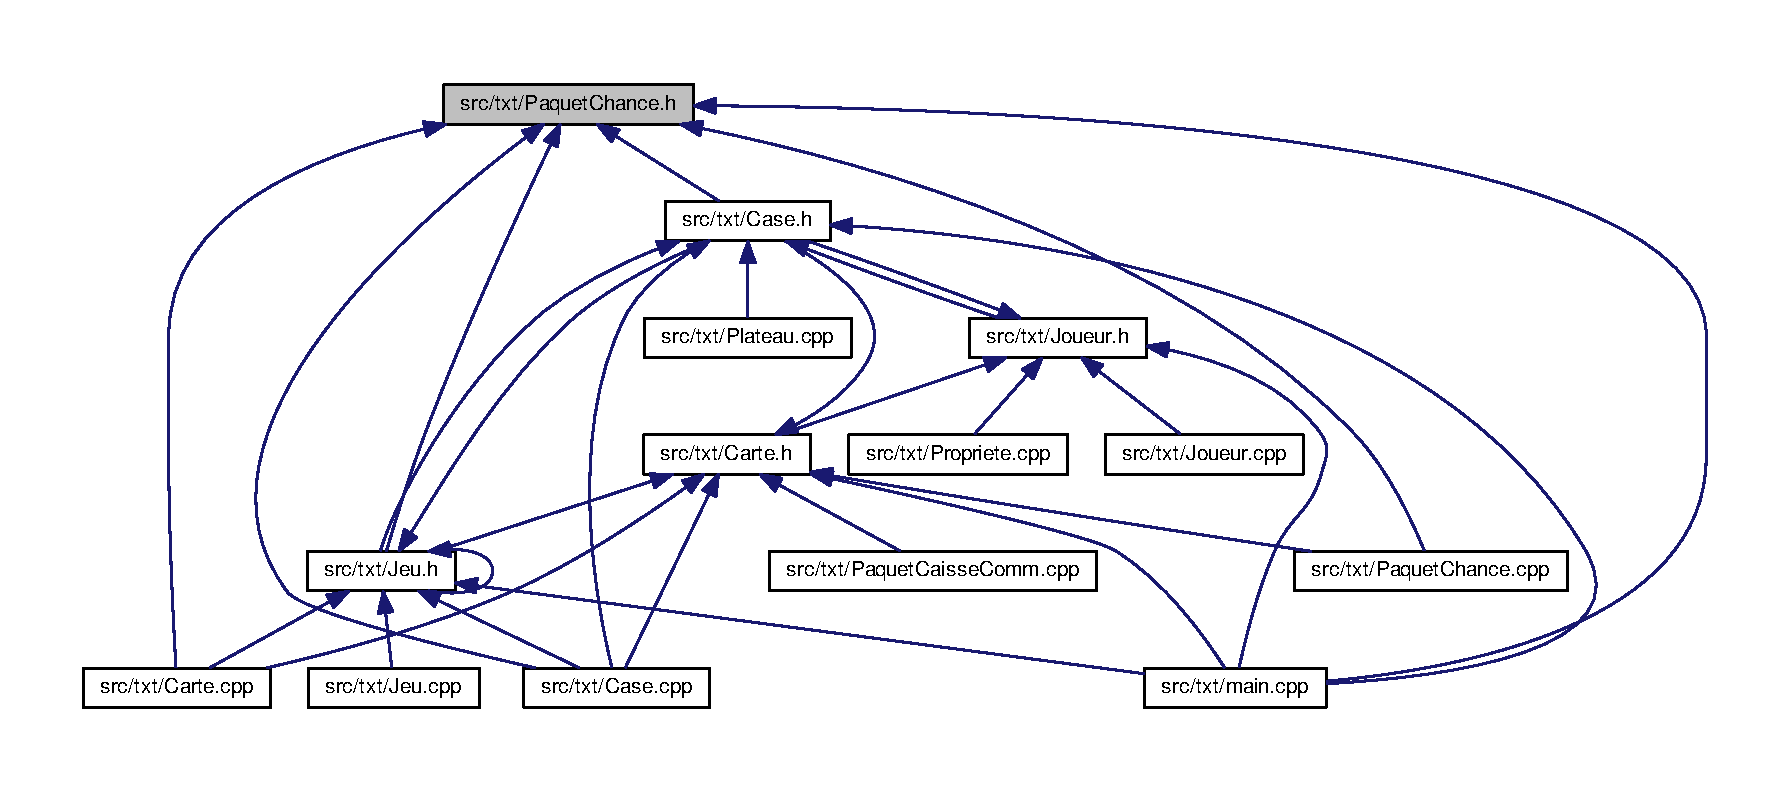
\includegraphics[width=350pt]{PaquetChance_8h__dep__incl}
\end{center}
\end{figure}
\subsection*{Classes}
\begin{DoxyCompactItemize}
\item 
class \hyperlink{classPaquetChance}{Paquet\+Chance}
\item 
struct \hyperlink{structPaquetChance_1_1Cellule}{Paquet\+Chance\+::\+Cellule}
\end{DoxyCompactItemize}


\subsection{Description détaillée}
Ce fichier contient les en-\/tetes des fonctions relatives a la gestion des files des cartes chance. 

\begin{DoxyAuthor}{Auteur}
Matthieu Cherrier, Kevin Burdin, Tristan Damian
\end{DoxyAuthor}
\begin{DoxyDate}{Date}
2017/04/20 
\end{DoxyDate}

\hypertarget{Plateau_8cpp}{}\section{Référence du fichier src/txt/\+Plateau.cpp}
\label{Plateau_8cpp}\index{src/txt/\+Plateau.\+cpp@{src/txt/\+Plateau.\+cpp}}


Ce fichier contient les fonctions relatives a la gestion du plateau.  


{\ttfamily \#include \char`\"{}Plateau.\+h\char`\"{}}\\*
{\ttfamily \#include \char`\"{}Case.\+h\char`\"{}}\\*
{\ttfamily \#include $<$string$>$}\\*
Graphe des dépendances par inclusion de Plateau.\+cpp\+:
\nopagebreak
\begin{figure}[H]
\begin{center}
\leavevmode
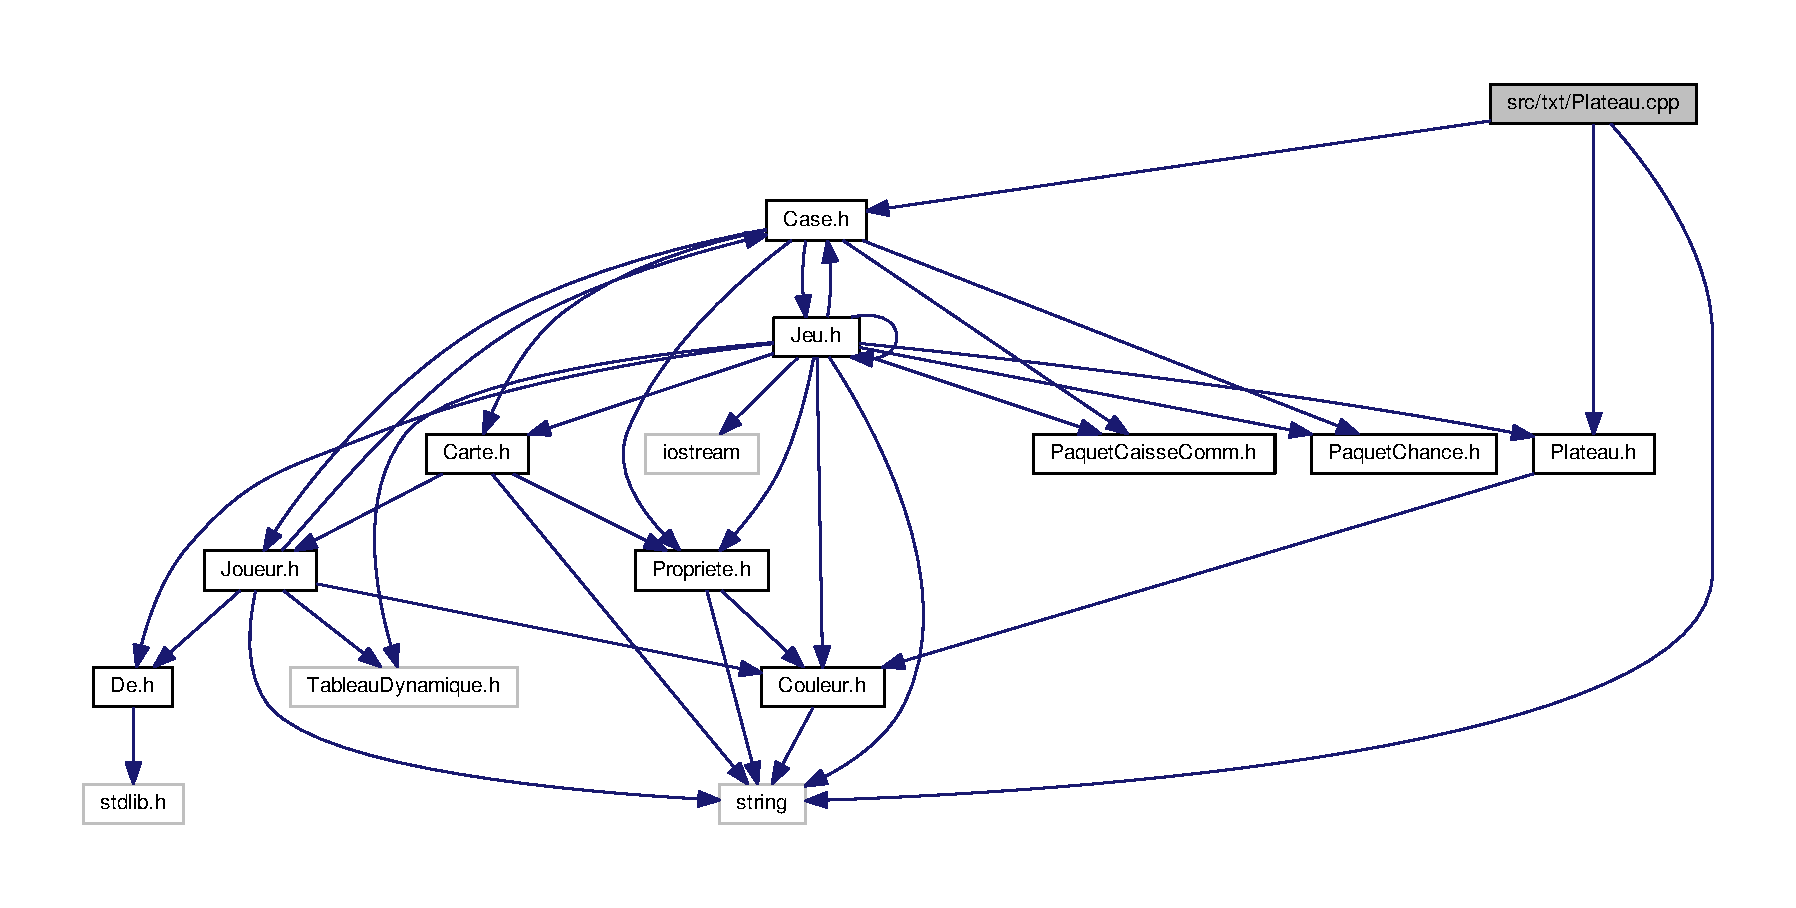
\includegraphics[width=350pt]{Plateau_8cpp__incl}
\end{center}
\end{figure}


\subsection{Description détaillée}
Ce fichier contient les fonctions relatives a la gestion du plateau. 

\begin{DoxyAuthor}{Auteur}
Matthieu Cherrier, Kevin Burdin, Tristan Damian
\end{DoxyAuthor}
\begin{DoxyDate}{Date}
2017/04/20 
\end{DoxyDate}

\hypertarget{Plateau_8h}{}\section{Référence du fichier src/txt/\+Plateau.h}
\label{Plateau_8h}\index{src/txt/\+Plateau.\+h@{src/txt/\+Plateau.\+h}}


Ce fichier contient les en-\/tetes des fonctions relatives a la gestion du plateau.  


{\ttfamily \#include \char`\"{}Couleur.\+h\char`\"{}}\\*
Graphe des dépendances par inclusion de Plateau.\+h\+:
\nopagebreak
\begin{figure}[H]
\begin{center}
\leavevmode
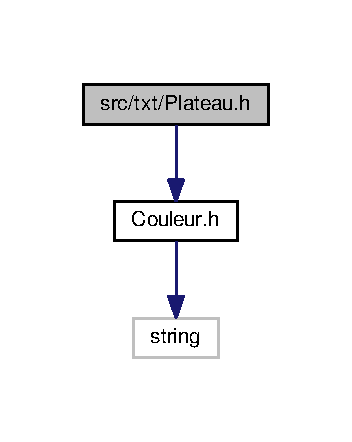
\includegraphics[width=169pt]{Plateau_8h__incl}
\end{center}
\end{figure}
Ce graphe montre quels fichiers incluent directement ou indirectement ce fichier \+:
\nopagebreak
\begin{figure}[H]
\begin{center}
\leavevmode
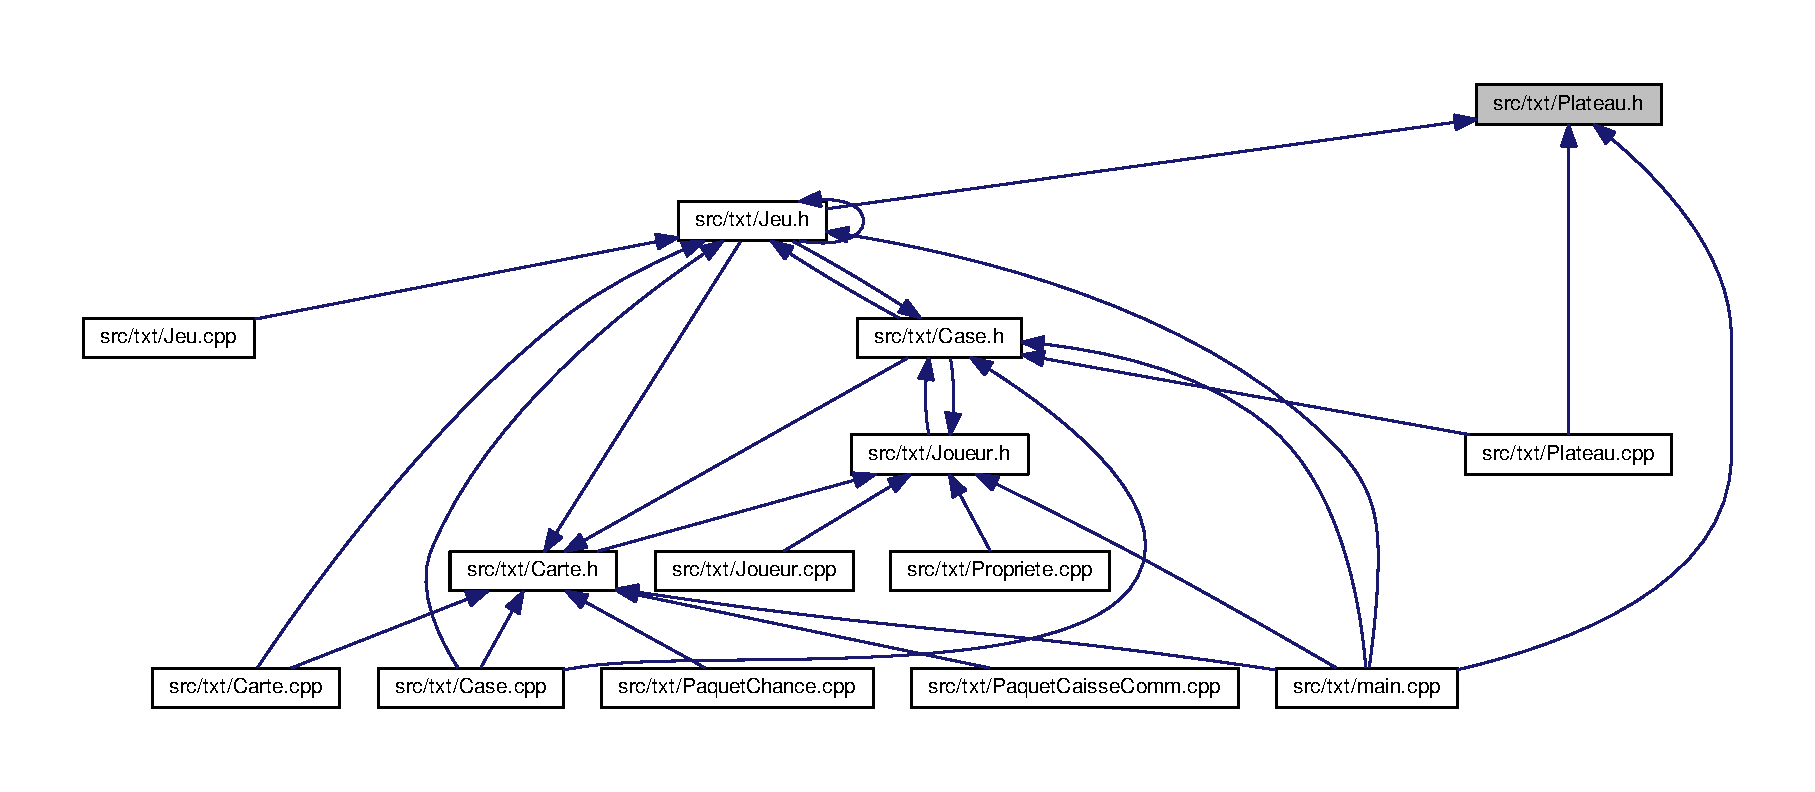
\includegraphics[width=350pt]{Plateau_8h__dep__incl}
\end{center}
\end{figure}
\subsection*{Classes}
\begin{DoxyCompactItemize}
\item 
class \hyperlink{classPlateau}{Plateau}
\end{DoxyCompactItemize}


\subsection{Description détaillée}
Ce fichier contient les en-\/tetes des fonctions relatives a la gestion du plateau. 

\begin{DoxyAuthor}{Auteur}
Matthieu Cherrier, Kevin Burdin, Tristan Damian
\end{DoxyAuthor}
\begin{DoxyDate}{Date}
2017/04/20 
\end{DoxyDate}

\hypertarget{Propriete_8cpp}{}\section{Référence du fichier src/txt/\+Propriete.cpp}
\label{Propriete_8cpp}\index{src/txt/\+Propriete.\+cpp@{src/txt/\+Propriete.\+cpp}}


Ce fichier contient les fonctions relatives a la gestion des proprietes (cases) du plateau.  


{\ttfamily \#include \char`\"{}Propriete.\+h\char`\"{}}\\*
{\ttfamily \#include \char`\"{}Joueur.\+h\char`\"{}}\\*
{\ttfamily \#include \char`\"{}Couleur.\+h\char`\"{}}\\*
{\ttfamily \#include $<$string$>$}\\*
{\ttfamily \#include $<$iostream$>$}\\*
Graphe des dépendances par inclusion de Propriete.\+cpp\+:
\nopagebreak
\begin{figure}[H]
\begin{center}
\leavevmode
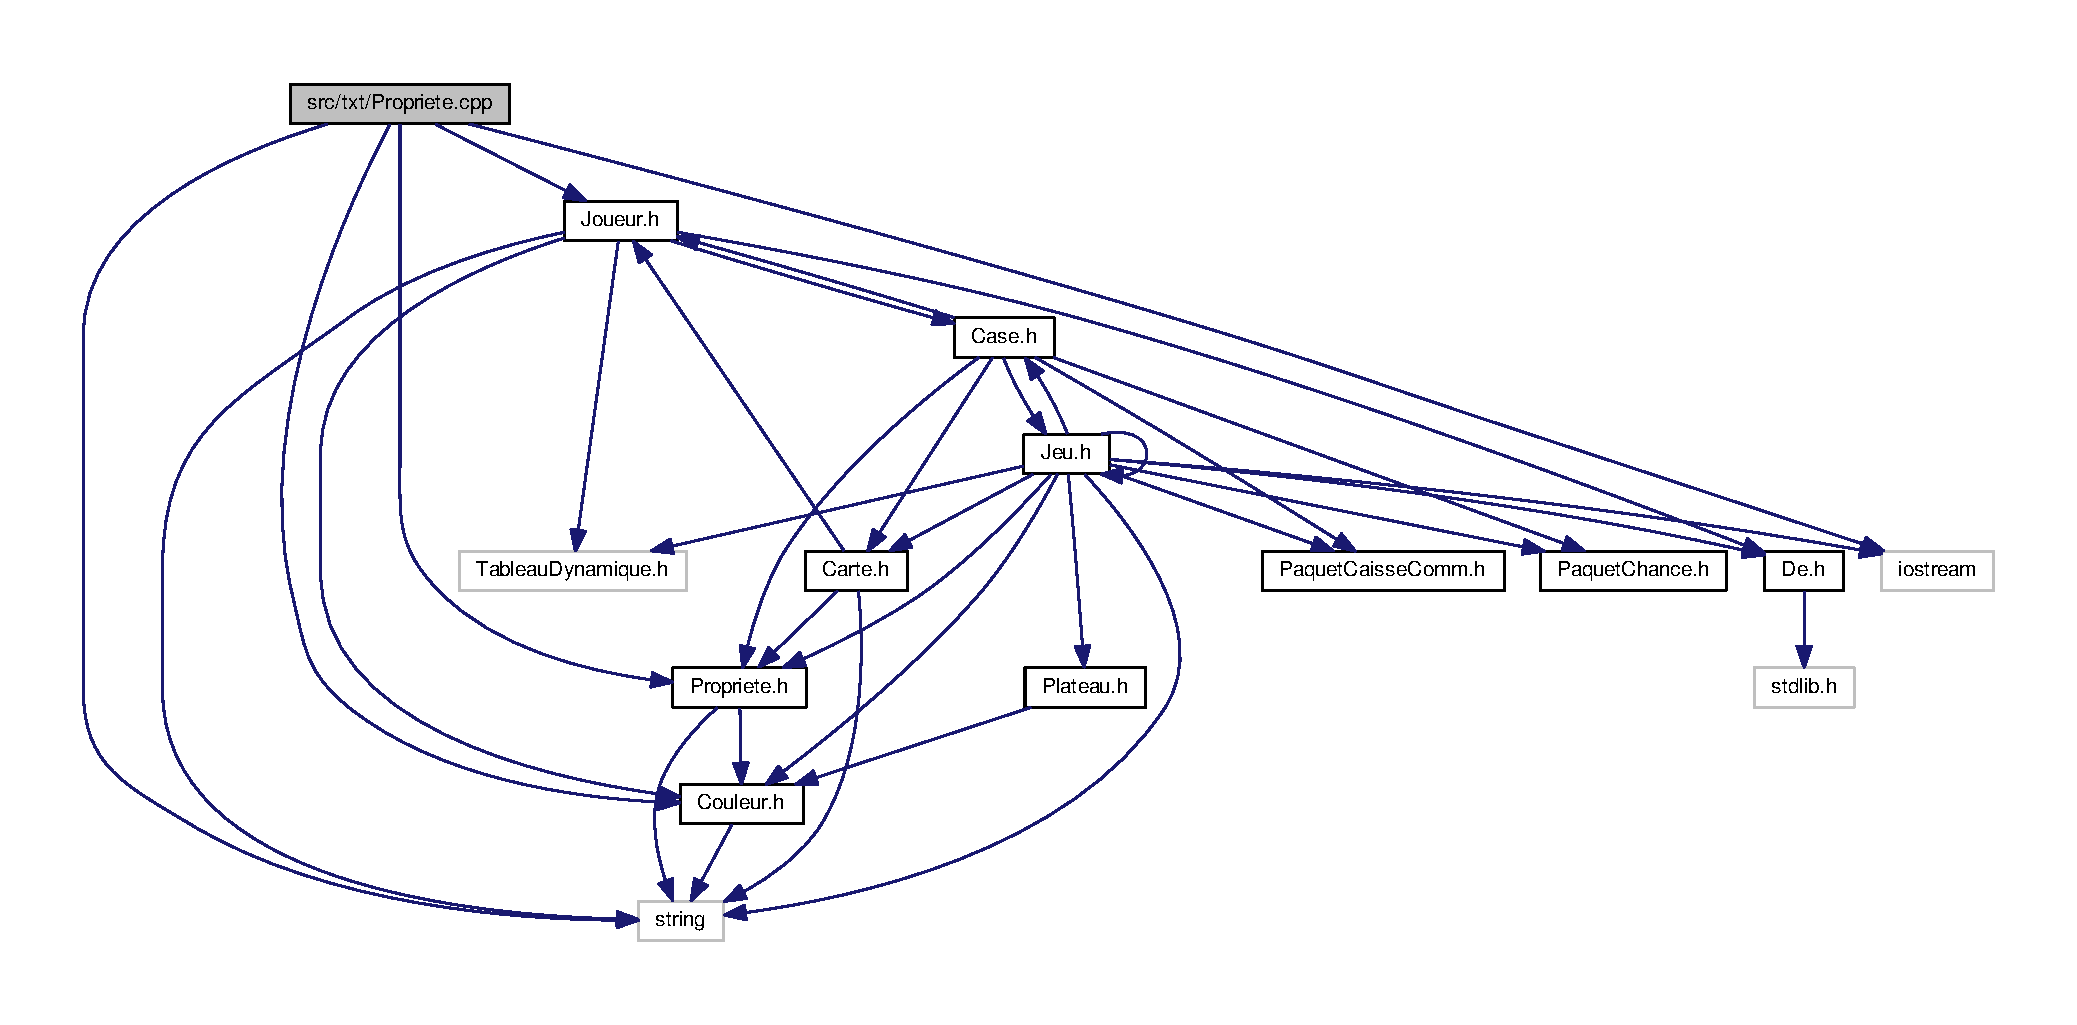
\includegraphics[width=350pt]{Propriete_8cpp__incl}
\end{center}
\end{figure}


\subsection{Description détaillée}
Ce fichier contient les fonctions relatives a la gestion des proprietes (cases) du plateau. 

\begin{DoxyAuthor}{Auteur}
Matthieu Cherrier, Kevin Burdin, Tristan Damian
\end{DoxyAuthor}
\begin{DoxyDate}{Date}
2017/04/20 
\end{DoxyDate}

\hypertarget{Propriete_8h}{}\section{Référence du fichier src/txt/\+Propriete.h}
\label{Propriete_8h}\index{src/txt/\+Propriete.\+h@{src/txt/\+Propriete.\+h}}


Ce fichier contient les en-\/tetes des fonctions relatives a la gestion des proprietes (cases) du plateau.  


{\ttfamily \#include $<$string$>$}\\*
{\ttfamily \#include \char`\"{}Couleur.\+h\char`\"{}}\\*
Graphe des dépendances par inclusion de Propriete.\+h\+:
\nopagebreak
\begin{figure}[H]
\begin{center}
\leavevmode
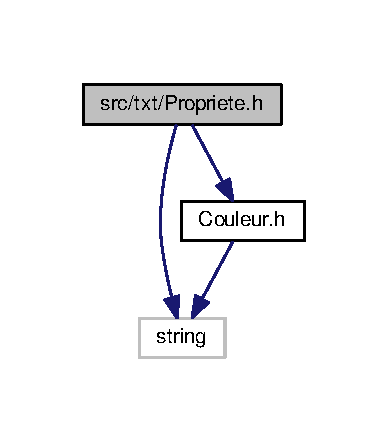
\includegraphics[width=186pt]{Propriete_8h__incl}
\end{center}
\end{figure}
Ce graphe montre quels fichiers incluent directement ou indirectement ce fichier \+:
\nopagebreak
\begin{figure}[H]
\begin{center}
\leavevmode
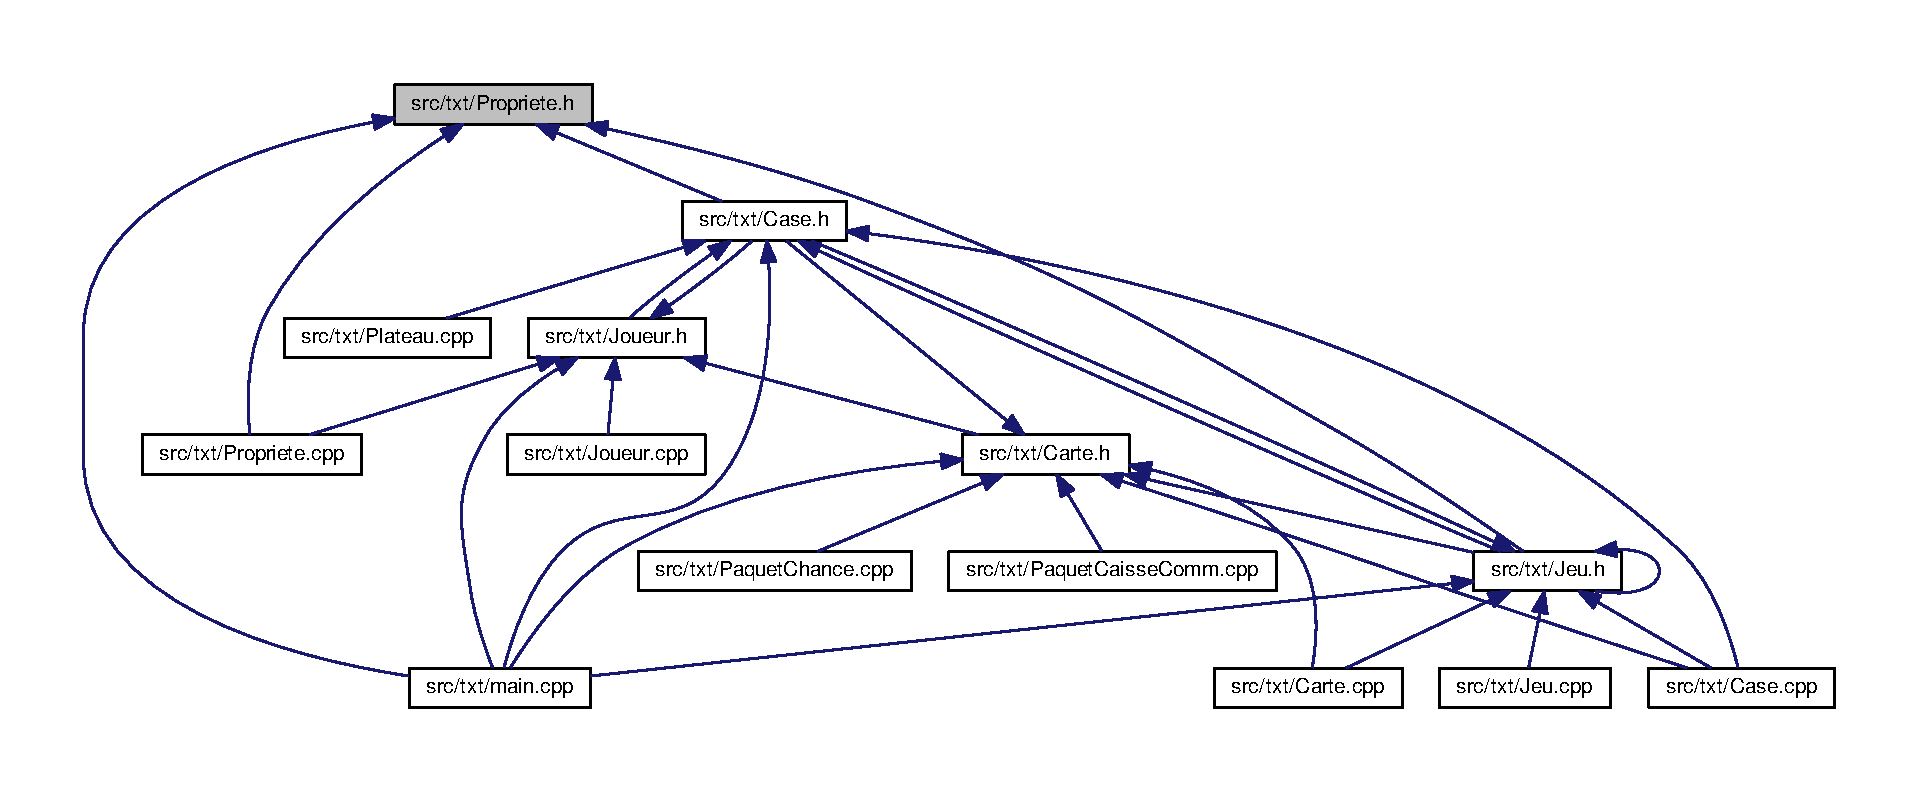
\includegraphics[width=350pt]{Propriete_8h__dep__incl}
\end{center}
\end{figure}
\subsection*{Classes}
\begin{DoxyCompactItemize}
\item 
class \hyperlink{classPropriete}{Propriete}
\end{DoxyCompactItemize}


\subsection{Description détaillée}
Ce fichier contient les en-\/tetes des fonctions relatives a la gestion des proprietes (cases) du plateau. 

\begin{DoxyAuthor}{Auteur}
Matthieu Cherrier, Kevin Burdin, Tristan Damian
\end{DoxyAuthor}
\begin{DoxyDate}{Date}
2017/04/20 
\end{DoxyDate}

%--- End generated contents ---

% Index
\backmatter
\newpage
\phantomsection
\clearemptydoublepage
\addcontentsline{toc}{chapter}{Index}
\printindex

\end{document}
